%%%%%%%%%%%%%%%%%%%%%%%%%%%%%%%%%%%%%%%%%%%%%%%%%%%%%%%%%%%%%%%%%%%%%%
% Template for a UBC-compliant dissertation
% At the minimum, you will need to change the information found
% after the "Document meta-data"
%
%!TEX TS-program = pdflatex
%!TEX encoding = UTF-8 Unicode

%% The ubcdiss class provides several options:
%%   gpscopy (aka fogscopy)
%%       set parameters to exactly how GPS specifies
%%         * single-sided
%%         * page-numbering starts from title page
%%         * the lists of figures and tables have each entry prefixed
%%           with 'Figure' or 'Table'
%%       This can be tested by `\ifgpscopy ... \else ... \fi'
%%   10pt, 11pt, 12pt
%%       set default font size
%%   oneside, twoside
%%       whether to format for single-sided or double-sided printing
%%   balanced
%%       when double-sided, ensure page content is centred
%%       rather than slightly offset (the default)
%%   singlespacing, onehalfspacing, doublespacing
%%       set default inter-line text spacing; the ubcdiss class
%%       provides \textspacing to revert to this configured spacing
%%   draft
%%       disable more intensive processing, such as including
%%       graphics, etc.
%%

% For submission to GPS
\documentclass[gpscopy,doublespacing,11pt]{ubcdiss}

% For your own copies (looks nicer)
% \documentclass[balanced,twoside,11pt]{ubcdiss}



%%%%%%%%%%%%%%%%%%%%%%%%%%%%%%%%%%%%%%%%%%%%%%%%%%%%%%%%%%%%%%%%%%%%%%
%%%%%%%%%%%%%%%%%%%%%%%%%%%%%%%%%%%%%%%%%%%%%%%%%%%%%%%%%%%%%%%%%%%%%%
%%
%% FONTS:
%% 
%% The defaults below configures Times Roman for the serif font,
%% Helvetica for the sans serif font, and Courier for the
%% typewriter-style font.  Configuring fonts can be time
%% consuming; we recommend skipping to END FONTS!
%% 
%% If you're feeling brave, have lots of time, and wish to use one
%% your platform's native fonts, see the commented out bits below for
%% XeTeX/XeLaTeX.  This is not for the faint at heart. 
%% (And shouldn't you be writing? :-)
%%



%% NFSS font specification (New Font Selection Scheme)
\usepackage{times,mathptmx,courier}
\usepackage[scaled=.92]{helvet}

%% Math or theory people may want to include the handy AMS macros
%\usepackage{amssymb}
%\usepackage{amsmath}
%\usepackage{amsfonts}

%% The pifont package provides access to the elements in the dingbat font.   
%% Use \ding{##} for a particular dingbat (see p7 of psnfss2e.pdf)
%%   Useful:
%%     51,52 different forms of a checkmark
%%     54,55,56 different forms of a cross (saltyre)
%%     172-181 are 1-10 in open circle (serif)
%%     182-191 are 1-10 black circle (serif)
%%     192-201 are 1-10 in open circle (sans serif)
%%     202-211 are 1-10 in black circle (sans serif)
%% \begin{dinglist}{##}\item... or dingautolist (which auto-increments)
%% to create a bullet list with the provided character.
\usepackage{pifont}

%%%%%%%%%%%%%%%%%%%%%%%%%%%%%%%%%%%%%%%%%%%%%%%%%%%%%%%%%%%%%%%%%%%%%%
%% Configure fonts for XeTeX / XeLaTeX using the fontspec package.
%% Be sure to check out the fontspec documentation.
%\usepackage{fontspec,xltxtra,xunicode}	% required
%\defaultfontfeatures{Mapping=tex-text}	% recommended
%% Minion Pro and Myriad Pro are shipped with some versions of
%% Adobe Reader.  Adobe representatives have commented that these
%% fonts can be used outside of Adobe Reader.
%\setromanfont[Numbers=OldStyle]{Minion Pro}
%\setsansfont[Numbers=OldStyle,Scale=MatchLowercase]{Myriad Pro}
%\setmonofont[Scale=MatchLowercase]{Andale Mono}

%% Other alternatives:
%\setromanfont[Mapping=tex-text]{Adobe Caslon}
%\setsansfont[Scale=MatchLowercase]{Gill Sans}
%\setsansfont[Scale=MatchLowercase,Mapping=tex-text]{Futura}
%\setmonofont[Scale=MatchLowercase]{Andale Mono}
%\newfontfamily{\SYM}[Scale=0.9]{Zapf Dingbats}
%% END FONTS
%%%%%%%%%%%%%%%%%%%%%%%%%%%%%%%%%%%%%%%%%%%%%%%%%%%%%%%%%%%%%%%%%%%%%%
%%%%%%%%%%%%%%%%%%%%%%%%%%%%%%%%%%%%%%%%%%%%%%%%%%%%%%%%%%%%%%%%%%%%%%



%%%%%%%%%%%%%%%%%%%%%%%%%%%%%%%%%%%%%%%%%%%%%%%%%%%%%%%%%%%%%%%%%%%%%%
%%%%%%%%%%%%%%%%%%%%%%%%%%%%%%%%%%%%%%%%%%%%%%%%%%%%%%%%%%%%%%%%%%%%%%
%%
%% Recommended packages
%%
\usepackage{checkend}	% better error messages on left-open environments
\usepackage{graphicx}	% for incorporating external images

%% booktabs: provides some special commands for typesetting tables as used
%% in excellent journals.  Ignore the examples in the Lamport book!
\usepackage{booktabs}

%% listings: useful support for including source code listings, with
%% optional special keyword formatting.  The \lstset{} causes
%% the text to be typeset in a smaller sans serif font, with
%% proportional spacing.
\usepackage{listings}
\lstset{basicstyle=\sffamily\scriptsize,showstringspaces=false,fontadjust}

%% The acronym package provides support for defining acronyms, providing
%% their expansion when first used, and building glossaries.  See the
%% example in glossary.tex and the example usage throughout the example
%% document.
%% NOTE: to use \MakeTextLowercase in the \acsfont command below,
%%   we *must* use the `nohyperlinks' option -- it causes errors with
%%   hyperref otherwise.  See Section 5.2 in the ``LaTeX 2e for Class
%%   and Package Writers Guide'' (clsguide.pdf) for details.
\usepackage[printonlyused,nohyperlinks]{acronym}
%% The ubcdiss.cls loads the `textcase' package which provides commands
%% for upper-casing and lower-casing text.  The following causes
%% the acronym package to typeset acronyms in small-caps
%% as recommended by Bringhurst.
\renewcommand{\acsfont}[1]{{\scshape \MakeTextLowercase{#1}}}

%% color: add support for expressing colour models.  Grey can be used
%% to great effect to emphasize other parts of a graphic or text.
%% For an excellent set of examples, see Tufte's "Visual Display of
%% Quantitative Information" or "Envisioning Information".
\usepackage{color}
\definecolor{greytext}{gray}{0.5}

%% comment: provides a new {comment} environment: all text inside the
%% environment is ignored.
%%   \begin{comment} ignored text ... \end{comment}
%\usepackage{comment}

%% The natbib package provides more sophisticated citing commands
%% such as \citeauthor{} to provide the author names of a work,
%% \citet{} to produce an author-and-reference citation,
%% \citep{} to produce a parenthetical citation.
%% We use \citeeg{} to provide examples
%\usepackage[numbers,sort&compress]{natbib}
%\newcommand{\citeeg}[1]{\citep[e.g.,][]{#1}}

%% The titlesec package provides commands to vary how chapter and
%% section titles are typeset.  The following uses more compact
%% spacings above and below the title.  The titleformat that follow
%% ensure chapter/section titles are set in singlespace.
\usepackage[compact]{titlesec}
\titleformat*{\section}{\singlespacing\raggedright\bfseries\Large}
\titleformat*{\subsection}{\singlespacing\raggedright\bfseries\large}
\titleformat*{\subsubsection}{\singlespacing\raggedright\bfseries}
\titleformat*{\paragraph}{\singlespacing\raggedright\itshape}

%% The caption package provides support for varying how table and
%% figure captions are typeset.
\usepackage[format=hang,indention=-1cm,labelfont={bf},margin=1em]{caption}

%% url: for typesetting URLs and smart(er) hyphenation.
%% \url{http://...} 
\usepackage{url}
\urlstyle{sf}	% typeset urls in sans-serif


%%%%%%%%%%%%%%%%%%%%%%%%%%%%%%%%%%%%%%%%%%%%%%%%%%%%%%%%%%%%%%%%%%%%%%
%%%%%%%%%%%%%%%%%%%%%%%%%%%%%%%%%%%%%%%%%%%%%%%%%%%%%%%%%%%%%%%%%%%%%%
%%
%% Possibly useful packages: you may need to explicitly install
%% these from CTAN if they aren't part of your distribution;
%% teTeX seems to ship with a smaller base than MikTeX and MacTeX.
%%
%\usepackage{pdfpages}	% insert pages from other PDF files
%\usepackage{longtable}	% provide tables spanning multiple pages
%\usepackage{chngpage}	% support changing the page widths on demand
%\usepackage{tabularx}	% an enhanced tabular environment

%% enumitem: support pausing and resuming enumerate environments.
%\usepackage{enumitem}

%% rotating: provides two environments, sidewaystable and sidewaysfigure,
%% for typesetting tables and figures in landscape mode.  
\usepackage{rotating}

%% subfig: provides for including subfigures within a figure,
%% and includes being able to separately reference the subfigures.
%\usepackage{subfig}

%% ragged2e: provides several new new commands \Centering, \RaggedLeft,
%% \RaggedRight and \justifying and new environments Center, FlushLeft,
%% FlushRight and justify, which set ragged text and are easily
%% configurable to allow hyphenation.
%\usepackage{ragged2e}

%% The ulem package provides a \sout{} for striking out text and
%% \xout for crossing out text.  The normalem and normalbf are
%% necessary as the package messes with the emphasis and bold fonts
%% otherwise.
%\usepackage[normalem,normalbf]{ulem}    % for \sout

%%%%%%%%%%%%%%%%%%%%%%%%%%%%%%%%%%%%%%%%%%%%%%%%%%%%%%%%%%%%%%%%%%%%%%
%% HYPERREF:
%% The hyperref package provides for embedding hyperlinks into your
%% document.  By default the table of contents, references, citations,
%% and footnotes are hyperlinked.
%%
%% Hyperref provides a very handy command for doing cross-references:
%% \autoref{}.  This is similar to \ref{} and \pageref{} except that
%% it automagically puts in the *type* of reference.  For example,
%% referencing a figure's label will put the text `Figure 3.4'.
%% And the text will be hyperlinked to the appropriate place in the
%% document.
%%
%% Generally hyperref should appear after most other packages

%% The `pagebackref' causes the references in the bibliography to have
%% back-references to the citing page; `backref' puts the citing section
%% number.  See further below for other examples of using hyperref.
%% 2009/12/09: now use `linktocpage' (Jacek Kisynski): GPS now prefers
%%   that the ToC, LoF, LoT place the hyperlink on the page number,
%%   rather than the entry text.
\ifgpscopy
  % GPS requires that weblinks should be dark blue, which looks a bit
  % odd in printed form.
  % https://www.grad.ubc.ca/current-students/dissertation-thesis-preparation/fonts-print
  \usepackage[bookmarks,bookmarksnumbered,%
     pagebackref,linktocpage,%
     colorlinks=true,%
     linkcolor=black,%
     urlcolor=blue,%
     citecolor=black%
     ]{hyperref}
\else
  %% The following puts hyperlinks in very faint grey boxes (in pdf only).
  \usepackage[bookmarks,bookmarksnumbered,%
    pagebackref,linktocpage,%
    allbordercolors={0.8 0.8 0.8},%
    ]{hyperref}
\fi
%% The following change how the the back-references text is typeset in a
%% bibliography when `backref' or `pagebackref' are used
%%
%% Change \nocitations if you'd like some text shown where there
%% are no citations found (e.g., pulled in with \nocite{xxx})
\newcommand{\nocitations}{\relax}
%%\newcommand{\nocitations}{No citations}
%%
%\renewcommand*{\backref}[1]{}% necessary for backref < 1.33
\renewcommand*{\backrefsep}{,~}%
\renewcommand*{\backreftwosep}{,~}% ', and~'
\renewcommand*{\backreflastsep}{,~}% ' and~'
\renewcommand*{\backrefalt}[4]{%
\textcolor{greytext}{\ifcase #1%
\nocitations%
\or
\(\rightarrow\) page #2%
\else
\(\rightarrow\) pages #2%
\fi}}


%% The following uses most defaults, which causes hyperlinks to be
%% surrounded by colourful boxes; the colours are only visible in
%% PDFs and don't show up when printed:
%\usepackage[bookmarks,bookmarksnumbered]{hyperref}

%% The following disables the colourful boxes around hyperlinks.
%\usepackage[bookmarks,bookmarksnumbered,pdfborder={0 0 0}]{hyperref}

%% The following disables all hyperlinking, but still enabled use of
%% \autoref{}
%\usepackage[draft]{hyperref}

%% The following commands causes chapter and section references to
%% uppercase the part name.
\renewcommand{\chapterautorefname}{Chapter}
\renewcommand{\sectionautorefname}{Section}
\renewcommand{\subsectionautorefname}{Section}
\renewcommand{\subsubsectionautorefname}{Section}

%% If you have long page numbers (e.g., roman numbers in the 
%% preliminary pages for page 28 = xxviii), you might need to
%% uncomment the following and tweak the \@pnumwidth length
%% (default: 1.55em).  See the tocloft documentation at
%% http://www.ctan.org/tex-archive/macros/latex/contrib/tocloft/
% \makeatletter
% \renewcommand{\@pnumwidth}{3em}
% \makeatother

%%%%%%%%%%%%%%%%%%%%%%%%%%%%%%%%%%%%%%%%%%%%%%%%%%%%%%%%%%%%%%%%%%%%%%
%%%%%%%%%%%%%%%%%%%%%%%%%%%%%%%%%%%%%%%%%%%%%%%%%%%%%%%%%%%%%%%%%%%%%%
%%
%% Some special settings that controls how text is typeset
%%
% \raggedbottom		% pages don't have to line up nicely on the last line
% \sloppy		% be a bit more relaxed in inter-word spacing
% \clubpenalty=10000	% try harder to avoid orphans
% \widowpenalty=10000	% try harder to avoid widows
% \tolerance=1000

%% And include some of our own useful macros
%% The following is a directive for TeXShop to indicate the main file
%%!TEX root = diss.tex




% TSE paper macros
\usepackage{cite}
\usepackage{booktabs} % For formal tables
\usepackage{soul}
\usepackage[table,dvipsnames]{xcolor}
\usepackage{color}
\usepackage[utf8]{inputenc}
\usepackage{amssymb}
\usepackage{ifthen}
\usepackage{multirow}
\usepackage{caption}
\usepackage{listings}
\usepackage{hyperref}
\usepackage{url,moreverb,xspace}
\usepackage{array,graphicx}
\usepackage{balance}
\usepackage{pifont}
\usepackage{threeparttable}
\usepackage[numbers]{natbib}
\usepackage{etoolbox,siunitx}
\usepackage{enumitem}
\usepackage{tcolorbox}

\usepackage{longtable}

%\soulregister{\cite}
%\soulregister{\emph}
\sethlcolor{green}

%\usepackage{showframe}
\sisetup{output-decimal-marker={.},group-separator={,},group-minimum-digits=4,detect-family=true}

% MACROS
\newtheorem{defn}{Definition}

\newboolean{showcomments}
\setboolean{showcomments}{true}
\ifthenelse{\boolean{showcomments}}
{\newcommand{\nb}[2] {
		\fcolorbox{black}{gray!20}{\bfseries\sffamily\scriptsize#1:}
		{\sf\small$\blacktriangleright$\textit{#2}$\blacktriangleleft$}
	}
}
{\newcommand{\nb}[2]{}
}
\newcommand\mohammad[1]{\nb{Mohammad}{\hl{#1}}}
\newcommand\andrea[1]{\nb{Andrea}{\hl{#1}}}
\newcommand\davood[1]{\nb{Davood}{\hl{#1}}}
\newcommand\ali[1]{\nb{Ali}{\hl{#1}}}

% \tcbset{width=0.48\textwidth,boxrule=0pt,colback=Goldenrod,arc=0pt,auto outer arc,left=0pt,right=0pt,boxsep=0pt}
% \newcommand\revised[1]{
%   \begin{tcolorbox}
%     \color{OliveGreen} #1
%   \end{tcolorbox}
% }

% \definecolor{responseColor}{RGB}{0, 105, 60}
\definecolor{responseColor}{RGB}{255, 255, 255}

\newcommand{\hlcolor}{responseColor}
\newcommand{\revised}[2]{
	\colorbox{responseColor}{\parbox{#1}{\color{black} #2}}
}

% \newcommand{\changed}[1]{{\color{responseColor}{#1}}}
\newcommand{\changed}[1]{#1}

\newcommand{\header}[1]{\par\vspace{-1mm}\medskip\noindent\textbf{#1.}}

\newcommand{\technique}{CV\xspace}
\newcommand{\numberOfPapers}{66\xspace}
\newcommand{\initialPoolSize}{2,716\xspace}














% Canvas paper macros
\newcommand\textlcsc[1]{\textsc{\MakeLowercase{#1}}}

\usepackage{algorithm}
\usepackage{algorithmicx}
\usepackage{algpseudocode}
\usepackage{balance}

% correct bad hyphenation here
\hyphenation{op-tical net-works semi-conduc-tor}

\usepackage{graphicx}
\usepackage{listings}
\usepackage{color}
\usepackage{soul}  % for \hl{}
\usepackage{amsmath}
\usepackage{moreverb,xspace}
\usepackage{booktabs} % For formal tables
\usepackage{multirow}
\usepackage{cleveref}

\definecolor{lightgray}{rgb}{0.95, 0.95, 0.95}
\definecolor{darkgray}{rgb}{0.4, 0.4, 0.4}
%\definecolor{purple}{rgb}{0.65, 0.12, 0.82}
\definecolor{editorGray}{rgb}{0.95, 0.95, 0.95}
\definecolor{editorOcher}{rgb}{1, 0.2, 0} % #FF7F00 -> rgb(239, 169, 0)
\definecolor{editorGreen}{rgb}{0, 0.5, 0} % #007C00 -> rgb(0, 124, 0)
\definecolor{orange}{rgb}{1,0.45,0.13}      
\definecolor{olive}{rgb}{0.17,0.59,0.20}
\definecolor{brown}{rgb}{0.69,0.31,0.31}
\definecolor{purple}{rgb}{0.38,0.18,0.81}
\definecolor{lightblue}{rgb}{0.1,0.30,0.7}
\definecolor{lightred}{rgb}{1,0.4,0.5}


\lstdefinelanguage{javascript}{
	morekeywords={typeof, new, true, false, catch, function, return, null, catch, switch, var, if, in, while, do, else, case, break},
	morecomment=[s]{/*}{*/},
	morecomment=[l]//,
	morestring=[b]",
	morestring=[b]'
}

\lstset{
	%     backgroundcolor=\color{backcolour},   
	%     keywordstyle=\color{codegreen},
	%     numberstyle=\tiny\color{codegray},
	%     stringstyle=\color{codepurple},
	%     basicstyle={\sffamily},
	%     breakatwhitespace=false,         
	%     breaklines=true,                 
	%     captionpos=t,                    
	%     keepspaces=true,                 
	%     numbers=left,                    
	%     numbersep=5pt,                  
	%     showspaces=false,                
	%     showstringspaces=false,
	%     showtabs=false,                  
	%     tabsize=2
	% General design
	backgroundcolor=\color{editorGray},
	basicstyle={\scriptsize\ttfamily},   
	captionpos=b,
	frame=bt,
	% line-numbers
	xleftmargin={0.75cm},
	numbers=left,
	stepnumber=1,
	firstnumber=1,
	numberfirstline=true, 
	% Code design
	identifierstyle=\color{black}\ttfamily,
	keywordstyle=\color{lightblue}\bfseries\ttfamily,
	ndkeywordstyle=\color{editorGreen}\bfseries\ttfamily,
	stringstyle=\color{olive}\ttfamily,
	commentstyle=\color{brown}\ttfamily,
	% Code
	tabsize=2,
	showtabs=false,
	showspaces=false,
	showstringspaces=false,
	extendedchars=true,
	breaklines=true,
	% German umlauts
	literate=%
	{Ö}{{\"O}}1
	{Ä}{{\"A}}1
	{Ü}{{\"U}}1
	{ß}{{\ss}}1
	{ü}{{\"u}}1
	{ä}{{\"a}}1
	{ö}{{\"o}}1    
}

\newcommand{\tool}{\textsc{CanvaSure}\xspace}

\newcommand{\head}[1]{\par\smallskip\noindent\textbf{#1.}}











% Accessibility testing macros
% !TEX root =  paper.tex

% \usepackage{cite}
% \usepackage{amsmath,amssymb,amsfonts}
% \usepackage{algorithmic}
% \usepackage{graphicx}
% \usepackage{subcaption}
% \usepackage{textcomp}
% \usepackage{xcolor}
% \usepackage{multicol} % \columnbreak
% \usepackage{balance}
% \usepackage{enumitem}    
\usepackage[table]{xcolor}

\usepackage{tabularx} 
\usepackage{collcell}

% \usepackage[usenames,dvipsnames,svgnames,table,xcdraw]{xcolor}
% \usepackage[usenames,dvipsnames,svgnames]{xcolor}
% \usepackage{pgfplots}
% \pgfplotsset{compat=1.10}


\usepackage{booktabs}
\usepackage[caption=false,font=normalsize,labelfont=sf,textfont=sf]{subfig}
%\usepackage{cite}
% \usepackage{hyperref}
\usepackage{array}
\usepackage{threeparttable}
\usepackage{enumitem}    
%\usepackage[greek,english]{babel}
\usepackage{ifthen}
\usepackage{xspace}
\usepackage{fancybox}
\usepackage{marginnote}
\usepackage{tcolorbox}
\usepackage{multirow}
\usepackage{mathtools}
\usepackage{algpseudocode, algorithm, algorithmicx}
\usepackage{color}
\usepackage{soul}
\usepackage{graphicx}
\usepackage{amsmath, amssymb}
\usepackage{tikz}
%\usepackage{cleveref}
\usepackage{hhline}
\usepackage{balance}

\usepackage{listings}
\usepackage{parcolumns}
%\usepackage{cleveref}

\usepackage{array}

\usepackage{adjustbox}
\usepackage{flushend}
\usepackage[switch]{lineno}

\definecolor{light-gray}{gray}{0.85}
\newcommand{\code}[1]{\colorbox{light-gray}{\fontsize{9pt}{10pt}\texttt{#1}}}

\definecolor{circled-color}{gray}{0.15}
\newcommand*\circled[1]{\tikz[inner sep=.1ex,baseline=-.75ex] \node[circle,draw,color=white,fill=circled-color] {#1};}


\def\BibTeX{{\rm B\kern-.05em{\sc i\kern-.025em b}\kern-.08em
		T\kern-.1667em\lower.7ex\hbox{E}\kern-.125emX}}

%\newboolean{showcomments}
\setboolean{showcomments}{false}
\ifthenelse{\boolean{showcomments}}
{
	\definecolor{myyellow}{RGB}{255, 228, 26}
	\definecolor{myblue}{RGB}{50, 50, 220}
	\definecolor{myred}{RGB}{250, 10, 10}
%	\newcommand{\nb}[2]{
%		{\sf
%			\fcolorbox{myyellow}{orange}{\scriptsize\textbf{#1}}%
%			$\blacktriangleright$%
%			{\color{myred}\fontsize{7pt}{8pt}\selectfont\textbf{[[#2]]}}%
%		}%
%	}
}
{
%	\newcommand{\nb}[2]{}
}

%\newcommand{\mohammad}[1]{\nb{Mo}{#1}}
%\newcommand{\ali}[1]{\nb{Ali}{#1}}


\usepackage{color}


\definecolor{editorGray}{rgb}{0.95, 0.95, 0.95}
\definecolor{editorOcher}{rgb}{1, 0.5, 0} % #FF7F00 -> rgb(239, 169, 0)
\definecolor{editorGreen}{rgb}{0, 0.5, 0} % #007C00 -> rgb(0, 124, 0)

\lstdefinelanguage{JavaScript}{
	morekeywords={typeof, new, true, false, catch, function, return, null, catch, switch, var, if, in, while, do, else, case, break},
	morecomment=[s]{/*}{*/},
	morecomment=[l]//,
	morestring=[b]",
	morestring=[b]'
}
\lstdefinelanguage{HTML5}{
	language=html,
	sensitive=true, 
	alsoletter={<>=-},
	otherkeywords={
		% HTML tags
		<html>, <head>, <title>, </title>, <meta, />, </head>, <body>,
		<canvas, \/canvas>, <script>, </script>, </body>, </html>, <!, html>, <style>, </style>, ><
	},  
	ndkeywords={
		% General
		=,
		% HTML attributes
		charset=, id=, width=, height=,
		% CSS properties
		border:, transform:, -moz-transform:, transition-duration:, transition-property:, transition-timing-function:
	},  
	morecomment=[s]{<!--}{-->},
	tag=[s]
}

\lstdefinelanguage{CSS}{
	morekeywords={background,color,display,justify,content,font,weight,border,size,padding},
	morestring=[s]{:}{;},
	sensitive,
	morecomment=[s]{/*}{*/}
}

\lstset{%
	% Basic design
	backgroundcolor=\color{editorGray},
	basicstyle={\scriptsize\ttfamily},   
	frame=l,
	% Line numbers
	xleftmargin={0.75cm},
	numbers=left,
	stepnumber=1,
	firstnumber=1,
	numberfirstline=true,
	% Code design   
	keywordstyle=\color{blue}\bfseries,
	commentstyle=\color{darkgray}\ttfamily,
	ndkeywordstyle=\color{editorGreen}\bfseries,
	stringstyle=\color{editorOcher},
	% Code
	language=HTML5,
	alsolanguage=JavaScript,
	alsodigit={.:;},
	tabsize=2,
	showtabs=false,
	showspaces=false,
	showstringspaces=false,
	extendedchars=true,
	breaklines=true,        
	% Support for German umlauts
	literate=%
	{Ö}{{\"O}}1
	{Ä}{{\"A}}1
	{Ü}{{\"U}}1
	{ß}{{\ss}}1
	{ü}{{\"u}}1
	{ä}{{\"a}}1
	{ö}{{\"o}}1
}

\newcommand{\todo}[1]{\textcolor{magenta}{\nb{TODO:}{#1}}}
%\newcommand{\header}[1]{\par\smallskip\noindent\textbf{#1.}}

\newcommand{\html}{\textsc{HTML}\xspace}
\newcommand{\css}{\textsc{CSS}\xspace}
\newcommand{\javascript}{\textsc{JavaScript}\xspace}

\newcommand{\toolname}{\textsc{AxeRay}\xspace}

\newcommand{\UIelements}{UI elements}
\newcommand{\UIelement}{UI element}

\newcommand{\VizObjs}{Visual Objects}
\newcommand{\VizObj}{Visual Object}
\newcommand{\vizobj}{visual object}
\newcommand{\vizobjs}{visual objects}

















% Web form accessibility macros
% !TEX root =  paper.tex

		%\usepackage{cite}
		% \usepackage{amsmath,amssymb,amsfonts}
		% \usepackage{algorithmic}
		% \usepackage{graphicx}
		% \usepackage{subcaption}
		% \usepackage{textcomp}
		% \usepackage{xcolor}
		% \usepackage{multicol} % \columnbreak
		% \usepackage{balance}
		% \usepackage{enumitem}    
		%\usepackage[table]{xcolor}
		%\usepackage{nohyperref}
%\usepackage{xcolor}
%\usepackage{tabularx} 
%\usepackage{collcell}
		% \usepackage[usenames,dvipsnames,svgnames,table,xcdraw]{xcolor}
		% \usepackage[usenames,dvipsnames,svgnames]{xcolor}
		% \usepackage{pgfplots}
		% \pgfplotsset{compat=1.10}
%\usepackage{booktabs}
%\usepackage[caption=false,font=normalsize,labelfont=sf,textfont=sf]{subfig}
		%\usepackage{cite}
		% \usepackage{hyperref}
%\usepackage{array}
%\usepackage{threeparttable}
%\usepackage{enumitem}    
%\usepackage[greek,english]{babel}
%\usepackage{ifthen}
%\usepackage{xspace}
%\usepackage{fancybox}
%\usepackage{marginnote}
%\usepackage{tcolorbox}
%\usepackage{multirow}
%\usepackage{mathtools}
%\usepackage{algpseudocode, algorithm, algorithmicx}
%\usepackage{color}
%\usepackage{soul}
%\usepackage{graphicx}
%\usepackage{amsmath}
%\usepackage{tikz}
%\usepackage{cleveref}
%\usepackage{hhline}
%\usepackage{balance}
%\usepackage{listings}
%\usepackage{parcolumns}
%\usepackage{cleveref}
%\usepackage{array}
%\usepackage{adjustbox}
%\usepackage{flushend}
%\usepackage[switch]{lineno}
%\definecolor{light-gray}{gray}{0.95}
		%\newcommand{\code}[1]{\colorbox{light-gray}{\fontsize{9pt}{10pt}\texttt{#1}}}

%\definecolor{circled-color}{gray}{0.15}
		%\newcommand*\circled[1]{\tikz[inner sep=.1ex,baseline=-.75ex] \node[circle,draw,color=white,fill=circled-color] {#1};}


%\def\BibTeX{{\rm B\kern-.05em{\sc i\kern-.025em b}\kern-.08em
%		T\kern-.1667em\lower.7ex\hbox{E}\kern-.125emX}}
		%\newboolean{showcomments}
%\setboolean{showcomments}{true}
%\hypersetup{draft,bookmarks=false}

		%\ifthenelse{\boolean{showcomments}}
		%{
		%	\definecolor{myyellow}{RGB}{255, 228, 26}
		%	\definecolor{myblue}{RGB}{50, 50, 220}
		%	\newcommand{\nb}[2]{
		%		{\sf
		%			\fcolorbox{myyellow}{yellow}{\scriptsize\textbf{#1}}%
		%			$\blacktriangleright$%
		%			{\color{myblue}\fontsize{7pt}{8pt}\selectfont\textbf{#2}}%
		%		}%
		%	}
		%}
		%{
		%	\newcommand{\nb}[2]{}
		%}
		
		
		%\newcommand{\Mo}[1]{\nb{Mo}{#1}}
		%\newcommand{\Ali}[1]{\nb{Ali}{#1}}

%\usepackage{color}

%\definecolor{editorGray}{rgb}{0.95, 0.95, 0.95}
%\definecolor{editorOcher}{rgb}{1, 0.5, 0} % #FF7F00 -> rgb(239, 169, 0)
%\definecolor{editorGreen}{rgb}{0, 0.5, 0} % #007C00 -> rgb(0, 124, 0)

\lstdefinelanguage{JavaScript}{
	morekeywords={typeof, new, true, false, catch, function, return, null, catch, switch, var, if, in, while, do, else, case, break},
	morecomment=[s]{/*}{*/},
	morecomment=[l]//,
	morestring=[b]",
	morestring=[b]'
}
\lstdefinelanguage{HTML5}{
	language=html,
	sensitive=true, 
	alsoletter={<>=-},
	otherkeywords={
		% HTML tags
		<html>, <head>, <form>, </form>, <div>, </div>, <p>, </p>, 
		<span>, </span>, <input, <textarea, </textarea>, <select, </select>, 
		<option>, </option>, <title>, </title>, <meta, />, </head>, <body>,
		<canvas, \/canvas>, <script>, </script>, </body>, </html>, <!, html>, <section>, </section>
	},  
	ndkeywords={
		% General
		=,
		% HTML attributes
		charset=, id=, width=, height=, type=, value=, checked
		% CSS properties
		border:, transform:, -moz-transform:, transition-duration:, transition-property:, transition-timing-function:
	},  
	morecomment=[s]{<!--}{-->},
	tag=[s]
}

\lstdefinelanguage{CSS}{
	morekeywords={background,color,display,justify,content,font,weight,border,size,padding},
	morestring=[s]{:}{;},
	sensitive,
	morecomment=[s]{/*}{*/}
}
		%\newcommand{\todo}[1]{\textcolor{magenta}{\nb{TODO:}{#1}}}
		%\newcommand{\header}[1]{\par\smallskip\noindent\textbf{#1.}}
		%\newcommand{\toolname}{\textsc{AxeForm}\xspace}
		%\newcommand{\html}{\textsc{HTML}\xspace}
		%\newcommand{\css}{\textsc{CSS}\xspace}
		%\newcommand{\javascript}{\textsc{JavaScript}\xspace}
\lstset{%
	% Basic design
	backgroundcolor=\color{editorGray},
	basicstyle={\linespread{1.0}\scriptsize\ttfamily},   
	frame=l,
	% Line numbers
	xleftmargin={0.75cm},
	numbers=left,
	stepnumber=1,
	firstnumber=1,
	numberfirstline=true,
	% Code design   
	keywordstyle=\color{blue}\bfseries,
	commentstyle=\color{darkgray}\ttfamily,
	ndkeywordstyle=\color{editorGreen}\bfseries,
	stringstyle=\color{editorOcher},
	% Code
	language=HTML5,
	alsolanguage=JavaScript,
	alsodigit={.:;},
	tabsize=2,
	showtabs=false,
	showspaces=false,
	showstringspaces=false,
	extendedchars=true,
	breaklines=true,        
	% Support for German umlauts
	literate=%
	{Ö}{{\"O}}1
	{Ä}{{\"A}}1
	{Ü}{{\"U}}1
	{ß}{{\ss}}1
	{ü}{{\"u}}1
	{ä}{{\"a}}1
	{ö}{{\"o}}1
}




























% macros form components generation paper

% !TEX root =  paper.tex

\usepackage{booktabs}
\usepackage[caption=false,font=normalsize,labelfont=sf,textfont=sf]{subfig}
%\usepackage{cite}
%\usepackage{hyperref}
\usepackage{array}
\usepackage{threeparttable}
\usepackage{enumitem}    
%\usepackage[greek,english]{babel}
\usepackage{ifthen}
\usepackage{xspace}
\usepackage{fancybox}
\usepackage{marginnote}
\usepackage{tcolorbox}
\usepackage{multirow}
\usepackage{mathtools}
\usepackage{algpseudocode, algorithm, algorithmicx}
\usepackage{color,soul}
\usepackage{graphicx}
%\usepackage{amsmath, amssymb}
\usepackage{tikz}
%\usepackage{cleveref}
\usepackage{hhline}
\usepackage{balance}


%\newboolean{showcomments} 
\setboolean{showcomments}{false}
%\ifthenelse{\boolean{showcomments}}
%{\newcommand{\nb}[2]{
%		\fbox{\bfseries\sffamily\scriptsize#1}%
%		{\sf\footnotesize$\blacktriangleright$\textcolor{blue}{\hl{#2}}$\blacktriangleleft$}
%	}
%}
%{\newcommand{\nb}[2]{}}

\definecolor{circled-color}{gray}{0.15}
%\newcommand*\circled[1]{\tikz[inner sep=.1ex,baseline=-.75ex] \node[circle,draw,color=white,fill=circled-color] {#1};}


\newcommand{\VizElem}{visual element}
\newcommand{\VE}{VE}
\DeclareMathOperator*{\argmax}{argmax}
\DeclareMathOperator*{\argmin}{argmin}

%\usepackage{mathptmx}

%\let\temp\rmdefault
%\usepackage{mathpazo}
%\let\rmdefault\temp

%\newcommand\ali[1]{\nb{Ali}{#1}}
%\newcommand\mohammad[1]{\nb{Mohammad}{#1}}
%\newcommand\davood[1]{\nb{Davood}{#1}}

%\newcommand{\todo}[1]{\textcolor{magenta}{\nb{TODO:}{#1}}}

%\newcommand{\MyParagraph}[1]{\par\smallskip\noindent\textbf{#1}}

%\newcommand{\header}[1]{\par\vspace{-1mm}\medskip\noindent\textbf{#1.}}

\newcommand{\hide}[1]{}

%\newcommand{\code}[1]{\texttt{\fontsize{9.5}{11}\selectfont #1}}
\newcommand{\smcode}[1]{\texttt{\fontsize{7.5}{8}\selectfont #1}}

\definecolor{findingsbox-bg-color}{gray}{0.90}
\newtcbox{\findingsbox}{colback=findingsbox-bg-color, boxrule=0.2pt, arc=2pt, boxsep=0pt, left=5pt, right=5pt, top=5pt, bottom=5pt}
\newcommand{\findings}[2] {
	\vspace{5pt}
	\noindent
	\findingsbox{
		\begin{minipage}{.95\linewidth}
			\textbf{#1}: #2
		\end{minipage}
	}
}

%\newtheorem{defn}{Definition}

% Define tool names, etc. here
%\newcommand{\html}{\textsc{HTML}\xspace}
%\newcommand{\css}{\textsc{CSS}\xspace}
%\newcommand{\javascript}{\textsc{JavaScript}\xspace}
\newcommand{\react}{\textsc{React}\xspace}
\newcommand{\angular}{\textsc{Angular}\xspace}
\newcommand{\nicad}{\textsc{NiCad}\xspace}
\newcommand{\xpath}{\textsc{XPath}\xspace}
\newcommand{\dom}{\textsc{DOM}\xspace}
\newcommand{\cssdev}{\textsc{CSSDev}\xspace}

\newcommand{\model}{Component Intermediate Model\xspace}
\newcommand{\mappedset}{Mapping Nodes Set\xspace}

%\newcommand{\toolname}{\textsc{VizMod}\xspace}

%\newcommand{\numberOfEmails}{\hl{X}\xspace}
\newcommand{\numberOfTemplates}{five\xspace}
\newcommand{\numberOfParticipants}{five\xspace}
\newcommand{\numberOfComponents}{25\xspace}
\newcommand{\totalNumberOfComponentInstances}{120\xspace}
\newcommand{\precision}{94\%\xspace}
\newcommand{\recall}{75\%\xspace}
\newcommand{\sizeReductionMin}{6.01\%\xspace}
\newcommand{\sizeReductionmax}{19.34\%\xspace}


\newboolean{showreviewhints} 
\setboolean{showreviewhints}{false}
\ifthenelse{\boolean{showreviewhints}}{
	\definecolor{reviewcolor}{RGB}{0,0,255}
	\newcommand{\revised}[2]{\setlength{\marginparwidth}{1.05cm}\marginnote{\color{reviewcolor}{\fbox{\parbox{\dimexpr\linewidth-1\fboxsep-2\fboxrule}{#2}}}}{\color{reviewcolor}{#1}}}
}
{
%	\newcommand{\revised}[2]{#1}
}












%
%
%% This file provides examples of some useful macros for typesetting
%% dissertations.  None of the macros defined here are necessary beyond
%% for the template documentation, so feel free to change, remove, and add
%% your own definitions.
%%
%% We recommend that you define macros to separate the semantics
%% of the things you write from how they are presented.  For example,
%% you'll see definitions below for a macro \file{}: by using
%% \file{} consistently in the text, we can change how filenames
%% are typeset simply by changing the definition of \file{} in
%% this file.
%% 
%
%\newcommand{\NA}{\textsc{n/a}}	% for "not applicable"
%\newcommand{\eg}{e.g.,\ }	% proper form of examples (\eg a, b, c)
%\newcommand{\ie}{i.e.,\ }	% proper form for that is (\ie a, b, c)
%\newcommand{\etal}{\emph{et al}}
%
%% Some useful macros for typesetting terms.
%\newcommand{\file}[1]{\texttt{#1}}
%\newcommand{\class}[1]{\texttt{#1}}
%\newcommand{\latexpackage}[1]{\href{http://www.ctan.org/macros/latex/contrib/#1}{\texttt{#1}}}
%\newcommand{\latexmiscpackage}[1]{\href{http://www.ctan.org/macros/latex/contrib/misc/#1.sty}{\texttt{#1}}}
%\newcommand{\env}[1]{\texttt{#1}}
%\newcommand{\BibTeX}{Bib\TeX}
%
%% Define a command \doi{} to typeset a digital object identifier (DOI).
%% Note: if the following definition raise an error, then you likely
%% have an ancient version of url.sty.  Either find a more recent version
%% (3.1 or later work fine) and simply copy it into this directory,  or
%% comment out the following two lines and uncomment the third.
%\DeclareUrlCommand\DOI{}
%\newcommand{\doi}[1]{\href{http://dx.doi.org/#1}{\DOI{doi:#1}}}
%%\newcommand{\doi}[1]{\href{http://dx.doi.org/#1}{doi:#1}}
%
%% Useful macro to reference an online document with a hyperlink
%% as well with the URL explicitly listed in a footnote
%% #1: the URL
%% #2: the anchoring text
%\newcommand{\webref}[2]{\href{#1}{#2}\footnote{\url{#1}}}
%
%% epigraph is a nice environment for typesetting quotations
%\makeatletter
%\newenvironment{epigraph}{%
%	\begin{flushright}
%	\begin{minipage}{\columnwidth-0.75in}
%	\begin{flushright}
%	\@ifundefined{singlespacing}{}{\singlespacing}%
%    }{
%	\end{flushright}
%	\end{minipage}
%	\end{flushright}}
%\makeatother
%
%% \FIXME{} is a useful macro for noting things needing to be changed.
%% The following definition will also output a warning to the console
%\newcommand{\FIXME}[1]{\typeout{**FIXME** #1}\textbf{[FIXME: #1]}}

% END

\usepackage[all]{nowidow}

%\usepackage[bookmarks,bookmarksnumbered]{hyperref}







%%%%%%%%%%%%%%%%%%%%%%%%%%%%%%%%%%%%%%%%%%%%%%%%%%%%%%%%%%%%%%%%%%%%%%
%%%%%%%%%%%%%%%%%%%%%%%%%%%%%%%%%%%%%%%%%%%%%%%%%%%%%%%%%%%%%%%%%%%%%%
%%
%% Document meta-data: be sure to also change the \hypersetup information
%%

\title{Automated Visual Analysis of Non-Functional Web App Properties}
%\subtitle{If you want a subtitle}

\author{Mohammad Bajammal}
%\previousdegree{B. Basket Weaving, University of Illustrious Arts, 1991}
%\previousdegree{M. Silly Walks, Another University, 1994}


% What is this dissertation for?
\degreetitle{Doctor of Philosophy}

\institution{The University of British Columbia}
\campus{Vancouver}

\faculty{The Faculty of Graduate and Postdoctoral Studies}
\department{Electrical and Computer Engineering}
\submissionmonth{February}
\submissionyear{2022}



%% details of your examining committee
%\examiningcommittee{John Smith, Materials Engineering}{Supervisor}
%\examiningcommittee{Mary Maker, Materials Engineering}%
%    {Supervisory Committee Member}
%\examiningcommittee{Nebulous Name, Department}{Supervisory Committee Member}
%\examiningcommittee{Magnus Monolith, Other Department}{Additional Examiner}
%
%% details of your supervisory committee
%\supervisorycommittee{Ira Crater, Materials Engineering}%
%    {Supervisory Committee Member}
%\supervisorycommittee{Adeline Long, \textsc{CEO} of Aerial Machine
%    Transportation, Inc.}{Supervisory Committee Member}



%% hyperref package provides support for embedding meta-data in .PDF
%% files
%\hypersetup{
%  pdftitle={Change this title!  (DRAFT: \today)},
%  pdfauthor={Johnny Canuck},
%  pdfkeywords={Your keywords here}
%}






%%%%%%%%%%%%%%%%%%%%%%%%%%%%%%%%%%%%%%%%%%%%%%%%%%%%%%%%%%%%%%%%%%%%%%
%%%%%%%%%%%%%%%%%%%%%%%%%%%%%%%%%%%%%%%%%%%%%%%%%%%%%%%%%%%%%%%%%%%%%%
%% 
%% The document content
%%

%% LaTeX's \includeonly commands causes any uses of \include{} to only
%% include files that are in the list.  This is helpful to produce
%% subsets of your thesis (e.g., for committee members who want to see
%% the dissertation chapter by chapter).  It also saves time by 
%% avoiding reprocessing the entire file.
%\includeonly{intro,conclusions}
%\includeonly{discussion}

\begin{document}

%%%%%%%%%%%%%%%%%%%%%%%%%%%%%%%%%%%%%%%%%%%%%%%%%%
%% From Thesis Components: Tradtional Thesis
%% <http://www.grad.ubc.ca/current-students/dissertation-thesis-preparation/order-components>

% Preliminary Pages (numbered in lower case Roman numerals)
%    1. Title page (mandatory)
\maketitle

%    2. Committee page (mandatory): lists supervisory committee and,
%    if applicable, the examining committee
%\makecommitteepage

%    3. Abstract (mandatory - maximum 350 words)
\begin{abstract}

Filling web forms is a common online activity. 
Web forms are made accessible to users with disabilities 
by conveying their content through specific DOM labeling 
markups. The absence of these markups is one of the most 
common accessibility errors. However, there is currently 
little to no work in terms of having an automated analysis 
process that allows inferring the labeling markups in order 
to automatically make forms accessible for users with disabilities. 
In this paper, we propose a web form analysis approach that 
infers labels by first constructing different types of 
visual cues from a form, then optimizing the combination of 
various cues and form fields, and finally augmenting the DOM 
to incorporate the required labeling markup. We evaluate 
our approach on real-world subjects and assess the accuracy 
of labeling inference, the safety of the DOM augmentation, 
as well as the labeling performance. The results show an 
average F1-measure of 88.4\% for label inference, and an 
average run-time of around 1.6 seconds.

\end{abstract}

\keywords{web forms, accessibility errors, 
accessibility repair, visual analysis}

\cleardoublepage

%    4. Lay Summary (Effective May 2017, mandatory - maximum 150 words)
%% The following is a directive for TeXShop to indicate the main file
%%!TEX root = diss.tex

%% https://www.grad.ubc.ca/current-students/dissertation-thesis-preparation/preliminary-pages
%% 
%% LAY SUMMARY Effective May 2017, all theses and dissertations must
%% include a lay summary.  The lay or public summary explains the key
%% goals and contributions of the research/scholarly work in terms that
%% can be understood by the general public. It must not exceed 150
%% words in length.

\chapter{Lay Summary}

%The analysis and testing of software has traditionally revolved around 
%software's code. While this is useful in many cases, some aspects 
%of web apps have been difficult to analyze this way. 
%Examples of such aspects include whether or not the app can be tested, 
%how easy it is for users with disabilities to use the app, 
%and how easy it is to maintain the app. 
%The work in this thesis improves these aspects of web apps   
%through the use of automated visual analysis. This refers to a scarcely 
%explored, but potentially beneficial, approach that looks at the app  
%visually to get a complementary perspective. 
%The proposed techniques capture a variety of visual aspects of the app and 
%then uses them to achieve various analysis tasks. 
%Our evaluations show that these techniques improve the extent to which an app  
%can be tested, made more accessible, and easier to maintain. 
  
When engineers analyze or test qualitative aspects of software, such as how 
accessible is the software, they often have to do so manually because there 
are not many techniques that can automatically help them in their testing.  
The work in this dissertation provides a solution to such cases. 
We propose techniques to analyze visual information about web apps in order 
to obtain useful and high level information about the app. 
Using this analysis approach, the dissertation demonstrates how can we make web apps  
easier to test, made more accessible for users with disabilities, and made easier 
to maintain.  

 
\cleardoublepage

%    5. Preface
%% The following is a directive for TeXShop to indicate the main file
%%!TEX root = diss.tex

\chapter{Preface}

Each chapter of this dissertation has a corresponding 
research paper.  
I have collaborated with my supervisor, Prof. Ali Mesbah, for 
conducting the research projects in all chapters. 
I was the first author and main contributor for all papers, 
including formulating the idea, design and development of the 
approach, and evaluation of the work. I had the collaboration 
of Andrea Stocco in \autoref{chp:survey} and Davood Mazinanian in Chapters \ref{chp:survey} and  \ref{chp:maintainability}, 
both of whom are former post-doctoral fellows in our lab. 
The papers for each chapter are as follows:

\begin{itemize}
	\item \autoref{chp:survey}: 
		\begin{itemize}
		\item A survey on the use of computer vision to improve software engineering tasks~\cite{bajammal2020survey}, repo:~\cite{tse-repo}. Mohammad Bajammal, Andrea Stocco, Davood Mazinanian, and Ali Mesbah. Accepted in IEEE Transactions on Software Engineering (TSE) 2020.
	\end{itemize}
	
	
	\item \autoref{chp:testability}: 
		\begin{itemize}
		\item Web canvas testing through visual inference~\cite{canvas_icst2018}, repo:~\cite{icst-repo}. 
		Mohammad Bajammal and Ali Mesbah. 
		Proceedings of the International Conference on Software Testing, Verification and Validation (ICST) 2018. Distinguished paper award.
	\end{itemize}
	
	
	\item \autoref{chp:accessibility_testing}: 
		\begin{itemize}
		\item Semantic Web Accessibility Testing via Hierarchical Visual Analysis~\cite{bajammal2021semantic}, repo:~\cite{icse-repo}. 
		Mohammad Bajammal and Ali Mesbah. 
		Proceedings of the ACM/IEEE International Conference on Software Engineering (ICSE) 2021. 
	\end{itemize}
	

	\item \autoref{chp:accessibility_repair}: 
		\begin{itemize}
		\item Automated web form accessibility labeling using visual cues. Mohammad Bajammal and Ali Mesbah. Under submission to an upcoming software engineering venue.  
	\end{itemize}
	

	\item \autoref{chp:maintainability}: 
	\begin{itemize}
		\item Generating reusable web components from mockups~\cite{bajammal2018generating}, repo:~\cite{ase-repo}.. 
		Mohammad Bajammal, Davood Mazinanian, and Ali Mesbah. 
		Proceedings of the IEEE/ACM International Conference on Automated Software Engineering (ASE) 2018. 
	\end{itemize}

\end{itemize} 

In addition, I have worked on the following projects but they were not included in this dissertation as they are outside 
the scope of the dissertation. 

\noindent
- Style-Guided Web Application Exploration. Davood Mazinanian, Mohammad Bajammal, Ali Mesbah. arXiv:2111.12184 (2021). \\ 
- Page Segmentation using Visual Adjacency Analysis. Mohammad Bajammal, Ali Mesbah.  arXiv:2112.11975 (2021).  

\cleardoublepage

%    6. Table of contents (mandatory - list all items in the preliminary pages
%    starting with the abstract, followed by chapter headings and
%    subheadings, bibliographies and appendices)
\tableofcontents
\cleardoublepage	% required by tocloft package

%    7. List of tables (mandatory if thesis has tables)
\listoftables
\cleardoublepage	% required by tocloft package

%    8. List of figures (mandatory if thesis has figures)
\listoffigures
\cleardoublepage	% required by tocloft package

%    9. List of illustrations (mandatory if thesis has illustrations)
%   10. Lists of symbols, abbreviations or other (optional)

%   11. Glossary (optional)
%%% The following is a directive for TeXShop to indicate the main file
%%%!TEX root = diss.tex
%
%\chapter{Glossary}
%
%This glossary uses the handy \latexpackage{acroynym} package to automatically
%maintain the glossary.  It uses the package's \texttt{printonlyused}
%option to include only those acronyms explicitly referenced in the
%\LaTeX\ source.  To change how the acronyms are rendered, change the
%\verb+\acsfont+ definition in \verb+diss.tex+.
%
%% use \acrodef to define an acronym, but no listing
%\acrodef{UI}{user interface}
%\acrodef{UBC}{University of British Columbia}
%
%% The acronym environment will typeset only those acronyms that were
%% *actually used* in the course of the document
%\begin{acronym}[ANOVA]
%\acro{ANOVA}[ANOVA]{Analysis of Variance\acroextra{, a set of
%  statistical techniques to identify sources of variability between groups}}
%\acro{API}{application programming interface}
%\acro{CTAN}{\acroextra{The }Common \TeX\ Archive Network}
%\acro{DOI}{Document Object Identifier\acroextra{ (see
%    \url{http://doi.org})}}
%\acro{GPS}[GPS]{Graduate and Postdoctoral Studies}
%\acro{PDF}{Portable Document Format}
%\acro{RCS}[RCS]{Revision control system\acroextra{, a software
%    tool for tracking changes to a set of files}}
%\acro{TLX}[TLX]{Task Load Index\acroextra{, an instrument for gauging
%  the subjective mental workload experienced by a human in performing
%  a task}}
%\acro{UML}{Unified Modelling Language\acroextra{, a visual language
%    for modelling the structure of software artefacts}}
%\acro{URL}{Unique Resource Locator\acroextra{, used to describe a
%    means for obtaining some resource on the world wide web}}
%\acro{W3C}[W3C]{\acroextra{the }World Wide Web Consortium\acroextra{,
%    the standards body for web technologies}}
%\acro{XML}{Extensible Markup Language}
%\end{acronym}
%
%% You can also use \newacro{}{} to only define acronyms
%% but without explictly creating a glossary
%% 
%% \newacro{ANOVA}[ANOVA]{Analysis of Variance\acroextra{, a set of
%%   statistical techniques to identify sources of variability between groups.}}
%% \newacro{API}[API]{application programming interface}
%% \newacro{GOMS}[GOMS]{Goals, Operators, Methods, and Selection\acroextra{,
%%   a framework for usability analysis.}}
%% \newacro{TLX}[TLX]{Task Load Index\acroextra{, an instrument for gauging
%%   the subjective mental workload experienced by a human in performing
%%   a task.}}
%% \newacro{UI}[UI]{user interface}
%% \newacro{UML}[UML]{Unified Modelling Language}
%% \newacro{W3C}[W3C]{World Wide Web Consortium}
%% \newacro{XML}[XML]{Extensible Markup Language}
	% always input, since other macros may rely on it

\textspacing		% begin one-half or double spacing

%   12. Acknowledgements (optional)
%% The following is a directive for TeXShop to indicate the main file
%%!TEX root = diss.tex

\chapter{Acknowledgments}

First and foremost, I wish to express my deepest gratitude 
to my supervisor, Prof. Ali Mesbah. His guidance and expertise 
were instrumental throughout the entire duration of my 
doctoral studies, and his insight and support has made the work in this 
dissertation possible. My sincere gratitude also goes to my  committee members, Prof. Julia Rubin, Prof. Sathish Gopalakrishnan, and Prof. Philippe Kruchten. 

I would also like to thank all my dear friends and colleagues in our research lab, 
Amir, Andrea, Davood, Mifta, Marjana, Nashid, Quinn, Rahul, Saba, and Sijia for 
our lively discussions.  
To my parents, Faiga and Salem, I am eternally grateful for your endless 
love, understanding, and support throughout the years. 


%   13. Dedication (optional)

% Body of Thesis (not all sections may apply)
\mainmatter

\acresetall	% reset all acronyms used so far

%    1. Introduction
%% The following is a directive for TeXShop to indicate the main file
%%!TEX root = diss.tex

\chapter{Introduction}
\label{chp:intro}

Web applications are typically composed of two main parts:
the front-end and the back-end. 
The front-end encapsulates all the user facing
elements of the application.
It includes aspects such as the user interface (UI) layout,
design themes and styles, and handling user interaction.
The back-end contains the remainder of the application
and includes functionalities such as database access and
server setup and operation.

The development of front-end or UI for web apps
is often a manual and time consuming task.
In a survey of more than 5,700 web app developers,
51\% reported working on front-end development tasks on a
daily basis~\cite{IDC:survey}, more so than all
other development tasks (e.g., databases, back-end integration).
Another study also showed that an average of
48\% of the code size of software
is dedicated to the user interface~\cite{myers:ui:survey}. 
Accordingly, there is a need to reduce the manual effort and time 
spent on the development, testing, and analysis of UI. 
 
UIs can have both \emph{functional} and \emph{non-functional} properties or requirements. 
Non-functional properties are generic and qualitative aspects of the software~\cite{behutiye2017non,chung2012non}, 
whereas the functional properties or requirements capture specific and precise behavior. 
Non-functional properties describe general high-level qualities of the software that do not depend on a single specific function or element of the software, whereas the functional requirements or properties 
are fine-grained and exact. For instance, a functional requirement would describe what should happen exactly when a \emph{specific} button on the UI is pressed, thereby defining the function of that particular button.  In contrast, a non-functional property such as accessibility applies to the UI in general, such as requiring that any part of the UI is coded using markup that expresses its high-level purpose (e.g., navigation areas, menus) whenever meaningful. These are different from the functional requirements which specify, for instance, that clicking a specific button \emph{x} shows a menu \emph{y}. The non-functional properties are therefore more qualitative and high-level compared to the more precise and exact functional ones. 
 
Most areas of the software engineering lifecycle (e.g., requirements, 
development, testing) often have the ultimate goal of contributing to a
fundamental product of software engineering: the source code.
Accordingly, a wide range of software research and development activities have
typically revolved around the source code,
whether to improve its quality and reliability, or increase 
developers' productivity. As such, most existing techniques that analyze 
or test web UI tend to be code-based analyses, which focus on examining 
the source code of the app. 

A scarcely explored, and potentially useful, recent alternative paradigm 
is the adoption of what might be referred to as a \emph{visual analysis} 
approach to software engineering~\cite{bajammal2020survey}. 
This approach involves the use of algorithms 
that extract or analyze any visual aspect pertaining to the software. 
The objective is to address software engineering tasks or problems 
by utilizing a complementary (i.e., visual) perspective of the software 
instead of relying exclusively on the code. 
For instance, a typical visual analysis approach 
might involve visually comparing a pair of screenshot images of different 
versions of a software's UI for testing purposes, such as testing for regressions or for cross-browser incompatibilities. 
In \autoref{chp:survey}, we conduct an in-depth investigation in terms of exploring and classifying visual analysis techniques and how they are used. 
 
  
\section{Challenges and Motivation}  
The goal of this dissertation is to investigate how visual approaches can automate 
the analysis and testing of non-functional web UI properties. 
Non-functional properties have received less research attention compared to functional ones~\cite{jha2019mining,behutiye2017non}.
The qualitative nature of non-functional properties makes them harder to precisely analyze and test. 
Their qualitative nature has also limited the extent to which they can be properly automated since many aspects often require 
a high-level qualitative judgment by a human observer~\cite{acosta2018toward,bai2016evaluation}. 
For instance, accessibility is a non-functional property or requirement that expects 
a web UI to be implemented using markup code that reflects its \emph{intended purpose}~\cite{ARIA}. 
That is, if some portion or region of web UI is meant to be the main section of the page  as opposed to being, for instance, a navigation region or footer of the page, then the code of the UI must reflect that specific intended purpose. Inference and understanding of the possible intended purposes within a UI requires a qualitative and semantic judgment that no existing approaches address~\cite{bajammal2021semantic,ukgov:audit:2018}.
Accordingly, the testing and analysis of non-functional properties has typically remained 
a manual and laborious time consuming process. 

In this dissertation, we focus on the particular problems of the non-functional properties of 
testability, accessibility, and maintainability 
because they have not been amenable to automation so far, as will be discussed in the next sections.  
In addition, these properties also sample various stages of the software engineering lifecycle (i.e., development, testing, maintenance). 
Given that web UI is visual in nature, we believe that it would be 
a suitable fit to use a visual analysis approach to analyze various aspects 
of web UI. This can be especially advantageous in advancing the state-of-the-art 
of analyzing non-functional UI properties due to their high-level qualitative nature. 
In other words, as will be demonstrated in the following subsections, a visual analysis approach might be able to capture and imitate some of the 
high-level visual understanding that is currently being done manually by developers, and therefore might be able to automate more tasks. 
We therefore begin by thoroughly and systematically understanding how visual analysis has been used so far in various areas of software engineering. 


\ \\ 
\textbf{Research Question A.}
\textit{What areas of software engineering have benefited from visual analysis 
	and how?}
\\ 
We tackle this RQ by conducting a systematic survey to help structure, 
curate, and unify the dispersed literature in this research area,
and to understand how visual analysis approaches have
been used in software engineering, what areas have benefited from visual 
analysis and their rationale for adoption, 
and what are the challenges reported when they were used. 
This would help shed light on the potential of these 
techniques, and make them more visible and accessible. 
\autoref{chp:survey} is dedicated to this RQ. 
 
\subsection{Testability}\label{subsec:testability}
Testability refers to the extent to which a software, or a portion of it,
is amenable to having its functionality tested~\cite{garousi2019survey, 
rodriguez2014general}. 
A non-testable software would therefore have no mechanism by which any form 
of test specification can be defined and executed. 
In contrast, a fully-testable software has the capacity to have all of its 
functions tested in every aspect.   

One of the least testable aspects in web UI are \emph{canvas elements}
~\cite{w3c_canvas_standard}. These elements enable interactive and rich 
web graphics, visualizations, and charts. However, existing web testing technologies do not apply to these elements, 
thereby rendering them untestable. The reason behind this is that the state of 
canvas elements is not \emph{observable}~\cite{w3c_canvas_standard}, by design, 
from a code-based perspective. 
That is, the canvas HTML element is just an empty placeholder that does 
not contain any information about the canvas, and therefore the canvas state 
is only \emph{visually} observable by developers. 
The lack of observability has been also shown~\cite{garousi2019survey} to be 
one of the main factors affecting software testability in general. 

\ \\ 
\textbf{Research Question B.}
\textit{How can we make untestable web UI canvas elements testable through visual 
	analysis?
}
\\ 
\autoref{chp:testability} is dedicated to investigating this RQ, where we propose 
a technique that visually analyzes the rendered web canvas elements and infers their 
states. The state describes the visual content of the canvas, their properties, 
and arrangement. This state is then synthesized and augmented into the DOM of the canvas element, 
thereby making it testable by existing web testing technologies (e.g., 
Selenium). 
 

\subsection{Accessibility} \label{subsec:accessibility}
An accessible UI is one that allows users with disabilities, often visual disability~\cite{2019users_survey},   
to easily use the various functionalities in the app. An inaccessible UI, on the other 
hand, can only be used by sighted users. 
Millions of people around the world are impacted by the lack of software 
accessibility~\cite{stats:accessibility_population:US}.
Furthermore, many jurisdictions around the world are increasingly ratifying legal 
requirements for software to be accessible~\cite{law:ada, law:eu_accessibility}.   

Testing a web UI's accessibility requires ensuring that  
any information expressed through the visual structure and content of the UI has 
also been explicitly declared in the UI's markup. A number of tools  
exist for performing elementary \emph{syntax} checks~\cite{ukgov:audit:2018}. 
These checks provide quick and simple tests that, for instance, checks that no 
hyperlink elements are empty. They do not, due to their limited syntactic nature, 
test for the essential aspects of accessibility that require a \emph{semantic} 
understanding the content and structure of the UI. 
There has been little to no research on automating the testing of 
these key qualitative and semantic aspects of accessibility, 
such as declaration of the high-level purpose of UI regions (e.g., navigation areas, menus), or 
specification of accessible form labeling, as will be discussed in \Cref{chp:accessibility_repair}. 
Therefore, the standard practice is based on the laborious time-consuming task 
of manually checking the UI for accessibility~\cite{acosta:toward, bai:evaluation}.

\ \\ 
\textbf{Research Question C.}
\textit{How can we visually test the semantic accessibility of web UIs?}
\\ 
In \autoref{chp:accessibility_testing}, we address this RQ and propose 
a technique that performs a visual inference process to determine the 
semantic role of various regions in the UI. The markup of the UI is then 
tested to ensure that the visually inferred roles have been equivalently 
expressed in the markup. 

Next, we explore another accessibility research problem related to web forms. 
It has been shown that missing \emph{form labeling} is one of the three most 
common web accessibility issues~\cite{webaim1mil}.
Web form labeling accessibility requires explicitly declaring the 
labels of all fields, in order to allow non-sighted users 
to access that information. Accordingly, if a non-sighted user reaches a form 
that has no accessibility labeling, they currently have little to no available 
options in terms of automatically repairing the form labeling in order to be able 
to access that form. This, of course, can be a significant obstacle because web forms 
are ubiquitous. 

\ \\ 
\textbf{Research Question D.}
\textit{Can we automatically repair the accessibility of web UI forms through 
	visual analysis?}
\\ 
\autoref{chp:accessibility_repair} explores this RQ. We propose a technique 
that abstracts web forms and builds a collection of visual cues for all form 
fields. An optimization problem is then formulated that infers the labeling 
associations for all fields. Finally, the inferred associations are augmented 
in the form's markup to ensure that the labeling is accessible. 

\subsection{Maintainability} \label{subsec:maintainability}
Maintainability is defined as the degree to which software can be modified by its maintainers~\cite{iso25010, ebeling2019introduction}. 
It reflects the ease with which software can be modified, comprehended, or reused. 
Software has poor maintainability if it takes a lot of effort and time for developers to 
modify it in response to changes (e.g., changing requirements, environments). When structured using best practices~\cite{hegedHus2018empirical,frantz2019ranking} (e.g., modularity, refactoring), 
software becomes more maintainable.
 
For web UI, creating \emph{components} is a common approach  
that has been used in practice to improve maintainability~\cite{StateOfJS:WebPlatformTests}. 
A component is a piece of code that captures common or repetitive features 
in a UI, such that the component can be easily instantiated or replicated wherever 
needed~\cite{Angular_components}. 
However, creating components is often time consuming and tedious~\cite{thinking:in:components}; 
it requires several manual steps, including the examination of a UI mockup, 
checking potential elements that may or may not be suitable for conversion to 
components, constructing a template for components that unifies repeated segments,
adding placeholders for variable content, and refactoring the code
to replace instances with instantiated components. 
   
\ \\ 
\textbf{Research Question E.}
\textit{How can we generate reusable web UI components through visual analysis?
}
\\ 
\autoref{chp:maintainability} is dedicated to investigating this RQ. We propose 
a technique that visually analyzes common patterns in UI mockups. It then identifies 
how to group such repetitions into components. Finally, reusable UI components are 
generated and refactored into the page using common UI frameworks 
(e.g., React, Angular).  









%
%\begin{epigraph}
%    \emph{If I have seen farther it is by standing on the shoulders of
%    Giants.} ---~Sir Isaac Newton (1855)
%\end{epigraph}

%This document provides a quick set of instructions for using the
%\class{ubcdiss} class to write a dissertation in \LaTeX. 
%Unfortunately this document cannot provide an introduction to using
%\LaTeX.  The classic reference for learning \LaTeX\ is
%\citeauthor{lamport-1994-ladps}'s
%book~\cite{lamport-1994-ladps}.  There are also many freely-available
%tutorials online;
%\webref{http://www.andy-roberts.net/misc/latex/}{Andy Roberts' online
%    \LaTeX\ tutorials}
%seems to be excellent.
%The source code for this docment, however, is intended to serve as
%an example for creating a \LaTeX\ version of your dissertation.
%
%We start by discussing organizational issues, such as splitting
%your dissertation into multiple files, in
%\autoref{sec:SuggestedThesisOrganization}.
%We then cover the ease of managing cross-references in \LaTeX\ in
%\autoref{sec:CrossReferences}.
%We cover managing and using bibliographies with \BibTeX\ in
%\autoref{sec:BibTeX}. 
%We briefly describe typesetting attractive tables in
%\autoref{sec:TypesettingTables}.
%We briefly describe including external figures in
%\autoref{sec:Graphics}, and using special characters and symbols
%in \autoref{sec:SpecialSymbols}.
%As it is often useful to track different versions of your dissertation,
%we discuss revision control further in
%\autoref{sec:DissertationRevisionControl}. 
%We conclude with pointers to additional sources of information in
%\autoref{sec:Conclusions}.
%
%%%%%%%%%%%%%%%%%%%%%%%%%%%%%%%%%%%%%%%%%%%%%%%%%%%%%%%%%%%%%%%%%%%%%%%
%\section{Suggested Thesis Organization}
%\label{sec:SuggestedThesisOrganization}
%
%The \acs{UBC} \acf{GPS} specifies a particular arrangement of the
%components forming a thesis.\footnote{See
%    \url{http://www.grad.ubc.ca/current-students/dissertation-thesis-preparation/order-components}}
%This template reflects that arrangement.
%
%In terms of writing your thesis, the recommended best practice for
%organizing large documents in \LaTeX\ is to place each chapter in
%a separate file.  These chapters are then included from the main
%file through the use of \verb+\include{file}+.  A thesis might
%be described as six files such as \file{intro.tex},
%\file{relwork.tex}, \file{model.tex}, \file{eval.tex},
%\file{discuss.tex}, and \file{concl.tex}.
%
%We also encourage you to use macros for separating how something
%will be typeset (\eg bold, or italics) from the meaning of that
%something. 
%For example, if you look at \file{intro.tex}, you will see repeated
%uses of a macro \verb+\file{}+ to indicate file names.
%The \verb+\file{}+ macro is defined in the file \file{macros.tex}.
%The consistent use of \verb+\file{}+ throughout the text not only
%indicates that the argument to the macro represents a file (providing
%meaning or semantics), but also allows easily changing how
%file names are typeset simply by changing the definition of the
%\verb+\file{}+ macro.
%\file{macros.tex} contains other useful macros for properly typesetting
%things like the proper uses of the latinate \emph{exempli grati\={a}}
%and \emph{id est} (\ie \verb+\eg+ and \verb+\ie+), 
%web references with a footnoted \acs{URL} (\verb+\webref{url}{text}+),
%as well as definitions specific to this documentation
%(\verb+\latexpackage{}+).
%
%%%%%%%%%%%%%%%%%%%%%%%%%%%%%%%%%%%%%%%%%%%%%%%%%%%%%%%%%%%%%%%%%%%%%%%
%\section{Making Cross-References}
%\label{sec:CrossReferences}
%
%\LaTeX\ make managing cross-references easy, and the \latexpackage{hyperref}
%package's\ \verb+\autoref{}+ command\footnote{%
%    The \latexpackage{hyperref} package is included by default in this
%    template.}
%makes it easier still. 
%
%A thing to be cross-referenced, such as a section, figure, or equation,
%is \emph{labelled} using a unique, user-provided identifier, defined
%using the \verb+\label{}+ command.  
%The thing is referenced elsewhere using the \verb+\autoref{}+ command.
%For example, this section was defined using:
%\begin{lstlisting}
%    \section{Making Cross-References}
%    \label{sec:CrossReferences}
%\end{lstlisting}
%References to this section are made as follows:
%\begin{lstlisting}
%    We then cover the ease of managing cross-references in \LaTeX\
%    in \autoref{sec:CrossReferences}.
%\end{lstlisting}
%\verb+\autoref{}+ takes care of determining the \emph{type} of the 
%thing being referenced, so the example above is rendered as
%\begin{quote}
%    We then cover the ease of managing cross-references in \LaTeX\
%    in \autoref{sec:CrossReferences}.
%\end{quote}
%
%The label is any simple sequence of characters, numbers, digits,
%and some punctuation marks such as ``:'' and ``--''; there should
%be no spaces.  Try to use a consistent key format: this simplifies
%remembering how to make references.  This document uses a prefix
%to indicate the type of the thing being referenced, such as \texttt{sec}
%for sections, \texttt{fig} for figures, \texttt{tbl} for tables,
%and \texttt{eqn} for equations.
%
%For details on defining the text used to describe the type
%of \emph{thing}, search \file{diss.tex} and the \latexpackage{hyperref}
%documentation for \texttt{autorefname}.
%
%
%%%%%%%%%%%%%%%%%%%%%%%%%%%%%%%%%%%%%%%%%%%%%%%%%%%%%%%%%%%%%%%%%%%%%%%
%\section{Managing Bibliographies with \BibTeX}
%\label{sec:BibTeX}
%
%One of the primary benefits of using \LaTeX\ is its companion program,
%\BibTeX, for managing bibliographies and citations.  Managing
%bibliographies has three parts: (i) describing references,
%(ii)~citing references, and (iii)~formatting cited references.
%
%\subsection{Describing References}
%
%\BibTeX\ defines a standard format for recording details about a
%reference.  These references are recorded in a file with a
%\file{.bib} extension.  \BibTeX\ supports a broad range of
%references, such as books, articles, items in a conference proceedings,
%chapters, technical reports, manuals, dissertations, and unpublished
%manuscripts. 
%A reference may include attributes such as the authors,
%the title, the page numbers, the \ac{DOI}, or a \ac{URL}.  A reference
%can also be augmented with personal attributes, such as a rating,
%notes, or keywords.
%
%Each reference must be described by a unique \emph{key}.\footnote{%
%    Note that the citation keys are different from the reference
%    identifiers as described in \autoref{sec:CrossReferences}.}
%A key is a simple sequence of characters, numbers, digits, and some
%punctuation marks such as ``:'' and ``--''; there should be no spaces. 
%A consistent key format simiplifies remembering how to make references. 
%For example:
%\begin{quote}
%   \fbox{\emph{last-name}}\texttt{-}\fbox{\emph{year}}\texttt{-}\fbox{\emph{contracted-title}}
%\end{quote}
%where \emph{last-name} represents the last name for the first author,
%and \emph{contracted-title} is some meaningful contraction of the
%title.  Then \citeauthor{kiczales-1997-aop}'s seminal article on
%aspect-oriented programming~\cite{kiczales-1997-aop} (published in
%\citeyear{kiczales-1997-aop}) might be given the key
%\texttt{kiczales-1997-aop}.
%
%An example of a \BibTeX\ \file{.bib} file is included as
%\file{biblio.bib}.  A description of the format a \file{.bib}
%file is beyond the scope of this document.  We instead encourage
%you to use one of the several reference managers that support the
%\BibTeX\ format such as
%\webref{http://jabref.sourceforge.net}{JabRef} (multiple platforms) or
%\webref{http://bibdesk.sourceforge.net}{BibDesk} (MacOS\,X only). 
%These front ends are similar to reference managers such as
%EndNote or RefWorks.
%
%
%\subsection{Citing References}
%
%Having described some references, we then need to cite them.  We
%do this using a form of the \verb+\cite+ command.  For example:
%\begin{lstlisting}
%    \citet{kiczales-1997-aop} present examples of crosscutting 
%    from programs written in several languages.
%\end{lstlisting}
%When processed, the \verb+\citet+ will cause the paper's authors
%and a standardized reference to the paper to be inserted in the
%document, and will also include a formatted citation for the paper
%in the bibliography.  For example:
%\begin{quote}
%    \citet{kiczales-1997-aop} present examples of crosscutting 
%    from programs written in several languages.
%\end{quote}
%There are several forms of the \verb+\cite+ command (provided
%by the \latexpackage{natbib} package), as demonstrated in
%\autoref{tbl:natbib:cite}.
%Note that the form of the citation (numeric or author-year) depends
%on the bibliography style (described in the next section).
%The \verb+\citet+ variant is used when the author names form
%an object in the sentence, whereas the \verb+\citep+ variant
%is used for parenthetic references, more like an end-note.
%Use \verb+\nocite+ to include a citation in the bibliography
%but without an actual reference.
%\nocite{rowling-1997-hpps}
%\begin{table}
%\caption{Available \texttt{cite} variants; the exact citation style
%    depends on whether the bibliography style is numeric or author-year.}
%\label{tbl:natbib:cite}
%\centering
%\begin{tabular}{lp{3.25in}}\toprule
%Variant & Result \\
%\midrule
%% We cheat here to simulate the cite/citep/citet for APA-like styles
%\verb+\cite+ & Parenthetical citation (\eg ``\cite{kiczales-1997-aop}''
%    or ``(\citeauthor{kiczales-1997-aop} \citeyear{kiczales-1997-aop})'') \\
%\verb+\citet+ & Textual citation: includes author (\eg
%    ``\citet{kiczales-1997-aop}'' or
%    or ``\citeauthor{kiczales-1997-aop} (\citeyear{kiczales-1997-aop})'') \\
%\verb+\citet*+ & Textual citation with unabbreviated author list \\
%\verb+\citealt+ & Like \verb+\citet+ but without parentheses \\
%\verb+\citep+ & Parenthetical citation (\eg ``\cite{kiczales-1997-aop}''
%    or ``(\citeauthor{kiczales-1997-aop} \citeyear{kiczales-1997-aop})'') \\
%\verb+\citep*+ & Parenthetical citation with unabbreviated author list \\
%\verb+\citealp+ & Like \verb+\citep+ but without parentheses \\
%\verb+\citeauthor+ & Author only (\eg ``\citeauthor{kiczales-1997-aop}'') \\
%\verb+\citeauthor*+ & Unabbreviated authors list 
%    (\eg ``\citeauthor*{kiczales-1997-aop}'') \\
%\verb+\citeyear+ & Year of citation (\eg ``\citeyear{kiczales-1997-aop}'') \\
%\bottomrule
%\end{tabular}
%\end{table}
%
%\subsection{Formatting Cited References}
%
%\BibTeX\ separates the citing of a reference from how the cited
%reference is formatted for a bibliography, specified with the
%\verb+\bibliographystyle+ command. 
%There are many varieties, such as \texttt{plainnat}, \texttt{abbrvnat},
%\texttt{unsrtnat}, and \texttt{vancouver}.
%This document was formatted with \texttt{abbrvnat}.
%Look through your \TeX\ distribution for \file{.bst} files. 
%Note that use of some \file{.bst} files do not emit all the information
%necessary to properly use \verb+\citet{}+, \verb+\citep{}+,
%\verb+\citeyear{}+, and \verb+\citeauthor{}+.
%
%There are also packages available to place citations on a per-chapter
%basis (\latexpackage{bibunits}), as footnotes (\latexpackage{footbib}),
%and inline (\latexpackage{bibentry}).
%Those who wish to exert maximum control over their bibliography
%style should see the amazing \latexpackage{custom-bib} package.
%
%%%%%%%%%%%%%%%%%%%%%%%%%%%%%%%%%%%%%%%%%%%%%%%%%%%%%%%%%%%%%%%%%%%%%%%
%\section{Typesetting Tables}
%\label{sec:TypesettingTables}
%
%\citet{lamport-1994-ladps} made one grievous mistake
%in \LaTeX: his suggested manner for typesetting tables produces
%typographic abominations.  These suggestions have unfortunately
%been replicated in most \LaTeX\ tutorials.  These
%abominations are easily avoided simply by ignoring his examples
%illustrating the use of horizontal and vertical rules (specifically
%the use of \verb+\hline+ and \verb+|+) and using the
%\latexpackage{booktabs} package instead.
%
%The \latexpackage{booktabs} package helps produce tables in the form
%used by most professionally-edited journals through the use of
%three new types of dividing lines, or \emph{rules}.
%% There are times that you don't want to use \autoref{}
%Tables~\ref{tbl:natbib:cite} and~\ref{tbl:LaTeX:Symbols} are two
%examples of tables typeset with the \latexpackage{booktabs} package.
%The \latexpackage{booktabs} package provides three new commands
%for producing rules:
%\verb+\toprule+ for the rule to appear at the top of the table,
%\verb+\midrule+ for the middle rule following the table header,
%and \verb+\bottomrule+ for the bottom-most at the end of the table.
%These rules differ by their weight (thickness) and the spacing before
%and after.
%A table is typeset in the following manner:
%\begin{lstlisting}
%    \begin{table}
%    \caption{The caption for the table}
%    \label{tbl:label}
%    \centering
%    \begin{tabular}{cc}
%    \toprule
%    Header & Elements \\
%    \midrule
%    Row 1 & Row 1 \\
%    Row 2 & Row 2 \\
%    % ... and on and on ...
%    Row N & Row N \\
%    \bottomrule
%    \end{tabular}
%    \end{table}
%\end{lstlisting}
%See the \latexpackage{booktabs} documentation for advice in dealing with
%special cases, such as subheading rules, introducing extra space
%for divisions, and interior rules.
%
%%%%%%%%%%%%%%%%%%%%%%%%%%%%%%%%%%%%%%%%%%%%%%%%%%%%%%%%%%%%%%%%%%%%%%%
%\section{Figures, Graphics, and Special Characters}
%\label{sec:Graphics}
%
%Most \LaTeX\ beginners find figures to be one of the more challenging
%topics.  In \LaTeX, a figure is a \emph{floating element}, to be
%placed where it best fits.
%The user is not expected to concern him/herself with the placement
%of the figure.  The figure should instead be labelled, and where
%the figure is used, the text should use \verb+\autoref+ to reference
%the figure's label.
%\autoref{fig:latex-affirmation} is an example of a figure.
%\begin{figure}
%    \centering
%    % For the sake of this example, we'll just use text
%    %\includegraphics[width=3in]{file}
%    \Huge{\textsf{\LaTeX\ Rocks!}}
%    \caption{Proof of \LaTeX's amazing abilities}
%    \label{fig:latex-affirmation}   % label should change
%\end{figure}
%A figure is generally included as follows:
%\begin{lstlisting}
%    \begin{figure}
%    \centering
%    \includegraphics[width=3in]{file}
%    \caption{A useful caption}
%    \label{fig:fig-label}   % label should change
%    \end{figure}
%\end{lstlisting}
%There are three items of note:
%\begin{enumerate}
%\item External files are included using the \verb+\includegraphics+
%    command.  This command is defined by the \latexpackage{graphicx} package
%    and can often natively import graphics from a variety of formats.
%    The set of formats supported depends on your \TeX\ command processor.
%    Both \texttt{pdflatex} and \texttt{xelatex}, for example, can
%    import \textsc{gif}, \textsc{jpg}, and \textsc{pdf}.  The plain
%    version of \texttt{latex} only supports \textsc{eps} files.
%
%\item The \verb+\caption+ provides a caption to the figure. 
%    This caption is normally listed in the List of Figures; you
%    can provide an alternative caption for the LoF by providing
%    an optional argument to the \verb+\caption+ like so:
%    \begin{lstlisting}
%    \caption[nice shortened caption for LoF]{%
%	longer detailed caption used for the figure}
%    \end{lstlisting}
%    \ac{GPS} generally prefers shortened single-line captions
%    in the LoF: multiple-line captions are a bit unwieldy.
%
%\item The \verb+\label+ command provides for associating a unique, user-defined,
%    and descriptive identifier to the figure.  The figure can be
%    can be referenced elsewhere in the text with this identifier
%    as described in \autoref{sec:CrossReferences}.
%\end{enumerate}
%See Keith Reckdahl’s excellent guide for more details,
%\webref{http://www.ctan.org/tex-archive/info/epslatex.pdf}{\emph{Using
%imported graphics in LaTeX2e}}.
%
%\section{Special Characters and Symbols}
%\label{sec:SpecialSymbols}
%
%\LaTeX\ appropriates many common symbols for its own purposes,
%with some used for commands (\eg \verb+\{}&%+) and
%mathematics (\eg \verb+$^_+), and others are automagically transformed
%into typographically-preferred forms (\eg \verb+-`'+) or to
%completely different forms (\eg \verb+<>+).
%\autoref{tbl:LaTeX:Symbols} presents a list of common symbols and
%their corresponding \LaTeX\ commands.  A much more comprehensive list 
%of symbols and accented characters is available at:
%\url{http://www.ctan.org/tex-archive/info/symbols/comprehensive/}
%\begin{table}
%\caption{Useful \LaTeX\ symbols}\label{tbl:LaTeX:Symbols}
%\centering\begin{tabular}{ccp{0.5cm}cc}\toprule
%\LaTeX & Result && \LaTeX & Result \\
%\midrule
%    \verb+\texttrademark+ & \texttrademark && \verb+\&+ & \& \\
%    \verb+\textcopyright+ & \textcopyright && \verb+\{ \}+ & \{ \} \\
%    \verb+\textregistered+ & \textregistered && \verb+\%+ & \% \\
%    \verb+\textsection+ & \textsection && \verb+\verb!~!+ & \verb!~! \\
%    \verb+\textdagger+ & \textdagger && \verb+\$+ & \$ \\
%    \verb+\textdaggerdbl+ & \textdaggerdbl && \verb+\^{}+ & \^{} \\
%    \verb+\textless+ & \textless && \verb+\_+ & \_ \\
%    \verb+\textgreater+ & \textgreater && \\
%\bottomrule
%\end{tabular}
%\end{table}
%
%%%%%%%%%%%%%%%%%%%%%%%%%%%%%%%%%%%%%%%%%%%%%%%%%%%%%%%%%%%%%%%%%%%%%%%
%\section{Changing Page Widths and Heights}
%
%The \class{ubcdiss} class is based on the standard \LaTeX\ \class{book}
%class~\cite{lamport-1994-ladps} that selects a line-width to carry
%approximately 66~characters per line.  This character density is
%claimed to have a pleasing appearance and also supports more rapid
%reading~\cite{bringhurst-2002-teots}.  I would recommend that you
%not change the line-widths!
%
%\subsection{The \texttt{geometry} Package}
%
%Some students are unfortunately saddled with misguided supervisors
%or committee members whom believe that documents should have the
%narrowest margins possible.  The \latexpackage{geometry} package is
%helpful in such cases.  Using this package is as simple as:
%\begin{lstlisting}
%    \usepackage[margin=1.25in,top=1.25in,bottom=1.25in]{geometry}
%\end{lstlisting}
%You should check the package's documentation for more complex uses.
%
%\subsection{Changing Page Layout Values By Hand}
%
%There are some miserable students with requirements for page layouts
%that vary throughout the document.  Unfortunately the
%\latexpackage{geometry} can only be specified once, in the document's
%preamble.  Such miserable students must set \LaTeX's layout parameters
%by hand:
%\begin{lstlisting}
%    \setlength{\topmargin}{-.75in}
%    \setlength{\headsep}{0.25in}
%    \setlength{\headheight}{15pt}
%    \setlength{\textheight}{9in}
%    \setlength{\footskip}{0.25in}
%    \setlength{\footheight}{15pt}
%
%    % The *sidemargin values are relative to 1in; so the following
%    % results in a 0.75 inch margin
%    \setlength{\oddsidemargin}{-0.25in}
%    \setlength{\evensidemargin}{-0.25in}
%    \setlength{\textwidth}{7in}       % 1.1in margins (8.5-2*0.75)
%\end{lstlisting}
%These settings necessarily require assuming a particular page height
%and width; in the above, the setting for \verb+\textwidth+ assumes
%a \textsc{US} Letter with an 8.5'' width.
%The \latexpackage{geometry} package simply uses the page height and
%other specified values to derive the other layout values.
%The
%\href{http://tug.ctan.org/tex-archive/macros/latex/required/tools/layout.pdf}{\texttt{layout}}
%package provides a
%handy \verb+\layout+ command to show the current page layout
%parameters. 
%
%
%\subsection{Making Temporary Changes to Page Layout}
%
%There are occasions where it becomes necessary to make temporary
%changes to the page width, such as to accomodate a larger formula. 
%The \latexmiscpackage{chngpage} package provides an \env{adjustwidth}
%environment that does just this.  For example:
%\begin{lstlisting}
%    % Expand left and right margins by 0.75in
%    \begin{adjustwidth}{-0.75in}{-0.75in}
%    % Must adjust the perceived column width for LaTeX to get with it.
%    \addtolength{\columnwidth}{1.5in}
%    \[ an extra long math formula \]
%    \end{adjustwidth}
%\end{lstlisting}
%
%
%%%%%%%%%%%%%%%%%%%%%%%%%%%%%%%%%%%%%%%%%%%%%%%%%%%%%%%%%%%%%%%%%%%%%%%
%\section{Keeping Track of Versions with Revision Control}
%\label{sec:DissertationRevisionControl}
%
%Software engineers have used \acf{RCS} to track changes to their
%software systems for decades.  These systems record the changes to
%the source code along with context as to why the change was required.
%These systems also support examining and reverting to particular
%revisions from their system's past.
%
%An \ac{RCS} can be used to keep track of changes to things other
%than source code, such as your dissertation.  For example, it can
%be useful to know exactly which revision of your dissertation was
%sent to a particular committee member.  Or to recover an accidentally
%deleted file, or a badly modified image.  With a revision control
%system, you can tag or annotate the revision of your dissertation
%that was sent to your committee, or when you incorporated changes
%from your supervisor.
%
%Unfortunately current revision control packages are not yet targetted
%to non-developers.  But the Subversion project's
%\webref{http://tortoisesvn.net/docs/release/TortoiseSVN_en/}{TortoiseSVN}
%has greatly simplified using the Subversion revision control system
%for Windows users.  You should consult your local geek.
%
%A simpler alternative strategy is to create a GoogleMail account
%and periodically mail yourself zipped copies of your dissertation.
%
%%%%%%%%%%%%%%%%%%%%%%%%%%%%%%%%%%%%%%%%%%%%%%%%%%%%%%%%%%%%%%%%%%%%%%%
%\section{Recommended Packages}
%
%The real strength to \LaTeX\ is found in the myriad of free add-on
%packages available for handling special formatting requirements.
%In this section we list some helpful packages.
%
%\subsection{Typesetting}
%
%\begin{description}
%\item[\latexpackage{enumitem}:]
%    Supports pausing and resuming enumerate environments.
%
%\item[\latexpackage{ulem}:]
%    Provides two new commands for striking out and crossing out text
%    (\verb+\sout{text}+ and \verb+\xout{text}+ respectively)
%    The package should likely
%    be used as follows:
%    \begin{verbatim}
%    \usepackage[normalem,normalbf]{ulem}
%    \end{verbatim}
%    to prevent the package from redefining the emphasis and bold fonts.
%
%\item[\latexpackage{chngpage}:]
%    Support changing the page widths on demand.
%
%\item[\latexpackage{mhchem}:] 
%    Support for typesetting chemical formulae and reaction equations.
%
%\end{description}
%
%Although not a package, the
%\webref{http://www.ctan.org/tex-archive/support/latexdiff/}{\texttt{latexdiff}}
%command is very useful for creating changebar'd versions of your
%dissertation.
%
%
%\subsection{Figures, Tables, and Document Extracts}
%
%\begin{description}
%\item[\latexpackage{pdfpages}:]
%    Insert pages from other PDF files.  Allows referencing the extracted
%    pages in the list of figures, adding labels to reference the page
%    from elsewhere, and add borders to the pages.
%
%\item[\latexpackage{subfig}:]
%    Provides for including subfigures within a figure, and includes
%    being able to separately reference the subfigures.  This is a
%    replacement for the older \texttt{subfigure} environment.
%
%\item[\latexpackage{rotating}:]
%    Provides two environments, sidewaystable and sidewaysfigure,
%    for typesetting tables and figures in landscape mode.  
%
%\item[\latexpackage{longtable}:]
%    Support for long tables that span multiple pages.
%
%\item[\latexpackage{tabularx}:]
%    Provides an enhanced tabular environment with auto-sizing columns.
%
%\item[\latexpackage{ragged2e}:]
%    Provides several new commands for setting ragged text (\eg forms
%    of centered or flushed text) that can be used in tabular
%    environments and that support hyphenation.
%
%\end{description}
%
%
%\subsection{Bibliography Related Packages}
%
%\begin{description}
%\item[\latexpackage{bibunits}:]
%    Support having per-chapter bibliographies.
%
%\item[\latexpackage{footbib}:]
%    Cause cited works to be rendered using footnotes.
%
%\item[\latexpackage{bibentry}:] 
%    Support placing the details of a cited work in-line.
%
%\item[\latexpackage{custom-bib}:]
%    Generate a custom style for your bibliography.
%
%\end{description}
%
%
%%%%%%%%%%%%%%%%%%%%%%%%%%%%%%%%%%%%%%%%%%%%%%%%%%%%%%%%%%%%%%%%%%%%%%%
%\section{Moving On}
%\label{sec:Conclusions}
%
%At this point, you should be ready to go.  Other handy web resources:
%\begin{itemize}
%\item \webref{http://www.ctan.org}{\ac{CTAN}} is \emph{the} comprehensive
%    archive site for all things related to \TeX\ and \LaTeX. 
%    Should you have some particular requirement, somebody else is
%    almost certainly to have had the same requirement before you,
%    and the solution will be found on \ac{CTAN}.  The links to
%    various packages in this document are all to \ac{CTAN}.
%
%\item An online
%    \webref{http://www.ctan.org/get/info/latex2e-help-texinfo/latex2e.html}{%
%	reference to \LaTeX\ commands} provides a handy quick-reference
%    to the standard \LaTeX\ commands.
%
%\item The list of 
%    \webref{http://www.tex.ac.uk/cgi-bin/texfaq2html?label=interruptlist}{%
%	Frequently Asked Questions about \TeX\ and \LaTeX}
%    can save you a huge amount of time in finding solutions to
%    common problems.
%
%\item The \webref{http://www.tug.org/tetex/tetex-texmfdist/doc/}{te\TeX\
%    documentation guide} features a very handy list of the most useful
%    packages for \LaTeX\ as found in \ac{CTAN}.
%
%\item The
%\webref{http://www.ctan.org/tex-archive/macros/latex/required/graphics/grfguide.pdf}{\texttt{color}}
%    package, part of the graphics bundle, provides handy commands
%    for changing text and background colours.  Simply changing
%    text to various levels of grey can have a very 
%    \textcolor{greytext}{dramatic effect}.
%
%
%\item If you're really keen, you might want to join the
%    \webref{http://www.tug.org}{\TeX\ Users Group}.
%
%\end{itemize}
%
%\endinput
%
%Any text after an \endinput is ignored.
%You could put scraps here or things in progress.



%    2. Main body
%!TEX TS-program = pdflatexmk
\chapter{Systematic Survey}
\label{chp:survey}

%% !TEX root =  manuscript.tex
\usepackage{cite}
\usepackage{booktabs} % For formal tables
\usepackage{soul}
\usepackage[table,dvipsnames]{xcolor}
\usepackage{color}
\usepackage[utf8]{inputenc}
\usepackage{amssymb}
\usepackage{ifthen}
\usepackage{multirow}
\usepackage{caption}
\usepackage{listings}
\usepackage{hyperref}
\usepackage{url,moreverb,xspace}
\usepackage{array,graphicx}
\usepackage{balance}
\usepackage{pifont}
\usepackage{cleveref}
\usepackage{threeparttable}
\usepackage[numbers]{natbib}
\usepackage{etoolbox,siunitx}
\usepackage{enumitem}
\usepackage{tcolorbox}

%\usepackage{showframe}
\sisetup{output-decimal-marker={.},group-separator={,},group-minimum-digits=4,detect-family=true}

% MACROS
\newtheorem{defn}{Definition}

\newboolean{showcomments}
\setboolean{showcomments}{true}
\ifthenelse{\boolean{showcomments}}
{\newcommand{\nb}[2] {
  \fcolorbox{black}{gray!20}{\bfseries\sffamily\scriptsize#1:}
  {\sf\small$\blacktriangleright$\textit{#2}$\blacktriangleleft$}
}
}
{\newcommand{\nb}[2]{}
}
\newcommand\mohammad[1]{\nb{Mohammad}{\hl{#1}}}
\newcommand\andrea[1]{\nb{Andrea}{\hl{#1}}}
\newcommand\davood[1]{\nb{Davood}{\hl{#1}}}
\newcommand\ali[1]{\nb{Ali}{\hl{#1}}}

% \tcbset{width=0.48\textwidth,boxrule=0pt,colback=Goldenrod,arc=0pt,auto outer arc,left=0pt,right=0pt,boxsep=0pt}
% \newcommand\revised[1]{
%   \begin{tcolorbox}
%     \color{OliveGreen} #1
%   \end{tcolorbox}
% }

% \definecolor{responseColor}{RGB}{0, 105, 60}
\definecolor{responseColor}{RGB}{255, 255, 255}

\newcommand\hlcolor{responseColor}

\newcommand\revised[2]{
  \colorbox{responseColor}{\parbox{#1}{\color{black} #2}}
}


% \newcommand{\changed}[1]{{\color{responseColor}{#1}}}
\newcommand{\changed}[1]{#1}


\newcommand{\header}[1]{\par\vspace{-1mm}\medskip\noindent\textbf{#1.}}

\newcommand{\technique}{CV\xspace}
\newcommand{\numberOfPapers}{66\xspace}
\newcommand\initialPoolSize{2,716\xspace}
	% moved to root/macros.tex
%	\begin{abstract}

Filling web forms is a common online activity. 
Web forms are made accessible to users with disabilities 
by conveying their content through specific DOM labeling 
markups. The absence of these markups is one of the most 
common accessibility errors. However, there is currently 
little to no work in terms of having an automated analysis 
process that allows inferring the labeling markups in order 
to automatically make forms accessible for users with disabilities. 
In this paper, we propose a web form analysis approach that 
infers labels by first constructing different types of 
visual cues from a form, then optimizing the combination of 
various cues and form fields, and finally augmenting the DOM 
to incorporate the required labeling markup. We evaluate 
our approach on real-world subjects and assess the accuracy 
of labeling inference, the safety of the DOM augmentation, 
as well as the labeling performance. The results show an 
average F1-measure of 88.4\% for label inference, and an 
average run-time of around 1.6 seconds.

\end{abstract}

\keywords{web forms, accessibility errors, 
accessibility repair, visual analysis}

%	\maketitle	
	
% !TEX root =  manuscript.tex
%\IEEEraisesectionheading{
	\section{Introduction}\label{sec:introduction}
%}


% \IEEEPARstart{S}{oftware} engineering (SE) is the application of
% a systematic, disciplined, quantifiable approach to
% the development, operation, and maintenance of 
% software~\cite{IEEEComputerSociety:2014:GSE:2616205}. 
%\IEEEPARstart{A}{ll} 
All areas of the software engineering (SE) lifecycle, 
such as requirements, design, development, and testing, 
often have the ultimate goal of contributing to a
fundamental product of software engineering: the source code.
Accordingly, a wide range of software engineering activities have
typically revolved around the source code,
whether to improve its quality, reliability, maintainability,
 or increase developers' productivity.
A relatively more recent, and scarcely explored, 
alternative is the adoption of a 
\emph{visual analysis} perspective.
This approach aims to extract, analyze, or process visual aspects
pertaining to the software, often using computer vision techniques. 
The objective is still focused on solving a software engineering problem, 
but is achieved via analyzing visual aspects of the software instead of relying 
exclusively on the source code.
As an example, a typical visual analysis  
might involve comparing a couple of screenshot images in order  
to compare or analyze two graphical user interfaces (GUI)
for testing purposes. 

Visual analysis techniques have yielded promising results 
in developing robust and accurate solutions
for various tasks.
For instance, they have been successfully adopted
to improve regression testing of GUIs
~\cite{Chang-2010-CHI, Alegroth-2013-ICST, Lin-2014-TSE},
to identify cross-browser incompatibilities in web pages
~\cite{Semenenko-2013-ICSM,Choudhary-2013-ICSE,Selay-2014-DICTA}, to 
perform bug detection and automated program repair~\cite{Mahajan-2014-ASE, Stocco-2018-FSE}, 
or to simplify software requirements modelling
~\cite{Li-2010-CHI, Scharf-2013-ICSE}.

In this chapter, we survey the literature on 
the use of visual analysis in performing 
software engineering tasks. 
Our work highlights visual analysis techniques and perspectives
of addressing research topics in software engineering,
what benefits they may provide compared to existing approaches,
and what limitations they might bear.
We believe this can be helpful in
providing a distilled and concise overview of 
visual approaches in software engineering, 
building a concrete understanding of the 
advances made, and synthesizing insights  
regarding future directions for the research community. 
We conducted the survey by formulating a number of
research questions to fulfill the goal of the study;
we then proceeded by systematically collecting
a pool of publications, and applied a number of
inclusion and exclusion criteria.
Subsequently, we analyzed and synthesized the collected papers
by taking into account a number of dimensions,
such as what area of software engineering (e.g., testing, maintenance)
they brought benefit to, 
what specific task is being addressed (e.g., regression testing),
what specific computer vision (CV) techniques have been used,
and what is the rationale for their adoption.


%\newpage
% !TEX root =  manuscript.tex
\section{Prior Work}\label{sec:related}

To the best of our knowledge, 
there are no existing surveys or systematic literature reviews that 
share a similar goal to this chapter. 
\hl{
This section discusses  
a broader range of research areas in order to put 
the survey in its proper context.
We therefore begin by discussing secondary studies concerning 
computer vision-based techniques 
in various non-software engineering fields. 
While such studies are not directly related to our topic of discussion, 
they help place the survey within wider context of other similar surveys. 
Second, we explore other surveys that 
are interdisciplinary in nature, 
given the interdisciplinary nature of our survey.
Finally, we discuss visual GUI testing 
techniques, an area with a relatively large 
number of papers employing visual analysis techniques. 
}


\header{Surveys on Computer Vision-based Engineering}
In this subsection, we discuss some of the surveys or systematic literature reviews 
concerning the use of computer vision in various engineering fields. 
We note that these are non-software engineering fields 
(e.g., aerospace or automotive engineering) 
and are included here for the sake of completeness. 

Kumar~\cite{cv-fabric-defect} catalogues the 
fabric defect detection methodologies reported 
in about 150 references into three main categories: 
statistical, spectral and model-based. 
They conclude that despite the significant progress 
in last decade, the problem of fabric defect detection 
still remains challenging and requires effort by 
combining existing approaches. 
%
Kanellakis and Nikolakopoulos~\cite{cv-for-uavs} 
present a comprehensive literature review on vision 
based applications for unmanned aerial vehicles (UAVs) focusing mainly on current 
developments and trends. Computer vision techniques are used 
mainly for visual localization and mapping, 
obstacle detection and avoidance, aerial target 
tracking, and guidance. Among the limitations, 
it is mentioned that the algorithms are based on 
rigid assumptions such as low speed vehicles 
that do not account for fast scene alterations. 
Thus, the main challenge is to design solutions 
that can quickly react to ever changing sceneries, 
characterized by a high degree of dynamism and evolution. 
%
Liu and Dai~\cite{5508131} discuss solutions 
for UAVs from three main families, namely visual 
navigation, aerial surveillance and airborne 
visual simulation.
%
Al-Kaff et al.~\cite{ALKAFF2018447} provide another 
survey of techniques for UAVs, particularly 
visual navigation algorithms, obstacle detection 
and avoidance and aerial decision-making. It is 
mentioned that artificial perception applications 
have represented important advances in the latest 
years in the expert system field related to unmanned aerial vehicles. 

Gandhi and Triveli~\cite{1706871} discuss the recent 
research on pedestrian detection and collision 
prediction. Among the information gathered by 
the various sensors, the camera's image is one 
of the most used, along with visual analysis 
techniques for behaviour modelling in accident 
prediction, direction estimation, and collision prediction. 
%
Brunetti et al.~\cite{BRUNETTI201817} discuss 
vision-based pedestrian detection systems pertaining 
to three different application fields: video 
surveillance, human-machine interaction and 
analysis. Notably, they discuss both the 
differences between 2D and 3D vision systems, 
and indoor and outdoor systems.
%
Janai et al.~\cite{DBLP:journals/corr/JanaiGBG17} 
provides a comprehensive survey on problems, 
datasets, and methods in computer vision for 
autonomous vehicles. First, they overview the 
datasets and benchmarks used in autonomous 
driving research. Then, the discuss the state 
of the art on several relevant topics, 
including recognition, reconstruction, motion 
estimation, tracking, scene understanding, and 
end-to-end learning.

\header{Interdisciplinary Surveys in SE}
Interdisciplinary surveys are often used to collect 
and analyze a body of knowledge across the boundaries 
between two or more fields. 
Here, we discuss some of the 
surveys or systematic literature reviews that have analyzed scientific and social 
fields from a software engineering perspective. 

Zhang et al.~\cite{Zhang-TSE} provide a comprehensive 
survey of techniques for testing machine learning systems. 
The survey covers 144 papers on different 
testing properties such correctness, robustness, 
and fairness, testing components 
(e.g., data, learning program, and frameworks), 
testing workflow (e.g., test generation and 
test evaluation), and application scenarios 
(e.g., autonomous driving, machine translation). 
The paper also analyses trends concerning datasets, 
research trends, and research focus, 
concluding with research challenges and promising 
research directions in machine learning testing.
%
Besz\'{e}des~\cite{Beszdes2019InterdisciplinarySO} 
performed a systematic analysis of fault localization 
literature across different engineering fields, 
with the aim to find solutions in non-software areas 
that could be successfully adapted to software fault 
localization. Among their findings, they indicate that 
some classes of methods in computer networks literature are good 
candidates for adaptation, and could potentially be 
reused for software fault localization. 
%
Van der Linden and Hadar~\cite{8283537} performed a 
systematic literature review of physics of notation applications, 
a conceptual modelling language used for  
requirement specification. They analyzed what 
notations have been evaluated and designed using 
the physics of notation, for what reasons, 
to what degree applications consider requirements 
of their notation's users, and how verifiable these 
applications are. 
%
% Mao et al.~\cite{MAO201757} provide a comprehensive 
% survey of the use of crowdsourcing in software engineering, 
% summarising industrial crowdsourcing practice in software 
% engineering and the corresponding case studies. They 
% further analyzed the software engineering domains, 
% tasks and applications for crowdsourcing and the 
% platforms and stakeholders involved in realizing 
% crowdsourced SE solutions. 

% Similarly to the mentioned works, our survey is also 
% ``approach-oriented'' as it focuses on exploring how 
% approaches from one field (i.e., CV) have been employed 
% in a different field (i.e., SE), for what problems they 
% have been used, and what are the main pros and cons. 
% In contrast, to the best of our knowledge, our treatment 
% of computer vision in software engineering solutions is 
% novel in the software engineering literature, because 
% it comprehensively look at the solutions applied to 
% any stage of the software life cycle. 

Sabaren et al.~\cite{Sabaren-2018-JCST} conduct a systematic 
literature review of cross-browser regression testing.
In their survey, their goal was to collect the 
various techniques that 
have been proposed to perform cross-browser testing. 
The authors also describe several 
challenges in this specific context, such as the 
automatic identification of dynamic components in a 
user interface, which undermines the effectiveness of 
proposed testing techniques, causing many false 
positives in practice.
We note that the survey of~\citet{Sabaren-2018-JCST} has  
found 11 papers that happened to be in our final pool of \numberOfPapers 
collected papers. This is a happenstance since our survey 
has a different objective for the following reasons. 
The work by~\citet{Sabaren-2018-JCST} answers the following
question: what approaches have been used to 
conduct cross-browser regression testing.
In contrast, our work is not concerned at all with that problem. 
Our work answers the following question: in what ways have computer 
vision been used to advance software engineering. 
The reason we had some common papers is because regression testing 
happened to be an area where visual techniques were found 
to be particularly useful. 
However, in terms of the scope and objective, there is no overlap.
%
In other words, \citet{Sabaren-2018-JCST} focus on a specific 
problem (i.e., cross-browser regression testing), regardless 
of what approaches were used (e.g., DOM analysis, 
state space navigation, visual analysis). 
That is, the survey in \citet{Sabaren-2018-JCST} is 
\emph{problem-specific} but approach-agnostic. 
In contrast, our survey is \emph{approach-specific} but 
problem-agnostic. Any overlap between the two surveys is because 
some papers happen to be in the pool of both surveys, 
but not because both surveys perform the same objective or have 
the same research questions. 
We focus on a specific approach 
(i.e., computer vision techniques), but consider its 
potential for any area of software engineering 
(e.g., testing, maintenance, development, design, requirements). 
In summary, none of the aforementioned surveys have a similar 
goal as that of this chapter. 

\header{Visualization Research}
Visualization is the process of creating diagrams, charts, or any other 
kind of representation, from a given dataset. 
Visualization is part of any scientific process regardless of the field, 
and therefore has also been used in software engineering. 
There are a number of surveys on the use of visualization
in various aspects of software engineering,
such as surveys on visualization for software security~\cite{wagner2015survey,zhang2012survey},
surveys on visualization for static analysis~\cite{caserta2010visualization},
development coordination~\cite{storey2005use},
maintenance and evolution~\cite{novais2013software, koschke2003software},
to name a few. 
Visualization, however, is not the scope of this survey. 

\header{Visual GUI Testing}
Issa et al~\cite{6320526} first introduced the notion of
\textit{visual testing} as a subset of traditional GUI testing.
In their analysis, the authors conducted a study of bugs
in four open source systems, and found that visual bugs
represent between 16\% and 33\% of reported defects in those systems. 
In recent years, researchers and practitioners have started
conducting empirical experiments aiming at understanding the
comparative performance of a few visual testing approaches. 
For instance, Al\'{e}groth et al.~\cite{alegroth2017,
alegroth2015conceptualization}
present a case study of the benefits and challenges of
using visual GUI testing by the team at one software company. 
In another study, Al\'{e}groth et al.~\cite{8367046} study 
the applicability and feasibility of Visual GUI testing in 
an industrial Continuous Integration environment, describing the 
main challenges faced by researchers to make it effective in practice. 
Garousi et al.~\cite{garousi2017comparing} compare two popular visual
testing tools (Sikuli and JAutomate) in one industrial project,
and go through differences in test creation process, execution,
and maintenance.

All such works analyze different technical and social aspects 
related to the use of Visual GUI testing in a specific context 
(i.e., the development and maintenance of test code). 
In contrast, our work is agnostic to any specific area or context. 
That is, it does not aim to focus on GUI testing. 
Rather, the goal is to broadly examine the use of visual techniques 
across any software engineering area (e.g., requirements, design, 
development, testing, maintenance) and for any task (e.g., refactoring, 
reverse engineering, regression testing). 


\begin{figure*}
    \centering
    %\fbox{
    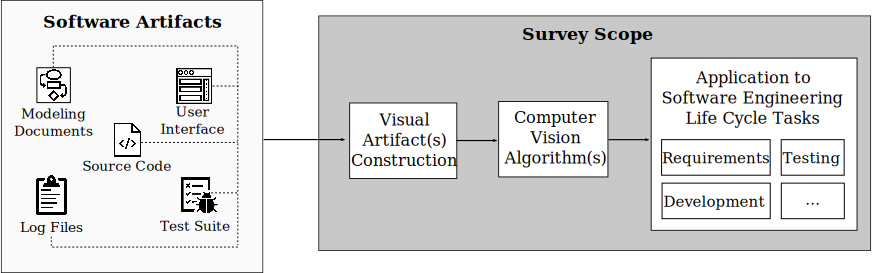
\includegraphics[scale=0.50]{survey/figures/scope-horizontal}
    %}
    \caption{Overview of the scope of this survey.}
    \label{fig:scope}
\end{figure*}





% !TEX root =  manuscript.tex
\section{Methodology}\label{sec:methodology}

In order to conduct the survey in a thorough
and structured manner, we follow the established
guidelines by Kitchenham et al.~\cite{kitchenham2007guidelines}.
We begin by introducing terminology
and concepts needed to understand the remainder
of this survey.
Next, we define the scope of the work
and flesh it out into specific research questions
we aim to answer in this survey.
We then describe the details of the paper
collection process. 
Finally, we specify the inclusion and exclusion criteria
applied to select the most relevant body of work 
from the existing literature. 

\subsection{Definitions}\label{sec:defs}

In order to categorize
the use of visual approaches in software engineering, 
we use the terms \textit{areas} and \textit{tasks}.
Software engineering areas are the various stages in the software
lifecycle~\cite{IEEEComputerSociety:2014:GSE:2616205}.
Examples of SE areas include software requirements, software design,
and software testing.
Within each area, different \textit{tasks} can be defined.
Each task is a specific activity that aims to
achieve a well-defined objective related to that area.
For instance, we refer to unit testing or regression testing as
SE tasks within the software testing SE area,
whereas code migration or code refactoring are tasks within
software maintenance area.
Accordingly, the rationale for using these two terms is
to discuss our findings in more precise levels of granularity,
in order to be able to analyze the findings across areas and
for tasks within a specific area.

Next, we define the following terms in order to clarify
which aspect of computer vision is being discussed:

\begin{defn}[\textbf{Visual Artifact}]
\textit{A visual artifact is any datum %of information 
that satisfies the following two conditions: 
(1)~it constitutes a digital image or video, and
(2)~it is associated with one or more software engineering area(s).}
\end{defn}

\begin{defn}[\textbf{Visual Approach}]
\textit{A visual approach is an algorithm designed to solve a software engineering problem,
which takes as input one or more visual artifacts, 
then typically incorporates a computer vision method or similar techniques as one or more of its steps,
and finally yields an output that is used to achieve a software engineering task.
}
\end{defn}

The rationale for defining these two terms is to have
precision and clarity when describing how visual analysis is used to 
solve a software engineering problem.
We use the term \emph{visual approach} to indicate 
that the approach used to solve an SE problem 
is based on analyzing visual data pertaining to the software.
We use the term \emph{visual artifact} to refer to software artifacts
that are visual in nature, to differentiate them from other
software artifacts that are non-visual (e.g., log files,
requirements documents). 
The link between the two terms is that 
visual artifacts are the visual data consumed
by a visual approach.
Similarly, a visual approach is the algorithm
that needs visual artifacts as input. 
To clarify all of the aforementioned terms,
we give a simple example.  
Consider the case of cross-browser testing,
where the goal is to check whether a given
web app is being rendered identically in different browsers.
Visual approaches for cross-browser testing
often take a screenshot of the app in a set of 
different browsers, and then visually compare the screenshots.
In this case,
screenshots are the visual artifacts used or extracted
from the software,
and screenshot image comparison is the visual approach used to 
solve the SE task of cross-browser testing.

\subsection{Scope}\label{sec:scope}

The scope of this work is to conduct a survey
to help structure, curate, and unify
the dispersed literature in this research area,
and to analyze how computer vision techniques have
been used in software engineering,
and what challenges were reported when they were used. 
This would help shed light on the potential of these 
techniques, and make them more visible and accessible.

\changed{
\autoref{fig:scope} illustrates the scope of this work
in relation to the software engineering life cycle
and other software artifacts. 
The figure should be viewed as a multi-step process, 
beginning with visual artifacts construction, and ending with 
an application to a software engineering task, 
as defined in Section~\ref{sec:defs}.  
As shown in the figure,
the scope is to survey the following aspects: 
(1)~how are visual artifacts (defined in Section~\ref{sec:defs})
constructed or acquired from the software?  
%
This aspect is included in the scope because constructing or acquiring 
visual artifacts is the first step in a computer vision 
processing pipeline, and therefore should be explored 
in order to have a well-rounded survey.
%
(2)~what computer vision algorithms are used to analyze or 
process the constructed visual artifacts? 
% 
This aspect is included in the scope because examining the visual 
processing or analysis conducted in order to address a given paper's 
research questions yields insight into how visual techniques 
can be potentially applied to various tasks of software engineering.
%
(3)~what are the software engineering areas and tasks
where visual approaches have been used?

The figure also helps clarify what areas are outside the scope
of this survey.
For instance, the scope is not concerned with works where 
computer vision techniques were not utilized, 
or works that do not use any visual artifacts. 
Section \ref{sec:inclusions} fleshes out the scope into a detailed set of 
inclusion and exclusion criteria. 
}


\subsection{Research Questions}
As discussed in Section \ref{sec:scope},
the scope is to survey the use of computer vision
in solving software engineering problems.
In this section, we flesh out the scope
into the following specific research questions:

RQ1: What are the main software engineering areas and tasks
for which computer vision approaches have been used to date? 
We formulate this RQ in order to build a high level
picture of the areas of software engineering where computer vision
approaches were used. This aims at identifying potential trends
of areas with high adoption of computer vision 
and conversely areas where little to no computer vision approaches were used.
This can help the software engineering community in identifying
potential gaps in the utilization of computer vision for software engineering. 

RQ2: Why are computer vision approaches adopted? 
We formulate this RQ in order to identify common rationales 
for using computer vision to solve software engineering problems.
This understanding of why computer vision approaches
were used can subsequently help identify new software engineering
areas or tasks where similar problems and rationales exist
and therefore potentially benefiting from computer vision approaches.

RQ3: How are computer vision approaches applied to software and its visual artifacts? 
This RQ is a natural progression of the previous RQs. 
The previous RQs identified the rationales of using computer vision 
and the SE areas where computer vision were used.
This RQ examines the ``how.''
That is, the mechanism(s) by which computer vision was applied to software.
This can help guide the implementation of computer vision approaches
to solve software engineering problems.

RQ4: How are software engineering tasks that leverage computer vision techniques evaluated? 
This RQ examines the methods used to evaluate the use of computer vision approaches
in software engineering problems, as well as a summary of the reported limitations and challenges.
This may help with selecting an evaluation strategy when exploring the use of a computer vision approach,
and informing adopters of potential challenges.

\begin{figure*}
    \centering
    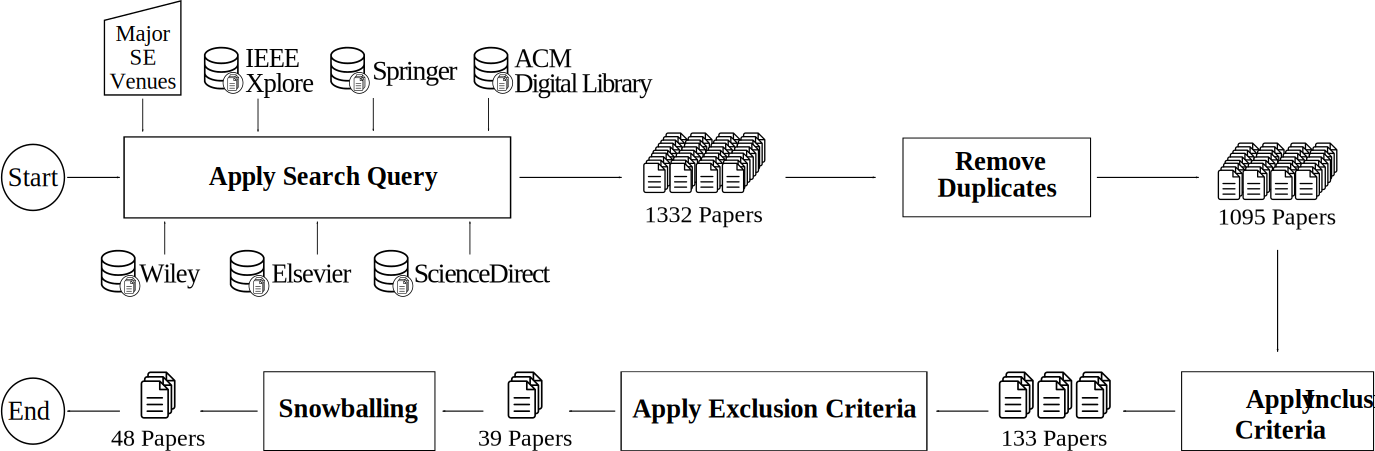
\includegraphics[width=0.80\textwidth]{survey/figures/overview}
    \caption{Overview of the paper collection process. }
    \label{fig:overview}
\end{figure*}

\subsection{Paper Collection}\label{sec:collection}

\autoref{fig:overview} shows our paper search and selection process.
In order to collect as much relevant literature as possible, 
we used two types of sources for paper collection: 
paper repository databases, and major software engineering venues.

\header{Paper Repository Databases}
To conduct our search, we used the databases of the following
well-known publishers of scientific literature:
IEEE Xplore, ACM Digital Library, ScienceDirect, Springer, Wiley, and Elsevier.
The search covers papers that have been published until June 2020. 
We used more than one database to ensure collecting
as many papers as possible from all known publishers.

\header{Software Engineering Venues}
The preceding selection of paper repositories
aims at casting a wide net in order to capture as many
relevant literature as possible.
However, since the databases contain an extremely large
number of papers, it is possible that papers 
relevant to our survey are lost in the vast number of returned papers.

For this reason, and in order to make sure we collect highly relevant papers, we complemented the database search with a manual issue-by-issue search within the conference proceedings and journal articles from 
top-tier software engineering venues (listed in \autoref{tbl:paper-sources}).
The final pool of collected papers is the combined list of papers from both the database search and the SE venues search.

\changed{
\header{Interdisciplinary Venues}
Given the interdisciplinary nature of this work, 
we also performed manual issue-by-issue search within 
the conference proceedings of relevant fields, namely, 
computer-human interaction, computer vision and machine 
learning. We selected the top three venues (based on the h5 index from Google Scholar) from each field.
The searched venues are listed in the last section of
 \autoref{tbl:paper-sources} (under ``Interdisciplinary Venues'').
}

\header{Search Query} For each of the aforementioned sources, 
we performed a search query using various combinations
of terms to retrieve papers in different software engineering areas
that are potentially using computer vision.
The query was performed on all data fields of the paper,
returning matches to either the \emph{title}, \emph{abstract},
\emph{keywords}, or \emph{text} of the paper.
The query is composed of two parts: keywords related to the approach
and keywords of the various software engineering areas.
Keywords of the approach include strings such as
``computer vision'' or ``visual''.
They were included in the query in order to indicate
our interest in works that use computer vision or visual approach.
Keywords describing the areas include strings such as
``development'' or ``testing'' or any of the software engineering
life cycle phases (e.g., requirements, maintenance).
The final applied search query is as follows:
%\begin{quote}
\emph{{[}computer vision {OR} image processing 
{OR} image analysis {OR} visual{]}
\ \ {AND}\ \ 
{[}requirements {OR} design {OR} development 
{OR} testing {OR} maintenance {OR} comprehension {]}}
%\end{quote}
The result of this query led to an initial pool of \initialPoolSize papers,
which was further filtered in the next stages.

\header{Duplicates removal}
During the paper collection step, we aimed to be
thorough by including as many paper sources as possible
in order to capture all potentially relevant works.
However, this resulted in many duplicate papers since a given
paper might be included in more than one database and venue.
Therefore, we filtered the collected pool
of papers by removing duplicate works based on their titles.

\subsubsection{Inclusion and Exclusion Criteria}\label{sec:inclusions} 
The search conducted on the databases and venues is, 
by design, very inclusive. This allows us to collect as many
papers as possible in our pool. 
However, this generous inclusivity results in having papers that are not directly
related to the scope of this survey.
Accordingly, we define a set of specific inclusion and exclusion criteria
and apply them to each paper in the pool, and remove papers not meeting the criteria.
This ensures that each collected paper is inline with our scope and research questions.

\header{Inclusion criteria}
We define the following inclusion criteria: 
%
(1)~The paper should be contributing to any stage
of the software engineering process,
whether in early requirements and modeling,
through development and design, or finally testing and maintenance.
We included this criteria in order to focus on software engineering papers.
This is because we found a notable number of computer vision papers 
that were in fields other than software engineering (e.g., biology).
%
(2)~The paper should include a computer vision processing of the software or its artifacts.
That is, the work achieves its objective (whether partially or fully) by extracting,
analyzing, or processing visual artifacts pertaining or relevant to the software.
This is an important and key criterion for paper selection because it ensures
we meet the core scope of our survey. 
%
(3)~The paper should be a full technical research paper that has a
detailed description of the visual approach utilized.
This criterion is imposed in order to have sufficient information to answer our research questions.
Answering our research questions, such as RQ3 and RQ4, requires that 
we examine technical software engineering research papers,
as opposed to, for instance,
technical magazine articles, industrial white papers, or similar grey literature
which do not have sufficient level of detail.
Some demo/short papers can be allowed if they have dedicated and detailed 
sections discussing the detailed mechanism of the visual approach and its
evaluation. 
This enables creating a pool of papers that have
rich and detailed information and findings,
in order to answer key research questions related to
the details of the visual approach, the process of creating visual artifacts,
and evaluation strategies. 
%
(4)~The paper should contain a section dedicated to illustrating
some form of quantitative or qualitative evaluation of the technique,
or an illustration of its use case. 
This criterion was imposed in order to enable us to
fully answer and explore our research questions regarding evaluation strategies.

These criteria were applied 
in a group review process by the authors.
For each paper in the pool, each author initially checked the title and abstract,
and briefly examined the proposed approach and results to ensure that it meets the inclusion criteria.
If this check was not sufficient to conclusively decide
whether the paper should be included in the pool,
we proceeded with a secondary in-depth examination of
the paper's objective, methodology, and evaluation to ensure that the inclusion criteria were met.
Finally, a discussion among the authors was triggered,
to decide on the inclusion of the paper in the final list of works.
 
% !TEX root =  manuscript.tex

\begin{table}

\revised{0.99\textwidth}{

\caption{Conference proceedings and journals considered for paper collection (in addition to database search).}
\centering
% \small % bigger
\scriptsize %smaller
% \tiny % much smaller
\renewcommand{\arraystretch}{1.2}
\setlength{\tabcolsep}{2.5pt}

\begin{tabular}{l l p{7.5cm}}
	\toprule
	& \textbf{Acronym}   & \textbf{Venue}                                                                                              \\ \midrule
	\multirow{18}{*}{\rotatebox{90}{\textbf{SE Conferences}}}
	& ICSE          & International Conference on Software Engineering                                                            \\
	& FSE           & International Symposium on Foundations of Software Engineering                                  \\
	& ESEC/FSE	    & Joint European Software Engineering Conference and Symposium on the Foundations of Software Engineering \\
	& ASE           & International Conference on Automated Software Engineering                                         \\
	& ESEM          & International Symposium on Empirical Software Engineering and Measurement                         \\
	& ICST          & International Conference on Software Testing, Verification and Validation                              \\
	& ISSTA         & International Symposium on Software Testing and Analysis                                        \\
	& MSR           & International Conference on Mining Software Repositories                                                    \\
	& RE            & International Requirements Engineering Conference                                                      \\
	& ICSME         & International Conference on Software Maintenance and Evolution                                          \\
	& MODELS        & International Conference on Model Driven Engineering Languages and Systems                         \\
	& ISSRE         & International Symposium on Software Reliability Engineering                                            \\
	& EASE          & Evaluation and Assessment in Software Engineering                                                           \\
	% & UIST          & ACM Symposium on User Interface Software and Technology                                                     \\
	% & WWW           & International World Wide Web conference                                                                     \\
	% & WSDM          & ACM International Conference on Web Search and Data Mining                                                  \\
	% & ICWE          & International Conference on Web Engineering                                                                 \\
	% & CHI           & ACM CHI Conference on Human Factors in Computing Systems                                                    \\ \midrule
	\midrule
	\multirow{12}{*}{\rotatebox{90}{\textbf{SE Journals}}}
	& TSE           & Transactions on Software Engineering                                                                   \\
	& EMSE          & Empirical Software Engineering                                                                              \\
	& TOSEM         & Transactions on Software Engineering and Methodology                                                    \\
	& JSS           & Journal of Systems and Software                                                                             \\
	% & JVLC          & Journal of Visual Languages and Computing                                                                   \\
	& JSEP          & Journal of Software: Evolution and Process                                                                  \\
	& STVR          & Software Testing, Verification and Reliability                                                              \\
	& ASE           & Automated Software Engineering                                                                              \\
	& IEEE SOFTWARE & IEEE Software                                                                                               \\
	& IET SOFTW.    & IET Software                                                                                                \\
	& IST           & Information and Software Technology                                                                         \\
	& SQJ           & Software Quality Journal                                                                                    \\ 


	\midrule
	
	\multirow{10}{*}{\rotatebox{90}{\textbf{Interdisciplinary Venues}}}
	& CHI       & Conference on Human Factors in Computing Systems  	\\
	& CSCW 		& Conference on Computer-Supported Cooperative Work 	\\
	& UbiComp	& Conference on Pervasive and Ubiquitous Computing 		\\ 
	& UIST      & Symposium on User Interface Software and Technology  	\\

	& NeurIPS   & Conference on Neural Information Processing Systems   \\
	& ICLR		& International Conference on Learning Representations  \\
	& ICML		& International Conference on Machine Learning			\\

	& CVPR    & Conference on Computer Vision and Pattern Recognition   \\
	& ECCV	  & European Conference on Computer Vision					\\
	& ICCV		& International Conference on Computer Vision		\\
	
	\bottomrule

	\end{tabular}
	\label{tbl:paper-sources}
}
\end{table}


\header{Exclusion criteria}\label{sec:exclusions}
During our initial experimental test rounds of paper searching,
we observed that a relatively large number of retrieved papers
were on visualization research.
This is understandable and expected because our queries
include terms such as image, visual, and design.

Accordingly, we exclude papers published in the area of software
visualization for the following reasons.
First, the visualization class of algorithms does not
constitute a \emph{visual approach}, as defined in Section~\ref{sec:defs}.
Visualizations do not use any visual artifact of the software \emph{as an input}.
Rather, such work performs a final visual output or visual
representation of a complete, non-visual, approach.
Accordingly, this area of research is excluded
since it would be outside the scope of this work.
We recall that the scope is to survey visual approaches which,
by definition, \emph{consume} visual artifacts pertaining to the software during the
course of running their algorithm or processing.
Second, in addition to visualization being outside the scope of this survey,
it is already a well-known and common aspect of software engineering, 
and plenty of surveys already exist on the use of visualization
in various aspects of software engineering, 
as mentioned in \Cref{sec:related}.

We also exclude commercial software services or open-source tools
that have no corresponding publication, for the following reasons.
First, including services or tools that are not peer-reviewed
would negatively impact our ability to conduct the survey because tools and services 
that are not backed by a publication do not include
a detailed explanation of their approach.
This reduces our ability to answer key research questions for this survey,
such as what specific computer vision techniques were used,
what is the visual artifacts construction process, and 
how were the computer vision algorithms applied to the visual artifacts.
Services and tools without a corresponding publication
also typically do not have a thorough systematic evaluation,
and therefore we are unable to answer research questions related to
how computer vision techniques were evaluated,
what are the main findings, and what were the challenges.


\header{Snowballing}
At the end of searching database repositories and
conference proceedings and journals,
and applying inclusion and exclusion criteria,
we obtained a total of 57 unique papers.
Next, 
to mitigate the risk of omitting relevant literature from this survey,
we also performed backward snowballing~\cite{Wohlin:2014:GSS:2601248.2601268}
by inspecting the references cited by the collected papers so far.
Nine additional papers were retrieved during this phase,
which led to a final pool of 66 unique papers.
\autoref{table:selected-primary-studies}
shows the final pool of papers
that will be discussed and analyzed in the remainder of this work.

% !TEX root =  manuscript.tex

\begin{table}[t]
\caption{Collected data items (Synthesis Matrix)}
\centering
\renewcommand{\arraystretch}{1.2}
\setlength{\tabcolsep}{9pt}
\begin{tabular}{l l}
	\toprule
	\textbf{Field}                    & \textbf{Use}     \\ \midrule
	Title                             & Documentation    \\
	Author(s)                         & Documentation    \\
	DOI identification number         & Documentation   \\
	Abstract                          & Paper Selection \\
	Text                          & Paper Selection \\
	Venue                             & RQ1             \\
	Year                              & RQ1             \\
	% Total number of Citations         & \davood{?}      \\
	Target platform                   & RQ1             \\
	Software engineering area         & RQ1             \\
	Software engineering task         & RQ1             \\
	Reasons for adopting CV approach  & RQ2             \\
	Visual artifact(s) used           & RQ3             \\
	CV algorithm(s) used    	      & RQ3             \\
	Evaluation process \& challenges  & RQ4             \\
	Main results                      & RQ4             \\
	Limitations of CV methods used    & RQ4             \\ \bottomrule
\end{tabular}
	\label{tbl:collected-info}
\end{table}


\header{Extracted Information}
For each retrieved paper,
we collect a set of data necessary to answer the research questions. 
\autoref{tbl:collected-info} shows the list of data
collected from each paper
and their mapping to each research question.
As shown in the table,
the title, author(s), and document ID were used
for documentation purposes to keep track of the various papers.
The abstract and text were used for the paper selection process
and applying the inclusion and exclusion criteria.
The venue, year, software engineering area and task
of each paper was also collected in order to discuss and answer
RQ1. 
We also extract the target platform for each paper, which is  
the type of computing device (e.g., desktop, mobile) that the 
analyzed software runs on.
A list of reasons for adopting computer vision was also 
extracted from each paper in order to answer RQ2.
The visual artifact(s) and the visual approach utilized
were also identified in each paper in order to discuss RQ3.
Finally, we log the evaluation process and the results and findings
from each collected paper in order to answer RQ4.
All these data are collected, analyzed, and used to synthesize 
the findings for the rest of this survey. 
In order to facilitate the use of this data by
the general research community, the data have been 
made publicly available at http://tiny.cc/tse-2020.

% !TEX root =  manuscript.tex
\begin{sidewaystable}
%\begin{table*}
%\scriptsize
\tiny
\renewcommand{\arraystretch}{1.0}
\setlength{\tabcolsep}{4.5pt}
%\revised{1.01\textwidth}{
\caption{Collected pool of papers (in chronological order).}
\label{table:selected-primary-studies}
\begin{tabular}{@{} lp{12.9cm}ll @{}}
%\begin{longtable}{@{} lp{12.9cm}ll @{}}
\toprule
\textbf{Reference}           & \textbf{Title}                                                                                                                      & \textbf{Venue} & \textbf{Year} \\  

\midrule

% \rowcolor{\hlcolor}
\citet{Landay-2001-IEEEComputer}       & Sketching Interfaces: Toward More Human Interface Design                                                                  & IEEE Computer  & 2001          \\
\citet{Caetano-2002-AAAI}    & JavaSketchIt: Issues in Sketching The Look of User Interfaces                                                                       & AAAI           & 2002          \\
% \rowcolor{\hlcolor}
\citet{Fails-2003-CHI}       & A Design Tool for Camera-based Interaction                                                                                          & CHI            & 2003          \\

\citet{Coyette-2007-INTERACT}& Multi-fidelity Prototyping of User Interfaces                                                                                       & INTERACT       & 2007          \\

% \rowcolor{\hlcolor}
\citet{Zheng-2009-CHI}       & Correlating Low-level Image Statistics with Users - Rapid Aesthetic and Affective Judgments of Web Pages                            & CHI            & 2009          \\
\citet{Chang-2010-CHI}       & GUI Testing Using Computer Vision                                                                                                   & CHI            & 2010          \\
\citet{Choudhary-2010-ICSM}  & WEBDIFF: Automated Identification of Cross-browser Issues in Web Applications                                                       & ICSM           & 2010          \\
\citet{Li-2010-CHI}          & FrameWire: A Tool for Automatically Extracting Interaction Logic from Paper Prototyping Tests                                       & CHI            & 2010          \\
% \rowcolor{\hlcolor}
\citet{Dixon-2010-CHI}       & Prefab: Implementing Advanced Behaviors using Pixel-based Reverse Engineering of Interface Structure                                & CHI            & 2010          \\

\citet{Delamaro-2011-STVR}   & Using Concepts of Content‐based Image Retrieval to Implement Graphical Testing Oracles                                              & STVR           & 2011          \\
\citet{Dixon-2011-CHI}       & Content and Hierarchy in Pixel-based Methods for Reverse Engineering Interface Structure                                            & CHI            & 2011          \\
\citet{Seifert-2011-MobileHCI} & Mobidev: A Tool for Creating Apps on Mobile Phones                                                                                & MobileHCI      & 2011          \\
\citet{Choudhary-2012-ICST}  & Crosscheck: Combining Crawling and Differencing to Better Detect Cross-browser Incompatibilities in Web Applications                & ICST           & 2012          \\

% \rowcolor{\hlcolor}
\citet{Givens-2013-ICSE}     & Exploring The Internal State of User Interfaces by Combining Computer Vision Techniques with Grammatical Inference                  & ICSE           & 2013          \\

% \rowcolor{\hlcolor}
\citet{Liang-2013-UIST}      & SeeSS: Seeing What I Broke -- Visualizing Change Impact of Cascading Style Sheets (CSS)                                             & UIST           & 2013          \\


\citet{Scharf-2013-ICSE}     & Dynamic Injection of Sketching Features Into GEF-based Diagram Editors                                                              & ICSE           & 2013          \\
\citet{Alegroth-2013-ICST}   & JAutomate: A Tool for System- and Acceptance-test Automation                                                                        & ICST           & 2013          \\
\citet{Semenenko-2013-ICSM}  & Browserbite: Accurate Cross-Browser Testing via Machine Learning over Image Features                                                & ICSM           & 2013          \\
\citet{Choudhary-2013-ICSE}  & X-PERT: Accurate Identification of Cross-Browser Issues in Web Applications                                                         & ICSE           & 2013          \\
\citet{Lin-2014-TSE}         & On the Accuracy, Efficiency, and Reusability of Automated Test Oracles for Android Devices                                          & TSE            & 2014          \\
\citet{Mahajan-2014-ASE}     & Finding HTML Presentation Failures Using Image Comparison Techniques                                                                & ASE            & 2014          \\
\citet{Amalfitano-2014-WISE} & Towards Automatic Model-in-the-loop Testing of Electronic Vehicle Information Centers                                               & WISE           & 2014          \\
\citet{Selay-2014-DICTA}     & Adaptive Random Testing for Image Comparison in Regression Web Testing                                                              & DICTA          & 2014          \\

% \rowcolor{\hlcolor}
\citet{Bao-2015-ICSE}        & scvRipper: Video Scraping Tool for Modeling Developers' Behavior Using Interaction Data                                             & ICSE           & 2015          \\

\citet{Nguyen-2015-ASE}      & Reverse Engineering Mobile Application User Interfaces with REMAUI                                                                  & ASE            & 2015          \\
\citet{Burg-2015-UIST}       & Explaining Visual Changes in Web Interfaces                                                                                         & UIST           & 2015          \\
\citet{Mahajan-2015-ICST}    & Detection and Localization of HTML Presentation Failures Using Computer Vision-Based Techniques                                     & ICST           & 2015          \\
\citet{Hori-2015-SEKE}       & An Oracle based on Image Comparison for Regression Testing of Web Applications                                                      & SEKE           & 2015          \\

% \rowcolor{\hlcolor}
\citet{Reinecke-2016-CHI}    & Enabling Designers to Foresee Which Colors Users Cannot See                                                                         & CHI            & 2016          \\

\citet{Deka-2016-UIST}       & ERICA: Interaction Mining Mobile Apps                                                                                               & UIST           & 2016          \\
\citet{Ponzanelli-2016-ICSE} & Too Long; Didn’t Watch! Extracting Relevant Fragments from Software Development Video Tutorials                                     & ICSE           & 2016          \\
\citet{Mahajan-2016-ICST}    & Using Visual Symptoms for Debugging Presentation Failures in Web Applications                                                       & ICST           & 2016          \\
\citet{Feng-2016-ASE}        & Multi-objective Test Report Prioritization Using Image Understanding                                                                & ASE            & 2016          \\
\citet{Patric-2016-ASE}      & Automatic Test Image Generation Using Procedural Noise                                                                              & ASE            & 2016          \\
\citet{He-2016-ICWS}         & X-Check: A Novel Cross-browser Testing Service Based on Record/Replay                                                               & ICWS           & 2016          \\

\citet{Deka-2017-UIST}       & Rico: A Mobile App Dataset for Building Data-Driven Design Applications                                                             & UIST           & 2017          \\
\citet{Wan-2017-STVR}        & Detecting Display Energy Hotspots in Android Apps                                                                                   & STVR           & 2017          \\
\citet{Bao-2017-EMSE}        & Extracting and Analyzing Time-series HCI Data from Screen-captured Task Videos                                                      & EMSE           & 2017          \\
\citet{Zhang-2017-ASE}       & Sketch-guided GUI Test Generation for Mobile Applications                                                                           & ASE            & 2017          \\
\citet{Chen-2017-IUI}        & UI X-Ray: Interactive Mobile UI Testing Based on Computer Vision                                                                    & IUI            & 2017          \\

% \rowcolor{\hlcolor}
\citet{Wu-2017-CSCW}         & Automatic Alt-text: Computer-generated Image Descriptions for Blind Users on a Social Network Service                               & CSCW           & 2017          \\


\citet{Reiss-2018-ASEj}      & Seeking the User Interface                                                                                                          & ASE J.         & 2018          \\
\citet{Kirac-2018-JSS}       & VISOR: A Fast Image Processing Pipeline with Scaling and Translation Invariance for Test Oracle Automation of Visual Output Systems & JSS            & 2018          \\
\citet{Leotta-2018-STVR}     & Pesto: Automated Migration of DOM‐based Web Tests Towards the Visual Approach                                                       & STVR           & 2018          \\
\citet{canvas_icst2018}   & Web Canvas Testing through Visual Inference                                                                                         & ICST           & 2018          \\
\citet{Xu-2018-TOIT}         & Cross-Browser Differences Detection Based on an Empirical Metric for Web Page Visual Similarity                                     & TOIT           & 2018          \\
\citet{Kuchta-2018-EMSE}     & On the Correctness of Electronic Documents: Studying, Finding, and Localizing Inconsistency Bugs in PDF Readers and Files           & EMSE           & 2018          \\
\citet{Bao-2018-TSE}         & VT-Revolution: Interactive Programming Video Tutorial Authoring and Watching System                                                 & TSE            & 2018          \\
\citet{Moran-ICSE-2018}      & Automated Reporting of GUI Design Violations for Mobile Apps                                                                        & ICSE           & 2018          \\

% \rowcolor{\hlcolor}
\citet{Chen-2018-ICSE}       & From UI Design Image to GUI Skeleton: A Neural Machine Translator to Bootstrap Mobile GUI Implementation                            & ICSE           & 2018          \\

% \rowcolor{\hlcolor}
\citet{Sun-2018-ICML}        & Neural Program Synthesis from Diverse Demonstration Videos                                                                          & ICML           & 2018          \\

% \rowcolor{\hlcolor}
\citet{Lim-2018-UIST}        & Ply: A Visual Web Inspector for Learning from Professional Webpages                                                                 & UIST           & 2018          \\

\citet{Moran-TSE-2018}       & Machine Learning-Based Prototyping of Graphical User Interfaces for Mobile Apps                                                     & TSE            & 2018          \\
\citet{Stocco-2018-FSE}      & Visual Web Test Repair                                                                                                              & FSE            & 2018          \\
\citet{Tanno-2018-ICSTW}     & Support for Finding Presentation Failures by Using Computer Vision Techniques                                                       & ICST           & 2018          \\
\citet{bajammal2018generating}    & Generating Reusable Web Components from Mockups                                                                                     & ASE            & 2018          \\
\citet{Moran-2018-ASE}       & Detecting and Summarizing GUI Changes in Evolving Mobile Apps                                                                       & ASE            & 2018          \\
\citet{Natarajan-2018-MOBILESoft} & P2A: A Tool for Converting Pixels to Animated Mobile Application User Interfaces                                               & MOBILESoft     & 2018          \\
\citet{Osman-2018-SEAA}      & An Automated Approach for Classifying Reverse-engineered and Forward-engineered UML Class Diagrams                                  & SEAA           & 2018          \\
\citet{Xiao-2019-ICSE}       & Automatic Identification of Sensitive UI Widgets based on Icon Classification for Android Apps                                      & ICSE           & 2019          \\ 
\citet{Huang-2019-CHI}       & Swire: Sketch-based User Interface Retrieval                                                                                        & CHI            & 2019          \\

% \rowcolor{\hlcolor}
\citet{Zhao-2019-ICSE}       & ActionNet: Vision-Based Workflow Action Recognition from Programming Screencasts                                                    & ICSE           & 2019          \\

% \rowcolor{\hlcolor}
\citet{Yu-2019-ASE}          & LIRAT: Layout and Image Recognition Driving Automated Mobile Testing of Cross-Platform                                              & ASE            & 2019          \\

% \rowcolor{\hlcolor}
\citet{Swearngin-2019-CHI}   & Modeling Mobile Interface Tappability using Crowdsourcing and Deep Learning                                                         & CHI            & 2019          \\

% \rowcolor{\hlcolor}
\citet{Yuan-2020-CHI}        & Modeling Human Visual Search Performance on Realistic Webpages using Analytical and Deep Learning Methods                           & CHI            & 2020          \\

% \rowcolor{\hlcolor}
\citet{Wu-2020-CHI}          & Predicting and Diagnosing User Engagement with Mobile UI Animation via a Data-Driven Approach                                       & CHI            & 2020          \\ 

\bottomrule 

%\end{longtable}
\end{tabular}
%}
%\end{table*}
\end{sidewaystable}

% !TEX root =  manuscript.tex
\section{Findings}\label{sec:results}

% !TEX root =  manuscript.tex
\subsection{Trends and Landscape}\label{sec:trends}

\begin{figure}%[b]
	\revised{\linewidth}{
		\centering
		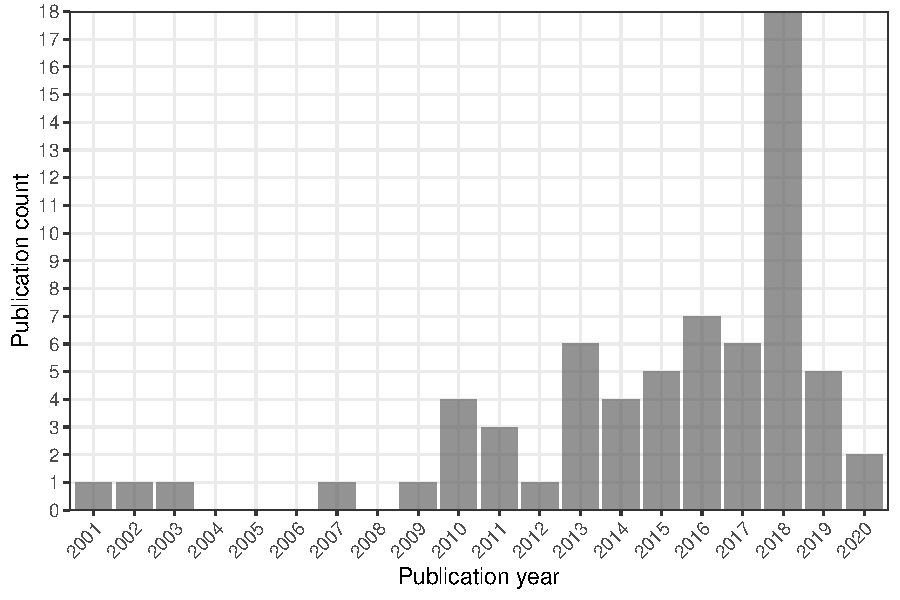
\includegraphics[width=0.85\textwidth]{survey/figures/years-publications}
		\caption{Distribution of publications across years. }
		\label{fig:years-publications}
	}
\end{figure}


\changed{
At the end of the paper collection process,
we obtained a pool of papers spanning the years 2001-2020 (June 2020).
\autoref{table:selected-primary-studies} shows
the final list of \numberOfPapers papers.
\autoref{fig:years-publications} shows the distribution of
the retrieved pool of papers across different years of publication.
Overall, we observed a generally increasing long-term trend in
the use of computer vision approaches in software engineering. 
This research area is also relatively new, 
with more than half of the papers in our pool 
published in the past five years.
Furthermore, \autoref{fig:areas-trend} depicts the cumulative number of publications 
per software engineering area across different years.
The results indicate that software testing is the area 
exhibiting the most rapid increase
in terms of the number of publications 
wherein a computer vision technique is utilized.
}




\begin{figure}
\revised{\linewidth}{
\centering
%\fbox{
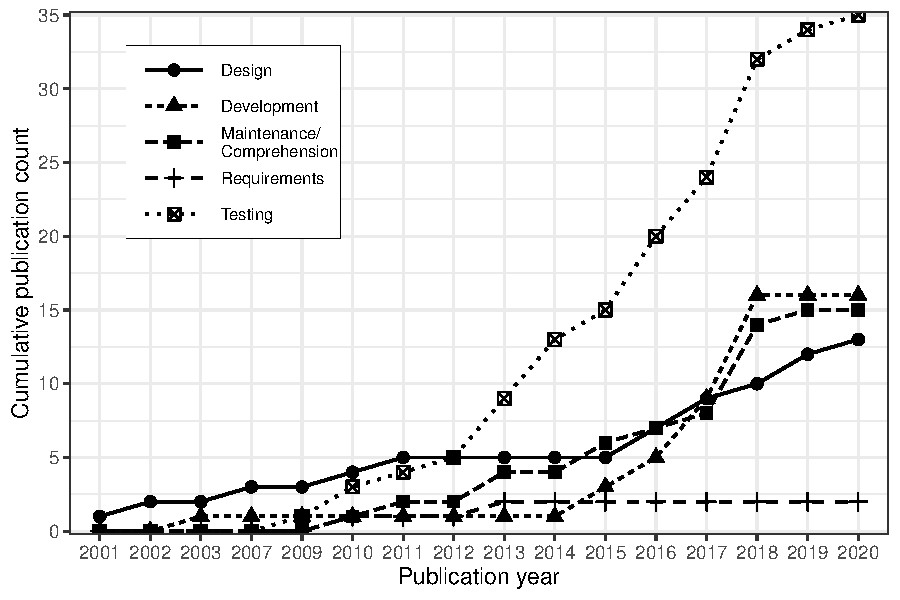
\includegraphics[width=\linewidth]{survey/figures/areas-trend-cumulative}
%}
\caption{Cumulative distribution of publications across years per SE area.
Testing is the most common area, followed by development and maintenance.} \label{fig:areas-trend} 
}
\end{figure}

\changed{
\autoref{fig:venues-publications} shows the distribution 
of the published papers across venues.
The main venues in which computer vision approaches 
for software engineering were published are 
the Conference on Human Factors in Computing Systems (CHI) with 11 papers, 
the International Conference on Software Engineering (ICSE) with nine papers, 
and the International Conference on Automated Software Engineering (ASE) with eight papers. 
The presence of traditional SE venues as well as venues from other fields (e.g. CHI) 
in \autoref{fig:venues-publications} provides some indication that 
research on the use of computer vision for software engineering tasks 
is an interdisciplinary field. 
}


\subsection{Areas, Tasks, and Platforms (RQ1)}\label{sec:rq1}

\begin{figure}%[b]
	\revised{\linewidth}{
		\centering
		%\fbox{
		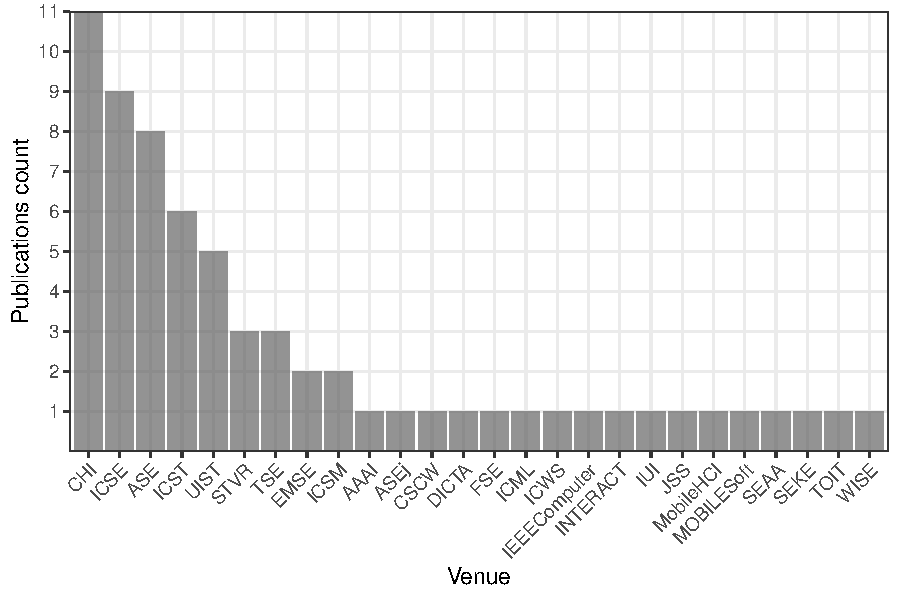
\includegraphics[width=\linewidth]{survey/figures/venues-publications}
		%}
		\caption{Distribution of the publications across venues. }\label{fig:venues-publications}
	}
\end{figure}

To study the exiting applications of visual techniques for SE,
we analyzed the selected papers to find out
which \textit{SE areas} have been explored,
for which \textit{tasks}, and on which \textit{platforms} they were used.
As defined in section \ref{sec:defs}, SE areas are high-level stages
of the software engineering life cycle,
such as requirements, testing, or development.
SE tasks are more fine-grained activities, such as unit testing or regression testing.
The platforms are the types of computing devices (e.g., desktop, mobile) 
that the analyzed software runs on. 
We further looked into the papers' discussion sections to gain insights from
the authors about other areas in which the proposed technique could potentially be applied.

\subsubsection{Software Engineering Areas and Tasks}

\autoref{fig:software-engineering-tasks}
presents the papers distribution across different SE areas and tasks.
Note that the number of papers indicated in the figure
is more than the total number of papers in the pool.
This is due to the fact that for some papers, the presented approach can be utilized for more than one task.
We now discuss more in detail the trends of \autoref{fig:software-engineering-tasks}.

\begin{figure}
    \revised{\linewidth}{
\centering
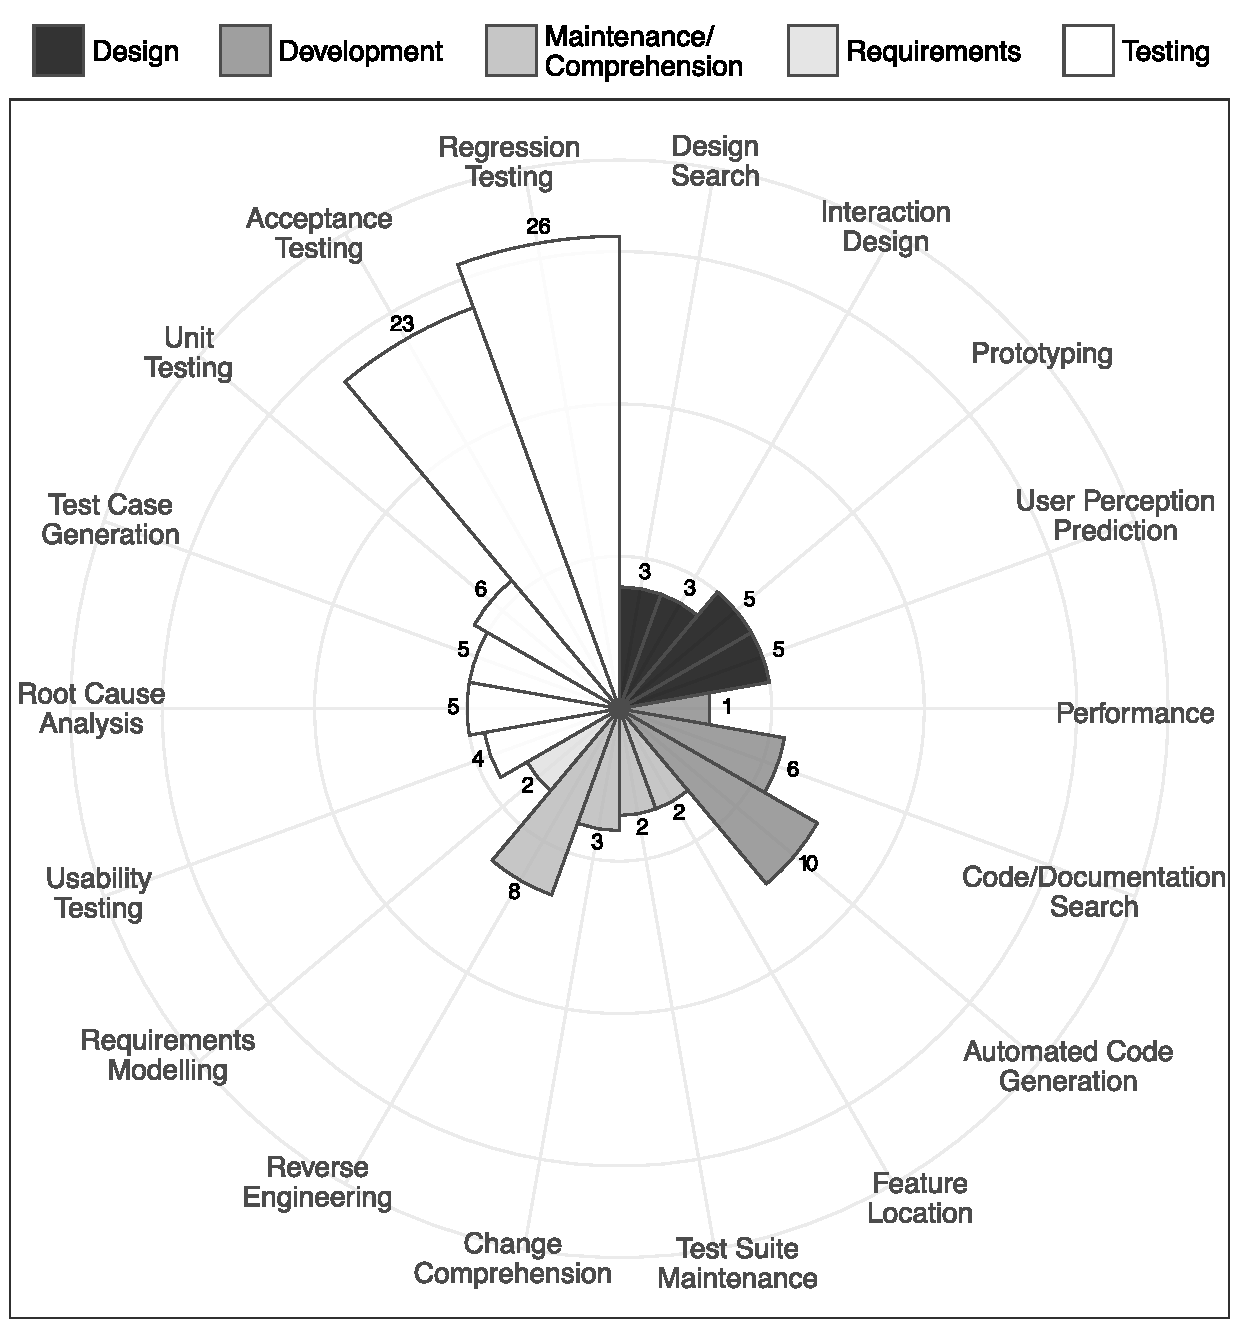
\includegraphics[width=0.8\linewidth]{survey/figures/areas}
\caption{Papers distribution across different Software Engineering Areas and Tasks}
\label{fig:software-engineering-tasks}
    }
\end{figure}


\header{Testing}
Software testing is the most common research area 
for which approaches using computer vision are proposed, 
accounting for approximately half of all collected papers.
A closer look at the publications in this area reveals interesting trends. 
\textbf{Regression Testing.} Most of the studies use visual methods to facilitate acceptance and regression testing e.g., by 
comparing visual artifacts (e.g., the GUIs) 
with each other or with respect to a given oracle.
Without adopting computer vision, developers would most 
likely need to perform some kind of manual evaluation, 
e.g., through eyeball analysis to spot deviations from 
the expected visual presentation---a daunting and error-prone task.
Apart from GUI comparisons, computer vision (CV) techniques have been also utilized 
for other software testing tasks.
%
For example,
%
\citet{Kuchta-2018-EMSE} introduce a technique for regression 
testing of PDF reader software and localizing faulty parts of PDF files.
The adopted technique exploits \textit{differential testing}, 
where the (visual) output of multiple implementations of a 
program---the PDF viewer---is compared to the same input to spot deviations.
%
In another work, \citet{Leotta-2018-STVR} propose an automated 
code migration tool for automatically converting end-to-end 
Selenium web tests to visual web tests based on 
Sikuli's~\cite{Chang-2010-CHI} image recognition capabilities.
%
\citet{Kirac-2018-JSS} provide an image comparison technique 
for black-box, regression testing of visual-output software 
used in consumer electronics.
The approach removes noise to eliminate image differences 
caused by scaling and translation, and is evaluated on the output of digital TVs.
%
\citet{canvas_icst2018} propose a technique to test 
state-free canvas elements on web pages by reverse-engineering a visual model.
This allows unit testing of the specific visual elements contained in the canvas.


\textbf{Cross-browser Testing}. A significant class of software testing techniques leveraging visual methods aims at automatically identifying \textit{cross-browser incompatibilities} (XBIs) for web 
applications~\cite{Choudhary-2010-ICSM, Choudhary-2012-ICST,
Semenenko-2013-ICSM, Choudhary-2013-ICSE, Selay-2014-DICTA, He-2016-ICWS, Xu-2018-TOIT}.
XBIs are frequently-occurring issues in web pages' 
appearance and/or behavior when the same page is viewed 
on different web browsers~\cite{Choudhary-2013-ICSE}.
Identifying such differences requires laborious human judgement,
which can be effectively reduced using an automated visual-based technique.
A recent literature review by \citet{Sabaren-2018-JCST} 
surveys the techniques proposed to tackle XBIs.

A similar problem involves using visual methods for 
\textit{root cause analysis} of presentational issues 
occurring on web pages~\cite{Mahajan-2014-ASE, Mahajan-2015-ICST,
Mahajan-2016-ICST}.
In addition to the web domain, root cause analysis 
is also used to identify rendering issues in PDF 
files~\cite{Kuchta-2018-EMSE}, as well as, the causes
of excessive energy consumption of UIs in mobile 
applications~\cite{Wan-2017-STVR}.

Several approaches attempt to automate test 
execution using visual techniques. An example 
is \textit{record-and-replay testing} where the 
screenshots of the GUI and the human tester's 
actions and inputs performed on the GUI are recorded~\cite{Chang-2010-CHI,
Alegroth-2013-ICST, Lin-2014-TSE, He-2016-ICWS} . 
Popular visual record-and-replay tools are 
Sikuli~\cite{Chang-2010-CHI} and 
JAutomate~\cite{Alegroth-2013-ICST}, which allow 
fast and easy replay of the same sequence of actions:
the tool conducts a visual search on the current 
visible contents of the screen to detect the 
widgets' locations, triggers the recorded 
actions and inputs, and finally performs a visual assertion,
comparing the observed visual outcome with the expected oracle.

Besides record-and-replay tools, test automation with 
visual analysis has been successfully applied to 
\textit{automotive software engineering}. 
\citet{Amalfitano-2014-WISE} propose a tool to automate 
the testing of the emulated vehicle information 
systems' panels.
The testers can locate visual elements on the panel 
and specify their properties; the tool allows to 
check the panel's output with respect to these 
properties at pre-defined timestamps.

\changed{
\citet{Zheng-2009-CHI}, \citet{Yuan-2020-CHI}, 
\citet{Deka-2016-UIST}, and \citet{Deka-2017-UIST} 
aim to automate the testing of \textit{aesthetics 
or usability} of web pages. 
This line of work involves building computer vision 
models that can predict whether web pages 
meet certain aesthetic requirements pertaining to 
the usability of a page (e.g. visual balance of 
white space and elements, consistent and simple 
representation of elements on a web page).
}

\citet{Patric-2016-ASE} propose an approach based 
on systematic image manipulation to \textit{automatically 
generate test input images} for regression and 
acceptance testing of an epidemiological simulation software.
The software's output on these input images is 
monitored and unexpected deviations reveal bugs or regressions in the code.

To \textit{prioritize test reports}, \citet{Feng-2016-ASE} 
use the screenshots provided by users to augment the 
existing textual test prioritization techniques for mobile applications. 
Finally, to \textit{automatically generate test cases}, 
\citet{Zhang-2017-ASE} use a visual-aided approach
that identifies strokes that testers draw on 
screenshots taken from the apps. These sketches are 
used to define test specifications (e.g., coordinates 
where a visual object should be positioned to on 
the screen), which are subsequently used to 
generate test cases automatically.

\header{Design}
\changed{
Our survey included a number of papers aiming at 
facilitating the design stage of software systems 
by means of computer vision. 
\citet{Li-2010-CHI} propose a tool to help with 
\textit{prototyping} software designs. 
Using computer vision techniques, a video 
recording of hand-drawn GUI design sketches are 
converted into a digital form. This serves as an 
interactive, clickable, documentation of the 
prototype which can be easily shared with stakeholders. 
The works of \citet{Landay-2001-IEEEComputer}, \citet{Caetano-2002-AAAI}, \citet{Coyette-2007-INTERACT}, 
and \citet{Scharf-2013-ICSE} also share the same goal of facilitating user interface prototyping by 
using computer vision to convert hand-drawn GUI 
sketches to working GUI prototypes.
}

%
\citet{Deka-2016-UIST} use a visual technique to 
learn features from mobile applications' UIs to 
create a database of UI design samples, forming 
a benchmark for \textit{ design searching}. In a 
successive work,~\citet{Deka-2017-UIST} record 
the crowed-sourced \textit{interactions} with 
the application's GUIs. This allows mining these 
interactions to incorporate them in new designs, 
and \textit{predicting users' perception} by 
their interaction with new GUIs. 
\changed{
The works of \citet{Reinecke-2016-CHI}, 
\citet{Swearngin-2019-CHI}, \citet{Wu-2020-CHI} also 
propose visual techniques to help UI designers in 
predicting the user perception of their designs.
\citet{Reinecke-2016-CHI} visually examines the color 
spectrums and arrangements in a web page, and informs 
UI designers if certain demographics (e.g. color-blind users) 
would not be able to see certain parts of their designs. 
\citet{Swearngin-2019-CHI} build a computer vision model 
that mimics users perception of ``tappability'' of 
various elements in a mobile app. Accordingly, if an app 
designer has an element that is tappable, but would not 
be perceived as tappable for the average user, the tool would 
flag such elements. \citet{Wu-2020-CHI} focuses on flagging 
animations that would be perceived (by the average user) 
as too fast, chaotic, or lacking transitions. The UI designer 
is then notified of these issues in order to mitigate them.
}

\header{Requirements Engineering}
Requirements engineering was the least explored area among all collected papers, with only two publications. This outcome is understandable since it might be due to the increasing adoption of agile development compared to the more traditional waterfall model. 
Visual techniques have been used to generate a digital form of requirement or design models (e.g., UML)
by visually processing hand-made sketches~\cite{Scharf-2013-ICSE},
or by augmenting existing requirement artifacts to make them user-tractable~\cite{Li-2010-CHI}.



\header{Comprehension and Maintenance}
Visual techniques have been used in software \textit{reverse engineering}.
The REMAUI tool~\cite{Nguyen-2015-ASE} uses computer vision techniques to reverse engineer the UI elements and their hierarchy in a mobile application
from a screenshot (or a mockup), which also allows to automatically generate the UI code.
\changed{\citet{Givens-2013-ICSE} performs a similar reverse 
engineering of the internal state of desktop applications based on visual decomposition of screenshots.}
\citet{Dixon-2011-CHI} takes this a step further by reverse engineering the hierarchy of interface components. 
\citet{canvas_icst2018} reverse engineers the state of web canvas elements from a visual screenshot of the canvas itself, which also enables testing of canvas elements. 
\changed{Deka et. al. \cite{Deka-2016-UIST}, \cite{Deka-2017-UIST} 
captures traces of user's interaction with mobile apps,
allowing the mining of user interactions from a large collection of apps.}


\changed{In another work, 
\citet{Burg-2015-UIST} use visual techniques for localizing the JavaScript code 
responsible for the implementation of a single widget 
that determines an interactive behaviour on a web application (i.e., \textit{feature location}).
\citet{Lim-2018-UIST} presents a similar tool 
but focuses on localizing the CSS implementation 
responsible for certain visual appearances.}

\citet{Stocco-2018-FSE} present a visual approach for \emph{automated test repair}; they propose a technique to repair broken web test cases by visually analyzing test executions.
Finally, Leotta et al's approach~\cite{Leotta-2018-STVR} for migrating Selenium-based web test cases to Sikuli
can help in \textit{maintaining} web tests, i.e., when it is required to convert DOM-based locators (e.g., XPath expressions)
to modern visual locators.



\header{Development}
\changed{
Visual techniques have been used for \textit{automated code generation},
simplifying the development stage of software engineering.
This includes generating UI code from mockups~\cite{Nguyen-2015-ASE, bajammal2018generating,Chen-2018-ICSE},
existing mobile apps UI code~\cite{Deka-2016-UIST, Deka-2017-UIST}, hand-made sketches~\cite{Reiss-2018-ASEj}, 
or from a video recording depicting the desired behavior~\cite{Sun-2018-ICML}.
\citet{Wu-2017-CSCW} propose a tool that automatically annotates HTML images with suitable alternative texts.

\citet{Fails-2003-CHI} present a tool that helps developers in the creation of software that processes live camera feeds, without requiring developers to have computer vision skills. \citet{Bao-2015-ICSE} proposes a similar tool that facilitates scraping of developers' screencast videos, which simplifies searching for code and documentation from video tutorials. 

\citet{Reiss-2018-ASEj} propose a technique to \textit{search code} from existing repositories
based on a given sketch, to make a compilable code from the results.
\citet{Ponzanelli-2016-ICSE} allow searching relevant code fragments
from video tutorials using visual techniques.
\citet{bajammal2018generating} generate UI component code (e.g., React, AngularJS)
from a visual analysis of a web app's mockup design.
Finally, \citet{Wan-2017-STVR} allow to spot energy pitfalls in the UIs of mobile apps,
allowing a more performance-aware UI development.
}

\subsubsection{Platforms}\label{sec:platforms}

\autoref{table:software-engineering-platforms} illustrates the results of our analysis
with respect to the platforms in which visual approaches were utilized. 
More than half of the collected papers target web and mobile platforms. 

Web and mobile applications are ubiquitous nowadays,
and their sole communication interface with users is through their GUIs.
Desktop applications, on the contrary, can often have different interfaces,
e.g., a command-line interface, or a network interface where the use of an external client software is required.
Hence, it is not surprising for visual approaches to be more utilized in web and mobile domains.
However, there are also other interesting platforms~\cite{Amalfitano-2014-WISE, Kirac-2018-JSS},
(e.g. automotive dashboards or digital TVs) where visual techniques have been successfully applied.
This indicates the potential of visual techniques in any platform where software deals with a GUI, or any artifact that is visual in nature.

\header{Summary}
This section focused on exploring the 
areas, tasks, and platforms 
where computer vision techniques have 
been proposed to address software engineering problems.
We found that software testing is the most common 
SE area where computer vision techniques
have been used. 
Within the area of software testing, 
cross-browser compatibility is the most 
frequent task that uses computer vision, and it also 
represents some the earliest works in the use of visual analysis 
for software engineering. 
Non-functional properties received little to no exploration, 
which is a research area that may potentially benefit from visual 
techniques due to the high level and semantic nature of non-functional properties. 
We also found that more than half of the collected papers 
target web or mobile platforms, as opposed to desktop.

\input{survey/table-rq1-merged}


% !TEX root =  manuscript.tex
\subsection{Rationale (RQ2)}

The goal of this RQ is to understand the \textit{motivations}
behind the use of visual approaches in the collected publications.
\changed{For each paper in our pool, we analyzed the paper's full text and 
noted down the rationales mentioned by the authors for using computer vision to solve the software engineering problem being tackled.
This resulted in three main categories, namely, \textit{context-driven, ease of use,} and \textit{robustness} (as will be described below). For each paper that did not explicitly mention their rationale, we analyzed the text and classified the paper to the closest rationale category. We now describe the three identified categories of rationale.}

\header{Context-driven} 
Computer vision has been utilized
because the context is intrinsically \textit{visual} in nature,
which is the case in all the papers that focused on GUIs.
Thus, it was natural for the authors to deal with a visual artifact through a computer vision technique.
More than half of the selected papers motivate the use of visual approaches
as such~\cite{Burg-2015-UIST,Feng-2016-ASE,Deka-2016-UIST,Deka-2017-UIST,canvas_icst2018,
Patric-2016-ASE,Wan-2017-STVR,Scharf-2013-ICSE,Ponzanelli-2016-ICSE,Reiss-2018-ASEj,
Bao-2017-EMSE,Nguyen-2015-ASE,Kirac-2018-JSS,Leotta-2018-STVR,Li-2010-CHI,
Amalfitano-2014-WISE,Selay-2014-DICTA,Mahajan-2015-ICST,Mahajan-2016-ICST,
He-2016-ICWS,Chen-2017-IUI,Xu-2018-TOIT,Delamaro-2011-STVR,Kuchta-2018-EMSE,
Chang-2010-CHI,Alegroth-2013-ICST}. 

For instance, \citet{Chang-2010-CHI} describe two properties of visual approaches
that make them particularly appealing for analyzing GUI-based software:
\textit{intuitiveness} and \textit{universality}.
They describe how for certain tasks, using visual artifacts---such as a GUI screenshot---
is a more spontaneous way of interaction with the software.
Due to their graphical nature, elements on the GUI can be most directly represented
by screenshots. Non-visual alternatives, such as scripting, would instead require users
to manipulate GUI elements through keywords which is arguably less intuitive. 

Furthermore, screenshots are easily accessible for all GUI-based applications.
Indeed, it is virtually always possible to take a screenshot of a GUI element,
across all applications and platforms. This can make it attractive to propose techniques 
based on analyzing visual artifacts.

\header{Ease of Use}
As a second main motivation, researchers have utilized visual approaches
because they deemed them \emph{easier} to use by end users~\cite{Choudhary-2012-ICST,
Semenenko-2013-ICSM,Choudhary-2013-ICSE,Mahajan-2014-ASE,Zhang-2017-ASE,
Choudhary-2010-ICSM,Lin-2014-TSE,Amalfitano-2014-WISE,Selay-2014-DICTA,
Mahajan-2015-ICST,Mahajan-2016-ICST,He-2016-ICWS,Chen-2017-IUI,
Xu-2018-TOIT,Delamaro-2011-STVR,Kuchta-2018-EMSE}. 
%
For instance, \citet{Zhang-2017-ASE} propose a tool that allows developers
to draw (e.g. via tablets, digital pens) simple sketches on app screenshots.
The tool then uses CV algorithms to analyze the shapes and structure of these hand
drawn sketches to decode the meaning of each sketch.
The tool then uses the sketch as a visual test spec to automatically
generate a number of GUI test suites for mobile applications.
The authors argue, and demonstrate, that providing developers with the option
of using simple hand sketches to automatically generate test cases
is a more natural and easier to use approach to create test cases compared to manually writing the test cases.


\begin{figure}
    \revised{\linewidth}{
\centering
%\fbox{
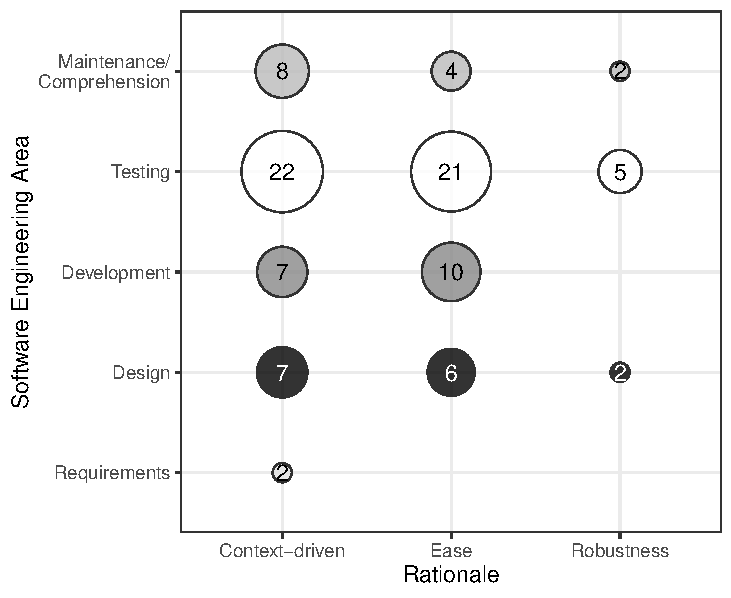
\includegraphics[width=0.8\linewidth]{survey/figures/bubbleplot-rq2.pdf}
%}
\caption{Distribution of rationales per SE area.}\label{fig:bubbleplot-rq2}
    }
\end{figure}

This viewpoint is also evident in papers targeting the detection of cross-browser
incompatibilities (XBIs)~\cite{Choudhary-2010-ICSM, Choudhary-2012-ICST, Semenenko-2013-ICSM,
Choudhary-2013-ICSE, Selay-2014-DICTA, He-2016-ICWS, Xu-2018-TOIT}.
This problem requires developers to detect visual differences between web pages within the same web application when rendered on different browsers.
This task is challenging for a number of reasons. 
First, manually performing this task, for instance through eyeballing, is neither efficient nor easy.
Hence, an automatic technique would require simulating
the reasoning that humans do while \textit{seeing and comparing} two web pages.
This can be easily simulated through a computer vision technique called \textit{image differencing}, for which a plethora of different techniques have been proposed~\cite{Choudhary-2012-ICST,
	Semenenko-2013-ICSM,Choudhary-2013-ICSE}.

However, originally, the same problem was tackled from a non-visual perspective.
First works on XBIs used well-known DOM differencing techniques as a proxy for finding visual defects. %~\cite{}. \andrea{pending cite}
The main limitation was the fact that DOM-level differences do not always
correspond to a different visual layout.
Hence, this caused such techniques to have many false positives and a low accuracy.
On the other hand, visual approaches have been proposed both as an alternative,
as well as, a complementary technique to overcome the limitations of the DOM-based approaches. 

\header{Robustness}
The concept of robustness of a visual approach concerns its capability of maintaining
its effectiveness despite minor visual changes happening in the software being analyzed.

A few papers~\cite{Chang-2010-CHI,Alegroth-2013-ICST,Tanno-2018-ICSTW} mention robustness
as rationale for choosing computer vision.
They explain that visual approaches are used because they are considered more change-tolerant than
alternative code-based techniques. In other words, according to the authors, using a code-based approach for the
same problem is likely to produce a fragile tool that would require a high maintenance cost. 

For instance, \citet{Chang-2010-CHI} describe how spatial re-arrangements of GUI components on the page
can lead to fragile test scripts, a well-known issue in web testing~\cite{Leotta-2016-JSEP}.
According to \citet{Chang-2010-CHI}, visual approaches are more robust to minor layout changes and
elements repositioning.
This viewpoint is discussed and confirmed in the paper by \citet{Alegroth-2013-ICST},
in which image recognition of GUI elements allows the development of more robust system-level automated test suites. 
A similar finding is in the paper by \citet{Stocco-2018-FSE}, in which an image processing pipeline was used to automatically trace web elements across different versions of the same web applications. Their tool \textsc{Vista} exhibited a high test repair rate during software evolution, outperforming a DOM-based test repair solution. This essentially means that in the web domain, web app GUIs exhibit less frequent changes as compared to the DOM, as acknowledged by other researchers~\cite{2015-Leotta-ICST,2016-Leotta-JSEP,Hammoudi-2016-FSE,Hammoudi-2016-ICST}.

The bubble chart of \Cref{fig:bubbleplot-rq2} shows the distribution of the rationales
in relation to the SE areas presented in \Cref{sec:rq1}.
We notice that the context-driven category dominates across all SE areas.
In the areas of requirements, design, and maintenance, visual approaches were
prevalently used because, at this stage of the software development lifecycle,
designers or requirements engineers mostly deal with visual abstractions of
(portions) the software such as GUI mockups, or UML models.
Computer vision allows the transformation of these visual artifacts to support successive SE tasks.
For example, in the work by~\citet{Zhang-2017-ASE}, annotated sketches are used
to specify test requirements and test case creation. In this case, the targeted SE
area is both requirements engineering and testing. 


\header{Summary}
In this section, 
the goal was to understand the rationales and motivations for using computer vision to
address software engineering problems.
An understanding of the rationales can help researchers
decide if their research area or topic has similar problems or challenges,
and then potentially explore using computer vision for their problem.
We identified three types of rationales by collecting and categorizing the reasons stated by the authors of each paper. There are context-driven, ease of use, and robustness.
Papers were classified as context-driven when the context of the software engineering problem itself
has dictated the use of visual approaches.
The ease of use classification was used in cases where the motivation
is not necessarily driven by the context,
but driven by the motivation of making an existing software engineering process easier to use
(e.g. has less manual work, easier to comprehend).
Finally, papers were classified as motivated by robustness whenever the motivation
is making a software engineering task more accurate or less fragile.
Out of all three categories of rationales, the context-driven category was the most common.







% !TEX root =  manuscript.tex
\subsection{Computer Vision Techniques (RQ3)}


In order to investigate how computer vision is applied, we studied:
(1)~what visual artifacts are used, generated, or extracted from the software,
and (2)~what computer vision techniques are used to process or analyze the visual artifacts.
We recall that visual artifacts are visual data (e.g.,  images) used by one or more computer vision
techniques, with the final objectives of addressing a software engineering problem.


\begin{figure}
%    \revised{0.98\linewidth}{
    \centering
    %\fbox{
    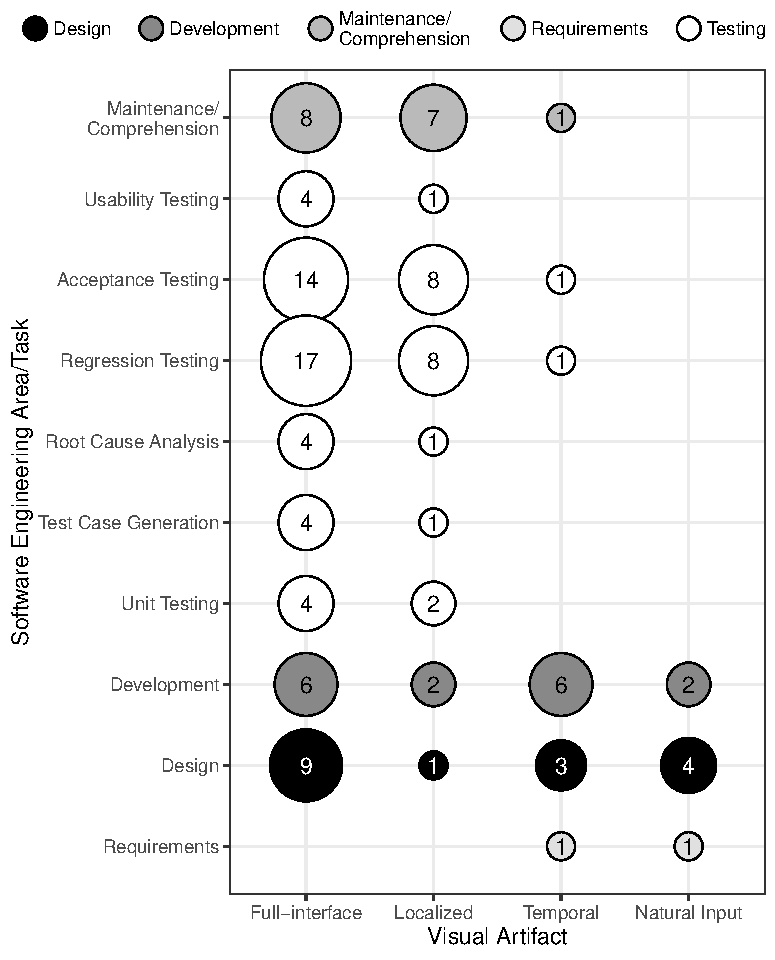
\includegraphics[width=0.8\linewidth]{survey/figures/visual-artifacts-bubble-plot}
    %}
    \caption{Distribution of visual artifacts per SE area \& task.}\label{fig-artifacts}
%    }
\end{figure}



\header{Artifact Categories}
Through our survey of the field, we classified the 
%identified a number of classes of 
visual artifacts used in the literature into four categories:
(1)~full-interface artifacts, (2)~localized artifacts,
(3)~temporal artifacts, and (4)~natural input artifacts. 
\Cref{fig-artifacts} shows the distribution of such visual artifacts 
with respect to the SE area/tasks.

The first category, \emph{full-interface visual artifacts}, typically represents
screenshots of the entire user interface of the system (whether a web browser or
desktop application, as well as other forms such as visual content of TVs and car displays)
~\cite{Choudhary-2010-ICSM,Delamaro-2011-STVR,
Choudhary-2012-ICST,Semenenko-2013-ICSM,Choudhary-2013-ICSE,Nguyen-2015-ASE,
Mahajan-2015-ICST,Deka-2016-UIST, Hori-2015-SEKE,Mahajan-2016-ICST,Feng-2016-ASE,
Patric-2016-ASE,Deka-2017-UIST,Wan-2017-STVR,He-2016-ICWS,Zhang-2017-ASE,Chen-2017-IUI,
Kirac-2018-JSS,Xu-2018-TOIT,Kuchta-2018-EMSE}.
This type of artifact simply has one large screenshot that captures the entire interface. 
This artifact has been used most commonly to capture the \textit{visual state} of the application
(regardless of the platform), and analyzed further to perform various forms of testing
(e.g., regression, acceptance, or test generation).

However, full-interface artifacts capture the visual state of the system at a coarse-grained
level of granularity, which renders them less applicable when a more detailed analysis is needed. This is because the full-interface 
captures the interface as a whole, and is therefore not very useful when the goal is more micro-scale, such as analyzing or recognizing a particular icon for instance. 
For these cases, our survey revealed another category containing  \emph{localized visual artifacts}.
In this case, visual artifacts are created at the level of a 
specific component, an area of interest, or a certain feature \cite{Chang-2010-CHI,
Alegroth-2013-ICST, Mahajan-2014-ASE, Amalfitano-2014-WISE, Selay-2014-DICTA,
Burg-2015-UIST, Leotta-2018-STVR, canvas_icst2018}.
Compared to full-interface visual artifacts, this type of artifact is more beneficial
for scenarios where analysis needs to be performed for a specific component or feature in a system. 
For instance, localized visual artifacts have been used to create a test case for a GUI
(by recording and tracking a single visual artifact for UI elements) \cite{Chang-2010-CHI},
or in debugging the rendering or capturing the behaviour of a specific HTML element in a web application~\cite{Burg-2015-UIST}. 
Had the record-and-playback used full-interface instead of localized visual artifacts, then the analysis wouldn't make much since because the test script operates at the level of elements, not entire interfaces. 

The third category that emerged is \emph{temporal artifacts}, in which the visual information
captures the \emph{dynamic behaviour} of some sequence or chain of information, states, or events
~\cite{Li-2010-CHI, Lin-2014-TSE,Ponzanelli-2016-ICSE,Bao-2017-EMSE}. 
For instance,~\citet{Bao-2017-EMSE} use a temporal artifact (a video screen recording) to construct a
tool to help researchers conducting user studies of developers' behaviours
to automatically distill and transcribe their actions, inputs, and event sequences
by capturing a video screen recording of their work session.

Finally, 
the last identified category is \emph{natural input artifacts}.
These artifacts capture a natural representation or interaction with a human user.
The only example of this artifact that we found in the collected literature are
hand-sketches~\cite{Scharf-2013-ICSE, Reiss-2018-ASEj}.
This type of artifact provides a number of benefits:
(1)~it provides a more intuitive and natural way for software engineers to interact with,
    design, develop, or test their software, and
(2)~it allows a broad degree of freedom in capturing user input,
    which can be useful when modelling or analyzing multi-variable complex systems.



\input{survey/table-algorithms.tex}

\header{Visual Techniques Taxonomy}

\begin{figure}
    \centering
    %\fbox{
    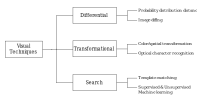
\includegraphics[width=\linewidth]{survey/figures/taxonomy}
    %}
    \caption{Synthesized taxonomy of visual techniques.}
    \label{fig:taxonomy-rq3}
\end{figure}

In this section, we describe a taxonomy of visual techniques.
The taxonomy was synthesized from the pool of papers we collected 
in this survey. 
This taxonomy has not been used elsewhere, since 
there are no existing surveys on the use of computer 
vision techniques in software engineering.
For each paper, we analyzed the text and 
noted down the computer vision algorithms utilized by the authors 
to solve the software engineering problem being tackled.
After conducting this process over all collected papers, 
we grouped the algorithms and identified three main patterns of algorithms,
which are then collected in a taxonomy.
We built the taxonomy in an iterative manner,
where a new taxonomy category is defined if a certain computer vision algorithm 
can not be classified under any of the existing categories.

\autoref{fig:taxonomy-rq3} shows the resulting taxonomy.
As shown in the figure, we identified three main categories
of visual techniques used in software engineering research:
(1)~differential, (2)~transformational, and (3)~search techniques.
Each technique has sub-categories of algorithms, which will be described in Section \ref{sec:CV-algos}.


\emph{Differential techniques}: a visual analysis process that takes  two or more visual artifacts as input, and outputs their differences~\cite{Delamaro-2011-STVR,Choudhary-2012-ICST,
Choudhary-2010-ICSM,Alegroth-2013-ICST,Choudhary-2013-ICSE,Lin-2014-TSE,Mahajan-2014-ASE,
Amalfitano-2014-WISE,Selay-2014-DICTA,Burg-2015-UIST,Mahajan-2015-ICST,Hori-2015-SEKE,
Mahajan-2016-ICST,Feng-2016-ASE,Deka-2017-UIST,He-2016-ICWS,Kirac-2018-JSS,Xu-2018-TOIT}. 
The nature of these differences is typically case-specific and often targets a specific
feature that the paper is considering.
Differential techniques are commonly used in situations where a comparison of different aspects,
options, or versions of the software is desired.
For instance, they have been widely utilized for cross-browser testing
~\cite{Xu-2018-TOIT, Choudhary-2010-ICSM, He-2016-ICWS, Choudhary-2012-ICST, Selay-2014-DICTA},
where the goal is to check for any differences between two or more browsers in the way they 
render a web app.

The second category, \emph{transformational techniques}, achieve a specific software engineering task
by transforming the visual artifact into a more abstract type of information
~\cite{Scharf-2013-ICSE,Semenenko-2013-ICSM,Nguyen-2015-ASE,Deka-2016-UIST,Ponzanelli-2016-ICSE,
Patric-2016-ASE,Wan-2017-STVR,Bao-2017-EMSE,Zhang-2017-ASE,Reiss-2018-ASEj,canvas_icst2018,Kuchta-2018-EMSE}.
This transformation is typically case-specific, as the higher-level abstract information
is used to solve the specific instance of problems addressed in the paper.
For instance, this approach has been used to allow manual hand-drawn strokes as a method to specify
test executions and requirements~\cite{Scharf-2013-ICSE},
where transformational techniques are applied on hand-drawn stroke instances to extract testing
instructions and assertions from the strokes, and finally generate a working test case.

Finally, the third category is \emph{search techniques}~\cite{Chang-2010-CHI, Li-2010-CHI,Chen-2017-IUI,Leotta-2018-STVR}.
In this case, a visual artifact is used as a key to find information within a larger set of visual artifacts.
A popular example of this approach is visual record-and-playback tools such as Sikuli~\cite{Chang-2010-CHI}.
These tools first record component visual artifacts for every GUI element clicked or interacted with
by a developer or user, and then, in the playback phase, a visual search method is employed to locate
the element on screen to perform the recorded action (e.g., click).

\begin{figure}
%    \revised{\linewidth}{
    \centering
    %\fbox{
    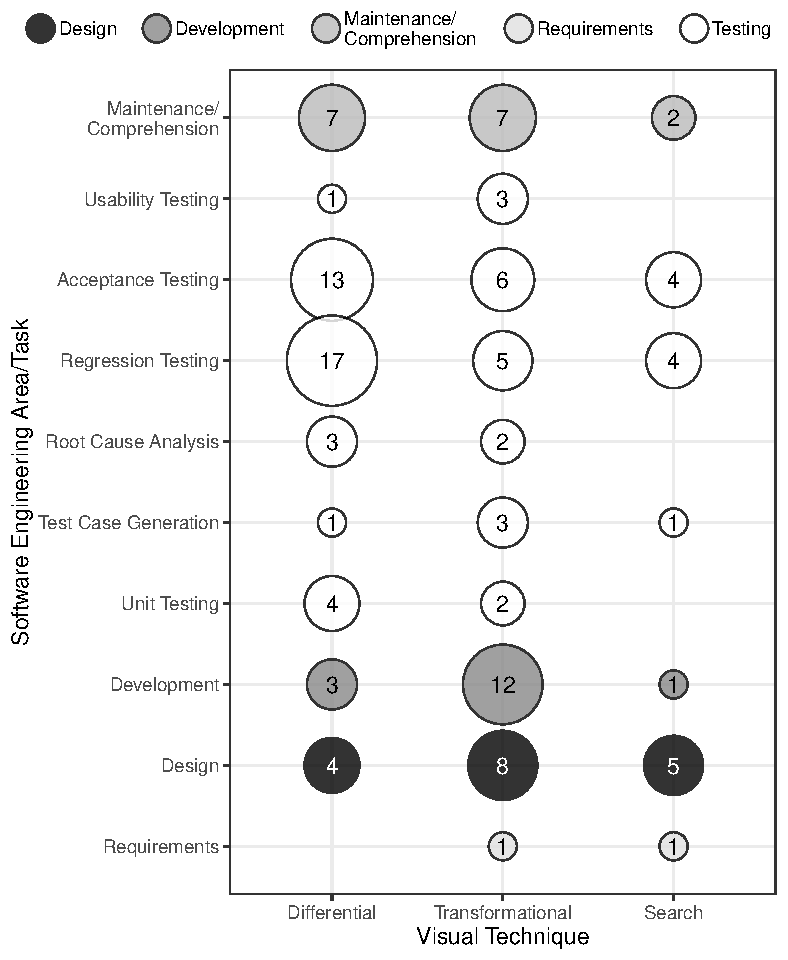
\includegraphics[width=0.8\linewidth]{survey/figures/bubbleplot-rq3}
    %}
    \caption{Distribution of visual techniques per SE area \& task.}\label{fig:bubbleplot-rq3}
%    }
\end{figure}


In order to have a better insight on the use of different 
categories of visual techniques,
the bubble plot of \autoref{fig:bubbleplot-rq3} shows their distribution over the various SE areas.
In the plot, software testing has a finer-grained granularity
since it is by far the most represented area in our final pool of papers.
We make a number of observations from the plot.
First, we notice that transformational techniques are more uniformly represented across all SE areas and tasks.
This is a somewhat expected result 
since transformational techniques are generic enough to be used 
on their own, or in addition to other techniques as pre- or post-processing steps. 
Next, we also notice that differential techniques were relatively common in testing tasks.
For instance, regression and acceptance testing greatly benefit from differential techniques,
since they are very well aligned towards detecting differences and therefore suitable for indicating regression faults.

    
\subsubsection{Computer Vision Algorithms}
\label{sec:CV-algos}

In addition to the preceding analysis of the high-level categories of visual techniques,
we also examine the specific computer vision algorithms used in the collected pool of papers.
\autoref{tbl:cv-algorithms} shows the algorithms that have emerged from our analysis.
We now describe each of the identified algorithms.

\header{Image Diff}
In these CV algorithms,
a pair of images is taken as input
and the output is defined as a function of the \emph{difference}  between the pair.
Various instances of these algorithms differ in their choice of the output function.
For instance, the most common variation uses the raw absolute difference as the output value~\cite{Choudhary-2010-ICSM,Li-2010-CHI,Mahajan-2014-ASE,Ponzanelli-2016-ICSE,
Deka-2017-UIST,Bao-2017-EMSE,Chen-2017-IUI,Kirac-2018-JSS,Moran-ICSE-2018},
where it is useful for faithfully detecting any \textit{pixel-level} difference.
Another variation adopts a more relaxed approach
where the output function captures only \emph{perceivable} differences by humans
using algorithms such as PID (Perceptual Image Differencing)~\cite{ref:PID},
PHash (Perceptual Hashing)~\cite{ref:PHash},
and Structural Similarity Index (SSIM)~\cite{ref:SSIM},
which aim to reduce false positives by mimicking human perception.
These techniques were utilized in~\cite{Mahajan-2015-ICST,Mahajan-2016-ICST,
Xu-2018-TOIT,Moran-ICSE-2018,Moran-2018-ASE,Burg-2015-UIST}. 

\header{Probability Distribution Distance}
These algorithms quantify distances in \emph{populations} of pixels,
as opposed to a pixel-wise comparison.
The goal here is to measure how similar two given distributions are,
such as image \emph{histograms}~\cite{223129} which give the distribution of pixels in an image.
This is then used to establish whether the two
distributions of pixels can be assumed to represent similar visual
information.
The $\chi^2$ histogram distance (for both coloured and grayscale data)
is by far the most commonly used distribution distance
in our pool of papers~\cite{Choudhary-2012-ICST,Choudhary-2013-ICSE,
Hori-2015-SEKE,Feng-2016-ASE,He-2016-ICWS, Moran-2018-ASE},
as it is readily available in many implementations
and provides a simple and effective approach for the needed quantification of distance.

\header{Color/Spatial Transformation}
These algorithms perform a transformation
of the spatial or color-space of one or more images~\cite{Li-2010-CHI,Patric-2016-ASE,Wan-2017-STVR,Kirac-2018-JSS,
canvas_icst2018,Moran-TSE-2018,Moran-ICSE-2018,Xiao-2019-ICSE}.
This constitutes applying a 2D or 3D transformation matrix
on the desired geometric space (e.g., a rearrangement of color-space).
This class of algorithms has been used in our pool of papers
to perform tasks such as extracting structure from images,
aligning images, and various forms of thresholding to extract content.

\header{Optical Character Recognition (OCR)}
OCR algorithms use a series of computer vision analyses
to recognize strings in images.
Once the string is recognized, another sequence of steps
converts each character in the image to textual data.
We found multiple papers in our pool (e.g., \cite{Chang-2010-CHI, Amalfitano-2014-WISE,
Nguyen-2015-ASE, Ponzanelli-2016-ICSE, Bao-2018-TSE, Tanno-2018-ICSTW, Xiao-2019-ICSE})
which have used OCR for tasks such as checking GUI component labels and
generating component labels from mockups/screenshots.

\header{Template Matching}
Another major class of CV algorithms used in the papers is template matching.
Here, one image is searched within another image or set of images.
That is, a visual scan is performed to find a template image (hence the name)
in a larger image or set of images.
Several papers in our pool~\cite{Chang-2010-CHI, Semenenko-2013-ICSM,
	Lin-2014-TSE, Bao-2017-EMSE, Chen-2017-IUI, Leotta-2018-STVR,
	Stocco-2018-FSE, Tanno-2018-ICSTW} have used this approach
to achieve tasks such as locating and finding coordinates of components and
checking the presence/absence of components or certain features within
a set of GUIs. While it may appear that template matching 
is related to the OCR class of techniques, it is actually different. 
This is because OCR converts an image to a string, while template matching finds the location of a given image within another image. 

\header{Machine Learning}
Machine learning has also been used by a few papers in our pool.
For instance, \emph{decision trees} were used for classifying web pages
in cross-browser testing~\cite{Choudhary-2012-ICST,Semenenko-2013-ICSM}.
\emph{Convolutional neural networks} (CNNs) were also used
to analyze GUIs and their content~\cite{Moran-TSE-2018,Semenenko-2013-ICSM}.
Furthermore, scale- and transformation-invariant features
(e.g.,  SURF--Speeded-Up Robust Features~\cite{ref:SURF}, Wavelets~\cite{ref:wavelet}),
which are basically features aiming at analyzing image structure and content,
were used to classify and detect GUI elements
~\cite{Xiao-2019-ICSE,Stocco-2018-FSE,Kuchta-2018-EMSE,Bao-2017-EMSE}.


\input{survey/table-cvlibs}


\header{Libraries and Tools}

% \revised{0.48\textwidth}{
\changed{
We also investigated what industrial or open-source 
libraries and tools were used by the papers in their 
implementation of computer vision techniques. 
\autoref{table:cvlibs} shows a list of the CV tools 
or libraries that have been used by the papers in our pool. 
The first column reports the name of the tool or library. 
The second column describes the scope of the library, 
and the last column shows the paper(s) that utilize 
a certain library to implement their CV analysis or processing. 
Papers that do not state which library or tool they used are not 
included in the table, and therefore the number of papers 
in the table is smaller than the total pool.
For the sake of completeness, we also included other 
CV tools and libraries that have not been used by 
any of the papers in our pool, which are marked 
by the ``N/A'' (not applicable) value in the last column. 
These tools were included in order to present the software 
engineering research community with an easy access to a list of 
other computer vision tools that they might find helpful to use. 
Due to the absence of queryable databases in 
which computer vision tools are listed, we resorted 
to manual search engine queries to find computer 
vision tools or libraries other than those already 
used by our pool. The queries we used were of the 
form ``alternative (libraries or tools) to X'', 
where X is one of the libraries already in our pool. %\andrea{vague}

The most commonly used library is \emph{OpenCV}.
\footnote{https://opencv.org} This library has 
implementations for a large number of CV algorithms, 
including all the algorithms we report in this 
survey (Section \ref{sec:CV-algos}). It was first 
released in 2000, and is still in active development. 
Other than OpenCV, a few other libraries were used 
by only a handful of papers. 
\emph{ImageMagick}\footnote{https://imagemagick.org/} 
is a simple and easy to use library offering basic 
quick image manipulations (e.g.,  resize, rotate).  
\emph{ImageJ}\footnote{https://imagej.net} is also 
quite similar in features and scope.
\emph{Tesseract}\footnote{https://github.com/tesseract-ocr/tesseract} 
is a popular open-source library that is modular and extensible, 
with support for more than 100 languages.
\emph{Abby FineReader}\footnote{https://abbyy.com/} is 
a commercial library that focuses specifically on 
OCR and includes many related preprocessing/postprocessing 
algorithms, as well as various file formats.
\emph{BoofCV}\footnote{http://boofcv.org} focuses 
on performance-tuned algorithms and is geared 
towards cases where real-time response is priority.
\emph{ITK}\footnote{https://itk.org/} focuses on 
high-dimensional visual data often present 
statistics and science, and also has extensive 
image coordinates matching algorithms that 
might be beneficial in a number of image 
matching applications. 
\emph{VLFeat}\footnote{https://vlfeat.org/} is 
geared towards implementing a wide variety of 
feature extraction and matching algorithms, 
enabling applications in image search or transformation.
Finally, there are cloud-based tools offered by 
major cloud hosting providers (e.g. Amazon Web 
Services, Google Cloud Platform, Microsoft Azure). 
The defining feature of these services is their 
cloud nature and the availability of many 
pre-trained computer vision models for various 
visual tasks, such as content tagging and 
visual path analysis. 
}

\begin{table}[]		\scriptsize
	\caption{Summary of the analysis approaches for the targeted research problems.}
	\begin{tabular}{lll}
		
		\textbf{Non-functional Property} & \textbf{Research Problems}                                                                        & \textbf{Approach}                                                                                                                                                                                                                                         \\
		\hline \\
		
		Accessibility           & \begin{tabular}[c]{@{}l@{}}- testing semantic roles\\ - repairing form labels\end{tabular} & \begin{tabular}[c]{p{4.5cm}}
			- identifying page regions, then computing and sorting ratios of visual locations, areas, visual size variance, and neural network classification. 
			\\ - abstracting form elements, then combining visual layout (relative spacing) with visual prominence (weight, size, color), and finally  optimizing label assignment
		\end{tabular} \\
		%		\begin{tabular}[c]{p{4.5cm}}Existing works perform syntax checks. Semantic roles and form labels are not tested or repaired. The work in this dissertation tests roles and repairs labels by analyzing visual cues from the page.\end{tabular} \\
		
		\\
		\hline \\
		
		Maintainability         & \begin{tabular}[c]{@{}l@{}}- generating reusable \\ components\end{tabular}                & 
		\begin{tabular}[c]{p{4.5cm}}- visual normalization of the page based on 
			element location, dimensions, and type, followed by histogram clustering \end{tabular} \\
		
		
		\\
		\hline \\
		
		Testability             & - testing canvas elements                                                                  & \begin{tabular}[c]{p{4.5cm}}- detecting and isolating object boundaries, then identifying their shapes, dimensions, colors, and hierarchy \end{tabular}                              \\
		
		
	\end{tabular}
	\label{tbl:summary-techniques}
\end{table}

\header{Overview of the proposed techniques}
In this dissertation, we propose a number of visual analysis techniques 
to improve the non-functional properties of testability, accessibility, and 
maintainability. An introduction to these properties and the motivation for 
exploring them is discussed in \Cref{chp:intro}. In \Cref{tbl:summary-techniques}, 
we show an overview of the approaches used, which are presented here only in a high-level and will be discussed in detail in their relevant chapters. 
While existing works are mostly based on using entire images, say, for diffing or searching, the techniques in this dissertation operate at a fine-grained level of analysis. By fine-grained we mean that the analysis focuses on very specific visual features that may potentially be helpful in addressing the research problem. 
For instance, when we analyze canvas elements, 
one fine-grained aspect that is used is extracting and identifying the boundaries 
of each object, in order to help detect the type of each object and express it in the 
DOM. Accordingly, the approaches are based on identifying what fine-grained features should be selected, where should they be collected from, how would they be combined,  
and how to analyze them to address the research problem. Each of these aspects 
is problem specific and need to be explored and determined according to the objective and constraints of the problem. 

\header{Summary}
The goal of this subsection was to explore what computer vision techniques
were used and what visual artifacts were extracted from the software.
To this end, we identified four categories of artifacts.
The first category, full-interface artifacts, represents cases
where the entire visual content of a software is used (e.g.,  entire desktop interface, entire console).
The second category is localized artifacts, where only a specific module
or component of the software is captured visually. 
Third, temporal artifacts capture the dynamic behavior of the states or events in a software. Finally, natural input artifacts capture natural forms of input by humans (e.g.,  hand sketches).
%
Visual artifacts are then processed by one or more of three visual techniques.
The first category, differential techniques, are based on various forms of contrasting two or more visual artifacts and using the differences to solve a software engineering problem.
The second category, transformational techniques, rely on transforming the visual artifact into a more abstract data structure on which further analysis can be conducted.
Finally, in search techniques, a visual artifact is used as a key to find information within a larger set of visual artifacts.

\autoref{tbl:cv-algorithms} shows the major computer vision algorithms used in the collected papers.
The visual technique column describes the high-level goal of what the algorithm is trying to achieve visually.
The algorithm column lists the specific algorithms that were used to achieve the task.
For instance, when papers wanted to do a differential examination of visual artifacts, the two computer vision approaches that were used were image diffing and distribution distances.



% !TEX root =  manuscript.tex
\subsection{Evaluation and Challenges (RQ4)}


\header{Evaluation Methods}

We systematically studied the selected papers to 
understand the most common methods used for 
evaluating the proposed visual approaches.
\Cref{table:evaluation-techniques} (Evaluation 
Methods) depicts the results: the evaluation 
methods presented are not necessarily disjoint,
since one technique can for instance be evaluated 
with respect to its performance (i.e., running time), 
and its accuracy calculated by the judgment of human participants.

In more than half of the works (53\%), the 
evaluation methods were performed using 
wide-spread effectiveness assessment 
measures such as precision and recall
~\cite{Choudhary-2010-ICSM, Choudhary-2012-ICST, 
Choudhary-2013-ICSE, Lin-2014-TSE, Nguyen-2015-ASE, 
Mahajan-2015-ICST, Hori-2015-SEKE, Feng-2016-ASE, 
Patric-2016-ASE, Wan-2017-STVR, He-2016-ICWS, 
Bao-2017-EMSE, Chen-2017-IUI, Reiss-2018-ASEj, 
Kirac-2018-JSS, canvas_icst2018, Kuchta-2018-EMSE, 
Xu-2018-TOIT}.

Another significant body of work measured 
the manual effort saved by the visual approach 
with respect to the humanly performed 
task~\cite{Delamaro-2011-STVR, Li-2010-CHI, 
Li-2010-CHI, Semenenko-2013-ICSM, Mahajan-2015-ICST, 
Feng-2016-ASE, Chen-2017-IUI, Leotta-2018-STVR, 
Reiss-2018-ASEj}. 
Moreover, several works also evaluated the 
performance of the proposed approaches, 
usually measuring the running time on common 
developer platforms (i.e., mid-level 
notebooks)~\cite{Nguyen-2015-ASE, Selay-2014-DICTA, 
Hori-2015-SEKE, Patric-2016-ASE, Wan-2017-STVR, 
Bao-2017-EMSE, Reiss-2018-ASEj, Kirac-2018-JSS}.

Performance is potentially considered as 
important as the accuracy because image analysis 
techniques are deemed as being computationally 
expensive. Thus, their application and use must 
carefully evaluate the overhead imposed by 
these visual approaches over the most general 
SE tool being developed. Initially, this might 
not favor their adoption if compared to other 
less computationally-intensive approaches.
However, the authors report that the time 
taken by their proposed techniques are all 
reasonable in common processing environments, 
suggesting that execution time should not be 
considered as a deterrent decision criterion when 
adopting a visual approach to support a SE task.

In several works, the human expertise was used to 
assess the output of the visual 
techniques~\cite{Mahajan-2015-ICST, Hori-2015-SEKE, 
Mahajan-2016-ICST, Kuchta-2018-EMSE, Xu-2018-TOIT, 
Ponzanelli-2016-ICSE, Choudhary-2010-ICSM, 
Choudhary-2012-ICST, Choudhary-2013-ICSE}.
As an example, \citet{Mahajan-2015-ICST} examine 
the efficacy of WebSee (a tool that identifies 
presentational failures in HTML pages)
through manual investigation of its output
when it is executed on 253 automatically-generated 
test cases.
This is done to see whether WebSee is able to 
correctly identify the faulty HTML elements
seeded when generating the test cases.
While we were expecting more human judgment 
involved in the evaluation of the selected papers, 
its application depends largely on the context 
and the problem being solved. 

Four works do not propose a quantitative empirical 
evaluation of the proposed technique, but 
rather present them by means of use cases.
A closer look at these publications revealed 
that two of them are short papers~\cite{Alegroth-2013-ICST, Scharf-2013-ICSE},
where having a more thorough evaluation is not 
mandatory. 
The other two papers~\cite{Burg-2015-UIST, 
Deka-2016-UIST} were published at the ACM Symposium 
on User Interface Software and Technology (UIST), 
in which use case demonstrations appear to be more frequent.
Four works included an industrial 
evaluation~\cite{Li-2010-CHI, Mahajan-2015-ICST, 
Amalfitano-2014-WISE, Kuchta-2018-EMSE} where the work is evaluated 
through feedback or measurements in an industrial setting.

\input{survey/rq4-table}


Finally, 
we noticed diversity in the evaluation methods of techniques aimed at solving similar problems. 
For example, several works have been proposed to identify some sort of \textit{visual defects} (e.g., all the approaches dealing with XBI). 
Four of these techniques~\cite{Mahajan-2014-ASE, Mahajan-2015-ICST, Mahajan-2016-ICST, Patric-2016-ASE} use ``seeded faults'' as an approach for constructing test oracles, whereas others take a different evaluation path. 
For instance, \citet{Choudhary-2013-ICSE} manually count all XBIs detected by different tools (i.e., their agreement)
as an upper bound for the number of issues that an XBI detection tool should identify, and use this number to compute the recall of X-PERT. As a further evaluation, authors could have been also evaluating their technique using seeded XBIs
to broaden the evaluation. 
Conversely, the works that only use seeded faults could use the agreement of multiple fault detectors to compute recall. 
This scenario essentially suggests that the evaluation of some of the proposed techniques in the literature can be substantially improved by leveraging the evaluation approaches from other techniques that aim at solving similar problems. 

\header{Challenges and Limitations}

Evaluations also exposed the main challenges and limitations that authors faced while developing their visual-based solutions. 
Unfortunately, a subset of the papers (41\%) either do not explicitly discuss drawbacks for the visual approach being evaluated, or do not provide concrete failing examples. On the other hand, the majority of the papers (59\%) do report the challenges encountered during the experimentations, summarized in \Cref{table:evaluation-techniques} (Challenges),  which we describe next. 

\header{Noise} 
The most recurring technical issue that inhibited the correct functioning of visual approaches concerns the \textit{noise} present in the visual artifacts~\cite{Ponzanelli-2016-ICSE,Reiss-2018-ASEj,Bao-2017-EMSE,Nguyen-2015-ASE,Kuchta-2018-EMSE,Leotta-2018-STVR,Li-2010-CHI,Lin-2014-TSE}. 
Noise refers to the presence of other random or overlapping items in the background of the visual artifact that prevents, for instance, the correct detection of the target object. Hence, before applying the desired visual method, a pre-processing technique is often used to clear the noise out of the artifact. 

As an example,~\citet{Ponzanelli-2016-ICSE} apply OCR to detect source code in frames sampled from video tutorials. However, the effectiveness of OCR fluctuates dramatically if the considered frame's background contains non-pertinent information. As a solution, the authors utilize two additional visual techniques---shape detection and frame segmentation---in order to focus OCR towards the area of interest.

Another more specific noise-related limitation pertains to the \textit{sensitivity} of the visual approach to theme/surroundings changes, lighting conditions, and reflections~\cite{Chang-2010-CHI,Kirac-2018-JSS,Leotta-2018-STVR,Kuchta-2018-EMSE,Li-2010-CHI,Lin-2014-TSE}. A possible mitigation concerns using threshold parameters to limit their detrimental effect. 

\header{Dynamicity} Highly-variable visual artifacts are also a major challenge for the design and development of reliable visual approaches. 

One source of fragility is due to animations~\cite{canvas_icst2018,Chang-2010-CHI,Choudhary-2010-ICSM}. Indeed, a continuously-changing visual artifact (e.g., a video frame) represents a major limitation for many one-shot techniques. As a possible solution, such techniques would need to be applied repeatedly, similarly as real-time domains, or, in extreme cases, re-designed from scratch to meet the new domain requirements. 

Another source of fragility is due to web advertisements~\cite{Wan-2017-STVR}.
An ad is rendered as a dynamic component within a more static container (i.e., a web page),
the visual representation of which usually changes across consecutive loads of the web page or over different time stamps.
Visual methods need to isolate the dynamics of web pages to avoid erroneous behaviour or false positives.  

\header{Recognition}
Another challenge of visual approaches that emerged from our study concerns (1)~accurately identifying small imperceptible differences between images and (2)~recognizing complex user-defined actions such as manually inserted strokes or handwriting. 

For example, a source of false positives in \textsc{VISOR}~\cite{Kirac-2018-JSS}, an image comparison technique used for black-box testing of digital TVs, is the tiny differences that occur when rendering accent characters on the screen (e.g., cedillas). 
Typically, the choice on whether such differences should be considered as defects or not is left to human's perception. 
%
Two other works experienced recognition issues, but not at the same pixel-level as \textsc{VISOR}. \citet{Bao-2017-EMSE} discuss problems in detecting visual fine-grained developers' actions from videos, such as code editing, text selection, and window scrolling. Similarly,~\citet{Scharf-2013-ICSE} mention issues in detecting handwriting in manually-produced sketches. 

These findings demonstrate how complex is the set of visual differences that can emerge while comparing two images, and how vast and multifaceted is the set of input actions that are possible on a user interface. Indeed, when a visual method is used to actively support the \emph{end user}, they arguably need to recognize a broader set of inputs than those they would receive from another algorithm, if they were executed in a software controlled environment. This poses new challenges to the development of robust visual approaches for aiding SE.


\header{Visibility}
At last, in four works, having the visual artifact present in the main rendering area is mentioned as a requirement for the visual technique to effectively fulfill its task.
This requirement can be violated by, e.g., \textit{fading}~\cite{Chang-2010-CHI,Leotta-2018-STVR} and \textit{scrolling}~\cite{Choudhary-2010-ICSM,Bao-2017-EMSE}.

As an example, \citet{Leotta-2018-STVR}'s tool \textsc{PESTO} uses template matching to detect the optimal visual locator corresponding to a web element on the page. However, the web element of interest might be outside the actual rendered web page. This happens when a long and complex form with multiple fields cannot be entirely visualized within the main screen. The authors propose an engineering workaround to solve issues related to scrolling: if the visual artifact being searched is not immediately displayed, the tool scrolls the page down automatically and the template matching is repeated.




% !TEX root =  manuscript.tex
\section{Discussion}\label{sec:discussion}

\header{Increasing Adoption of Visual Approaches}
Our findings show a general growth trend in the adoption and use of visual approaches
in the SE community.
Most of the surveyed papers explicitly recognize, and empirically
demonstrate, the contribution brought by visual methods in supporting SE tasks.

Based on our examination of the literature,
we attribute this increase to two factors.
First, many software developed nowadays have a GUI or other visual interfaces.
The end-user experience is increasingly becoming more important in adding value
to software, and therefore the adoption of visual methods is expected to
increase further in the next years.
Our examination of the trend of number of annual publications 
already shows this trend of increasing number of works utilizing 
visual techniques.
Second, the rapid pace of improvement in hardware and processor architecture has made
the efficiency and run time of advanced visual techniques feasible in common
development environments, which we expect will cause an increased adoption of
visual approaches further down the line.

\header{Software Testing a Major Driver of Visual Approaches}
The majority of papers (around 75\%) have focused on the research area of
software testing.
Our intuition behind this is two-fold.
First, testing is one of the most active SE research areas in general,
so it is not surprising that most of the collected papers fall
within this category.
Second, testing is largely a tooling-based research area, in which
tool prototypes are developed and empirically evaluated.
Many different static and dynamic analysis tools are proposed each year
to facilitate test engineers' activities. 
The results of this survey show that the visual perspective of the software
has been recently used to complement static and dynamic analysis because
it provides a novel and complimentary perspective of the software under test.
The types of analyses that are performed on the presentation-level of the
application would be likely very difficult to perform by analyzing the source code only,
especially with the increasingly complex interfaces and the great emphasis
placed on user experience, of which the interface is a cornerstone component.


\header{Custom Solutions}
The visual techniques used in the collected papers are often ad-hoc solutions developed for tackling a specific problem. 
Authors recognize that it is unlikely to have a consolidated and broadly-accepted solution.  
More specifically, all collected papers have discussed, to some extent, the need of visual approaches for parameter fine-tuning, such as optimal threshold selections. 
In contrast, as will be discussed in the next chapters, the 
techniques proposed in this dissertation aim to minimize or eliminate the need for parameters or thresholds whenever possible. 

Manipulating visual artifacts through a visual technique is highly application-specific, both in the adopted approach and in the considered domain~\cite{2020-Yandrapally-ICSE}. 
For instance, this survey highlights a large body of work in the area of
cross-browser incompatibility.
The authors of these papers have adopted a large variety of solutions
(or incremental variations) to tackle the same problem.
To mention a few,~\citet{Choudhary-2010-ICSM} use an image comparison measure
based on Earth Mover's Distance (EMD), whereas ~\citet{Mahajan-2015-ICST} adopt
perceptual differencing, and~\citet{He-2016-ICWS} compare the colour histograms,
among other approaches.
This trend can be partially explained by the need of proposing and experimenting
with novel and potentially useful techniques.
However, a researcher approaching this topic for the first time could be
somewhat disoriented.
In fact, given that the solutions for the same problem are many,
and they are often evaluated on different benchmarks,
it is not straightforward to find an agreement on what the best technique could be. 
This led to a landscape where each work would typically experiment with a custom
visual processing pipeline to address the specifics of the SE task at hand.

\header{Need for Visual Benchmarks in SE}
We highlight the lack of comparative visual benchmarks on which to evaluate
the plethora of visual approaches utilized in software engineering research. 
A repository of standard, well-organized, categorized, and labeled visual artifacts could
be very useful to support empirical experiments, and to guide
the next generation of research utilizing visual approaches
for software engineering tasks.
Such repositories exist in traditional
(non-visual) software engineering research,
such as SIR~\cite{Do:2005:SCE:1089922.1089928},
Defects4J~\cite{Just:2014:DDE:2610384.2628055}, SF100~\cite{sf100}, and BugsJS~\cite{bugsjs:icst19,2020-Gyimesi-STVR}. This has not been the case, however, for visual techniques in software engineering.
For instance, having analogous repositories for visual bugs can foster
further applications of visual methods in software testing. 
In the issues discussed in this dissertation, which are all non-functional properties, no visual benchmarks exist either, since 
the field is still at its early stages and hasn't matured yet to the degree of creating benchmarks. 

Similarly, object detection and classification tasks need labeled images.
In computer vision literature, there exist some pre-validated and labeled visual
benchmarks, such as ImageNet~\cite{Russakovsky:2015:ILS:2846547.2846559},
BSDS500~\cite{MartinFTM01}, or Caltech 101~\cite{Fei-Fei:2006:OLO:1115692.1115783}.
In software engineering,
a benchmark of labeled visual artifacts might
aid in developing visual techniques,
or training systems for machine learning and deep learning
scenarios.
A notable step in this direction has been carried out 
in the Rico~\cite{Deka-2017-UIST} repository. 
The repository contains around 70k labeled UI screenshots, 
each of which are labeled with 
visual, textual, structural, and interaction trace data.
The dataset facilitates software engineering tasks 
related to the UI, such as UI design search, UI layout generation, 
and UI code generation.


\header{Maintainability of Visual Artifacts}
The visual artifacts created or extracted from the software 
are rarely static across time,
especially for rapidly evolving software such as in agile environments.
The artifacts would therefore have to be frequently modified
or updated to keep track of the underlying evolving software.
\citet{Alegroth-2013-ICST} indicate that
the maintainability of visual artifacts
produced and used by the visual testing tools
as being a major challenge of the
visual-based testing approaches.
Potential research directions to mitigate this challenge 
include proposing strategies for conducting cost-benefit analysis
depending on the expected degree of visual evolution of the software,
and devising automated techniques to
help with or reduce the maintainability
effort for visual artifacts. 


\header{Familiarity with Computer Vision}
Perhaps the biggest challenge hindering a wider adoption
of visual approaches in software engineering
is the lack of familiarity with computer vision techniques.
For instance,
\citet{Delamaro-2011-STVR} describe how developers
should have basic knowledge of image processing
in order to even \textit{use} the proposed tool in the paper.
This is because the visual artifacts can structurally vary with each use,
and thus sometimes one or more manual image processing adjustments
need to be performed before being able to process the visual artifacts. 
In the work proposed in this dissertation, we mitigate this issue 
by proposing techniques that reduce or eliminate the need for parameters or adjustment thresholds, in order to improve robustness. 

\header{Threats to Validity}
The threats to validity of this survey are the bias in the papers' selection and misclassification of the pool of papers in the various research questions. We mitigate these threats as follows.
Our paper selection was driven by the keywords related to visual approaches and software engineering (see Section~\ref{sec:collection}). 
We may have missed studies that use visual methods in the software engineering activities that are not captured by our terms list.
To mitigate this threat, we performed an issue-by-issue manual search of the major software engineering conferences and journals, and followed through with a snowballing process.
Concerning the papers' classification, we manually classified all selected papers into different categories based on the targeted SE area, as well as, more fine-grained sub-categories based on their domains, tasks, and the utilized visual methods (see Section~\ref{sec:results}). 
\changed{Identifying the rationale from the papers that do not explicitly mentioned it  involved some subjectivity and may have resulted in suboptimal mappings, which constitutes another threat.} However, there is no ground-truth labeling for such classification. To minimize classification errors, the first three authors of this chapter have carefully analyzed the full text and performed the classifications individually. Any disagreements were resolved by further discussion.

% !TEX root =  manuscript.tex
\section{Conclusions}\label{sec:conclusions}
A recent and growing trend in software engineering 
research is to adopt a \emph{visual perspective} of 
the software, which entails extracting and processing 
\textit{visual artifacts} relevant to the software being analyzed. 
To gain a better understanding of this trend,
in this chapter, we surveyed the literature on the use of 
visual analysis approaches in software engineering. 
From more than \initialPoolSize publications, 
we systematically obtained \numberOfPapers papers 
and analyzed them according to a number of research dimensions.
Our study revealed that visual analysis techniques 
have been utilized in all areas of software engineering, 
albeit more prevalently in the software testing field.
We also discussed why visual analysis was utilized, 
how these techniques are evaluated, and what limitations they bear.
Our suggestions for future work include the development 
of common frameworks and visual benchmarks to collect 
and evaluate the state-of-the-art techniques, 
to avoid relying on ad-hoc solutions. We believe that 
the findings of this work illustrate the potential of 
visual approaches in software engineering, and may help 
newcomers to the field in better understanding the research landscape.

\hl{A number of key findings can be observed from the survey in order to help in 
guiding and framing the remainder of the dissertation. 
First, cross-browser testing is by far the most common area of application, 
whereas exploring non-functional properties received little to no focus. 
This shows that there is an opportunity to explore the use of visual analysis 
in improving non-functional properties, and therefore the remainder of the dissertation 
will be focusing on this aspect. This will provide better and more novel research 
contributions compared to exploring functional properties. 
Furthermore, our survey of the visual analysis techniques used shows that the 
majority of existing works use some form of basic image diffing or features. This shows that it would be novel and potentially useful to investigate more fine-grained level of visual analysis that examines fine-grained visual details. Accordingly, this unexplored approach will be the basis of the techniques proposed in the remainder of the dissertation.}  


\balance


%\bibliographystyle{IEEEtranN}
%\bibliography{bibliography-short}

\chapter{Web canvas testing}
\label{chp:testability}

\section{Introduction}\label{sec:introduction}
Canvas elements are one of the major web technologies used to deliver interactive and dynamic graphics-intensive web applications. Canvas-based web applications are utilized in a wide variety of fields, such as math and science education~\cite{arreola2017creating}, geographical modelling~\cite{christen2012web}, and genetics research~\cite{buels2016jbrowse}. 
The \texttt{<canvas>} element on the HTML page is only a container for graphics, which is updated programmatically, via its APIs, through JavaScript code.

From a testing perspective, however, there has been little to no progress in the literature in terms of testing canvas elements. None of the works surveyed in Chapter 2 perform canvas testing. In addition, existing web testing methodologies do not apply to canvas elements for the following reasons. The testing of web applications in practice is based on using a browser automation tool, such as Selenium\footnote{http://www.seleniumhq.org/} or PhantomJS\footnote{http://www.phantomjs.org/}, to make assertions on the DOM (Document Object Model) of the webpage, which is a tree representation of the current set of nodes in a page. This approach opens the web application and analyzes the dynamic DOM tree, and allows developers to write tests that interact with DOM elements and assert their various attributes. However, these DOM-based approaches cannot be used with canvas elements.  These elements only expose a low-level graphics API, which allows directly painting on the screen pixel-by-pixel, reducing the browser overhead and improving the final real-time speed of the web application.
As such, the canvas element does not have a representative DOM-tree for its internal structure and properties that can be tested directly using existing web testing tools and techniques. 
 
An alternative approach of testing web applications is visual testing, using tools such as  Sikuli\footnote{http://www.sikuli.org/} and eggPlant\footnote{https://www.testplant.com/}. Visual testing relies exclusively on the application's appearance, with no access to the application's DOM tree. All these methods rely on a visual comparison between a number of initial screenshots (i.e., visual locators) created \textit{a priori} by the tester, and comparing them to screenshots at runtime during test execution.
Existing visual approaches have several limitations with respect to testing canvas elements, namely, (1)~the set of locators (i.e., screenshot images) need to be initially gathered before starting any testing activity. This can be difficult and time consuming, given that each canvas element may be associated with many different screenshots, depending on its dynamic states; (2)~the creation of assertions (e.g., asserting objects properties or locations) is not fully supported in these tools. More specifically, a visual test consists of a image comparison, which does not provide information regarding the objects on the canvas, such as their shape, location, or color, etc; 
(3)~from a maintenance viewpoint, the commonly used visual testing approach of image diffing has been shown to be more fragile compared to DOM-based methods~\cite{coppola_automated_2016,leotta_visual_2014}, because changing even a slight change in one pixel in the image would cause a false positive (i.e., false test failure). Therefore, a large number of visual tests needs to be rewritten for every application version because of the fragile nature of visual analysis used in these approaches.

In this chapter, we propose a novel approach for testing canvas elements that combines aspects of both visual and DOM testing. The approach begins with a visual analysis of the canvas screenshot, infers objects in terms of their shapes, properties, and relationships, and then generates an augmented DOM for the canvas element representing the visual contents of the canvas. This makes canvas elements testable using widely used DOM-based testing techniques,  without requiring \textit{a priori} visual locators. In addition, our approach automatically generates tests to check the inferred objects and their properties on the canvas. We implement this approach in a tool called \tool, and evaluate its accuracy and fault detection performance.
Our work makes the following main contributions: 

\begin{enumerate}
\item The first approach for making web canvas elements testable through visual analysis, to the best of our knowledge.
\item A technique for inferring objects, their shapes, properties, and relationships from images of canvas elements and representing them as elements in an augmented DOM.
\item An implementation of our approach, called \tool, which supports testing web applications that are entirely canvas-based, as well as web applications that contain only a few canvas elements.
\item An empirical evaluation on 50 canvas screenshots from five canvas web applications. Our results show that \tool has an average accuracy of $91\%$, and it can detect $93\%$ of injected faults successfully.

\end{enumerate}

\section{Motivating Example}\label{sec:motivating}

\begin{figure}[t]
    \centering
    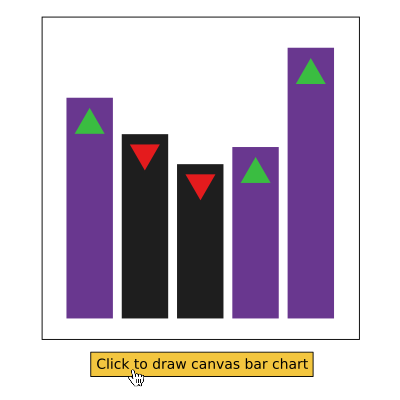
\includegraphics[trim={0.1cm 0.1cm 0.1cm 0.1cm},clip,width=0.58\textwidth,height=0.36\textheight]{testability/figures/motivating-example-new.png}
    \caption{An example canvas-based application. When the button is clicked, the plot is drawn dynamically (on the client side) using the canvas element.}
    \label{fig:motivating-example-1}
\end{figure}


Figure~\ref{fig:motivating-example-1} shows an example web application that uses canvas elements.
A bar chart is drawn in the canvas when the user clicks the button.
The corresponding JavaScript code is shown in Listing~\ref{lst:motivating-example-1}.
This example illustrates the dynamic nature of canvas-based web applications.
The data is plotted dynamically, on-the-fly, on the client side as opposed to the latency involved in sending the data to be plotted at a server that replies back with an image of the generated bar chart.
This dynamic nature makes canvas elements useful in interactive and high-performance visualizations and graphics.

Listing~\ref{lst:motivating-example-1} shows a snippet of how the setup and manipulation of canvas elements is done exclusively through the Canvas JavaScript API~\cite{w3c_canvas_standard}.
The canvas API provides functionality to draw lines, circles, rectangles, etc.
These can then be combined and dynamically added to the canvas element in order to draw more complex and interactive drawings.
Lines 6 to 11 show a snippet of how the canvas API is used to draw a rectangle on the chart.
A call is made to the \verb|fillRect()| function from the canvas API with parameters specifying the rectangle.
This allows dynamic creation of shapes on the canvas.

However, the HTML canvas element itself (Listing~\ref{lst:motivating-example-1}, lines 17-21)  remains empty throughout the entire usage of the application.
The execution of various canvas API functions does not change or update the contents of the canvas element tag.
\hl{This is because, as required by the official W3C standard~\mbox{\cite{w3c_canvas_standard}} of canvas elements, the canvas has no DOM representation. That is, the DOM subtree under a canvas node remains empty, and therefore its state remains unobservable. 
Instead, the canvas API functions are required to draw \mbox{\emph{directly}} to the raw monitor pixels buffer without the costly task of maintaining a DOM representation. This direct drawing allows canvas elements to achieve high-speed performance in order to enable dynamic and highly-interactive applications. }

Unfortunately, this DOM-free nature that enables the high-speed of canvas elements is also the reason why they are more difficult to test.
At any point during the execution of the application, the state of the canvas remains unobservable.
While one might conceptually think of gathering state information by tracking the call stack of the API calls, this would not be applicable to an exclusively visual API such as that of the canvas.
This is because the actual visual rendered canvas does not directly correspond to the calls made to its API.
For instance, calls could mistakenly visually override one another, or they might call the API with unintended arguments, resulting in a wrong visual result. 
A thousand canvas API calls (for example, draw the rectangle in the example, \emph{one point} at a time) can produce the same resulting visual state as one canvas call (a single call to \verb|fillRect|).
Consequently, we can see that it is difficult to assess what state is the canvas in at any given moment which makes it difficult to test canvas elements.

\hl{In this chapter, we propose an approach that makes canvas elements testable. That is, the goal is to 
provide developers with the fundamental capability of observing the canvas state and making assertions on it. However, the aim is not to provide a complete testing solution, but rather to enable the 
testing process itself, thereby improving testability. This approach visually analyzes the canvas screenshot, then creates a DOM tree representing the visual state of the canvas.
This makes it possible to test the canvas element using common DOM-testing techniques.
Finally, the developers would write their own tests, or could optionally use the automatically generated tests to check the visual objects of the canvas and their properties.}


\begin{lstlisting}[language={javascript},
float=tbp,
aboveskip=1.4em,
caption=JavaScript and HTML snippet of the canvas drawing in Figure~\ref{fig:motivating-example-1}., 
label={lst:motivating-example-1}]

function onButtonClick() {
	var canvas = document.getElementById("canvasBarChart
").getContext("2d");
	...
	canvas.beginPath();
	...
	// Example: this would draw one of the
	// rectangles in the bar chart.
	canvas.fillRect(leftCoordinate, topCoordinate,
					width, height);
	...
}


// The HTML portion of the app
<canvas id="canvasBarChart">
	// This tag remains empty throughout the usage of
	// the app, due to the lack of DOM representation
	// for canvas elements.
</canvas>

\end{lstlisting}
% !TEX root =  paper.tex

\section{Proposed Approach}\label{sec:approach}

\begin{figure}[t]
    \centering
    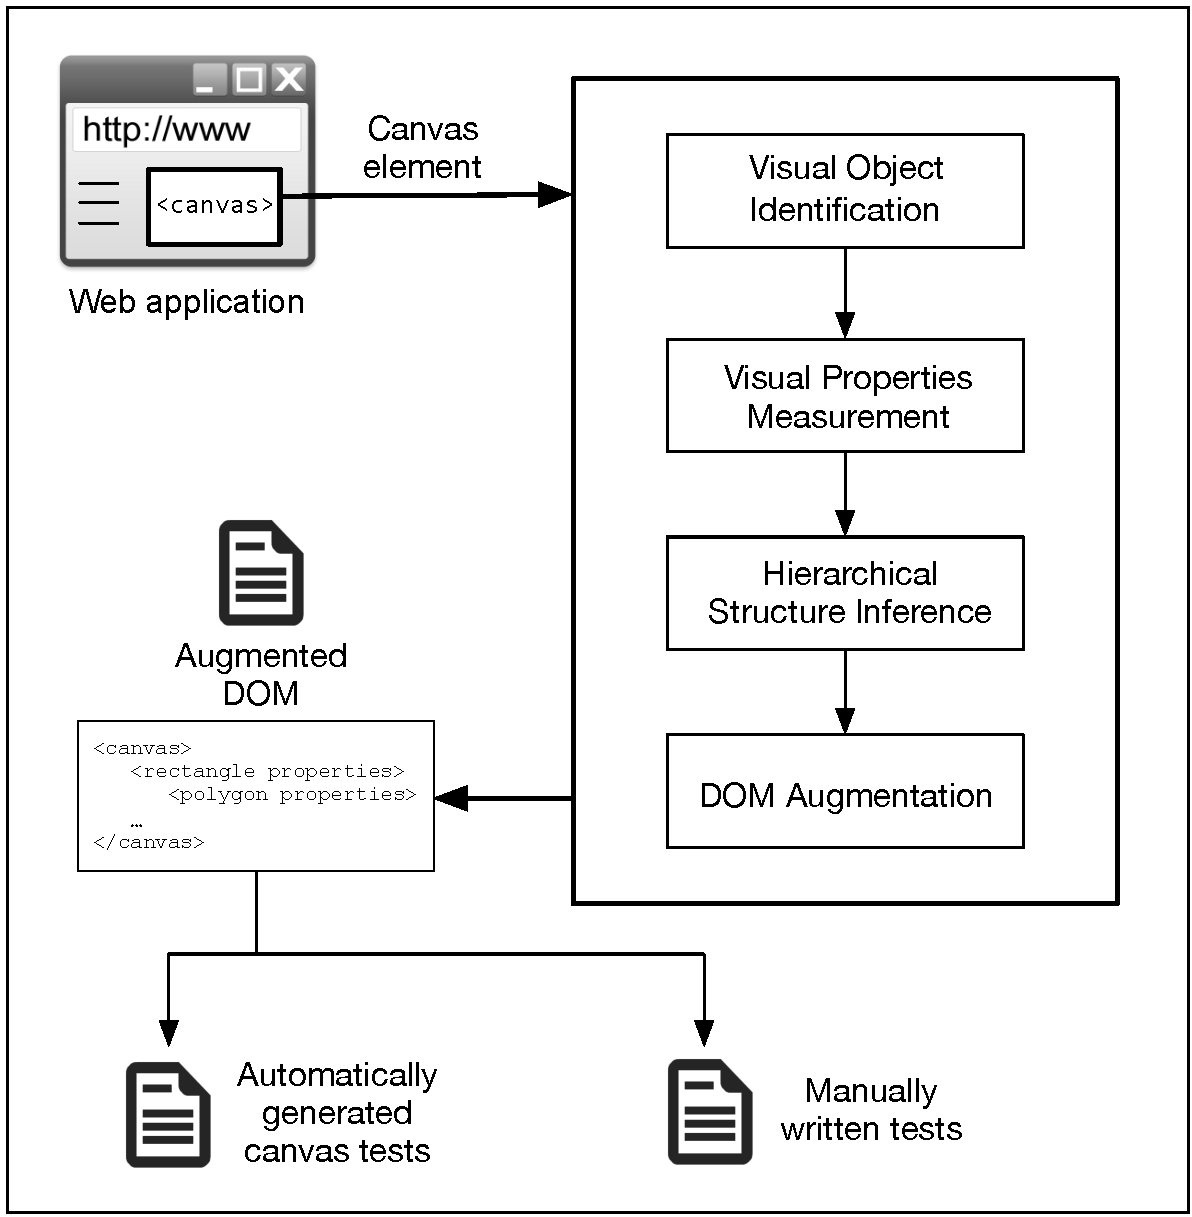
\includegraphics[trim={0.0cm 0.0cm 0.0cm 0.0cm},clip,height=7.9cm,width=0.62\textwidth]{testability/figures/canvasure-overview-figure.pdf}
    \caption{Overview of the proposed approach.}
    \label{fig:approach-overview-1}
\end{figure}

The approach starts by automatically opening the webpage containing canvas elements in an instrumented browser.
It focuses on canvas elements only and is therefore agnostic of the rest of the web application's page.
Therefore, it can analyze canvas elements contained in a larger webpage or canvas applications that are solely composed of a single canvas element.

\subsection{Overview}
Figure \ref{fig:approach-overview-1} depicts an overview of the main steps of the proposed approach.
For each canvas element on the page, a screenshot is captured and visually analyzed.
The visual analysis begins by performing a visual identification of objects on the canvas.
Our object identification is capable of identifying common geometrical shapes supported by the canvas API, such as lines, circles, and rectangles, as well as generic arbitrary shapes.
Next, the approach infers the visual properties such as color, size, and location, for each of the detected visual objects.
A list of all supported properties is shown in Table \ref{tbl:info-provided-by-approach}.
Subsequently, the approach builds a hierarchy information of the visual objects contained in the canvas.
This hierarchy information includes parent-child relations between objects, indicating which objects (if any) are contained inside other objects.
The hierarchy also includes z-order information, which indicates front-to-back arrangement of overlapping objects.

All the information extracted through the previous steps is then represented as an augmented DOM inside the canvas element.
The testing of the canvas is performed by generating assertions from the augmented canvas DOM.
We now describe each of these steps in detail in the following subsections.
 

\subsection{Visual Object Identification}
\label{subsec:viz-identification}
The objective of this stage is to detect and identify objects that are present on a canvas element.
We define an object to be present on the canvas if it is rendered and visible in the current screenshot of the canvas.
However, the approach does not require an object to be fully visible; occlusions and overlaps of multiple objects are allowed.
We apply a number of transformations on a copy of the original canvas image, $\mathbf{C_T}$, in this stage.

\head{Color contrast adjustment}
The goal of this first step is to perform a form of color contrast adjustment of the canvas screenshot.
This is performed in order to enable our analysis to \emph{see} objects more clearly. 

The analysis performs the color contrast adjustment through a \emph{color space conversion} of the canvas screenshot,  $\mathbf{C_T}$.
A color space conversion changes the representation of the colors of the pixels from one representation system to an alternative representation. 

We first need to select a suitable conversion method since several methods exist.
To that end, we perform an empirical examination of the eight most common conversion methods \cite{tooms2016colour}, namely HSV, L*a*b*, L*u*v*, CIE-RGB, XYZ, YUV, YIG, YPbPr, and YCbCr.
Each of these is simply a mathematical formula \cite{tooms2016colour} that changes pixels from one color representation to another. 

We empirically evaluate these conversions on a random set of 20 canvas elements.\footnote{http://corehtml5canvas.com} The results of this empirical examination are shown in Figure \ref{fig:param-est-colorspace}.
The figure shows how much contrast there is in the canvas image when using the different color conversions. The contrast is measured using 
the variance in pixel values. Higher values in the figure indicate  more contrast. Based on the results shown in the figure, the YCbCr conversion yields the best color contrast.
YCbCr will therefore be our choice for the color space that the canvas will be converted to.
Therefore, the algorithm creates a new image, $\mathbf{\bar{C}_T}$, which represents the canvas screenshot in YCbCr.
An example of the outcome of this step is shown in Figure \ref{fig:stages-examples}-a for a part of the motivating example.


\head{Detecting object boundaries}
The goal of this step is to detect the boundary of each object in the canvas.
This is performed in order to allow the analysis to roughly estimate where the objects are in the canvas image; this boundary information is used later to identify objects and their properties.

In order to detect these boundaries, we calculate the image gradient \cite{fernandez2012advanced}.
The image gradient is a mathematical processing applied on the canvas image to extract edges, which are the parts of the canvas where there is a transition from one object to another; for example, a boundary between an object and its background.

First, we need to select a suitable method to calculate the image gradient since several methods exist.
In order to be able to compute more accurate gradients for various canvas object shapes, we use the Scharr method \cite{scharr2000optimal}.
We make this choice because this method has been shown \cite{kroon2009numerical} to yield good results for smooth and curved objects in addition to angled objects.
 This would therefore be suitable for processing objects found on canvas elements.
  We compute the image gradient on $\mathbf{\bar{C}_T}$, and call it $\nabla \mathbf{\bar{C}_T}$.

Next, the analysis performs a binary transformation and converts each pixel in $\nabla \mathbf{\bar{C}_T}$ into either 0 or 1.
 A value of 1 represents a pixel that is on the object boundary, and a value of 0 means otherwise.
  The processed canvas image is called $(\nabla \mathbf{\bar{C}_T})^B$. 
To compute $(\nabla \mathbf{\bar{C}_T})^B$, we need to perform thresholding on the image, i.e., the reduction of a graylevel image to a binary image. 
We choose a machine learning clustering approach called Otsu thresholding from the computer vision literature, to perform this thresholding.
 Otsu's method is clustering-based and has been shown \cite{sezgin2004survey} to yield high performance. The outcome of this step is depicted in Figure \ref{fig:stages-examples}-b for the motivating example. 


\head{Separating objects}
So far, we have a collection of boundaries, but we do not know which group of boundaries belong together as part of the same object.
The goal of this step is to separate the different boundaries detected in the last step. 

\begin{figure}[t]
    \centering
    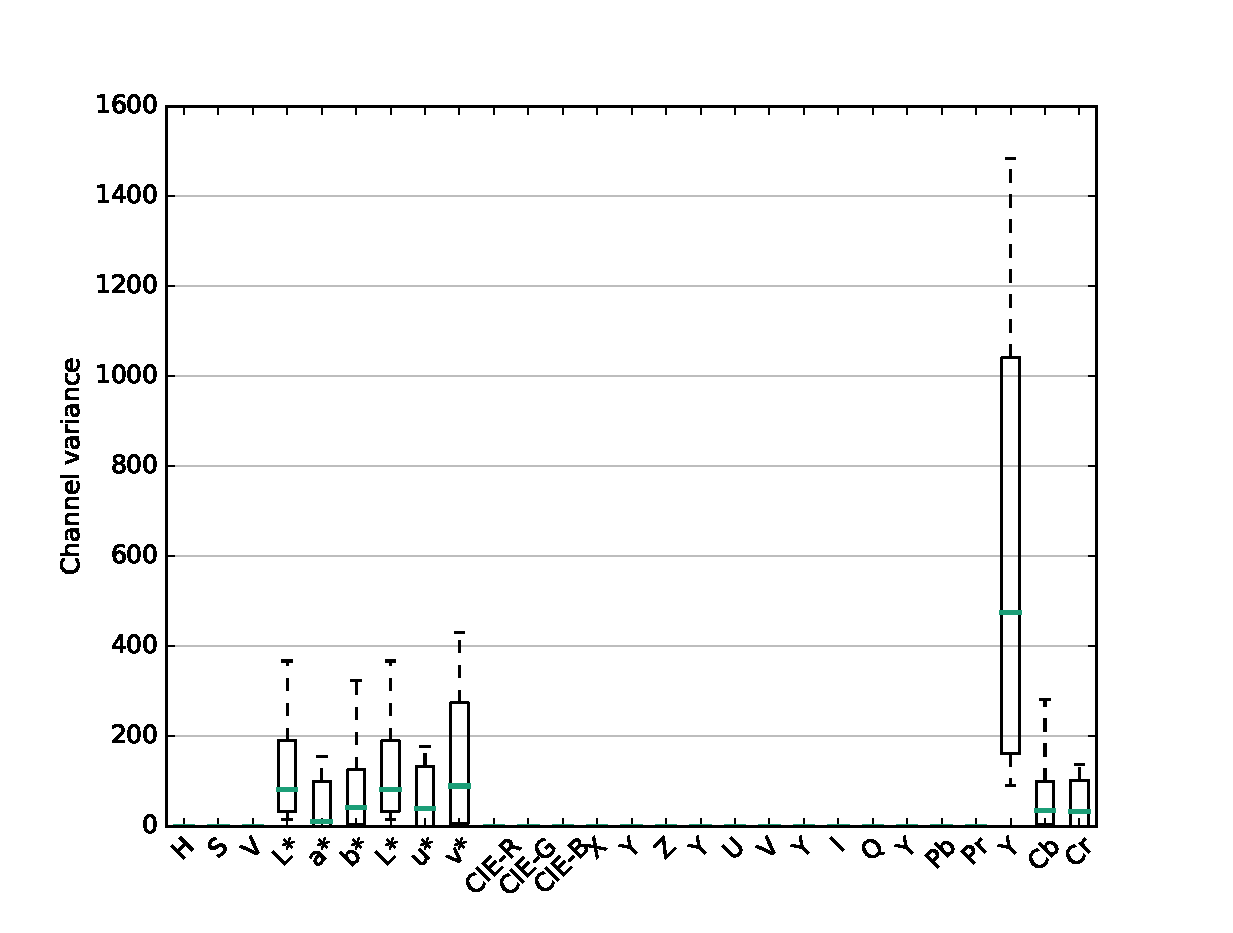
\includegraphics[trim={0.3cm 0.3cm 0.3cm 0.3cm},clip,height=0.35\textheight, width=0.74\textwidth]{testability/figures/colorspace-parameter.eps}
    \caption{Parameter estimation for the color contrast adjustment step of the algorithm. Choosing the YCbCr color representation yields best contrast adjustment for the canvas screenshot. Higher values are better. }
    \label{fig:param-est-colorspace}
\end{figure}



First, our analysis goes through the list of all detected boundaries. For each boundary, the algorithm walks on the boundary, step by step, and examines which other boundaries are connected to it. At the end of this process, we have a group of disjoint boundaries $\mathbf{B}_i$:
%\begin{align}
\begin{equation}
\label{eqn:approach-regions}
(\nabla \mathbf{\bar{C}_T})^B = \bigcup \mathbf{B}_i \,\, : \,\, \bigcap \mathbf{B}_i \equiv \O
\end{equation}
%\end{align}	
where $\mathbf{B}_i$ is a set containing the boundary pixels of the $i^{th}$ detected object in the canvas. The equation shows that each boundary $\mathbf{B}_i$ is separate from other boundaries, $\mathbf{B}_{j\neq i}$.

The algorithm then proceeds by computing the \emph{Euler number} \cite{sossa1996computation} for each boundary $\mathbf{B}_i$. The Euler number is a metric that shows whether a boundary has branches, or is a continuous boundary. For example, geometric shapes such as rectangles or circles have boundaries that continuously surround the shape without branching. On the other hand, two rectangles sharing an edge will have a branch in their boundary.

Next, the algorithm uses the Euler number $\mathcal{E}$ that was just computed in order to check for branching in a boundary. A value of $\mathcal{E} = 0$ indicates that the boundary is one continuous shape without branching. For this case, the algorithm saves the boundary as is without further modifications. On the other hand, a value of $\mathcal{E} < 0$ indicates that a boundary has branching. In this case, the algorithm breaks down the original boundary and creates new boundaries for each branching. We note that this will not cause 
any unnecessary or excessive fragmentation of the structure, 
because the fragmentation only occurs when the boundary branches, 
and no branching occurs for continuous (i.e., unbranched) segments 
of the object.  

At this stage, the analysis has extracted a set of boundaries $\mathbf{B}_i$ from the canvas image that are separate from each other and non-intersecting.  
An example of the outcome of this step is shown in Figure \ref{fig:stages-examples}-c.

\head{Extracting segments on boundaries}
The purpose of this step is to help identify the type of each object (e.g., rectangle, circle, arbitrary shapes, etc) based on extracted segments from its boundary. To this end, we take the object boundaries detected so far and break them into smaller line segments.  Objects that are curved and smooth, such as circles or generic shapes, are still represented by linear segments too, but as minuscule lines at a zoomed-in scale. While more complicated computer graphics models might be used (e.g., curves, polynomials), we opted 
for linear segments to simplify the analysis and make it faster. 

Following the detection of all boundaries $\mathbf{B}_i$, 
we need to understand what the \emph{identity} of each boundary is. 
This is because, at this stage, we only have a collection of boundaries but do not know what shapes do they represent, or 
what their properties are (e.g., dimensions, colors). 
The first step towards gaining this information is to segment these boundaries or break them down into smaller sections. 
Accordingly, the analysis proceeds by populating each boundary with a random set of probabilistic Hough segments from the computer vision literature \cite{matas2000robust}. These segments are small linear portions of the boundary of each region. This approach has been shown \cite{kiryati2000randomized} to produce robust extraction of boundary segments. In essence, this step performs rough clustering of boundary coordinates and groups neighboring points into a set of small segments.

The generated probabilistic segments are, however, often redundant duplicates, overlapping, and/or intersecting. 
This is because the aforementioned Hough segmentation process is stochastic in nature and while it is robust in most situations, its stochastic nature does cause to generate false positives. 
This presents a challenge in terms of identifying which segment is a true linear segment and which is redundant. 
As such, the set of all generated segments does not have a direct 1-to-1 correspondence to linear segments on the boundary.

We address this by performing a post-processing of the generated segments. Post-processing starts by creating an \emph{R-tree} index. An R-tree~\cite{hadjieleftheriou2008r} is a database structure that allows storing, querying, and retrieving data that is spatial in nature (e.g., locations, point sets). Our set of segments is also an example of such spatial data. Therefore, we insert the segments into an R-tree index in order to efficiently perform spatial queries such as finding intersecting segments or neighbors.
 
Accordingly, two sets of operations are performed on the R-tree index. The first operation consists of iterating through each line segment in the index and then querying the existence of other segments with full or partial spatial intersection. The second operation also iterates through each line segment in the index, but queries the existence of neighbouring segments instead of intersections.

For the first R-tree operation, the result of each iteration is a set of segments that are fully or partially intersecting. The algorithm then performs a pair-wise iteration over the intersecting subset. For a pair of line segments that are parallel, the algorithm removes the smaller segment if it is fully enclosed in the larger segment. Otherwise, in cases where the rectangles (which represent the bounding boxes of objects) are partially overlapping, the two parallel segments are merged into one new line segment, and then removed from the set.

\begin{figure}%[b]
    \centering
    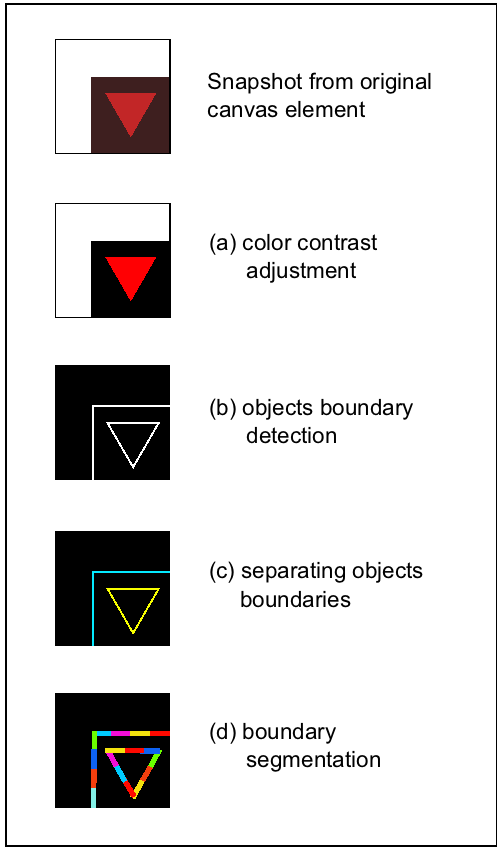
\includegraphics[trim={0.0cm 0.0cm 0.0cm 0.0cm},clip,height=7.5cm,width=0.35\textwidth]{testability/figures/stages-illustration.png}
    \caption{Illustration of the general stages involved in the visual identification of canvas objects. Best viewed on a color monitor. }
    \label{fig:stages-examples}
\end{figure}

For the second R-tree operation, the result of each iteration is a subset of segments that are neighbours of each other. The algorithm forms this subset by querying the R-tree index for the 4 spatial neighbours, one neighbour in each direction, around the query rectangle. The algorithm then performs a pair-wise iteration over the subset. Pairs that are both collinear and parallel are then merged into one new segment, and the forming segments are dropped from the set. Other pairs are left in the set as is.

%\begin{table*}[tb]
\begin{sidewaystable}
\setlength{\tabcolsep}{6pt}
\renewcommand{\arraystretch}{0.9}
\centering
\caption{List of the information that is visually inferred from the screenshots of web canvas elements}
%\begin{tabular}{lccc}
\begin{tabular*}{0.99\textwidth}{l @{\extracolsep{\fill}} ll}
\toprule
\textbf{Visual object identity} &  \textbf{Visual properties}  &  \textbf{Hierarchical structure} \\

\midrule
lines, triangles, rectangles,  &  - centroid: geometric center point of objects & - z-order: relative order of objects \\

squares, circles, & - size: & in the z-direction (i.e. behind or \\

generic shapes (polygons) & \, \, \, - width and height: for rectangles and squares & in front of other objects) \\

 & \, \, \, - diameter: for circles &  \\ 
 
* Note: our approach allows  & - color (HTML hex values) & - Parent-child relation: which \\

multiple overlapping, partially  & - orientation: number of degrees of rotation from horizon & objects are contained inside  \\

visible, or nested combinations & - point-set: the set of points representing generic shapes (polygons) & other objects. \\

of these objects. & & \\ 
 
\bottomrule
%\end{tabular}
\end{tabular*}
\label{tbl:info-provided-by-approach}
%\end{table*} 
\end{sidewaystable}


At this point, we have constructed a final set of line segments for each boundary. The analysis is ready to identify the shape type (e.g., lines, rectangles) of each object. An object whose set of segments has a cardinality of 1 is reported as belonging to the `line' type. Similarly, a set of three connected lines are triangles, and four lines are rectangles. For other objects, the analysis first performs an ellipse fitting to cover the object. Then, the relation between the major and minor axes of the ellipse is computed. If these axes are equal, then the detected shape is identified as a circle if the object's set of line segments has a cardinality of more than 4 (i.e. more than a rectangle) and its area is \emph{solid}. These set of conditions define what a circle is exactly. This is because a  region is defined as \emph{solid} when the the area of that region is identical to the area of the convex hull of the same region. On the other hand, when the region is not solid, the object is identified as a polygon.
Table \ref{tbl:info-provided-by-approach} lists the different object types recognizable by our approach. These types are the same types of objects provided by the canvas API. We note that our approach does not require any training dataset like machine learning approaches, because the attributes and identities of various shapes can be more precisely and robustly captured using mathematical ratios such as the process conducted in this step.
 
\subsection{Visual Properties Measurement}
\label{subsec:viz-props}

At this stage, our technique measures the visual properties of the objects detected in the previous section. These properties are extracted from the original canvas screenshot and include parameters such as location, size, and color. Table \ref{tbl:info-provided-by-approach} shows a list of the visual properties that are measured by the technique for the detected visual objects. This subsection describes the process by which we measure these properties.

\head{Object position} First, the technique calculates the centroid of each detected object. This is done by computing the arithmetic mean of all coordinates in the object. The centroid would therefore represent the point that minimizes the average Euclidean distance between itself and other coordinates in the object.

\head{Color} Next, for all coordinates in the object, the analysis computes the median pixel vector. This is performed to remove outliers that might be present due to small protrusions in the detected region. This vector is then assigned to the color property of the detected object.

\head{Size and orientation}
Subsequently, the analysis performs an ellipse fitting to the region of the object. The ellipse is centred on the centroid, and its axes are fitted so that the ellipse covers the entire object. By the end of this process, an ellipse is generated for each detected object, with each ellipse having a centre, a major axis, and a minor axis. The analysis then extracts a number of visual properties based on the fitted ellipse. First, if the shape is a rectangle, the ellipse axes determine the width and height because the ellipse's major and minor axes would align with the rectangle's axes. If the shape is a circle, then ellipse axes determine the diameter. Next, an orientation is assigned to the object. This orientation is computed as the angle between the major axis of the ellipse and the positive horizontal axis. This represents how much the object is rotated. 


\head{Point set}
Finally, the analysis extracts a representative point set for each object. This point set lists the coordinates necessary to reconstruct the object. This set is only generated for triangles and generic shapes (polygons), since other object categories are fully identified using their other measured properties, as shown in Table \ref{tbl:info-provided-by-approach}. 
In order to generate this representative point set, the analysis takes as input the coordinates of the object boundary and then proceeds to apply the \emph{Harris} operator for the computer vision literature \cite{ryu2011formula}, which is a mathematical transformation that detects points of intersections in boundaries. This process extracts points with more than one directions of lines coming in/out of it, which yields points where linear segments intersect. 
 
\subsection{Hierarchical Structure Inference}

For each detected canvas object, the analysis then performs a sequence of operations on the canvas screenshot that we have processed so far in order to infer any hierarchical information. We define hierarchical information as the information pertaining to the relative spatial relations between overlapping or nested objects. Objects that are not overlapping or nested have no hierarchical information.

More specifically, the hierarchical information of an object has two parts: the z-order and the parent-child relations. 
The z-order determines the relative arrangement of overlapping objects along the z-axis (i.e., front to back arrangement). While the width of the screen is represented with an x axis and the height of the screen represented by a y axis, the z-axis is perpendicular to the xy screen plane and points towards the user. That is, it determines which objects are closer to the viewer and away from the screen, and which are away from the viewer into the screen. 

The second part of hierarchical information is the parent-child relations.
This hierarchical information examines nested objects and determines which are children objects and which objects are their parents.
We define object A to be a child of object B if object A is entirely visually contained inside object B.
Equivalently, object B is a a parent of object A if it entirely contains it.
Objects that are not fully contained in other objects (for example, in cases of partial overlaps) are siblings, and do not have a parent-child relation.

The analysis starts the inference process by creating two directed acyclic graphs for the detected objects.
The first graph, $\mathbf{P}$, captures parent-child information.
The second graph, $\mathbf{Z}$, contains z-order information.
Every object is initialized as a degree zero vertex on the graphs.
Subsequently, the analysis creates an R-tree index. Each item in the index is a 2-tuple of a detected object and its minimum bounding rectangle. 

The analysis then iterates over the collection of detected objects.
For each object, the analysis performs a spatial query on the R-tree to determine the leaves that are intersecting with the object.
This results in one of three possible scenarios.
The first is when the R-tree returns no intersections with the object.
The second is when the intersecting object has its minimal rectangle fully inside the query object.
The third case is when the intersecting rectangles are partially overlapping.

For the first case, the minimal rectangles of the tree leaves are non-intersecting.
This query result indicates that there are no overlapping or nested objects with the current object.
As such, the object has no defined hierarchical information.
The $\mathbf{P}$ and $\mathbf{Z}$ graphs are therefore not updated, and the corresponding vertices of the object remain in their initial state of zero degree.

For the second case, the query indicates that one or more objects are fully contained inside the query object.
Therefore, this constitutes a parent-child relation.
Accordingly, we update both graphs $\mathbf{P}$ and $\mathbf{Z}$.
The update to $\mathbf{P}$ is a new directed edge from the child to the parent.
Similarly, the update to $\mathbf{P}$ is also a directed edge from the child to the parent.

Finally, for the last case, the query returns a partial overlap of the minimal rectangles.
As such, this case would not constitute a parent-child relation.
However, it is still possible for this case to have z-order relations.
Accordingly, the analysis proceeds to detect the presence of a z-order relation.
First, the analysis generates the concave parts of the region.
These parts are the subtraction of the convex hull of the region from the original region.
Next, the analysis performs an element-wise logical XOR between concave parts of the object and the objects with the partially overlapping minimal rectangles.
If the result of the operation is a non-zero region, then a z-order relation exists.
The analysis proceeds by creating a directed edge in $\mathbf{Z}$ from the object with the concave parts to the object that is resulting from the R-tree query.


\subsection{Testing through DOM Augmentation}
\label{subsec:testing-using-dom}
At this stage, the analysis has concluded the process of building information about the identity, properties, and hierarchical structure of the objects on the canvas. The analysis proceeds by casting this information into a DOM tree and augmenting it to the original canvas element.

\head{DOM Augmentation}
First, the analysis creates a DOM node for each detected object on the canvas. The tag name of the node matches the identity of the object. For example, an object that has been identified as a triangle is represented as \verb|<triangle>|, generic shapes (polygons) as \verb|<polygon>| and so on. 

Next, for each node in the DOM, the analysis inserts all the detected attributes pertaining to the identified object (see Table \ref{tbl:info-provided-by-approach} for a full list of attributes). For example, a \verb|diameter| attribute is added to each \verb|<circle>| node.

Finally, the analysis then proceeds by arranging the nodes of the DOM according to the inferred hierarchical information. We recall that the hierarchical information consisted of two parts: the parent-child relations contained in the $\mathbf{P}$ graph, and the z-order relations contained in the $\mathbf{Z}$. For the parent-child relation, the analysis re-orders the nodes of the DOM as to make child nodes in the DOM correspond to child objects on the canvas (as described in the hierarchical structure extraction section). The analysis then adds a \verb|z-order| attribute to each node. A z-order of zero indicates a front-most object, and elements further back have increasing negative values.

\lstdefinelanguage{HTML5}{
	language=html,
	alsoletter={-,=},
	otherkeywords={
		% HTML tags
		<html>, <head>, <title>, </title>, <meta, />, </head>, <body>,
		<canvas, </canvas>, <rectangle, </rectangle>, <triangle, </triangle>, <script>, </script>, </body>, </html>, <!, html>, <style>, </style>, ><
	},  
	ndkeywords={
		% General
		=,
		% HTML attributes
		charset=, id=, center=, color=, z-order=, point-a=, point-b=, point-c=,width=, height=,
		% CSS properties
		border:, transform:, -moz-transform:, transition-duration:, transition-property:, transition-timing-function:, z-order=
	},
	morecomment=[s]{<!--}{-->},
	tag=[s]
}

\begin{lstlisting}[language=HTML5,float=*,caption={The visually inferred augmented DOM for the canvas element of the motivating example (Figure \ref{fig:motivating-example-1} and Listing \ref{lst:motivating-example-1})}, label={lst:augmented-DOM-result}]
	<canvas id="canvasBarChart">
	
	<rectangle center="(191,43)" width="86" height="295" z-order="-1" color="#673C8C">
	<triangle center="(107,43)" point-a="(93,43)" point-b="(114,33)" point-c="(114,55)" z-order="0" color="#41A74D"/>
	</rectangle>
	
	<rectangle center="(166,264)" width="87" height="355" z-order="-1" color="#673B8C">
	<triangle center="(57,264)" point-a="(43,265)" point-b="(64,254)" point-c="(64,276)" z-order="0" color="#41A74D"/>
	</rectangle>
	
	... the rest of the generated DOM ...
	</canvas>
\end{lstlisting}

At this stage, the analysis has finished constructing an augmented DOM tree for the canvas element. An example is shown in Listing \ref{lst:augmented-DOM-result} representing the generated augmented DOM corresponding to the motivating example. As shown in lines 4 and 8 of the listing, a triangle node is located inside a rectangle node in the DOM. This corresponds to the state of the original canvas in Figure \ref{fig:motivating-example-1}, where one can see that a triangle is visually located inside a rectangle.


\head{Testing process}
The proposed canvas DOM augmentation approach was designed to extend and enable the use of DOM testing techniques with canvas elements. As such, it can be used in any testing process that is based on the DOM. For example, through browser automation using Selenium, a test can be written to navigate to a page, click a few buttons, and then finally, through the proposed augmentation approach, assert that the canvas has a vertical red rectangle, for instance. This is similar to the common task performed in DOM tests when the presence of a certain element, say a \verb|<div>| with a certain id, is asserted. 

The inferred augmented DOM is then used to test the canvas element in one of two ways. In the first testing approach, a list of assertions can be automatically generated by default to assert the presence of all nodes of the DOM and their attributes and hierarchy, as shown in Listing \ref{lst:generated-tests}. The generated assertions are broken down into three types of assertions that correspond to the information inferred from the canvas: (a) assertions on the identity of objects, (b) assertions on the properties of objects, and (c) assertions on the hierarchy of objects. The reason for separating assertions into three different layers is twofold. First, this enables pinpointing the cause of assertion failures, as opposed to writing one assertion that asserts the state of the entire canvas as a whole. Second, this strategy gives the user a flexible way of choosing which aspect of the canvas to test. For instance, the user can indicate that they are only interested in testing the presence of objects on the canvas, regardless of position or color. Of course, the user can keep the default option where all attributes are tested. Therefore, instead of just simply reporting that a test has failed, the approach, for example, can report that the test has failed because a triangle was absent or has changed color in the canvas.

Alternatively, in the second testing approach, the augmented DOM can be used in a case where a tester would write specific tests to assert the existence of particular objects, properties, or certain hierarchies of interest. %This would then only test the assertions specified by the tester. 
This use case would, therefore, be more appropriate for scenarios such as test-driven development, for instance.
However, we emphasize that the goal of the proposed approach 
is to provide developers with the \emph{ability} to test canvas elements, since they are not testable at the moment. That goal is the priority, more so than providing a complete end to end testing 
solution that would cover all the possible ways or markups 
that developers would prefer to write their tests in. 

     \begin{lstlisting}[language=Java, float=*, caption={The automatically generated test assertions for the canvas element of the motivating example (Figure \ref{fig:motivating-example-1} and Listing \ref{lst:motivating-example-1})}, label={lst:generated-tests}]
// High-level test: testing the identity of objects in the canvas
 assertTrue("'canvasBarChart' should contain 5 triangles",
   webDriver.findElements(By.xpath("//canvas[@id='canvasBarChart']//triangle")).size() == 5);

 assertTrue("'canvasBarChart' should contain 5 rectangles",
   webDriver.findElements(By.xpath("//canvas[@id='canvasBarChart']//rectangle")).size() == 5);
   // ...

// More detailed test: testing the locations of objects in the canvas
 assertNotNull("'canvasBarChart' should contain a triangle at (107,43)",
   webDriver.findElement(By.xpath("//canvas[@id='canvasBarChart']//triangle[@center='(107,43)']")));
	// ...

// More detailed test: testing the size of objects in the canvas
 assertNotNull("'canvasBarChart' should contain a rectangle with width=86 and height=295",
   webDriver.findElement(By.xpath("//canvas[@id='canvasBarChart']//rectangle[@width='86' and @height='295']")));
	// ...

// ... Tests for other properties (z-order, color, etc)
     \end{lstlisting}
	

\header{Implementation}
We implemented our canvas visual inference approach in a tool called \tool\cite{canvasure}. \tool is implemented in Python 3. We use the numpy~\cite{walt2011numpy} library to import basic mathematical and numerical functions, and use the scipy~\cite{jones2014scipy} library for matrix computations on the screenshots. We use the Selenium web driver to run and instrument web applications and extract canvas elements.



% !TEX root =  paper.tex

\section{Evaluation}\label{sec:evaluation}

In order to assess the accuracy and effectiveness of \tool, we examine the following research questions:

\begin{description}
\item[RQ1:] How accurate is \tool in visually inferring canvas elements and their properties?

\item[RQ2:]  How effective is \tool in detecting faults in canvas elements?
\end{description}

\subsection{Subject Applications}\label{sec:subjects}
Our main criterion for selecting subject applications was the central role of canvas elements in the function of the application. 
More specifically, the applications should either be entirely canvas-based, or use canvas elements as the main and central display of information. The rationale for this criterion is that we found 
some instances were the subject was not a canvas-based application, 
but rather only used small (e.g., icon-sized) canvas elements to display icons, and therefore this does not represent a canvas element that is rich and complex enough to be fairly included in the evaluation. We note that our approach is agnostic to the rest of the web application and can therefore process a single canvas element on its own or canvases that are central displays of the entire application.
Using this selection criterion, we were able to collect five open-source applications that use canvas elements. A list of these applications is shown in Table \ref{table:eval-apps}. As can be seen in the list, the applications cover a variety of sizes, ranging from between 7,200--105,000 lines of code. The applications cover a variety of domains, including graphics, medicine, chemistry, and music.

\begin{table}[b]
\setlength{\tabcolsep}{6pt}
\renewcommand{\arraystretch}{0.9}
\centering
\caption{List of web applications used for evaluation}
\begin{tabular}{llr}
\toprule
\textbf{Application} &  \textbf{Description}  &  \textbf{LOC}  \\
\midrule
JBrowse~\cite{eval_app_jbrowse} & Genome browsing and visualization & 105,427 \\
Reactome~\cite{eval_app_reactome} & Reactions analysis & 27,702 \\
Scribl~\cite{eval_app_scribl} & Genetics analysis & 20,939 \\
Gibberish~\cite{eval_app_gibberish} & Music composition and production & 14,884 \\
iCanplot~\cite{eval_app_icanplot} & Data plotting and visualization & 7,269 \\

%&                        &                 & \bf{\# tested} \\ 
%&  \textbf{Description}  &  \textbf{LOC}   & \bf{canvases}  \\
%\midrule

\bottomrule
\end{tabular}
\label{table:eval-apps}
\end{table}

\subsection{Experimental Procedure}
\label{sec:experimental-procedure}
\head{Accuracy: RQ1}
Through RQ1, we aim to evaluate the accuracy of \tool in visually inferring objects from the canvas. This is important in order to ensure  the inferred augmented canvas DOM exhibits a faithful representation the visual canvas.
To this end, for each subject application, we collect a random sample of 10 canvas screenshots, for a total of 50 screenshots of canvases from the 5 subject applications. Before the screenshots of the canvases are taken, the code temporarily makes all non-canvas elements invisible, such as advertisement boxes or other superimposed areas, in order to make sure that the snapshot is specific to the canvas element. We also note that the number of canvas elements is not that same for all subject applications, or at different points throughout the use of the same application. As such, when conducting the evaluation, by temporarily hiding all non-canvas elements the screenshot is taken from the page without specifying the canvas element. In a production environment, the developer would of course have the option, if needed, to specify which element to test. 

We then generate the augmented canvas DOM for each collected canvas screenshot. Subsequently, we recreate a canvas by rendering an image from the structure and properties in the augmented canvas DOM. Finally, we compare the similarity between the snapshot of the original visual canvas element, and the canvas image created from the augmented canvas DOM.

We compute the accuracy as a normalized root-mean-square (RMS) error $\Delta E$ in order to obtain a normalized similarity score to enable comparison across subjects. This accuracy measures the pixel-by-pixel similarity between $C_O$, the original canvas screenshot image, and $C_{DOM}$, the canvas image reconstructed from the augmented DOM. We compute this accuracy measure as follows:
\begin{align}
\label{eqn:eval-RQ1}
\Delta E = 1 - \frac{\sqrt{ \frac{1}{n} \sum {\left( C_{DOM} - C_O \right)}^2 }}{\Vert \left( C_{DOM} - C_O \right) \Vert_2}
\end{align}
a $\Delta E$ value of 1.0 (i.e., 100\%) indicate high accuracy (an identical match), while lower values indicate lower accuracy. 

\head{Effectiveness: RQ2}
The objective for addressing RQ2 is to assess the effectiveness of the tool in terms of its fault detection ability. To this end, for each collected canvas screenshot, we run \tool to infer the augmented canvas DOM. Subsequently, we inject random modifications into these canvas screenshots and generate another augmented canvas DOM. This process would therefore yield two DOMs: an original pre-injection DOM, and a post-injection DOM.

The fault injections take the form of injecting a random shape with a random set of points and random attributes (e.g., color, size, etc) directly on the canvas screenshot. The rationale for this fault injection model is to have the same degree of randomness across all evaluated applications, which can be difficult to ensure due to the following factors. First, the API of each subject application has varying degrees of being able to mutate the final visual state of the canvas. For example, some allow direct modification of the final visual content on the canvas, while for other applications the API allows only one or two properties to be changed. Furthermore, 
from a more practical point of view, we do not have access to the objects on the canvas due to the lack of observable state in the canvas, which is the very problem that our approach is trying to solve. Accordingly, due to absence of access to canvas objects, simulating a fault of removing a certain object is not practically achievable. Finally, the percentage of code contributing to the canvas visual state varies across subject applications. In other words, some applications have a large core of business logic code relative to only a small part of codebase for canvas drawing, while for other applications the code is almost purely visual code for canvas drawing. Accordingly, these differences add a confounding factor to the evaluation and skew the accuracy in different applications relative to others. We therefore adopt the fault injection approach outlined above in order to have a more unbiased evaluation.  

We therefore proceed as follows. We begin with the 50 canvas screenshots collected from the 5 subject applications. For each screenshot, we perform two injection runs, with one automatic random injection per run. Therefore, we end up with a total of 100 random injections for the 50 canvas screenshots collected from the 5 subjects.

The fault detection performance is then measured using the Jaro-Winkler~\cite{winkler2006overview} similarity $\Delta S$ between the pre-injection DOM and post-injection DOM. We chose this metric because it provides a normalized score, which would facilitate comparison and reasoning about results. For the purposes of this evaluation, we use the DOM instead of test assertions for two reasons. First, the DOM is the source against which any assertions are made, whether automatically or manually-written (as explained in section \ref{subsec:testing-using-dom}). We therefore evaluate the fault detection performance more accurately by checking the source DOM itself. Second, using a canvas assertion for this evaluation would introduce a bias as it requires a subjective human evaluation of whether a true positive or false positive actually occurred (e.g. does this object actually look bigger than before?). For these reasons, we perform a direct DOM distance comparison to avoid these biases and conduct a more accurate quantitative evaluation. We note that we are only able to perform this step after 
having evaluated that the generated DOM itself does faithfully 
capture the canvas state, and therefore the DOM distance comparison in this second stage of fault detection would faithfully capture incomplete or wrong canvas states.   

Accordingly, we define a true positive result and a false negative result using the Jaro-Winkler similarity $\Delta S$ between the pre- and post-injection DOMs. A true positive is defined as the case when the tool detects the injection. A false negative is defined as the case when it does not detect the injection. A false negative corresponds to $\Delta S \equiv 1$, where the pre- and post-injection DOMs are identical. Alternatively, a true positive corresponds to $\Delta S < 1$, where a difference was detected between the DOMs.


% !TEX root =  paper.tex

\subsection{Results and Discussion}\label{sec:discussion}

\begin{figure}[t]
    \centering
    \includegraphics[trim={0.3cm 0.3cm 0.3cm 0.3cm},clip,height=7.9cm, width=0.72\textwidth]{testability/figures/DOM-boxplot.eps}
    \caption{Accuracy of the inferred augmented DOM for each evaluated application in table \ref{table:eval-apps}. A total of 50 canvas elements in five different applications where used for this experiment.}
    \label{fig:result-DOM-accuracy}
\end{figure}

\head{Accuracy}
Figure \ref{fig:result-DOM-accuracy} shows box plots for the accuracy of \tool. 
The x-axis shows our subject applications, and the y-axis shows the  similarity percentage between the original canvas and the canvas regenerated from the inferred augmented canvas DOM. The runtime average for the tool is relatively fast at around 4 $\pm$ 0.3 seconds.

We make a number of observations from Figure \ref{fig:result-DOM-accuracy}. First, we note that most inferred DOMs have an accuracy close to or above $90 \%$ (the average for the dataset is $91.2 \% \pm 1.3$). Furthermore, at the highest and lowest of outliers, the accuracy ranges between $98 \%$ and $85 \%$. Therefore, we conclude from these results that the DOM inference process is relatively accurate in representing the canvas.

As for the accuracy at the lower end of the outliers, the reason for this is the inability of the probabilistic Hough transform used by the algorithm (as described in section \ref{sec:approach}) to generate segments to cover the small boundaries of small objects. These often take the form of small appendages connected to various objects, and the probabilistic Hough transform misses such small appendages. In a future version of the algorithm, we plan to improve the performance by finding a more suitable alternative than the probabilistic transform.

\head{Effectiveness}
Table \ref{tbl:result-fault-injections} shows the effectiveness results for \tool. 
Each row shows the total number of faults injection performed on the application, and then the number of true positives and false negatives reported by \tool, as described in section \ref{sec:experimental-procedure}.

From Table \ref{tbl:result-fault-injections}, we note that the overall rate of detecting true positives is $93\%$ and the overall rate of false negatives is $7\%$. Furthermore, we note that the per-application true positive rate varies from 16 out of 20 ($80\%$, lowest) to 20 out of 20 ($100\%$, highest). 
As such, we conclude from these results that the approach is relatively reliable in detecting faults in canvas elements. 

The main reason for the false negatives is that the probabilistic Hough transform used by the algorithm was unable to generate segments that would cover some of the injected shapes that were small appendages to other objects and this resulted in no modification to the segments set of the object. This is therefore reflected as a false negative. As part of our future improvements, we would like to improve the true positives rate even further by finding a better alternative to the probabilistic transform.

\begin{table}[b]
\setlength{\tabcolsep}{6pt}
\renewcommand{\arraystretch}{0.9}
\centering
\caption{Results of detecting fault injections}
\begin{tabular}{lccc}
\toprule
\textbf{Application} &  \textbf{\# Injections}  &  \textbf{\# True Positives} & \textbf{\# False Negatives} \\
\midrule
JBrowse~\cite{eval_app_jbrowse}      & 20 &  18  &  2 \\
Reactome~\cite{eval_app_reactome}    & 20 &  20  &  0 \\
Scribl~\cite{eval_app_scribl}        & 20 &  16  &  4 \\
Gibberish~\cite{eval_app_gibberish}  & 20 &  19  &  1  \\
iCanplot~\cite{eval_app_icanplot}    & 20 &  20  &  0 \\
\midrule
Total:  & 100   &  $93 \%$ &  $7 \%$ \\

\bottomrule
\end{tabular}
\label{tbl:result-fault-injections}
\end{table}

\head{Threats to Validity}
Our choice of subject applications could be a source of external threat to validity. In order to mitigate this threat, we select subject applications from a wide range of complexity (from around 7,000 to more than 100,000 LOC), and also select the applications from a varying assortment of fields, such as medicine, music, and chemistry. Another related threat is the relatively low number (five) of evaluated subjects. We mitigate this threat by extracting a random collection of 50 canvas snapshots for these applications and running 100 fault injections. \hl{Furthermore, some aspects in the fault injection process could be a source of internal threat to validity. There is currently no compilation of the types of faults that exist for canvases. Accordingly, 
in order to mitigate this threat and have an unbiased fault injection process, we chose to inject random shapes into the canvas. 
We also adopt a uniform approach of consistently injecting random objects on the canvas regardless of the applications's API, as opposed to individually injecting faults by modifying the specific API parameters of each canvas app. This helps in ensuring equally random fault injection across subjects. 
Furthermore, and perhaps most importantly, we do not have access to the objects on the canvas due to the lack of observable state in the canvas, which is the very problem that our approach is trying to solve. Accordingly, due to absence of access to canvas objects, simulating a fault by removing a certain object is not practically achievable.} Another related threat is the possible bias in the determination of true positives or false negatives. We mitigate this threat by injecting faults across all trials and then using a quantitative distance metric with a normalized range to allow a direct binarization of results into true positives and false negatives. 

Another potential threat to validity is the issue of cross-browser compatibility. We note that the rendering of canvas elements is categorically different from rendering regular web pages. When rendering a page, the browser has to continuously maintain a DOM and regularly recompute layout position and visual properties of the page elements before rendering. For canvas, however, the browser does not maintain any layout information about the canvas, and simply paints the pixels from the API call directly on screen. All browsers relay the pixel-by-pixel rendering directly to the canvas. Canvas elements have no observable state and browsers do not participate in maintaining what does or does not get rendered. This is the opposite of rendering webpages.

To the best of our knowledge, there is no evidence in the literature of cross-browser incompatibilities for canvas elements. Furthermore, in a recent study \cite{bajaj2014mining} categorizing questions asked by developers on StackOverflow, canvas related questions were mostly about how to use the canvas API. There was no reported pattern of questions on canvas-related cross browser incompatibility issues. In addition, and more importantly, from our own use and testing of canvas elements, we did not notice incompatibility issues either. For these reasons, we do not consider cross-browser incompatibility to be a threat to the validity of the proposed approach.



\section{Related Work}\label{sec:relatedwork}

There has been little to no research in the literature regarding testing canvas applications. Due to the absence of an object model for canvas elements, it is difficult to apply conventional web testing techniques to canvas elements.

Nonetheless, there exist a few open-source attempts, which can be used to perform  basic testing of canvas elements. However, these open-source tools are not part of a research publication, and therefore they lack detailed experimentation or a thorough explanation of the methodology. We briefly discuss some of these tools. 

Canteen\footnote{https://github.com/platfora/Canteen} takes a callstack analysis approach. The tool captures a stack of the function calls sent to the canvas element, then compares the runtime stack against a known correct call stack manually provided by the developer. A major disadvantage of this approach is that it focuses exclusively on the call stack, meaning a test's pass or failure does not directly correspond to the visual state of the canvas. That is, the actual rendered canvas that the end user observes is not tested.

Other open-source tools, such as Needle\footnote{https://github.com/bfirsh/needle} and JS-ImageDiff\footnote{https://github.com/HumbleSoftware/js-imagediff}, adopt a visual approach instead of code analysis. Runtime screenshots are compared against known good screenshots provided by the test writer. However, being a direct image differencing approach, it shares much of the fragility issues~\cite{coppola_automated_2016, leotta_visual_2014} of visual approaches, where even a single pixel could result in test failure. Furthermore, this approach still requires test writers to provide \textit{a priori} visual oracles.

There is another related body of literature that is related to visual-based approaches for testing web pages in general, but not for canvas testing. For example, WebDiff~\cite{choudhary2010webdiff} detects cross-browser incompatibilities for a given webpage. It performs an indirect comparison of the appearance of the webpage in two browsers using DOM-based analysis. Although the tool subsequently confirms the initial DOM-analysis using a visual comparison, the approach still requires the DOM to detect the cross browser incompatibility in the first place, and uses a visual comparison as a confirmation. Although the tool was shown to be helpful in terms of general web page cross-browser testing, it cannot be used with canvas elements because they lack a DOM representation. 

Another approach, using the WebSee~\cite{mahajan16apsec} tool, targets the problem of detecting and locating visual inconsistencies in web applications. The approach uses visual comparison to detect visual differences between pages, and then locates the inconsistency using DOM elements. While the approach showed good performance in detection and localization of inconsistencies, it does require the DOM in its operation and therefore can not be used with canvas elements.

PESTO~\cite{leotta2015automated} aims at simplifying the creation of visual web tests. The approach starts with a given DOM-based test suite and then generates visual locators. It then concludes by generating a visual test suite that matches original DOM test suite. While it shows good performance, canvas elements can not be used with this tool because they do not have a DOM.

Scry~\cite{burg2015explaining} focuses at assisting developers in explaining and reproducing visual changes on a web page. It asks the developer to specify which webpage element to monitor, and then watches that element. Whenever the appearance of the element changes, the method stores the DOM and CSS of that element in order to determine the code changes that produced the appearance change. While this tool has interesting applications and could help explain appearance changes in a web page, it can not be used for canvas elements because it is based on analyzing the DOM of elements. Canvas elements, however, have no DOM-tree representation, which makes it incompatible with such DOM-based tools.


\section{Conclusions}
\label{sec:conclusions}

Web applications based on canvas elements allow the creation of dynamic graphics, interactive user interfaces, and scalable visualizations. However, there has been little to no research in literature in terms of testing canvas elements. This chapter proposed a testing approach, implemented in a tool, \tool, based on visual analysis of the screenshot of canvas elements, and generating an augmented DOM tree for the canvas element to allow making test assertions on it. We evaluated the accuracy of the proposed approach and its effectiveness in detecting faults injected in canvas elements. We found the inference process to be relatively accurate (around $91\%$ accuracy on average) with a true positive rate of $93\%$ in detecting fault injections. 
We note, however, that the goal of this work is to provide developers with the fundamental capability of observing the canvas state and making assertions on it. However, it does not provide a complete testing solution, but rather make it \emph{possible} to perform the testing process itself, thereby improving testability. As part of future work, a more through canvas testing solution can be provided such that it will cover more complex and resizable canvas elements, and generate the tests in a fashion that developers might prefer (e.g., using relative positioning in assertions). 


\chapter{Semantic web accessibility testing}
\label{chp:accessibility_testing}

%% !TEX root =  paper.tex

% \usepackage{cite}
% \usepackage{amsmath,amssymb,amsfonts}
% \usepackage{algorithmic}
% \usepackage{graphicx}
% \usepackage{subcaption}
% \usepackage{textcomp}
% \usepackage{xcolor}
% \usepackage{multicol} % \columnbreak
% \usepackage{balance}
% \usepackage{enumitem}    
%\usepackage[table]{xcolor}
%\usepackage{nohyperref}

\usepackage{xcolor}

\usepackage{tabularx} 
\usepackage{collcell}

% \usepackage[usenames,dvipsnames,svgnames,table,xcdraw]{xcolor}
% \usepackage[usenames,dvipsnames,svgnames]{xcolor}
% \usepackage{pgfplots}
% \pgfplotsset{compat=1.10}


\usepackage{booktabs}
\usepackage[caption=false,font=normalsize,labelfont=sf,textfont=sf]{subfig}
%\usepackage{cite}
% \usepackage{hyperref}
\usepackage{array}
\usepackage{threeparttable}
\usepackage{enumitem}    
\usepackage[greek,english]{babel}
\usepackage{ifthen}
\usepackage{xspace}
\usepackage{fancybox}
\usepackage{marginnote}
\usepackage{tcolorbox}
\usepackage{multirow}
\usepackage{mathtools}
\usepackage{algpseudocode, algorithm, algorithmicx}
\usepackage{color}
\usepackage{soul}
\usepackage{graphicx}
\usepackage{amsmath}
\usepackage{tikz}
\usepackage{cleveref}
\usepackage{hhline}
\usepackage{balance}

\usepackage{listings}
\usepackage{parcolumns}
\usepackage{cleveref}

\usepackage{array}

\usepackage{adjustbox}
\usepackage{flushend}
\usepackage[switch]{lineno}
\definecolor{light-gray}{gray}{0.95}
\newcommand{\code}[1]{\colorbox{light-gray}{\fontsize{9pt}{10pt}\texttt{#1}}}

\definecolor{circled-color}{gray}{0.15}
\newcommand*\circled[1]{\tikz[inner sep=.1ex,baseline=-.75ex] \node[circle,draw,color=white,fill=circled-color] {#1};}


\def\BibTeX{{\rm B\kern-.05em{\sc i\kern-.025em b}\kern-.08em
    T\kern-.1667em\lower.7ex\hbox{E}\kern-.125emX}}
\newboolean{showcomments}
\setboolean{showcomments}{true}
\hypersetup{draft,bookmarks=false}

\ifthenelse{\boolean{showcomments}}
{
	\definecolor{myyellow}{RGB}{255, 228, 26}
	\definecolor{myblue}{RGB}{50, 50, 220}
	\newcommand{\nb}[2]{
		{\sf
			\fcolorbox{myyellow}{yellow}{\scriptsize\textbf{#1}}%
			$\blacktriangleright$%
			{\color{myblue}\fontsize{7pt}{8pt}\selectfont\textbf{#2}}%
		}%
	}
}
{
	\newcommand{\nb}[2]{}
}


\newcommand{\Mo}[1]{\nb{Mo}{#1}}
\newcommand{\Ali}[1]{\nb{Ali}{#1}}


\usepackage{color}


\definecolor{editorGray}{rgb}{0.95, 0.95, 0.95}
\definecolor{editorOcher}{rgb}{1, 0.5, 0} % #FF7F00 -> rgb(239, 169, 0)
\definecolor{editorGreen}{rgb}{0, 0.5, 0} % #007C00 -> rgb(0, 124, 0)

\lstdefinelanguage{JavaScript}{
  morekeywords={typeof, new, true, false, catch, function, return, null, catch, switch, var, if, in, while, do, else, case, break},
  morecomment=[s]{/*}{*/},
  morecomment=[l]//,
  morestring=[b]",
  morestring=[b]'
}
\lstdefinelanguage{HTML5}{
        language=html,
        sensitive=true, 
        alsoletter={<>=-},
        otherkeywords={
        % HTML tags
        <html>, <head>, <form>, </form>, <div>, </div>, <p>, </p>, 
        <span>, </span>, <input, <textarea, </textarea>, <select, </select>, 
        <option>, </option>, <title>, </title>, <meta, />, </head>, <body>,
        <canvas, \/canvas>, <script>, </script>, </body>, </html>, <!, html>, <section>, </section>
        },  
        ndkeywords={
        % General
        =,
        % HTML attributes
        charset=, id=, width=, height=, type=, value=, checked
        % CSS properties
        border:, transform:, -moz-transform:, transition-duration:, transition-property:, transition-timing-function:
        },  
        morecomment=[s]{<!--}{-->},
        tag=[s]
}

\lstdefinelanguage{CSS}{
  morekeywords={background,color,display,justify,content,font,weight,border,size,padding},
  morestring=[s]{:}{;},
  sensitive,
  morecomment=[s]{/*}{*/}
}
\newcommand{\todo}[1]{\textcolor{magenta}{\nb{TODO:}{#1}}}
\newcommand{\header}[1]{\par\smallskip\noindent\textbf{#1.}}
\newcommand{\toolname}{\textsc{AxeForm}\xspace}
\newcommand{\html}{\textsc{HTML}\xspace}
\newcommand{\css}{\textsc{CSS}\xspace}
\newcommand{\javascript}{\textsc{JavaScript}\xspace}
\lstset{%
    % Basic design
    backgroundcolor=\color{editorGray},
    basicstyle={\linespread{1.0}\scriptsize\ttfamily},   
    frame=l,
    % Line numbers
    xleftmargin={0.75cm},
    numbers=left,
    stepnumber=1,
    firstnumber=1,
    numberfirstline=true,
    % Code design   
    keywordstyle=\color{blue}\bfseries,
    commentstyle=\color{darkgray}\ttfamily,
    ndkeywordstyle=\color{editorGreen}\bfseries,
    stringstyle=\color{editorOcher},
    % Code
    language=HTML5,
    alsolanguage=JavaScript,
    alsodigit={.:;},
    tabsize=2,
    showtabs=false,
    showspaces=false,
    showstringspaces=false,
    extendedchars=true,
    breaklines=true,        
    % Support for German umlauts
    literate=%
    {Ö}{{\"O}}1
    {Ä}{{\"A}}1
    {Ü}{{\"U}}1
    {ß}{{\ss}}1
    {ü}{{\"u}}1
    {ä}{{\"a}}1
    {ö}{{\"o}}1
}






% !TEX root =  paper.tex
\section{Introduction}
Web accessibility is the notion of implementing web apps  
in a fashion that allows programmatic access to 
software functionalities that are otherwise only 
perceivable through certain senses (e.g., visually). 
Accessibility has been sometimes dealt with as an 
afterthought or a nice to have optional feature, 
with many developers and companies 
ignoring it altogether \cite{vendome2019can,harper2012web}. 
However, as shown in Figure \ref{fig:population-plot}, millions 
of people around the globe have software-relevant disabilities and are impacted by web accessibility, or the lack thereof. 

Furthermore, accessibility is increasingly becoming a legal 
requirement ratified into laws in many countries.
For instance, in the United States, the Americans with Disabilities Act~\cite{law:ada} 
requires all government and public agencies, as well as certain businesses, 
to make all their software and information technology 
services accessible. 
Similar provisions are required by law under the European
Union's Web Accessibility Directive \cite{law:eu_accessibility}.
Figure \ref{fig:lawsuits-plot} shows the increasing number of lawsuits
filed in federal US courts against businesses for failing to provide 
accessibility accommodations.

Despite the increasing legal, economical, and human costs due to lack of 
accessibility, there has been little work in the 
software engineering research community to automate accessibility testing.
Eler et al.~\cite{eler2018automated} check for missing attribute fields or 
incorrect attribute values related to accessibility of web pages, an approach that is 
also used in a few patents~\cite{sap2019accessibility, breeds2014software}.
The bulk of existing work focuses on topics such as 
evaluating best practices for conducting empirical accessibility evaluations, 
such as manual checklist walkthroughs~\cite{braga2014applying} or enlisting
visually-impaired users as part of user studies~\cite{bayer2006accessibility}.
A number of open-source tools have been developed to conduct simple syntactic accessibility tests 
that only check a few attribute values in a web page. 
In an audit of 13 of such accessibility testing tools conducted by the United Kingdom
Government's Office of Digital Services~\cite{ukgov:audit:2018}, 
these tools found only 26\% of a known small set of accessibility violations
present in tested web pages.

\begin{figure}%[b]
	\centering
	\includegraphics[width=0.70\columnwidth,height=6.0cm]{accessibility_testing/figures/population-plot}
	% \hspace{1cm}
	\caption{Number of people with software-related disabilities in the United States
		and the European Union. 
		% To put the numbers in perspective, the number of people with impairments is
		% comparable to the population of entire countries. 
		(Data compiled from: \cite{stats:accessibility_population:US, stats:accessibility_population:EU})}
	\label{fig:population-plot}
\end{figure}

The aforementioned tools are based on conducting \emph{syntactic} checks, 
which are simple markup rules (e.g., any \code{a} element must contain a non-empty string) 
to check for a minimal level of accessibility. 
However, none of the aforementioned tools analyze key accessibility 
requirements related to the \emph{semantics} of a page, such as the high level page 
structure and the roles or purpose of various elements. 
It is these semantic aspects of a page that users with 
disabilities rely on the most while using web pages~\cite{2019users_survey}, but none 
of the existing tools test for. 
Accordingly, the high level semantic analysis of web accessibility has remained 
a manual and laborious time consuming process~\cite{bai2016evaluation,
acosta2018toward,brajnik2008comparative,abou2008web}.  
   
To that end, we propose an approach that 
automates testing of a subset of web accessibility 
requirements pertaining to high level 
semantic checks that have not been amenable to automation. 
The approach is based on a visual analysis of the web page, 
coupled with a few natural language processing (NLP) steps, 
to conduct a semantic analysis of web pages. 
This analysis first identifies major cohesive regions of a 
page, then infers their 
\emph{semantic role} or purpose within the page.
Subsequently, a conformance check is conducted that determines 
whether the markup of the page correctly corresponds to the inferred semantics.  
If the markup contains the same semantic information perceivable by sighted users, 
the page is deemed accessible. Otherwise, if semantic information of the page is 
perceivable only visually but not conveyed in the markup, 
the page would be flagged as failing the accessibility test 
and the specific reasons are reported.   
In this work, we focus on vision disabilities as opposed to other forms 
of disability (e.g., hearing). The rationale for this is twofold. 
First, the web is predominantly a visual medium where most of the 
information is accessed visually as opposed to other senses. 
Second, surveys have shown that vision disabilities are the most relevant 
to web users with disabilities~\cite{2019users_survey}.

This chapter makes the following main contributions:
\begin{itemize}
    \item A novel approach for automatically testing semantic accessibility 
    requirements, which is the first to address this issue, to the best of our knowledge.
	\item An implementation of our approach, available in a tool called \toolname.
    \item A qualitative and quantitative evaluation of \toolname in terms of its 
    inference accuracy and ability to detect accessibility failures. 
    The results show that it achieves an F-measure (harmonic average of precision and recall) of 87\% for inferring semantic groupings, and is able to detect accessibility failures with 85\% accuracy. 
\end{itemize}


\begin{figure}%[b]
	\centering
	\includegraphics[width=0.70\columnwidth,height=6.0cm]{accessibility_testing/figures/lawsuits-plot}
	\caption{Number of software accessibility lawsuits filed in US federal courts per year. The number of lawsuits increased by around 3800\% over the four-year period 2015-2018. (Data compiled from: \cite{stats:accessibility_lawsuits:US_1, stats:accessibility_lawsuits:US_2})}
	\label{fig:lawsuits-plot}
\end{figure} 
% !TEX root =  paper.tex

\section{Background and Motivating Example}
\Cref{fig:acc-testing-motivating-example} shows an example of
an inaccessible web page. 
In a quick glance at the rendered page in \Cref{fig:acc-testing-motivating-example}-(c),
a sighted user can immediately understand
the structure of the page and navigate their way through
the various contents of the page.
For instance, the user would immediately recognize 
that they can navigate to other areas of the web site 
through the navigation menu at the top 
(i.e., Home, News, FAQ). 

While this happens naturally and instantaneously for sighted users, 
that is not the case for non-sighted users. 
The page structure (e.g., the presence of a navigation bar at the top)
is \emph{communicated exclusively} through visual design, 
since the HTML markup in \Cref{fig:acc-testing-motivating-example}(a) 
is simply a collection of \code{<div>}s that do not communicate  
any semantic functionality. 
This implicit visual communication is intuitive and natural 
for sighted developers and users, but is unavailable 
for users who can not have \emph{access} to visual 
information due to disabilities. 
Accordingly, the markup is deemed \emph{inaccessible}, 
because it is expressed in a fashion that does not provide 
any semantic information about the page structure.  

\begin{figure*}%[h]
	\centering
    \noindent
    \begin{minipage}[c]{.4\textwidth}
        \centering
        \begin{lstlisting}[language={html},frame=ltbr,
            aboveskip=1.0em]
  <div class="nv8471">
  <div>Home</div>
  <div>News</div>
  <div>FAQ</div>
  <div>Contact</div>
  </div>
        
  <div class="_hd902">
  Resources
  </div>
  <div>
   ...
  </div>
  
  <div class="_hd902">
  About Us
  </div>
  <div>
   ...
  </div>
        \end{lstlisting}
    	(a) HTML markup
    \end{minipage}
%    \hfill
\  \  \  \  \  \ 
    \begin{minipage}[c]{.45\textwidth}
        \centering
        \begin{lstlisting}[language={CSS},frame=ltbr,
            aboveskip=1.0em]
.nav8471 {
   background-color:
    #ffff00;
   display:
    flex;
   justify-content:
    space-around;
   font-weight:
    bold;
   border:
    2px solid #000000;
}
._hd902 {
   font-size:
    5vw;
   font-weight:
    900;
   padding:
    8vh 0 2vh 0;
}
        \end{lstlisting}
    	(b) CSS declaration
    \end{minipage}
%    \hfill
    \begin{minipage}[c]{.85\textwidth}
        \centering
        \ \\ \ \\ 
        \fbox{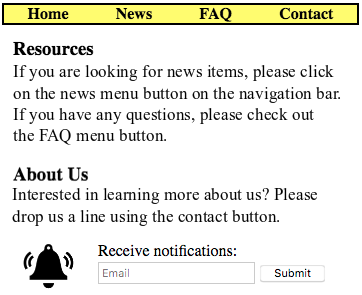
\includegraphics[scale=0.5]{accessibility_testing/figures/motivating-example/rendered-3.png}}
        \\ (c) Rendered page
    \end{minipage}
  
%    \begin{minipage}[c]{.6\columnwidth}\centering
%        (a) HTML code
%    \end{minipage}
%    \hfill
%    \begin{minipage}[c]{.5\columnwidth}\centering
%        (b) CSS declaration
%    \end{minipage}
%    \hfill    
%    \begin{minipage}[c]{.85\columnwidth}\centering
%        (c) Rendered page
%    \end{minipage}    
    \ \\ \caption{An example of an inaccessible web page.}
    \label{fig:acc-testing-motivating-example}
  \end{figure*}

The analysis and conclusion that we just made is currently 
being done manually, since it requires high level semantic analysis of the page. 
Our goal in this work is to automate the reasoning we have 
just described in order to be able to automatically 
reach conclusions about the accessibility of web pages. 


\subsection{ARIA  Roles}\label{subsec:aria-roles}
The aforementioned lack of semantic markup in the 
code makes it difficult for non-sighted 
users to navigate the page. This is because such users rely on 
\emph{screen readers} to parse the page for them 
and present them with the various information or navigation options present in the page. 
Screen readers are tools that speak out the various options, regions, or tasks accessible 
from the page, and the non-sighted user would then select one of the options they heard from 
the screen reader. 
Screen readers can be thought of as web browsers for non-sighted users, 
with one major caveat.
While a standard web browser simply renders the page as is and leaves 
it to the end user to understand what the various elements mean, 
screen readers expect that the page markup contains semantic information 
about various areas of the page, which the reader would then announce audibly, 
giving non-sighted users an understanding of the overall semantic structure of the page.

The standard that is used by screen readers during their processing of 
web pages is the W3C \emph{Accessible Rich Internet Applications} 
(ARIA)~\cite{ARIA} semantic markup.
The ARIA standard specifies a set of markup attributes that 
should be included in the page's HTML to make it accessible to screen readers 
or other assistive technologies. An example of such ARIA attributes is presented in the following subsection. 

\header{Targeted roles}\label{header:targeted-roles}
ARIA defines more than 80 attributes spanning various aspects of the page, 
from low level syntax requirements to high level semantic structure. 
We therefore have to target a subset of these ARIA attributes because 
addressing all 80+ attributes in a single academic work is untractable. 
The basis for selecting the targeted roles is that we focus on the most 
commonly used subset of ARIA, which are \emph{landmark roles}~\cite{2019users_survey}.  
Our own experimental results (\Cref{subsec:run-results}) also demonstrate the 
widespread use of these roles.
The roles identify the major high-level regions of the page and 
specify the semantic role for each of them.  
They consist of a set of specific pre-defined roles that convey, 
though markup, the otherwise only visually perceived role of each region.
For instance, the yellow rectangle at the top of \Cref{fig:motivating-example}(c) 
is perceivable as being a navigation bar, 
therefore the markup of the element containing that region has 
to include the landmark attribute \code{role="navigation"}. 
When a non-sighted user loads the page, the screen reader would read out loud (i.e., generated audible speech) the presence of a navigation bar (and any other semantic regions in the page), allowing the user to quickly perceive the high level structure of the page, and directly interact with the region they are looking for.

Accordingly, the absence of semantic markup in \Cref{fig:motivating-example}(a) 
makes the page inaccessible, because screen readers would be unable to 
provide alternative, non-visual, means of accessing the page.  
That is, the information and cues about the
structure and navigation of the page remain locked 
in the visual design of the page and can not be 
accessed non-visually.
When a web page communicates the important and key aspects of its structure and function using only visual design, without providing a programmatic means to access the same information, it is deemed inaccessible.

\subsection{Existing Tools: Syntax  Checkers}\label{subsec:syncheckers}
Existing accessibility testing tools~\cite{ukgov:audit:2018} are 
based on syntactic checking. 
They check the HTML against certain syntax rules. 
For instance, one common check is to assert that every \code{img} element 
has an \code{alt} text attribute (for text descriptions). 
Another check asserts that \code{input} elements must not 
be descendent of \code{a}.
Another example is checking that every \code{form} 
element has a \code{label} attribute.  
 
While such syntax checks can be useful simple 
assertions and are easy to automate, 
none of the existing tools perform the more important, 
and more challenging, high level \emph{semantic} 
analysis of the page's content. 
For instance, consider the subfigure (c) in \Cref{fig:motivating-example}, 
where we can see that there is a navigation bar at the top. 
Now consider the HTML in subfigure (a), where we observe that 
the developer did not use the required ARIA attribute 
of \code{role="navigation"}. 
Accordingly, because we visually see a navigation region in (c) 
but do not find it expressed in the markup in (a), 
we conclude that the page has an accessibility failure, 
because we perceived a certain semantic structure as sighted users, 
but it was not expressed in the markup in order to ensure it would 
be equally available for non-sighted users. 
That is the the \emph{central} issue in accessibility: 
making sure that whatever is visually perceived 
is also expressed in the code. 

We now pause to reflect and observe that there is no syntactic check 
that can automate the conclusion we just reached. 
That is, the process that we just walked through requires 
our own visual perception as humans in order to reach the conclusion 
that there is a mismatch between the perceived page and the markup. 
This process cannot be expressed in the form of a syntax check. 

In the next section, we describe how we construct an approach that automates the accessibility testing procedure that we have just manually conducted. 
% !TEX root =  paper.tex
\section{Approach}

In this chapter, we propose an approach to
automatically test for a subset of web accessibility violations 
that are pertinent to semantic structure.
We recall that the scope of this work focuses on  
vision disabilities as opposed to other forms of disability, 
due to the web being a predominantly visual medium 
and the fact that vision disabilities 
are the most common software-related disability~\cite{2019users_survey}. 

\Cref{fig:approach} shows an overview of our 
proposed approach, which is based on the strategy of visually 
analyzing the web page to infer semantic groupings and their roles, 
and then checking that the HTML markup matches the inferred semantic roles.
The approach begins by obtaining the Document Object Model (DOM)
and screenshot of the web page rendered in a web browser.
Next, the set of visibly perceivable objects is identified.  
This is then used to perform a semantic grouping of the page into 
a set of semantically coherent regions. 
Subsequently, this information is used in an 
inference stage where the specific semantic role 
of each region is detected.
Finally, the inferred semantics are checked against the markup
used in the page, and a report is generated as to which 
parts of the page are inaccessible.
The rationale behind this strategy is to check whether 
  the semantics visually perceivable by sighted 
users are reflected in the semantics of the HTML markup,
thereby ensuring accessibility. 

\begin{figure}[t]
    \centering
    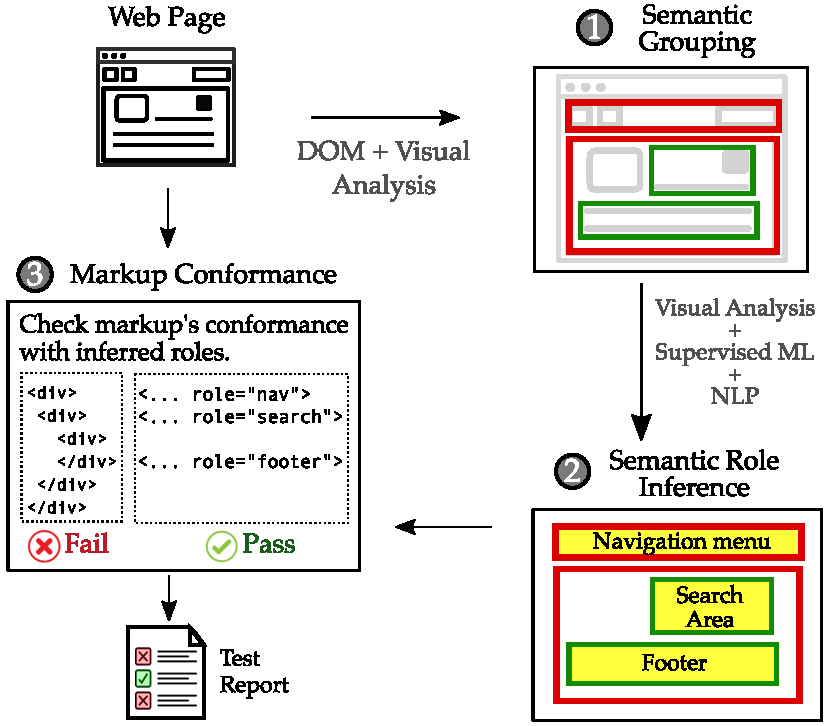
\includegraphics[width=0.7\linewidth]{accessibility_testing/figures/approach/approach.pdf}
    \caption{Overview of the proposed approach.}
    \label{fig:approach}
\end{figure}

\subsection{Visual Objects Identification}
In this first stage,
the goal is to identify objects that 
are perceivable by sighted users, which we refer to as \emph{\vizobjs}. 
For instance, in \Cref{fig:motivating-example}(c), 
each item in the top navigation menu would be a {\vizobj}. 
This step of visual objects identification is the 
foundation of our overall approach, 
since the identification of {\vizobjs} enables checking whether the information
and elements that are perceivable by sighted users 
are also accessible to non-sighted users. 
 

\subsubsection{Objects Extraction}\label{subsec:extraction}

We begin by taking as input the DOM of the page 
after it is loaded and rendered in a browser. We 
then extract from the DOM a set of nodes that 
represent visual content of the page, 
and we refer to each of these as \emph{{\VizObjs}}.
We define three types of {\VizObjs}:
textual, image, and interactive.

\header{Textual Objects}
The extraction of text content is achieved by 
traversing text nodes of the DOM. More specifically:
\begin{align}
    \Theta_{t} \coloneqq \{ E \:\vert\: \nu(E) \land \tau(E) \}
\end{align}
where $\Theta_{t}$ is the set of all {\vizobjs} that represent text in the page,
$E \in DOM$ is a leaf element iterator of the rendered DOM in the browser,
$\nu(E)$ is a heuristic predicate that runs a series of checks
to detect visually perceivable elements (as will be described in \cref{subsub:vizassert}),
and $\tau(E)$ is a predicate that examines whether
there is a text associated with $E$. 
More specifically, it returns
non-empty nodes of DOM type \code{\#TEXT},
which represent string literals. 
An example of extracted textual objects would be the ``Resources'' section in 
\Cref{fig:motivating-example}(c).
We note that the predicate is based on a node type, rather than
an element (i.e., tag) type.
This allows more robust abstraction because the predicate captures any text and does not
make assumptions about how developers choose to place their text.
In other words, regardless of the tag used for text data (e.g., \code{<span>, <div>}),
text would still be stored in nodes of type \code{\#TEXT}, even for custom HTML elements.
This helps in making the approach more robust by reducing assumptions about
tags and how they are used in the page.

\header{Image Objects}
Subsequently, we perform another extraction for image objects.
We define this as follows:
\begin{align}
    \Theta_{m} \coloneqq \{ E \:\vert\: \nu(E) \land \mu(E) \}
\end{align}
where $\Theta_{m}$ is the set of all objects that are present in the page and represent images.
As in the previous case,
the predicate $\mu(E)$ examines whether
there is any relevant image content associated with $E$.
This has two possibilities:
a) nodes of \code{<img>}, \code{<svg>}, and \code{<canvas>} elements, 
and b) non-image nodes with a non-null background image.
An example of extracted image objects would be the bell icon in 
\Cref{fig:motivating-example}(c).
We note that this predicate makes the proposed approach more robust
by eliminating assumptions about how developers markup images. 
If images are contained in standard tags (e.g., \code{<img>}, \code{<svg>}),
then the predicate readily captures them. 
However, we make no assumptions that this is the only way an image can be included.
For this reason, we also capture elements of any type when a non-null background image 
is detected.

\header{Interaction Objects}
Finally, we extract the interaction elements as follows:
\begin{align}
    \Theta_{i} \coloneqq \{ E \:\vert\: \nu(E) \land \eta(E) \}
\end{align}
where $\Theta_{i}$ is the set of all {\vizobjs} that represent form elements 
or similar interactive elements.
These are determined by the predicate $\eta(E)$, which collects
elements such as input fields and drop down menus.
An example of extracted interaction objects would be the Email 
input field in \Cref{fig:motivating-example}(c).


\subsubsection{Visual Assertion}\label{subsub:vizassert}
After the preceding extraction of an initial set of {\vizobjs}, 
this stage proceeds by conducting a visual analysis of the objects. 
This analysis detects if an object is visually perceivable.
We conduct the visual analysis as follows. First, we obtain the box model of 
each object. We use the \emph{computed} box model in order to faithfully 
capture the location as finally rendered on screen. 
Next, we obtain a screenshot of the region defined by the box model. 
We then analyze the screenshot using the Prewitt operator~\cite{nixon2019feature} 
used in computer vision. This operator applies a set of derivatives or 
differentiation operations on the image, and then typically used to detect 
salient visual features in the image (e.g., shapes, textures). 
We therefore use this operator to extract any visual features present in the image,
regardless of the category or form of these features. 
Depending on the presence or absence of visual features in the image, the perceptibility state of the object is determined.
If no visual features are detected, 
the object is deemed to be non-perceivable, and vice versa. 
For example, consider \Cref{fig:motivating-example}(c).
The navigation region in the top, and the 
main content that follows it, are perceivable by sighted users. 
However, web pages also have spacing elements that 
do affect the layout but are not individually perceivable themselves. 
For instance, there can be an element between the navigation bar 
and the ``Resources'' section such that a certain vertical distance is 
maintained below the navigation bar. While such a spacing element certainly 
affects the layout and occupies screen space, 
it does not constitute a {\vizobj} due to it's imperceptibility. 

\subsection{Semantic Grouping} \label{sec:grouping}

After the {\vizobjs} identification is completed,
we proceed by grouping {\vizobjs} into groups representing potential
semantically relevant regions on the page. 
For instance, in \Cref{fig:motivating-example}(c), 
one semantic grouping would be the navigation region 
at the top of the page. 
Another semantic grouping would be the ``Resources'' and ``About Us'' 
sections representing the main content of the page.

The rationale for this step of the approach is as follows. 
We recall that screen readers expect the markup to indicate the 
major semantic regions of a page. 
Accordingly, in order to automatically assert that any visually perceivable semantic 
region has been also expressed in the markup, we first need 
a mechanism by which we can detect the semantic regions in the first place. 
This is what we aim to achieve in this stage. 
Here we are only concerned with creating potential semantic groupings, 
while the next stage (\Cref{sec:role-inf}) attempts to infer what is the semantic 
role (if any) of each potential grouping. 

\hl{
The grouping uses both structural (DOM) information as well as visual analysis. 
The DOM is used to generate a large number of potential seed groupings, 
and the visual analysis performs filtering and further analysis to produce a 
final set of groups.
We adopted this strategy for the following reasons. 
We observed that the DOM can potentially serve as a source of seed groupings. 
This is because of its inherently hierarchical nature that also tend to capture 
the developer's or designer's own intended semantic grouping.
That is, the assumption here is that a set of nodes that has been grouped by a developer 
(i.e., implicitly via DOM hierarchy) is more \emph{potentially} likely to represent some 
semantic value, compared to a random set of nodes. 
We emphasize that the groups only potentially have semantic value, and therefore serve 
only as an initial guess. The final decision 
of whether or not they do actually have a semantic role will be determined at a later stage (i.e., the role inference stage). 
Had we not performed this initial guess, the role inference alone would be practically 
untenable because of the extremely large combinatorial set of possible node combinations. 
}
Subsequently, visual analysis filters these initial seed groups and process 
them to construct semantic groupings. 
Visual analysis is used because, while the DOM may provide seed groupings, 
it does not faithfully represent what the end user is actually observing on the screen. 


\header{Grouping process}
We now describe the mechanism of the grouping process.
First, we obtain one flat non-hierarchical set of all DOM elements. 
For instance, in \Cref{fig:motivating-example}(a), 
this would be all the \code{div} elements in one flat set.
The elements are collected regardless of visibility, due to the complex 
nature of DOM and CSS rendering where non-visible nodes can contain visible children.
For this same reason, the initial set of elements is flat and non-hierarchical, 
because visible children can often be inside non-visible nodes, and therefore relying 
on DOM hierarchy would yield many false positives and negatives. 
Instead, we build the hierarchy by visually analyzing the collected flat set of elements.
We do this by first collecting the computed box model of each element in the set. 
For instance, in \Cref{fig:motivating-example}(a), this would result in a set containing 
the computed box model of each \code{div} element regardless of hierarchy.
Next, we remove box models that are visually located outside the page boundaries, 
since they are not perceivable to sighted users.
For boxes that are only partially outside the page, we trim them to page boundaries. We note that we analyze the page as a whole, 
not only the currently visible portion. 
Subsequently, we filter \emph{equivalent} boxes, which is when a pair of boxes 
visually contain the same set of {\vizobjs}.
We do this by removing the smaller box in terms of visible area in a pair of equivalent boxes. This is because multiple boxes will often 
exist since many DOM elements can share similar visual dimensions 
and regions on screen. 
Next, we filter boxes based on how many {\vizobjs} are visually contained (i.e., located) 
within them. We remove each box that visually contains the entire set of {\vizobjs} on the page. 
For instance, in \Cref{fig:motivating-example}(a), any \code{div} that 
visually contains the entire set of all \code{div}s is removed.
This is because such a set does not represent any semantically useful grouping, 
since the entire set of objects is in one group only. 
Finally, we iterate over the set of {\vizobjs}. 
For each object, we find the largest box that visually contains the object. 
Once this is completed for all {\vizobjs}, the final result is a set of boxes representing 
the potential semantic groupings on the page.


\subsection{Semantic Role Inference}\label{sec:role-inf}
Once semantic grouping is completed, we proceed to infer 
the semantic role of each group. 
This step infers one of the pre-defined landmark roles (\Cref{subsec:aria-roles}). 
An example can be seen in the top navigation bar in \Cref{fig:motivating-example}(c), 
indicating the pre-defined role of \code{navigation}. 
However, not all roles are relevant to our scope of automated 
semantic analysis. For instance, \code{region} is a generic catch-all label that 
does not convey any specific semantic role, and its use is generally discouraged 
and typically not used by screen readers. 
Another example is \code{form}, a label that indicates form regions. 
The label is directly associated with HTML \code{<form>} elements, 
and therefore no semantic analysis or inference is needed for its detection.
Accordingly, we focus our semantic analysis on the more relevant roles of 
\code{main}, \code{navigation}, \code{contentinfo}, and \code{search}, 
which will be described in the following sections. 


\header{Main Role}
The \code{main} ARIA role indicates a region that contains the main output or results 
in a web page. For example, on the search results page of a search engine, 
the region containing the list of retrieved search results would be the main region, 
which is then surrounded by other regions such as the navigation bar or footer.

The process by which we infer the role of a group to be \code{main} is as follows.
First, we compute a score for each detected group in the page. 
The score uses both visual geometrical attributes as well as natural language 
processing (NLP) measurements.
More specifically: 
\begin{align} \label{eqn:score_main}
    \psi_{main}(r) = A(r) \rho(r)
\end{align}
where $r$ is a semantic grouping of the page, $\psi_{main}$ is the score, 
$A(r)$ is the visual geometric area for $r$, and $\rho(r)$ is an NLP 
metric we define to measure linguistic aspects of the contents of $r$. 
More specifically, $\rho(r)$ 
first performs a part-of-speech (POS) tagging, which is a common NLP analysis 
than assigns POS labels (e.g., verb, noun, adjective) to each word. 
$\rho(r)$ then measures the variance of the linguistic POS tag frequencies 
of all textual objects contained in $r$.  
We give an example to clarify the various measured values. 
Consider the rendered page in \Cref{fig:motivating-example}-c. 
$r$ would represent, for instance, the region containing the 
body of the page (e.g., the Resources and About Us sections). 
$A(r)$ would be the geometric area of that region as visible on the screen. 
The rationale is to capture how much would a region occupy the 
visible space for sighted users. 
As for $\rho(r)$, it first collects all textual objects 
(as explained in \cref{subsec:extraction}) within $r$, which would 
collect all text elements such as "Resources", "About Us", as well as the 
paragraphs on the page. For each text object, POS tags are collected,  
and then their frequencies (i.e., count of each tag type) are computed. 
$\rho$ then measures the variance of these POS tag frequencies. 
For instance, a navigation region $r$ that has, say, the textual objects ``Images'', 
``News'', and ``Settings'' has no variance since they all 
have identical POS tags. Contrast this with the main body of text in a page, 
which contains elements such as such as paragraphs, 
section headings, links, and much more. The likelihood of all such content 
to be linguistically monotonous (i.e., all tags are nouns) is practically negligible.
This is why \cref{eqn:score_main} includes the $\rho(r)$ factor.
The $A(r)$ in the equation accounts for the fact that it is unlikely that the main 
region of the page would be the visually smallest area on the page. 
Once the score in \cref{eqn:score_main} is computed for all detected regions, 
we sort the regions by score and select the region with the highest score, 
which is finally reported to be the region having the main role. 
We note that we simply directly multiply the two factors, and do not have any thresholds or weights in order to have a parameter-free and more robust inference. 

\header{Navigation Role}
The \code{navigation} ARIA role indicates a region in a webpage that 
allows users to navigate between various pages or views. 
The process by which we infer the role of a group to be \code{navigation}
is as follows. 
We first compute a score for each group, using the 
following equation:
\begin{align} \label{eqn:score_nav}
    \psi_{nav}(r) = \frac{C(r)}{1 - \rho_h(r)} 
\end{align}
where $r$ is a semantic group of the page, $\psi_{nav}$ is the score, 
and $C(r)$ is a metric that measures the \emph{clickables ratio} 
inside the group $r$. This computes the ratio of {\vizobjs} 
that appear to be clickable to sighted users, which we define as 
any {\vizobj} whose onscreen cursor is a hand or a pointer, 
indicating to sighted users that it can be clicked on. 
Accordingly, a group that has high $C(r)$ is mostly composed 
of objects that a sighted user can click on, which is typically the case 
for navigation regions. 
For example, in \Cref{fig:motivating-example}-c, the yellow 
navigation region at the top contains elements that all appear 
as clickables to sighted users. 
In contrast, a group that does not contain any clickables 
(e.g., only static texts and images) would have a $C(r)$ equal to zero and 
therefore is not a navigation region. 
This can be seen, for instance, in \Cref{fig:motivating-example}-c 
in the body of the page below the navigation bar, where the body 
contains only static text paragraphs or images. 
$\rho_h(r)$ is a measure of the homogeneity of the contents of $r$. 
For semantic groups containing only textual elements, 
$\rho_h(r)$ is the same NLP linguistic 
variance metric we defined in \cref{eqn:score_main}. 
For all other elements, $\rho_h(r)$ represents the dimensional variance 
of the objects in $r$.
Finally, a given group is inferred to have a navigation role 
when $\psi_{nav}$ greater than or equal unity, which was determined experimentally by manually testing this value empirically on a random group of websites.


\header{ContentInfo/Footer Role}
The \code{contentinfo} role (also known as the footer role) indicates 
regions of the page that represent complementary 
content to the parent document. That is, instead of containing the 
main output of the page or the main navigation elements, footer regions 
serve as complementary content or information that comes after 
the main content. 
In a similar fashion to previous roles, we compute a score for each detected 
grouping, using the following equation:
\begin{align} \label{eqn:score_footer}
    \psi_{footer}(r) = \frac{C(r)D(r)}{A(r)} 
\end{align}
where, as in the previous roles, $r$ is a semantic group of the page, 
$\psi_{footer}$ is the score, 
$A(r)$ is the visual pixel count for $r$, $D(r)$ is the visual 
distance from the geometric center of $r$ to the origin of the screen, 
and $C(r)$ is the clickables ratio in $r$ as defined in \cref{eqn:score_nav}.
As can be observed from the equation, the score is mostly concerned 
with the visual geometric aspects of the region, since this ARIA role
is, by definition, spatial in nature since it refers to a specific 
spatial visual placement on the page. 
Accordingly, we compute and sort the score for all groups, 
and select the group with the highest score. If the group is located 
in the lower half of the page, it is reported as a footer. Otherwise no 
footer regions are reported.

\header{Search Role}
The \code{search} ARIA role indicates regions in a page 
that allow users to enter a search query and retrieve items on 
the page or site. To infer this role, we use a combination of 
visual analysis, a supervised machine learning model, as well as 
linguistic (i.e., keyword) techniques.

First, we train a Convolutional Neural Network (CNN) to visually 
recognize search icons. We collected and labeled 
500 data points representing icon images (50\% positive examples) 
and used the Inception CNN architecture~\cite{szegedy2015rethinking}, 
which has been shown to produce very effective classifications for 
computer vision machine learning problems~\cite{szegedy2015rethinking}.
Subsequently, we use this model to find search icons on a page. 
Next, we perform a nearest neighbor search to look for text input 
fields in the spatial vicinity of detected search icons. If a text input field 
is found, we mark the region containing the search icon and the input field 
as having a search semantic role.
Furthermore, we also check for cases where the search input text field 
has no associated search icons. In this scenario, we extract all text 
input fields on the page. We then perform a nearest neighbor search 
to find any visible label texts in the visual spatial vicinity around 
the input field.
We then conduct NLP \emph{stemming} on the label text and find those that 
include key linguistically significant \emph{stem words},
such as ``find'', ``search'', and ``locate.'' 
Any detected group that matches any of the above cases is marked 
as having a search semantic role.

Finally, we note that, due to the non-hierarchical nature of our semantic groupings, 
all inferred roles are agnostic to hierarchies and the proposed approach is therefore able to detect hierarchical combinations of the inferred roles (e.g., a navigation region within a footer region). 



\subsection{Markup Conformance}\label{sec:conformance}
This final stage asserts that the source of the page 
contains markup indicating the presence of the inferred semantic regions
and their semantic roles. 
For instance, in \Cref{fig:motivating-example}(c), the approach so far 
would infer that the group of elements at the top of the page represent 
a coherent semantic grouping, and that their semantic role is navigation.
If the HTML markup corresponding to that area does not contain 
the ARIA landmark role of \code{navigation}, 
then screen readers will not be able to provide this semantic information 
to users, and we recall that this semantic information is 
among the most important and widely used of ARIA roles by users 
with disabilities~\cite{2019users_survey}. 
Therefore, in such cases where the markup does not 
conform to the inferred 
semantic roles, we report an accessibility failure 
and indicate the expected 
semantic markup and where it should have been 
expressed in the page.

The mechanism of checking markup conformance is as follows. 
First, we obtain the semantic groupings and any inferred roles, 
as described in the previous sections. 
For each semantic group, we identify all DOM elements that satisfy two criteria:
1) all {\vizobjs} of the group are located inside the element's box model, and 
2) the element's box model is located inside the group's box model.
This process captures all possible DOM elements that would qualify as 
a root for the region, without including objects from other regions. 
Any of these DOM elements would therefore have to contain markup 
indicating the presence of a region and its role.

We then check whether any element in the set meets both of the following requirements: 
1) the element has a \code{role} attribute whose value matches the inferred semantic role of the group.
2) the element's computed box model visually overlaps the box model of the inferred semantic group.
The rationale for adopting this approach is as follows. 
As we noted in \Cref{sec:grouping}, the complex nature of 
DOM and CSS rendering easily allows cases where non-visible/non-rendered 
nodes can contain visible rendered children. A DOM-based approach 
(e.g., checking containment by XPath) would therefore yield many false positives and negatives. 
Accordingly, we use the visual check above for a more robust analysis. 

If an element satisfying these requirements is found, we log it and move on to the next inferred semantic role and check that it has been correctly expressed in the markup. The process is repeated for all semantic groupings for which a role has been inferred. Any semantic grouping for which no role has been inferred is discarded. A report is finally generated indicating all roles that have been correctly expressed in markup, and all roles that should have been 
in the markup but are missing. We do not assume our approach understands the semantic roles better than what a human being would manually identify, and therefore there no miss-classification is reported if a markup already exists.  

\header{Implementation}
We implemented the proposed approach in a tool called~\toolname  
(short for Accessibility Ray). It is implemented in Java. 
We use Selenium WebDriver to instrument browsers and extract 
DOM information and computed attributes. We use OpenCV~\cite{opencv} 
for computer vision computations, DeepLearning4J~\cite{dl4j} for machine learning operations, and the Stanford CoreNLP library~\cite{stanfordCoreNLP} for linguistic analysis. 
To make the study replicable, we made available online a link to 
our \toolname tool and the anonymized participants' responses~\cite{tool-and-data}.
% !TEX root =  paper.tex
\section{Evaluation}
\label{sec:evaluation}
To evaluate \toolname, we conducted qualitative and quantitative studies  
to answer the following research questions:

\begin{enumerate}[label=\textbf{RQ\arabic*},leftmargin=*]
	\item How accurate is \toolname in inferring semantic groupings and semantic roles?

	\item To what extent can \toolname detect accessibility failures 
    in real-world web pages?
\end{enumerate}

In the following subsections, we discuss the details of the experiments that 
we designed to answer each research question, together with the results.

\subsection{RQ1: Semantic Grouping and Roles Inference}
In this question, the objective is to assess how accurate the semantic grouping and semantic role inference processes are. 
The rationale for evaluating this aspect is that the approach 
first performs the grouping and semantics inference, and then 
uses this inference to test for accessibility. Accordingly, 
we first need to assess the inference process itself. 

We evaluated this question as follows. 
First, we collected 10 random subjects from the Moz 
Top 500~\footnote{https://moz.com/top500} most popular websites. 
Our approach does not have specific requirements for a subject other 
than being able to load it in a browser and access its DOM.  
We then ran the approach on each test subject's URL and obtained 
the output groupings and semantic roles. 
\Cref{fig:output} shows an example of the output. 
Each rectangle represents an inferred grouping, together 
with its semantic role. 
Subsequently, we recruited human evaluators. 
10 evaluators were recruited from the MTurk~\footnote{https://www.mturk.com} 
crowdsourcing platform. The qualifications of participants 
are to be working in the software industry and to have maintained the 
highest level of accuracy on the MTurk platform, which is referred to 
as Masters level.

Subsequently, each human evaluator was presented with the output of \toolname 
for all test subjects, and asked to assess the accuracy of groupings and roles.  
More specifically, we asked them to identify any output groups 
that do not represent a meaningful semantic grouping. This represents 
the \emph{false positives} of groupings, 
while the remainder are \emph{true positives}. 
We also asked them to identify any meaningful semantic groupings on the page 
that were not included in the output. These are the \emph{false negatives}. 
The same process is repeated for the semantic roles.

\subsubsection{Results and Discussion}
\Cref{tbl:rq1} shows the results of evaluating the accuracy 
of semantic grouping and role inference. 
The columns show the precision, recall, and F-1 measure (i.e., the harmonic mean of precision and recall) averaged across evaluators. 
The two groups of columns, labeled ``Grouping inference'' 
and ``Role inference'', 
show the accuracy of the proposed approach in inferring 
semantic groupings and semantic roles, respectively. 
The highlighted cells show the minimum and maximum 
values in each column.

The key outcome of this evaluation is the F-1 measures, 
which are at 87\% and 90\% 
for grouping and role inference, respectively. 
These values indicate a rather effective inference process. 
The lowest precision was 71\%. This often happens due to 
a somewhat unusual DOM structure, where elements in the 
same region were placed at large tree depth separations 
from one another. This resulted in mistakenly grouping a 
number of elements that should have not been grouped.
As for the recall, the lowest performance was at 60\%. 
Such low values often happen in corner cases where 
elements are falsely excluded from groups due to having 
an empty box model stemming from complex nested CSS rules, 
despite being present in the group.  

\begin{figure*}%[t]
	\centering
	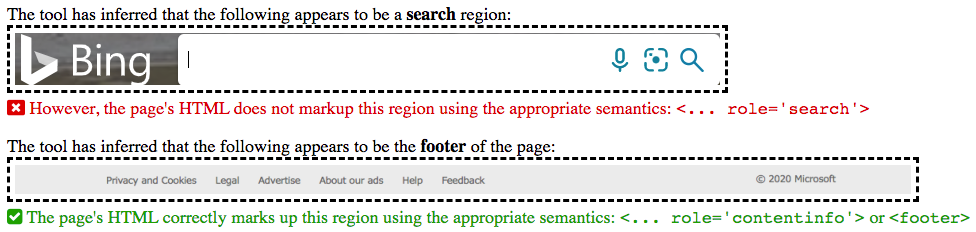
\includegraphics[scale=0.4]{accessibility_testing/figures/output-sample.png}
	\caption{Sample of the generated accessibility report.}
	\label{fig:output}
\end{figure*}


\subsection{RQ2: Accessibility Failures Detection}
While the previous question examined how accurate 
the inferred semantic groupings and roles are, 
this RQ evaluates to what extent the inferred information 
can be used to reliably detect accessibility failures.

\hl{Due to the absence of ground truth data that lists the 
actual failures per subject, 
we evaluate this RQ in two complementary ways: 
1) using a fault injection experiment, 
and 2) evaluating the output on a large number 
of real-world subjects in the wild. 
Each evaluation is independent and separate from the other. 
The rationale for using these two complementary experiments is as follows. 
In the fault injection experiment (as will be explained in \mbox{\cref{subsec:faultinjec}}), 
existing semantic markups (if any) 
are removed. This simulates an accessibility fault since, by definition, 
an accessibility fault is the \emph{absence} of required markup. 
Subsequently, a check is made whether the tool is able to detect the absent markup 
and therefore detect the fault. 
The benefit of this experiment is that it allows automated evaluation 
without a subjective assessment. In other words, it creates a partial 
ground truth data from page developers' own tagging of roles. 
The drawback, however, is that it is only a \emph{lower bound} 
of the actual accuracy, since it says nothing about other possible 
role faults that have not been injected 
(i.e., due to the absence of some roles from the original markup itself). 
For this reason, we supplement the fault injection experiment 
with a manual item-by-item evaluation of the inferred roles  
in order to evaluate all true/false positive and negative results.
We describe each approach in the following subsections. 
We emphasize that the two experiments, fault injection and direct evaluation, 
are separate and independent of each other. That is, whereas the subjects are injected with faults in the first experiment, all subjects are used in their original form 
for the second experiment. }

\begin{table}[t]
    \caption{Precision and recall of grouping and role inference. Highlighted numbers are the minimum and maximum values in each column.}
    \label{tbl:rq1}
  	\centering
    \begin{tabularx}{0.87\textwidth}{lrrrrrr}
                                   & \multicolumn{3}{c}{\textbf{Grouping inference}}                                                                                                  & \multicolumn{3}{c}{\textbf{Role inference}}                                                                                                      \\ 
    \multicolumn{1}{c}{\textbf{Subject}} & \multicolumn{1}{c}{\textbf{Prec.}}               & \multicolumn{1}{c}{\textbf{Recall}}                  & \multicolumn{1}{c}{\textbf{F-1}}               & \multicolumn{1}{c}{\textbf{Prec.}}               & \multicolumn{1}{c}{\textbf{Recall}}                  & \multicolumn{1}{c}{\textbf{F-1}}               \\  \hline
    wikipedia.org                              & 94\%                                        & 89\%                                        & 91\%                                        & 91\%                                        & 91\%                                        & 91\%                                        \\
    google.com                              & 88\%                                        & 85\%                                        & 87\%                                        & 86\%                                        & 81\%                                        & 83\%                                        \\
    amazon.com                              & 92\%                                        & 87\%                                        & 89\%                                        & \cellcolor[HTML]{DCDCDC}{\textbf{83\%}} & \cellcolor[HTML]{DCDCDC}{\textbf{79\%}} & \cellcolor[HTML]{DCDCDC}{\textbf{81\%}} \\
    stackoverflow.com                              & 91\%                                        & 94\%                                        & 92\%                                        & 91\%                                        & 81\%                                        & 86\%                                        \\
    medium.com                              & 96\%                                        & 94\%                                        & \cellcolor[HTML]{DCDCDC}{\textbf{95\%}} & 94\%                                        & \cellcolor[HTML]{DCDCDC}{\textbf{99\%}} & 96\%                                        \\
    khanacademy.org                              & 92\%                                        & \cellcolor[HTML]{DCDCDC}{\textbf{98\%}} & 95\%                                        & 96\%                                        & 89\%                                        & 93\%                                        \\
    imdb.com                              & \cellcolor[HTML]{DCDCDC}{\textbf{71\%}} & 86\%                                        & 78\%                                        & 92\%                                        & 96\%                                        & 94\%                                        \\
    cnn.com                               & \cellcolor[HTML]{DCDCDC}{\textbf{97\%}} & 92\%                                        & 95\%                                        & \cellcolor[HTML]{DCDCDC}{\textbf{97\%}} & 97\%                                        & \cellcolor[HTML]{DCDCDC}{\textbf{97\%}} \\
    rt.com                              & 92\%                                        & \cellcolor[HTML]{DCDCDC}{\textbf{60\%}} & \cellcolor[HTML]{DCDCDC}{\textbf{72\%}} & 94\%                                        & 90\%                                        & 92\%                                        \\
    booking.com                             & 92\%                                        & 73\%                                        & 81\%                                        & 93\%                                        & 89\%                                        & 91\%                                        \\ \hline
    \textbf{Average}               & \textbf{90\%}                               & \textbf{85\%}                               & \textbf{87\%}                               & \textbf{91\%}                               & \textbf{89\%}                               & \textbf{90\%}               \\               
    \end{tabularx}
    \vspace{-0.25cm}

\end{table}

\header{Subjects} We conducted the experiments in this RQ 
on a total of 30 real-world subjects. 
The subjects were collected in two ways. 
The first half of subjects were randomly selected 
from the Moz Top 500 most popular websites as in RQ1. 
The second half of subjects were obtained from Discuvver.com, 
which is a service that returns a random 
website from the internet.

% \begin{table}[]
\begin{table}%[t]
    \caption{Results of detecting fault injections.}
    \label{tbl:rq2}
    \centering
    \begin{tabular}{lrrr}
    \hline
                      & \multicolumn{1}{l}{}                                                    & \multicolumn{2}{c}{\textbf{\# Detected faults}}                                                                                                                                   \\ \cline{3-4} 
    \textbf{Subject}  & \textbf{\begin{tabular}[c]{@{}r@{}}Total \# \\ injections\end{tabular}} & \multicolumn{1}{c}{\textbf{\begin{tabular}[c]{@{}c@{}}proposed\\ approach\end{tabular}}} & \multicolumn{1}{c}{\textbf{\begin{tabular}[c]{@{}c@{}}baseline\\ \end{tabular}}} \\ \hline
    bing.com          & 1                                                                       & 1                                                                                        & 0                                                                                      \\
    youtube.com       & 3                                                                       & 3                                                                                        & 0                                                                                      \\
    google.com        & 4                                                                       & 3                                                                                        & 0                                                                                      \\
    microsoft.com     & 7                                                                       & 5                                                                                        & 0                                                                                      \\
    bbc.com           & 5                                                                       & 3                                                                                        & 0                                                                                      \\
    amazon.com        & 4                                                                       & 3                                                                                        & 0                                                                                      \\
    medium.com        & N/A                                                                     &                                                                                          &                                                                                        \\
    yahoo.com         & 3                                                                       & 1                                                                                        & 0                                                                                      \\
    live.com          & 4                                                                       & 4                                                                                        & 0                                                                                      \\
    paypal.com        & 2                                                                       & 1                                                                                        & 0                                                                                      \\
    blogger.com       & 2                                                                       & 2                                                                                        & 1                                                                                      \\
    netflix.com       & N/A                                                                     &                                                                                          &                                                                                        \\
    stackoverflow.com & 3                                                                       & 3                                                                                        & 0                                                                                      \\
    imdb.com          & 4                                                                       & 3                                                                                        & 0                                                                                      \\
    walmart.com       & 3                                                                       & 2                                                                                        & 0                                                                                      \\ \hline
    fuelly.com        & 1                                                                       & 1                                                                                        & 0                                                                                      \\
    typing.com        & 3                                                                       & 2                                                                                        & 0                                                                                      \\
    iconpacks.net     & 2                                                                       & 2                                                                                        & 0                                                                                      \\
    expatistan.com    & N/A                                                                     &                                                                                          &                                                                                        \\
    memrise.com       & N/A                                                                     &                                                                                          &                                                                                        \\
    retrevo.com       & 3                                                                       & 3                                                                                        & 0                                                                                      \\
    startupstash.com  & 4                                                                       & 3                                                                                        & 0                                                                                      \\
    eatthismuch.com   & 1                                                                       & 0                                                                                        & 0                                                                                      \\
    kdl.org           & 3                                                                       & 2                                                                                        & 0                                                                                      \\
    getpocket.com     & 2                                                                       & 2                                                                                        & 0                                                                                      \\
    retailmenot.com   & 3                                                                       & 3                                                                                        & 0                                                                                      \\
    mailinator.com    & N/A                                                                     &                                                                                          &                                                                                        \\
    myfridgefood.com  & 1                                                                       & 0                                                                                        & 0                                                                                      \\
    joinhoney.com     & 2                                                                       & 2                                                                                        & 0                                                                                      \\
    bannereasy.com    & 1                                                                       & 1                                                                                        & 0                                                                                      \\ \hline
    \textbf{Total}    & 71                                                                      & \textbf{77.5\%}                                                                          & \textbf{1.4\%}                                                                        
    \end{tabular}
    \end{table}




% \begin{table}[t]
%     \caption{Results of detecting fault injections.}
%     \label{tbl:rq2}
%     \centering
%     % \begin{tabular}{0.48\textwidth}{cccc}
%     \begin{threeparttable}
%     \bgroup 
%     \begin{tabularx}{0.43\textwidth}{lrrr}
%     \hline
%     \textbf{Subject} & \begin{tabular}[c]{@{}c@{}}\textbf{Total \#} \\ \textbf{injections}\end{tabular} & \begin{tabular}[c]{@{}c@{}}\textbf{\# Detected}\\ \textbf{faults}\end{tabular} & \begin{tabular}[c]{@{}c@{}}\textbf{\# Undetected}\\ \textbf{faults}\end{tabular} \\ \hline
%     bing.com            & 1        & 1       & 0             \\
%     youtube.com         & 3        & 3       & 0             \\
%     google.com          & 4        & 3       & 1             \\
%     microsoft.com       & 7        & 5       & 2             \\
%     bbc.com             & 5        & 3       & 2             \\
%     amazon.com          & 4        & 3       & 1             \\
%     medium.com          & N/A      &         &               \\   
%     yahoo.com           & 3        & 1       & 2             \\
%     live.com            & 4        & 4       & 0             \\
%     paypal.com          & 2        & 1       & 1             \\
%     blogger.com         & 2        & 2       & 0             \\
%     netflix.com         & N/A      &         &               \\   
%     stackoverflow.com   & 3        & 3       & 0             \\
%     imdb.com            & 4        & 3       & 1             \\
%     walmart.com         & 3        & 2       & 1             \\ \hline 
%     fuelly.com          & 1        & 1       & 0             \\
%     typing.com          & 3        & 2       & 1             \\
%     iconpacks.net       & 2        & 2       & 0             \\
%     expatistan.com      & N/A      &         &               \\    
%     memrise.com         & N/A      &         &               \\  
%     retrevo.com         & 3        & 3       & 0             \\
%     startupstash.com    & 4        & 3       & 1             \\
%     eatthismuch.com     & 1        & 0       & 1             \\
%     kdl.org             & 3        & 2       & 1             \\
%     getpocket.com       & 2        & 2       & 0             \\
%     retailmenot.com     & 3        & 3       & 0             \\
%     mailinator.com      & N/A      &         &               \\      
%     myfridgefood.com    & 1        & 0       & 1             \\
%     joinhoney.com       & 2        & 2       & 0             \\
%     bannereasy          & 1        & 1       & 0             \\ \hline
  
%     \textbf{Total}      & 71       & \textbf{77.5\%}      & \textbf{22.5\%} 
%     % \end{tabular}
%     \end{tabularx}
%     \egroup
%     %% This how it should be used in a cell: \multicolumn{3}{c}{N/A\tnote\textdagger}
%     % \begin{tablenotes}
%     %     \item[\textdagger] Faults could not be injected. Please refer to \cref{subsec:rq2-results} for details.
%     % \end{tablenotes}
% \end{threeparttable}
% \vspace{-0.25cm}
% \end{table}





\subsubsection{Fault injection}\label{subsec:faultinjec}
For the fault injection experiment, we inject a random fault in the markup of each subject, and 
assess if \toolname was able to detect the fault. 
We recall from \Cref{subsec:aria-roles} that a web page 
is deemed inaccessible if there is an \emph{absence} of semantic roles. That is, the developer did not add the necessary semantic markup to the page. Our goal is thus to simulate this behavior by \emph{removing} all existing semantic markups on the page, and therefore create a new page as if the developer had not included the necessary semantic markup, and then check whether our approach can re-detect them. Such markup omission, by definition, is what makes web pages inaccessible, 
and is therefore the only meaningful fault type. 
In other words, any mutation of the markup is effectively a markup omission, 
since the exact expected semantic role would become absent from the markup. Due to the absence of ground truth information, 
the next best unbiased option we have is to assume that if a developer has taken the time to manually identify the role of each region, then we take that to be correct. 
We also note that misspelled attribute values are also effectively markup omissions. 
For instance, suppose that a region should have been marked as a navigation region. 
Whether the \code{navigation} role was completely absent from the markup, 
or was misspelled (i.e., \code{ngavoitn}), both cases are still effectively markup omissions.

We now describe the injection process.
First, we load the subject in an instrumented browser (i.e., via Selenium). 
We then remove all semantic markups on the page 
(i.e., landmark \code{role}s). 
We then apply \toolname on the subject and collect the output.  
If after the fault injection (i.e., removal of \code{role}s) 
\toolname was able to indicate that there should be a semantic \code{role} (per each removed markup), 
we conclude that the injected fault has been caught. 
Otherwise, the fault was not detected. 


\header{Baseline}
In order to have a more thorough evaluation, 
we included a baseline in our experiments. 
We could have just reported the results on their own, but 
adding a baseline offers some perspective on how relatively 
better the approach is. 
However, since there are no existing tools that perform 
semantic checking, 
our baseline consists of a simple random selection process. 
In this process, random regions from the page 
are selected. Next, a random semantic role is 
assigned to each randomly selected region. 
This set of semantic regions and their semantic roles 
is then taken to be the baseline.  

\header{Results and Discussion}\label{subsec:rq2-results}
\Cref{tbl:rq2} shows the results of evaluating the fault 
injection experiment. 
The first column shows the total number of fault injections performed on 
each subject. 
We recall that this first column is not a number we chose; 
it is rather the total number of injections that were \emph{possible}, 
since the faults are removals of existing semantic markup. 
The second column shows the number of injected faults that 
were successfully detected by, whereas the third column shows the 
number of injected faults that the tool has failed to detect. 
The last row sums up the results across all subjects.

The main result of the evaluation is that \toolname has detected, 
on average, around 77.5\% of the injected faults. 
While this performance is relatively good, 
given that this sort of analysis hasn't been automated so far, 
we do note this is only a lower bound of the actual accessibility 
failure detection ability, since it says nothing about other possible 
failures that have not been injected 
(e.g., where the original markup itself did not include certain semantic roles). 

In certain subjects in \Cref{tbl:rq2}, marked with ``N/A'', the fault 
injection process was not possible. 
This was because the subject's markup did not contain any of the landmark semantic roles, 
and therefore it was not possible to remove them and check if our tool 
was able to detect them back. 
Despite some of these subjects being top 100 websites, 
the lack of such markup in the subject is an example that illustrates the need for effective 
and automated accessibility testing.

\subsubsection{Direct output evaluation}
In this step, we manually evaluate the output on a large number 
of real-world subjects in the wild.
First, we loaded each test subject in an instrumented web browser (i.e., via Selenium). 
Page popups or notifications, if any, were closed. 
Next, we applied \toolname on the subject and collected the generated 
output (as shown in \Cref{fig:output}).  
We then categorized each item in the report into one of the following:
\textit{True positive:} 
This represents a true accessibility failure. 
This category holds whenever the tool has reported the absence of 
a correct semantic role that is indeed missing from markup, 
and therefore the reported failure is true.   
\textit{False positive:}
This is a false accessibility failure.
In this case the tool has either reported an incorrect semantic 
role or the role is already in the markup 
but was falsely flagged as missing, and therefore 
the reported failure is false.
\textit{False negative:}
This case is a false accessibility \emph{pass} 
(not failure, as in the two previous cases).
This represents cases where a semantic role should have been included the markup, as determined by manual visual examination of the page, but the approach did not report an accessibility failure. For instance, the page has a search region but the approach did not 
report that role. 
\textit{True negative:}
This corresponds to true accessibility pass.  
This represents cases where a role is actually semantically not present 
on the page, and the tool did not report a failure.
This also corresponds to cases where a semantic role is present in the markup, 
and the tool has reported that the markup is conforming to the inferred semantic role.  

% \caption{Direct evaluation of accessibility failure detection on 30 real-world subjects in the wild.}
% \label{tbl:rq2-run}


% \begin{table}[]

%     \begin{tabular}{lrrrr}
%     \hline
%     \textbf{Subject}  & \textbf{TP}   & \textbf{FP}    & \textbf{TN}   & \textbf{FN}  \\ \hline
%     bing.com          & 4             & 0              & 1             & 0            \\
%     youtube.com       & 0             & 0              & 4             & 0            \\
%     google.com        & 2             & 2              & 3             & 0            \\
%     microsoft.com     & 2             & 1              & 10            & 0            \\
%     bbc.com           & 2             & 2              & 2             & 2            \\
%     amazon.com        & 4             & 0              & 7             & 0            \\
%     medium.com        & 4             & 0              & 1             & 0            \\
%     yahoo.com         & 1             & 0              & 1             & 3            \\
%     live.com          & 2             & 0              & 4             & 0            \\
%     paypal.com        & 3             & 0              & 2             & 0            \\
%     blogger.com       & 1             & 0              & 3             & 1            \\
%     netflix.com       & 2             & 0              & 1             & 1            \\
%     stackoverflow.com & 3             & 0              & 6             & 0            \\
%     imdb.com          & 2             & 2              & 3             & 0            \\
%     walmart.com       & 6             & 0              & 2             & 1            \\ \hline
%     fuelly.com        & 3             & 0              & 2             & 0            \\
%     typing.com        & 2             & 1              & 3             & 2            \\
%     iconpacks.net     & 3             & 0              & 1             & 1            \\
%     expatistan.com    & 2             & 3              & 1             & 0            \\
%     memrise.com       & 4             & 1              & 2             & 0            \\
%     retrevo.com       & 2             & 0              & 3             & 0            \\
%     startupstash.com  & 1             & 0              & 4             & 0            \\
%     eatthismuch.com   & 6             & 0              & 1             & 0            \\
%     kdl.org           & 3             & 1              & 2             & 1            \\
%     getpocket.com     & 2             & 0              & 3             & 0            \\
%     retailmenot.com   & 5             & 0              & 3             & 0            \\
%     mailinator.com    & 2             & 1              & 1             & 0            \\
%     myfridgefood.com  & 2             & 1              & 1             & 1            \\
%     joinhoney.com     & 3             & 0              & 3             & 0            \\
%     bannereasy.com    & 4             & 0              & 2             & 0            \\ \hline
%                                    &               &                &               &              \\
%                                    & \textbf{Acc.} & \textbf{Prec.} & \textbf{Rec.} & \textbf{F-1} \\
%                                    & 85.4\%        & 84.5\%         & 86.3\%        & 85.4\%      
%     \end{tabular}
%     \end{table}

\newcommand{\PreserveBackslash}[1]{\let\temp=\\#1\let\\=\temp}
\newcolumntype{C}[1]{>{\PreserveBackslash\centering}p{#1}}
\newcolumntype{R}[1]{>{\PreserveBackslash\raggedleft}p{#1}}
\newcolumntype{L}[1]{>{\PreserveBackslash\raggedright}p{#1}}


%\begin{table*}[ht]
\begin{sidewaystable}
    \caption{Direct evaluation of accessibility failure detection 
    on 30 real-world subjects. 
    % For comparison, the output of the state-of-the-art (SortSite) is included.
    }
    \label{tbl:rq2-run}
    \centering
    % \begin{tabular}{lrrrrrr}
    % \begin{tabular}{p{1.8cm}p{0.01cm}p{0.01cm}p{0.01cm}p{0.01cm}p{1cm}p{1cm}}
    \begin{tabularx}{0.85\textwidth}{p{2.5cm}R{0.4cm}R{0.4cm}R{0.4cm}R{0.4cm}L{1.4cm}R{1.4cm}R{0.4cm}R{0.4cm}R{0.4cm}R{0.4cm}}
    \hline
                      & \multicolumn{4}{c|}{\textbf{Proposed approach}}                                                                                               & \multicolumn{2}{C{3.2cm}|}{\textbf{SortSite}}                                                                                                                                                                & \multicolumn{4}{c}{\textbf{Baseline}}                                                                                                                               \\
    \textbf{Subject}  & \multicolumn{1}{c}{\textbf{TP}} & \multicolumn{1}{c}{\textbf{FP}} & \multicolumn{1}{c}{\textbf{TN}} & \multicolumn{1}{C{0.3cm}|}{\textbf{FN}} & \multicolumn{1}{C{0.9cm}}{\textbf{\begin{tabular}[c]{@{}c@{}}semantic \\ issues\end{tabular}}} & \multicolumn{1}{C{0.6cm}|}{\textbf{\begin{tabular}[c]{@{}c@{}}syntactic \\ issues\end{tabular}}}            & \multicolumn{1}{c}{\textbf{TP}} & \multicolumn{1}{c}{\textbf{FP}} & \multicolumn{1}{c}{\textbf{TN}}   & \multicolumn{1}{C{0.3cm}}{\textbf{FN}}                                                          \\ \hline
    bing.com          & 4                               & 0                               & 1                               & \multicolumn{1}{R{0.3cm}|}{0}           & 0                                                                                       & \multicolumn{1}{R{0.3cm}|}{11}                                                                                     & 0                               & 3                               & 0                                 & 4                                                                                                                                                                                                \\
    youtube.com       & 0                               & 0                               & 4                               & \multicolumn{1}{R{0.3cm}|}{0}           & 0                                                                                       & \multicolumn{1}{R{0.3cm}|}{10}                                                                                     & 0                               & 2                               & 0                                 & 0                                                                                                                                   \\
    google.com        & 2                               & 2                               & 3                               & \multicolumn{1}{R{0.3cm}|}{0}           & 0                                                                                       & \multicolumn{1}{R{0.3cm}|}{6}                                                                                      & 0                               & 2                               & 0                                 & 2                                                                                                                                              \\
    microsoft.com     & 2                               & 1                               & 10                              & \multicolumn{1}{R{0.3cm}|}{0}           & 0                                                                                       & \multicolumn{1}{R{0.3cm}|}{10}                                                                                     & 0                               & 1                               & 0                                 & 2                                                                                                   \\
    bbc.com           & 2                               & 2                               & 2                               & \multicolumn{1}{R{0.3cm}|}{2}           & 0                                                                                       & \multicolumn{1}{R{0.3cm}|}{3}                                                                                      & 0                               & 4                               & 0                                 & 4                                                              \\
    amazon.com        & 4                               & 0                               & 7                               & \multicolumn{1}{R{0.3cm}|}{0}           & 0                                                                                       & \multicolumn{1}{R{0.3cm}|}{13}                                                                                     & 0                               & 1                               & 0                                 & 4                                                               \\
    medium.com        & 4                               & 0                               & 1                               & \multicolumn{1}{R{0.3cm}|}{0}           & 0                                                                                       & \multicolumn{1}{R{0.3cm}|}{6}                                                                                      & 0                               & 2                               & 0                                 & 4                                                               \\
    yahoo.com         & 1                               & 0                               & 1                               & \multicolumn{1}{R{0.3cm}|}{3}           & 0                                                                                       & \multicolumn{1}{R{0.3cm}|}{9}                                                                                      & 0                               & 3                               & 0                                 & 4                                                               \\
    live.com          & 2                               & 0                               & 4                               & \multicolumn{1}{R{0.3cm}|}{0}           & 0                                                                                       & \multicolumn{1}{R{0.3cm}|}{2}                                                                                      & 0                               & 3                               & 0                                 & 2                                                               \\
    paypal.com        & 3                               & 0                               & 2                               & \multicolumn{1}{R{0.3cm}|}{0}           & 0                                                                                       & \multicolumn{1}{R{0.3cm}|}{13}                                                                                     & 0                               & 2                               & 0                                 & 3                                                               \\
    blogger.com       & 1                               & 0                               & 3                               & \multicolumn{1}{R{0.3cm}|}{1}           & 0                                                                                       & \multicolumn{1}{R{0.3cm}|}{5}                                                                                      & 1                               & 2                               & 0                                 & 2                                                               \\
    netflix.com       & 2                               & 0                               & 1                               & \multicolumn{1}{R{0.3cm}|}{1}           & N/A                                                                                     & \multicolumn{1}{R{0.3cm}|}{N/A}                                                                                    & 0                               & 4                               & 0                                 & 3                                                                                                                                     \\
    stackoverflow.com & 3                               & 0                               & 6                               & \multicolumn{1}{R{0.3cm}|}{0}           & 0                                                                                       & \multicolumn{1}{R{0.3cm}|}{18}                                                                                     & 0                               & 2                               & 0                                 & 3                                                               \\
    imdb.com          & 2                               & 2                               & 3                               & \multicolumn{1}{R{0.3cm}|}{0}           & N/A                                                                                     & \multicolumn{1}{R{0.3cm}|}{N/A}                                                                                    & 0                               & 3                               & 0                                 & 2                                                                                                                                     \\
    walmart.com       & 6                               & 0                               & 2                               & \multicolumn{1}{R{0.3cm}|}{1}           & 0                                                                                       & \multicolumn{1}{R{0.3cm}|}{7}                                                                                      & 0                               & 4                               & 0                                 & 7                                                               \\ \hline
    fuelly.com        & 3                               & 0                               & 2                               & \multicolumn{1}{R{0.3cm}|}{0}           & 0                                                                                       & \multicolumn{1}{R{0.3cm}|}{12}                                                                                     & 0                               & 1                               & 0                                 & 3                                                               \\
    typing.com        & 2                               & 1                               & 3                               & \multicolumn{1}{R{0.3cm}|}{2}           & 0                                                                                       & \multicolumn{1}{R{0.3cm}|}{10}                                                                                     & 0                               & 2                               & 0                                 & 4                                                               \\
    iconpacks.net     & 3                               & 0                               & 1                               & \multicolumn{1}{R{0.3cm}|}{1}           & 0                                                                                       & \multicolumn{1}{R{0.3cm}|}{8}                                                                                      & 0                               & 4                               & 0                                 & 4                                                               \\
    expatistan.com    & 2                               & 3                               & 1                               & \multicolumn{1}{R{0.3cm}|}{0}           & 0                                                                                       & \multicolumn{1}{R{0.3cm}|}{9}                                                                                      & 0                               & 1                               & 0                                 & 2                                                               \\
    memrise.com       & 4                               & 1                               & 2                               & \multicolumn{1}{R{0.3cm}|}{0}           & 0                                                                                       & \multicolumn{1}{R{0.3cm}|}{5}                                                                                      & 0                               & 1                               & 0                                 & 4                                                               \\
    retrevo.com       & 2                               & 0                               & 3                               & \multicolumn{1}{R{0.3cm}|}{0}           & N/A                                                                                     & \multicolumn{1}{R{0.3cm}|}{N/A}                                                                                    & 0                               & 2                               & 0                                 & 2                                                                                                                                     \\
    startupstash.com  & 1                               & 0                               & 4                               & \multicolumn{1}{R{0.3cm}|}{0}           & 0                                                                                       & \multicolumn{1}{R{0.3cm}|}{12}                                                                                     & 0                               & 4                               & 0                                 & 1                                                               \\
    eatthismuch.com   & 6                               & 0                               & 1                               & \multicolumn{1}{R{0.3cm}|}{0}           & 0                                                                                       & \multicolumn{1}{R{0.3cm}|}{15}                                                                                     & 0                               & 3                               & 0                                 & 6                                                               \\
    kdl.org           & 3                               & 1                               & 2                               & \multicolumn{1}{R{0.3cm}|}{1}           & 0                                                                                       & \multicolumn{1}{R{0.3cm}|}{9}                                                                                      & 0                               & 3                               & 0                                 & 4                                                               \\
    getpocket.com     & 2                               & 0                               & 3                               & \multicolumn{1}{R{0.3cm}|}{0}           & 0                                                                                       & \multicolumn{1}{R{0.3cm}|}{7}                                                                                      & 0                               & 1                               & 0                                 & 2                                                               \\
    retailmenot.com   & 5                               & 0                               & 3                               & \multicolumn{1}{R{0.3cm}|}{0}           & 0                                                                                       & \multicolumn{1}{R{0.3cm}|}{2}                                                                                      & 0                               & 2                               & 0                                 & 5                                                               \\
    mailinator.com    & 2                               & 1                               & 1                               & \multicolumn{1}{R{0.3cm}|}{0}           & 0                                                                                       & \multicolumn{1}{R{0.3cm}|}{6}                                                                                      & 0                               & 4                               & 0                                 & 2                                                               \\
    myfridgefood.com  & 2                               & 1                               & 1                               & \multicolumn{1}{R{0.3cm}|}{1}           & 0                                                                                       & \multicolumn{1}{R{0.3cm}|}{8}                                                                                      & 0                               & 2                               & 0                                 & 3                                                               \\
    joinhoney.com     & 3                               & 0                               & 3                               & \multicolumn{1}{R{0.3cm}|}{0}           & 0                                                                                       & \multicolumn{1}{R{0.3cm}|}{7}                                                                                      & 0                               & 3                               & 0                                 & 3                                                               \\
    bannereasy.com    & 4                               & 0                               & 2                               & \multicolumn{1}{R{0.3cm}|}{0}           & 0                                                                                       & \multicolumn{1}{R{0.3cm}|}{5}                                                                                      & 0                               & 1                               & 0                                 & 4                                                               \\ \hline
                    %   & \multicolumn{1}{l}{}            & \multicolumn{1}{l}{}            & \multicolumn{1}{l}{}            & \multicolumn{1}{r|}{}             & \multicolumn{1}{l}{}                                                                    & \multicolumn{1}{l}{}                                                                     \\
                      & \multicolumn{1}{r}{\textbf{Acc.}}                   & \multicolumn{1}{r}{\textbf{Prec.}}                  & \multicolumn{1}{r}{\textbf{Rec.}}                   & \multicolumn{1}{l|}{\textbf{F1}}                     & \multicolumn{1}{r}{}                                                                    & \multicolumn{1}{r|}{}                      & \multicolumn{1}{r}{\textbf{Acc.}}                   & \multicolumn{1}{r}{\textbf{Prec.}}                  & \multicolumn{1}{r}{\textbf{Rec.}}                   & \multicolumn{1}{l}{\textbf{F1}}                                                                                                                                                                                                             \\
                      & 85.4\%                          & 84.5\%                          & 86.3\%                          & \multicolumn{1}{r|}{85.4\%}                    & \multicolumn{1}{r}{}                                                                    & \multicolumn{1}{r|}{}                                                                                        & 0.6\%                          & 1.3\%                          & 1.0\%                          & \multicolumn{1}{r}{1.2\%}                                           
    % \end{tabular}
\end{tabularx}
    \vspace{-0.25cm}
%    \end{table*}
\end{sidewaystable}


\header{Results and Discussion}\label{subsec:run-results}
\Cref{tbl:rq2-run} shows the results of the evaluation. 
Each row lists the subject, the true positive/negative and 
the false positive/negative for the subject. 
The last row shows the accuracy, precision, 
recall, and the F-1 measure. 

The values of the accuracy, precision, and recall 
are between 84\% and 86\%, indicating a relatively good 
performance. The true positive column represents the 
true accessibility failures that are indeed present in the subjects. 
This certainly does not cover all possible accessibility failures, 
but rather the subset of accessibility issues that we focus on in this 
work (i.e., the semantic roles).
The true negative column can be thought of as the number of cases 
where the markup of the subject is ``in agreement'' 
with the tool's output.  
In the median, two true accessibility failures were detected per subject, 
and two inferred semantic roles per subject were in agreement with what has been 
expressed in the markup. 
For the second half of subjects in \Cref{tbl:rq2-run} (i.e., the random sites), 
60\% have used semantic roles. In contrast, for the subset of top websites 
(i.e., the first half of subjects), 
74\% have used semantic roles.
40\% of the random websites did not use any semantic roles, compared 
to 26\% of the top websites.    
This observation is expected since top sites are more likely 
to have more resources to create better products. 
The average execution runtime was 17 seconds.

We then investigated the reasons behind the false positives and negatives. 
One common reason is erroneous inference of navigation roles. 
This occurred, for instance, for a region that consisted of weather forecast 
for the next few days. From the perspective of our inference procedure, 
this looked like a navigation area since it had a group of links that were 
coherent in content and presentation (in the sense described in \Cref{sec:role-inf}).
Accordingly, it was falsely indicated as a navigation (i.e., a false positive), and therefore resulted 
in a false accessibility failure. Another reason involves missing footer roles 
that should have been reported. This occurred, for instance, 
for a region that was not recognized by the semantic grouping stage, and therefore 
no role was able to be inferred for it.

For comparison, \Cref{tbl:rq2-run} also includes an evaluation 
of SortSite\footnote{https://www.powermapper.com/products/sortsite/}, 
which is the best performing state-of-the-art 
accessibility testing tool~\cite{ukgov:audit:2018}. 
As mentioned in the introduction, SortSite and other state-of-the-art tools 
only perform syntactic checks and is therefore 
unable to detect the semantic issues 
that are the focus of this work. Accordingly, we run 
an evaluation that verifies this empirically. 
Each subject is fed to SortSite, and the output report is saved. 
Each reported failure is then 
categorized as either a syntactic issue or a semantic issue. 
We recall that, as discussed in \Cref{subsec:syncheckers}, 
a syntactic issue is any failure that only checks the syntax 
of the HTML. Examples include checks like (``each \code{a} 
element must contain non-empty text''), or (``\code{input} must not 
appear as a descendant of \code{a}''). 
These are direct checks that are only concerned with syntax. 
Compare this, for instance, with the reported failure shown in \Cref{fig:output}. 
Here, the failure is \emph{semantic} in nature. That is, the failure 
is not an application of some syntactic rule. Rather, 
the failure is reported because the markup does not conform to how the 
page \emph{is semantically perceived} from a visual perspective, not 
because it didn't conform to a predetermined syntactic rule. 

From \Cref{tbl:rq2-run}, we observe that SortSite was able to 
find many syntactic issues 
(rows with N/A are cases were the tool was unable to load the subject). 
However, it did not detect any of the semantic issues. 
This is expected, as the rationale for this work was the observation 
that the state-of-the-art only conduct syntactic checks, which cannot 
detect the more important and widely used semantic information. 

\subsubsection{Future work}
In this work, we focused on an important subset of accessibility requirements, 
which are the semantic roles as discussed in \ref{header:targeted-roles}. 
Therefore, as expected, our approach 
can not cover all possible accessibility requirements. 
This leaves open a number of avenues 
for future work to address other accessibility requirements, each of which would require 
a novel technique to address. 
The variations in the semantics of various accessibility requirements and the lack of approaches 
to address them, mainly due to the difficulty of performing high-level semantic analysis, 
presents a rich and fertile ground to conduct research, which has received little attention 
from the software engineering research community as discussed in the introduction. 
For future work, we believe it will be a fruitful and interesting pursuit for the research 
community to explore some of these other accessibility requirements.

\subsubsection{Threats to validity}
We chose test subjects (i.e., web sites) randomly from the Internet
with the mentioned criteria in \Cref{sec:evaluation},
to avoid any selection bias.
Plus, the participants were selected to be highly qualified 
evaluators at the crowdsourcing platform, 
mitigating the threats to the internal validity of the study.
The subjects are diverse and complex enough
to be representative of real-world scenarios,
mitigating the external validity of the study by making the results generalizable.
To make the study replicable, we made available online a link to 
our \toolname tool and the anonymized participants' responses~\cite{tool-and-data}.

\section{Related Work}

\header{Accessibility attribute checkers}
Existing approaches related to accessibility testing focus on checking 
syntactical attributes. 
Eler et al.~\cite{eler2018automated} and Patil et al.~\cite{patil2016enhanced} 
check for missing or wrong UI attributes in Android apps, 
such as missing alternative 
text attributes in images, or color attribute values 
below a certain threshold. 
Similar checks are also used in other tools such as 
Google's Accessibility Scanner~\cite{goog_scanner}, 
WAVE~\cite{wave_tool}, and ASLint~\cite{aslint_tool}.
The aforementioned works focus on syntactic checks, 
as opposed to the proposed approach in this work which 
checks for high-level aspects such as page structure and semantic 
landmarks, which are the most important ARIA roles that users 
with disabilities rely on~\cite{2019users_survey}. 

\header{Accessibility guidelines}
The majority of existing work lies within the 
accessibility research community 
rather than software engineering.
This research area involves studying certain categories of websites 
(e.g., airline websites~\cite{agrawal2019evaluating,dominguez2018website}, 
education portals~\cite{kimmons2017open}, 
other categories~\cite{bhagat2019evaluation,ross2018examining,snider2020accessibility,serra2015accessibility}) or 
certain platforms (e.g., Android~\cite{alshayban2020accessibility,park2014toward,yan2019current}), 
and then focusing on \emph{manually observing} how non-sighted users 
would use those apps or websites in order to 
identify any patterns or trends in accessibility, with the 
purpose of publishing improved accessibility guidelines. 
Another line of work focuses on researching software development 
\emph{best practices} and how do they impact the accessibility 
of the end product. 
For instance, Sanchez et al.~\cite{sanchez2017method} and 
Bai et al.~\cite{bai2018categorization, bai2019methods} 
examine development practices in 
agile teams working on accessible software, 
with the goal of proposing a guideline 
for better agile practices. 
Krainz et al.~\cite{krainz2018can} investigates 
the impact of a model-driven approach to development 
on the accessibility of the created product.
None of the aforementioned works, however, is concerned 
with developing an automated approach to test accessibility.
Instead, their focus is researching best practices or guidelines for
developers and designers.

\header{Visual analysis}
There exist a few techniques that analyze web applications from a visual perspective.
Choudhary et al.~\cite{choudhary2012crosscheck} propose an approach that detects 
cross-browser compatibility by examining visual differences between the same app 
running in multiple browsers.
Burg et al.~\cite{burg2015explaining} present a tool that helps developers 
understand the behavior of front-end apps. It allows developers to specify 
the element they are interested in, then tracks that element for any 
visual changes to understand code behavior. 
Bajammal et al.~\cite{bajammal2018generating} propose an approach to generate reusable web 
components by analyzing design mockups.
In contrast to our work, none of these works are related to accessibility. 




\section{Conclusion}

Software accessibility is the notion of building software that 
is usable by users with disabilities. Traditionally, software 
accessibility has often been an afterthought or a nice to have 
optional feature. However, software accessibility is increasingly 
becoming a legal requirement that must be satisfied. 
While some tools exist to perform basic forms of accessibility checks, 
they focus on syntactic checks, as opposed to checking the more critical 
high level semantic accessibility features that users with disabilities 
rely on. 
In this chapter, we proposed an approach that automates web accessibility 
testing from a semantic perspective. It analyzes web pages using a combination 
of visual analysis, supervised machine learning, and natural language 
processing, and infers the semantic groupings present in the page 
and their semantic roles. 
It then asserts whether the page's markup matches the inferred semantics. 
We evaluated our approach on 30 real-world websites and assessed the accuracy 
of semantic inference as well as its ability to detect accessibility failures. 
The results show, on average, an F-measure of 87\% for 
inferring semantic groupings, and an accessibility failures detection accuracy 
of 85\%.



%\bibliography{IEEEabrv,bibliography}

\chapter{Web form accessibility labeling}
\label{chp:accessibility_repair}

%% !TEX root =  paper.tex

% \usepackage{cite}
% \usepackage{amsmath,amssymb,amsfonts}
% \usepackage{algorithmic}
% \usepackage{graphicx}
% \usepackage{subcaption}
% \usepackage{textcomp}
% \usepackage{xcolor}
% \usepackage{multicol} % \columnbreak
% \usepackage{balance}
% \usepackage{enumitem}    
%\usepackage[table]{xcolor}
%\usepackage{nohyperref}

\usepackage{xcolor}

\usepackage{tabularx} 
\usepackage{collcell}

% \usepackage[usenames,dvipsnames,svgnames,table,xcdraw]{xcolor}
% \usepackage[usenames,dvipsnames,svgnames]{xcolor}
% \usepackage{pgfplots}
% \pgfplotsset{compat=1.10}


\usepackage{booktabs}
\usepackage[caption=false,font=normalsize,labelfont=sf,textfont=sf]{subfig}
%\usepackage{cite}
% \usepackage{hyperref}
\usepackage{array}
\usepackage{threeparttable}
\usepackage{enumitem}    
\usepackage[greek,english]{babel}
\usepackage{ifthen}
\usepackage{xspace}
\usepackage{fancybox}
\usepackage{marginnote}
\usepackage{tcolorbox}
\usepackage{multirow}
\usepackage{mathtools}
\usepackage{algpseudocode, algorithm, algorithmicx}
\usepackage{color}
\usepackage{soul}
\usepackage{graphicx}
\usepackage{amsmath}
\usepackage{tikz}
\usepackage{cleveref}
\usepackage{hhline}
\usepackage{balance}

\usepackage{listings}
\usepackage{parcolumns}
\usepackage{cleveref}

\usepackage{array}

\usepackage{adjustbox}
\usepackage{flushend}
\usepackage[switch]{lineno}
\definecolor{light-gray}{gray}{0.95}
\newcommand{\code}[1]{\colorbox{light-gray}{\fontsize{9pt}{10pt}\texttt{#1}}}

\definecolor{circled-color}{gray}{0.15}
\newcommand*\circled[1]{\tikz[inner sep=.1ex,baseline=-.75ex] \node[circle,draw,color=white,fill=circled-color] {#1};}


\def\BibTeX{{\rm B\kern-.05em{\sc i\kern-.025em b}\kern-.08em
    T\kern-.1667em\lower.7ex\hbox{E}\kern-.125emX}}
\newboolean{showcomments}
\setboolean{showcomments}{true}
\hypersetup{draft,bookmarks=false}

\ifthenelse{\boolean{showcomments}}
{
	\definecolor{myyellow}{RGB}{255, 228, 26}
	\definecolor{myblue}{RGB}{50, 50, 220}
	\newcommand{\nb}[2]{
		{\sf
			\fcolorbox{myyellow}{yellow}{\scriptsize\textbf{#1}}%
			$\blacktriangleright$%
			{\color{myblue}\fontsize{7pt}{8pt}\selectfont\textbf{#2}}%
		}%
	}
}
{
	\newcommand{\nb}[2]{}
}


\newcommand{\Mo}[1]{\nb{Mo}{#1}}
\newcommand{\Ali}[1]{\nb{Ali}{#1}}


\usepackage{color}


\definecolor{editorGray}{rgb}{0.95, 0.95, 0.95}
\definecolor{editorOcher}{rgb}{1, 0.5, 0} % #FF7F00 -> rgb(239, 169, 0)
\definecolor{editorGreen}{rgb}{0, 0.5, 0} % #007C00 -> rgb(0, 124, 0)

\lstdefinelanguage{JavaScript}{
  morekeywords={typeof, new, true, false, catch, function, return, null, catch, switch, var, if, in, while, do, else, case, break},
  morecomment=[s]{/*}{*/},
  morecomment=[l]//,
  morestring=[b]",
  morestring=[b]'
}
\lstdefinelanguage{HTML5}{
        language=html,
        sensitive=true, 
        alsoletter={<>=-},
        otherkeywords={
        % HTML tags
        <html>, <head>, <form>, </form>, <div>, </div>, <p>, </p>, 
        <span>, </span>, <input, <textarea, </textarea>, <select, </select>, 
        <option>, </option>, <title>, </title>, <meta, />, </head>, <body>,
        <canvas, \/canvas>, <script>, </script>, </body>, </html>, <!, html>, <section>, </section>
        },  
        ndkeywords={
        % General
        =,
        % HTML attributes
        charset=, id=, width=, height=, type=, value=, checked
        % CSS properties
        border:, transform:, -moz-transform:, transition-duration:, transition-property:, transition-timing-function:
        },  
        morecomment=[s]{<!--}{-->},
        tag=[s]
}

\lstdefinelanguage{CSS}{
  morekeywords={background,color,display,justify,content,font,weight,border,size,padding},
  morestring=[s]{:}{;},
  sensitive,
  morecomment=[s]{/*}{*/}
}
\newcommand{\todo}[1]{\textcolor{magenta}{\nb{TODO:}{#1}}}
\newcommand{\header}[1]{\par\smallskip\noindent\textbf{#1.}}
\newcommand{\toolname}{\textsc{AxeForm}\xspace}
\newcommand{\html}{\textsc{HTML}\xspace}
\newcommand{\css}{\textsc{CSS}\xspace}
\newcommand{\javascript}{\textsc{JavaScript}\xspace}
\lstset{%
    % Basic design
    backgroundcolor=\color{editorGray},
    basicstyle={\linespread{1.0}\scriptsize\ttfamily},   
    frame=l,
    % Line numbers
    xleftmargin={0.75cm},
    numbers=left,
    stepnumber=1,
    firstnumber=1,
    numberfirstline=true,
    % Code design   
    keywordstyle=\color{blue}\bfseries,
    commentstyle=\color{darkgray}\ttfamily,
    ndkeywordstyle=\color{editorGreen}\bfseries,
    stringstyle=\color{editorOcher},
    % Code
    language=HTML5,
    alsolanguage=JavaScript,
    alsodigit={.:;},
    tabsize=2,
    showtabs=false,
    showspaces=false,
    showstringspaces=false,
    extendedchars=true,
    breaklines=true,        
    % Support for German umlauts
    literate=%
    {Ö}{{\"O}}1
    {Ä}{{\"A}}1
    {Ü}{{\"U}}1
    {ß}{{\ss}}1
    {ü}{{\"u}}1
    {ä}{{\"a}}1
    {ö}{{\"o}}1
}




		
%\begin{abstract}

Filling web forms is a common online activity. 
Web forms are made accessible to users with disabilities 
by conveying their content through specific DOM labeling 
markups. The absence of these markups is one of the most 
common accessibility errors. However, there is currently 
little to no work in terms of having an automated analysis 
process that allows inferring the labeling markups in order 
to automatically make forms accessible for users with disabilities. 
In this paper, we propose a web form analysis approach that 
infers labels by first constructing different types of 
visual cues from a form, then optimizing the combination of 
various cues and form fields, and finally augmenting the DOM 
to incorporate the required labeling markup. We evaluate 
our approach on real-world subjects and assess the accuracy 
of labeling inference, the safety of the DOM augmentation, 
as well as the labeling performance. The results show an 
average F1-measure of 88.4\% for label inference, and an 
average run-time of around 1.6 seconds.

\end{abstract}

\keywords{web forms, accessibility errors, 
accessibility repair, visual analysis}

%\maketitle
% !TEX root =  paper.tex
\section{Introduction}

Filling web forms is a common activity while browsing the web. 
The accessibility of web forms for users with disabilities 
requires the presence of markup that explicitly defines the form's 
structure and content. The markups, which are HTML attributes that are 
pre-defined by the World Wide Web Consortium (W3C)~\cite{ARIA}, provide 
a standardized and programmatic non-visual representation of the form, 
thereby enabling non-sighted users to access the form. 
In this chapter, we focus on markups of \emph{web form labeling}, 
which is the explicit declaration of the labels for all fields present 
in a form. The absence of this form labeling markup is one of the 
most common web accessibility errors~\cite{webaim:1mil}.
\renewcommand{\toolname}{\textsc{AxeForm}\xspace}
 
\hl{There is currently little to no proposed software analysis 
approaches that infer web form labeling. Having such a process 
would help in addressing a number of issues. First, the lack of web 
accessibility impacts millions of people around the world~\mbox{\cite{stats:accessibility_population:US, stats:accessibility_population:EU}}. 
Such users would benefit from a software analysis approach that 
automatically makes web forms more accessible, especially because 
missing labeling markup is one of the most common accessibility 
errors~\mbox{\cite{webaim:1mil}}.} For developers, it has been shown
~\cite{vendome2019can,harper2012web} that the general adoption 
of accessibility in some software projects has been low due to 
other competing and pressing development and business requirements, 
and therefore having an analysis approach that can fix form 
labeling errors would be helpful in automating and reducing workload. 
\hl{Furthermore, accessibility is increasingly becoming a legal 
requirement for software products~\mbox{\cite{stats:accessibility_lawsuits:US_1, stats:accessibility_lawsuits:US_2}}, and therefore research towards 
automating some of the accessibility analysis would reduce the workload on developers and their companies. } 
Accordingly, for the aforementioned reasons, proposing an 
automated form label analysis approach would be an important 
addition to the software analysis literature. 

Existing approaches perform testing of accessibility markups, but do not 
conduct labeling inferences to repair the form and make it accessible. 
Eler et al.~\cite{eler2018automated} check for missing attribute fields or 
incorrect attribute values related to accessibility of web pages in general, 
an approach that is also used in a few patents~\cite{sap2019accessibility, breeds2014software}.
A number of tools have also been developed to check for and improve various subsets 
of markup~\cite{yesilada2019web, asakawa2019transcoding}, 
but do not infer or repair missing DOM labeling markups. 
The bulk of existing literature focuses on non-software engineering topics such as 
evaluating best experimental practices for conducting empirical 
accessibility evaluations~\cite{braga2014applying,bayer2006accessibility,
alshayban2020accessibility, snider2020accessibility, bhagat2019evaluation}
None of these works propose any software analysis techniques for form 
labeling. Accordingly, the existing standard practice for repairing 
software accessibility errors has remained a manual laborious process
~\cite{yesilada2019web, acosta2018toward, bai2016evaluation,
brajnik2008comparative,abou2008web}. 

In this chapter, we propose a web form analysis approach that automates the repair of 
form labeling markup. 
The approach is based on visually analyzing the content and structure of a 
web form, and then augmenting the inferred labels into the Document Object Model (DOM). 
This analysis first converts the form into a set of abstract elements 
in order to streamline subsequent analysis.  
Next, a set of cues consisting of visual prominence and layout cues are 
constructed from these elements. 
Subsequently, the labeling process is achieved by solving a set of 
objective functions and constraints in order to reach the final labeling 
associations. Finally, these associations are converted into standard labeling markup in order to make the form labels accessible. 

%\begin{figure*}[t]
    %\centering
    %\begin{minipage}[t]{.44\textwidth}
  %% \begin{figure}[b]
    %\centering
    %\includegraphics[width=0.88\columnwidth,height=5.0cm]{figures/population-plot}
    %% \hspace{1cm}
    %\caption{Number of people with software-related disabilities (e.g., vision, hand control, cognitive, or hearing) in the United States
    %and the European Union. 
    %% To put the numbers in perspective, the number of people with impairments is
    %% comparable to the population of entire countries. 
    %(Data compiled from: \cite{stats:accessibility_population:US, stats:accessibility_population:EU})}
    %\label{fig:population-plot}
  %% \end{figure}
  %\end{minipage}
  %\hspace{1cm}
  %\begin{minipage}[t]{.44\textwidth}
  %% \hfill
  %% \begin{figure}[b]
    %\centering
    %\includegraphics[width=0.91\columnwidth,height=5.0cm]{figures/lawsuits-plot}
    %\caption{Number of software accessibility lawsuits filed in US federal courts per year. The number of lawsuits increased by around 3800\% over the four-year period 2015-2018. (Data compiled from: \cite{stats:accessibility_lawsuits:US_1, stats:accessibility_lawsuits:US_2})}
    %\label{fig:lawsuits-plot}
  %% \end{figure}
  %\end{minipage}
  %\end{figure*}

\begin{figure}
    \noindent
	\begin{minipage}[c]{.97\columnwidth}
        \centering
        \begin{lstlisting}[language={HTML5},frame=ltbr,aboveskip=1.1em,basicstyle={\linespread{1.0}\footnotesize\ttfamily},]
<form>
<section>
 <div><p>Name</p></div>
 <div><p>Business Email</p><span>free providers not accepted</span></div>
</section>
<input type="text" id="vr_9481">
<textarea id="bx_3978"></textarea>
<input type="text" id="vr_6588">
<div><p>Message</p></div>
<section>
 <div><p>Do you have an open ticket?</p></div>
 <div><p>How often should we email you?</p></div>
 <span>Yes</span><span>No</span>
</section>
<input type="radio" value="Y" id="op_y">
<input type="radio" value="N" id="op_n" checked>
<select id="frq"><option>daily</option>
 <option>weekly</option><option>monthly</option>
</select>
</form>
        \end{lstlisting}
    (a) Sample of the HTML markup
    \end{minipage} \hfill
	\begin{minipage}[c]{\columnwidth}
        \centering
        \fbox{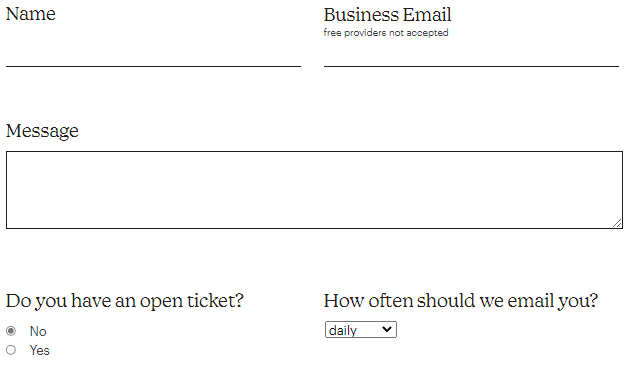
\includegraphics[width=\linewidth]{accessibility_repair/figures/motivating-example/rendered.png}}
        (b) Rendered form
    \end{minipage}
%	\begin{minipage}[c]{.98\columnwidth}
%	\centering \ \\
%	(a) Sample of the HTML markup
%	\end{minipage}
%	\begin{minipage}[c]{.98\columnwidth}
%	\centering \ \\
%	(b) Rendered form
%	\end{minipage}
	\ \\ \caption{An example of an inaccessible web form.}
    \label{fig:motivating-example}
  \end{figure}

This chapter makes the following main contributions:
\begin{itemize}
    \item A novel web form analysis approach for automatically inferring form 
    labeling markup, which is the first to address this issue, to the best of our knowledge.
    \item A technique that is based on a combination of visual cues and 
	optimization formulation to repair the DOM of a web form in order to have accessible labels. 
    \item A qualitative and quantitative evaluation in terms of accuracy, safety, and performance. 
The results show an average F-measure of 88.4\% for labeling accuracy, and an average run-time of around 1.6 seconds.
	\item An implementation of our approach, available in a tool called \toolname~\cite{tool-and-data}.
\end{itemize}


% !TEX root =  paper.tex

\section{Background and Motivating Example} \label{sec:motivation}
\Cref{fig:motivating-example} shows an example of
an inaccessible web form. 
By looking at the rendered form in \Cref{fig:motivating-example}b,
a sighted user can understand 
the structure and content of the web form and navigate their way through it.
For instance, the user would recognize 
that they can write down their name, email, and indicate if they 
would like to receive daily emails. Most importantly, the user recognizes 
which form fields are associated with the name or the email, for instance. 
The collection of information we just described is referred to as form labeling. 
It indicates what fields are present on the form and specifies the textual 
label that describes what each field represents. 

While this understanding of form content and labeling happens naturally when 
sighted users look at the form, that is not the case for visually impaired 
(i.e., non-sighted) users due to the absence of visual perception. 
In \emph{inaccessible} forms, such as the one in \Cref{fig:motivating-example}, 
the labeling is communicated exclusively through visual design. 
This is because the HTML markup in \Cref{fig:motivating-example}a 
is just a collection of \code{<div>}s, \code{<p>}s, and \code{<input>}s 
that do not communicate any labeling associations to indicate what the various 
elements represent. For instance, in \Cref{fig:motivating-example}a, there is no 
piece of markup indicating what the \code{<textarea>} represents or means. 
That is, there is no markup that describes to a non-sighted user 
what information they are supposed to provide for that form field. 
The form is therefore unusable in this case. 
In contrast, sighted users understand 
that the \code{<textarea>} is where they should write down their message, 
or that the first text input is where they should provide their name. 
They understood this from the visual design and layout 
of the form. This implicit visual communication is natural for sighted 
developers and users, but is unavailable for users who can 
not have access to visual information due to disabilities. 
Accordingly, the web form is deemed inaccessible since its markup does 
not specify the labels of the form elements. 


%\subsection{Accessible Rich Internet Applications}\label{subsec:aria-roles}
%Non-sighted users rely on screen readers  
%to parse a web page for them since they can not directly 
%perceive the page. 
%Screen readers are tools that speak out the various information, 
%forms, and labels present on the page, and the non-sighted 
%user would then select one of the 
%options they heard. 
%While a standard web browser simply renders the page as is and leaves 
%it to the end user (i.e., a sighted user) to visually understand what the 
%various elements mean or represent, 
%screen readers require that the page markup explicitly 
%indicates any semantic information (e.g., form labeling)  
%in order to determine what information to convey audibly to the users. 
%
%The standard markup that is used by screen readers during their processing 
%of pages is the World Wide Web Consortium's (W3C) \emph{Accessible Rich 
%Internet Applications} (ARIA)~\cite{ARIA} standard. 
%The ARIA standard specifies a set of markup attributes that 
%should be included in the page's HTML to make it accessible to screen readers. 
%Accordingly, when web developers incorporate these markups into their pages, 
%the result is an accessible app that non-sighted users can use through their 
%screen readers. 
%
%\subsection{Syntax checks}\label{subsec:syncheckers}
%Existing accessibility testing tools~\cite{yesilada2019web,ukgov:audit:2018} 
%are based on syntactic checking. 
%They check the HTML against certain syntax rules. 
%For instance, one common check is to assert that every \code{img} element 
%has an \code{alt} text attribute for textual image descriptions. 
%Another check asserts that \code{input} elements must not 
%be descendant of \code{a}.
%Another example is checking that every \code{ul} list 
%element has a non-empty list item \code{li} child.  
%In general, all syntax checks follow the same template: 
%if certain syntax A is present, 
%assert that syntax B is true. 
%%Established accessibility guidelines (e.g., Web Content Accessibility Guidelines -- WCAG~\cite{WCAG}) 
%%includes a number of such syntax rules as well as other guidelines. 
% 
%While syntax checks can be useful and simple 
%assertions, and are easy to automate, 
%syntax checks are not capable of addressing the more important, 
%and more challenging, analysis that is 
%required to infer and repair form labeling. 
%To illustrate this, we revisit \Cref{fig:motivating-example}(b), 
%where we can visually see that there is a text box form field 
%whose label is `Message`. 
%We perceived this labeling association by visually looking at 
%the rendered form in (b).  
%However, when we look at the markup in (a) we do not find that 
%labeling expressed in the markup, 
%and therefore conclude that the form is inaccessible.  
%We now pause to reflect and observe that there is no possible 
%syntactic check 
%that can automate the conclusion we just reached. 
%Checking that an attribute is missing is simple and readily 
%automatable, but determining 
%what values it should contain is difficult. 
%The steps that we just walked through requires 
%our own visual perception as sighted developers or users in 
%order to reach the conclusion 
%that there is a mismatch between the visually perceived labeling 
%of the from, and the form's markup. 
%

% !TEX root =  paper.tex
\section{Approach}

The objective of this chapter is to propose a web form analysis approach 
to automatically create the required DOM markup for accessibility labels. 
The challenges involved in formulating such an approach are as follows. 
First, web pages and forms can have many possible designs and patterns. 
Designing an approach that addresses every potential case is not tractable. 
Therefore, the goal is to first establish an approach that works for many forms while 
remaining generic and robust. This is an important first step since the problem 
of inferring labeling markup has not been addressed before, so the first stage is 
to establish a technique that can be demonstrated to work for many forms, 
after which other corner cases can be addressed by permutations and adjustments 
in subsequent publications. The second challenge is the absence of prior blueprint 
or similar work that can serve as a starting point to formulate the approach. 
It is therefore not readily evident what assumptions are safe to make or what 
sort of analysis steps or general analytic approaches should be utilized to 
address the problem. Accordingly, the approach will be mainly heuristic in 
nature, and its efficacy will ultimately be assessed in the evaluation.  

The overall steps of our approach are as follows. We adopt a strategy of visually 
analyzing the web form to infer labeling associations of form elements, 
and then repairing the DOM such that its markup reflects 
the inferred labels in order to make the form accessible.
The approach begins by loading the web page in an instrumented web browser 
(e.g., via Selenium). 
Next, any forms on the page are then abstracted in preparation for further 
analysis. 
Subsequently, a set of visual cues are constructed from each form. 
These visual cues are then used in the next stage, which is the optimization 
formulation. In this stage, we cast the labeling process as an optimization 
problem, where the minimization and maximization of certain combinations 
of visual cues yield the final form labels. 
Finally, the inferred labels are transformed into standard ARIA accessibility 
attributes and augmented into the DOM of the web page. 

\subsection{Form Abstraction} \label{sec:approach-abs}
The abstraction process extracts essential information from the form by converting 
the form into only two classes of objects: \emph{fields} and \emph{texts}. 
Any other aspect of the form is discarded. 

For fields, we iterate through the possible ways in which form inputs can be 
expressed (e.g., \code{input} elements with various attributes, \code{select} 
elements) and abstract them into a single category of fields.
When it is time to perform the optimization and generate the labels, 
as described in \Cref{sec:approach-opt}, 
working with a single category of fields facilitates a more manageable 
optimization formulation instead of working with a variety of categories. 

For texts, we also perform a similar abstraction. 
Labels in web forms can be expressed using many possible textual elements.  
For example, in \Cref{fig:motivating-example}, \code{p}, \code{div}, and \code{span} 
have been used. We normalize these variations and 
abstract the texts by iterating through the DOM tree and selecting non-empty 
nodes of type \code{\#text}, which represent string literals. 
We note that this is based on a node type, rather than
an element (i.e., tag) type.
This allows more robust abstraction because it captures any text and 
does not make assumptions about how developers choose to place their text.
Regardless of the tag used (e.g., \code{span, div}, attributes), text would still 
be stored in nodes of type \code{\#text}, even for custom HTML elements.
 

\subsection{Labeling Association}  \label{sec:approach-opt}

The labeling association is achieved by gathering visual cues from the abstracted 
form, then using these cues to construct the decision variables that will make 
up the objective functions as well as the constraints. 


\subsubsection{Visual Cues} \label{subsec:cues}
When sighted users browse a web form, they are able to perceive the 
form labels and understand what each field signifies. 
Our goal is to emulate this perception and analysis in 
an automated fashion. 
However, due to the absence of prior analysis approaches for inferring form labels, 
we do not have a reference or general blueprint for what sort of analysis steps may  
be performed to infer the labels or what assumptions are safe to make. 
However, an assumption that is guaranteed to be accurate is that regular users 
take visual information as an input, and build their mental understanding of the 
form as an output. Accordingly, we use this assumption as the basis for analysis. 
That is, we propose a web form analysis approach that emulates users by collecting 
visual information from the form as an input and generate the labeling association 
DOM markup as an output. The next question then becomes what exactly is the kind 
of visual information that should be collected. 

\hl{
Unfortunately, there is no conclusive answer to this question yet. It is not 
definitively known what kind of visual information sighted people intuitively 
use when deciding the labeling in web forms. Furthermore, as mentioned in the 
introduction, web forms can vary greatly in their designs and patterns, which makes 
it difficult to propose a solution that can cover all possible form layouts. 
However, two particular types of 
visual cues may potentially be useful when analyzing web forms to infer label markup, as
will be described in the next paragraph. 
While these visual cues do not cover all possible form designs, they do serve 
as a first step towards solving the problem of accessibility labeling inference. 
We first emphasize an important aspect of the proposed analysis, which is that 
no single cue is sufficient or conclusive on its own. Rather, it is the collective optimization of all possible cue combinations that will yield the final DOM labeling markup. 
This combination of cues mitigates the fragility of depending on a single cue on its own, as will be discussed in \mbox{\cref{subsec:opt}}.
}

The first cue is related to how much an object stands out for a user who is looking at the interface. 
We will refer to this type of information as \emph{visual prominence}. 
It has been shown that users looking at a web page do not pay equal attention 
to all objects on the page~\cite{eraslan2016eye,shen2014webpage}. 
Rather, objects with certain visual characteristics are more likely to gain 
their attention compared to other objects. 
It is therefore likely the case that if we gather the kind of visual characteristics 
that users intuitively focus on, then we would be capturing potentially useful 
cues for analyzing a web form. 
To this end, we capture the following visual characteristics to analyze the 
prominence of various form elements. First, users have been shown to focus on 
objects that are bigger and occupy more space on the screen~\cite{buscher2009you}. 
Accordingly, by capturing size information of form objects, we will be incorporating 
in our model a feature that users tend to focus on when parsing the form. 
Subsequently, existing evidence~\cite{gupta2018saliency} suggests that objects 
with higher contrast tend to receive more focus from users. We therefore add 
this visual cue as well to the list of data to collect from the form. 
Finally, we capture all the aforementioned visual cues into a single metric of 
visual prominence. This metric is constructed by the multiplication of three 
measurements: font size, weight, and contrast. First, each of these values 
are captured for every abstracted form element (as described in 
\Cref{sec:approach-abs}). We then take the maximums 
of each of these values and use that to compute a normalization 
factor. Finally, all visual prominence values are divided by this 
normalization factor to yield the final normalized visual prominence 
values. Only these normalized values are used in the remainder of 
the analysis. More concretely, the visual prominence 
is computed as follows:
\begin{eqnarray}
	p_i =  \left( \frac{s_i}{n_s} \right)  \left( \frac{w_i}{n_w} \right) \left( \frac{c_i}{n_c} \right)
\end{eqnarray}
where $p_i$ is the visual prominence of the $i$-th abstracted form element, 
$s_i$ and $w_i$ are the font size and weight, $c_i$ is the color contrast,  
and $n_s$, $n_w$, $n_c$ are the normalization factors computed from taking 
the maximum value across all abstracted form elements. 
\Cref{fig:illustration}(a) illustrates the nature of the visual prominence cue, 
where the thickness of the line indicates how prominent the various elements are
(i.e., it visualizes the $p_i$ described above). 
We also note how we do not assume some factors are more important than others, and therefore make the unbiased decision do weight all factors equally. 
We can see how the ``free providers..." text receives a lower prominence value compared to the ``Business email" text. 
 
\hl{The second cue is related to the visual \mbox{\emph{layout}} of elements 
on the form. This would provide information on how elements 
are arranged with respect to one another to capture the layout of the form. 
The reason we believe this information would be useful for labels inference 
is because there is evidence~\mbox{\cite{bargas2010simple, wroblewski2008web}} 
that users tend to associate form inputs with their neighboring text fields. 
Accordingly, this information may potentially facilitate emulating 
the kind of visual parsing done by sighted users.  
However, we do emphasize that web forms can vary greatly in their designs and 
layouts, and therefore it is very difficult to propose an inference process that covers 
all possible form layouts. This is the reason that we don't only use the layout 
cue on its own, since it would not necessarily be conclusive on its own. 
Rather, we combine multiple cues in order to reach final labeling decisions. }
We capture this cue by measuring the pair-wise visual geometric Euclidean distance, which is used together with other cues as explained in the previous paragraph. This is done across all abstracted field-text pairs. 
After each pair-wise measurement is collected, we proceed to determine 
the geometric bounds of all measurements. The reason for doing this 
is to normalize the geometric measurements. The reason for doing the normalization is because this cue will be combined with other cues in the objective as well as the constraints 
of the optimization. Accordingly, for the optimization to function properly, 
the geometric measurements must first be normalized, because other cues (e.g., prominence) would have a different range of values 
compared to layout distance, and therefore combining them directly before normalization would skew the optimization towards one cue instead of another. To do this normalization we compute the geometric bound, which is the maximum possible pair-wise 
Euclidean distance for a collection of elements, and is therefore calculated 
once all distances are available. Finally, all distances are divided by 
the geometric bound and the resulting values are the final normalized 
values used in the remainder of the analysis. More concretely, the visual 
layout of the form is a set of data whose elements can be expressed as follows: 
\begin{align}
l_{i,j} = \frac{E(f_i, t_j)}{n_g} 
\end{align}
where $l_{i,j}$ is the pair-wise visual layout cue, 
$E$ is the visual geometric Euclidean distance between 
field $f_i$ and text $t_i$, $n_g$ is the normalization 
factor computed from the geometric bound as explained 
in the previous paragraph. 
\Cref{fig:illustration}(a) illustrates the nature of the visual layout cue, 
where the length of the line visualizes the $l_{i,j}$ values described above. 
The collection of all such pair-wise lines captures the layout of the whole 
form. 

\begin{figure}[t]
	\centering
	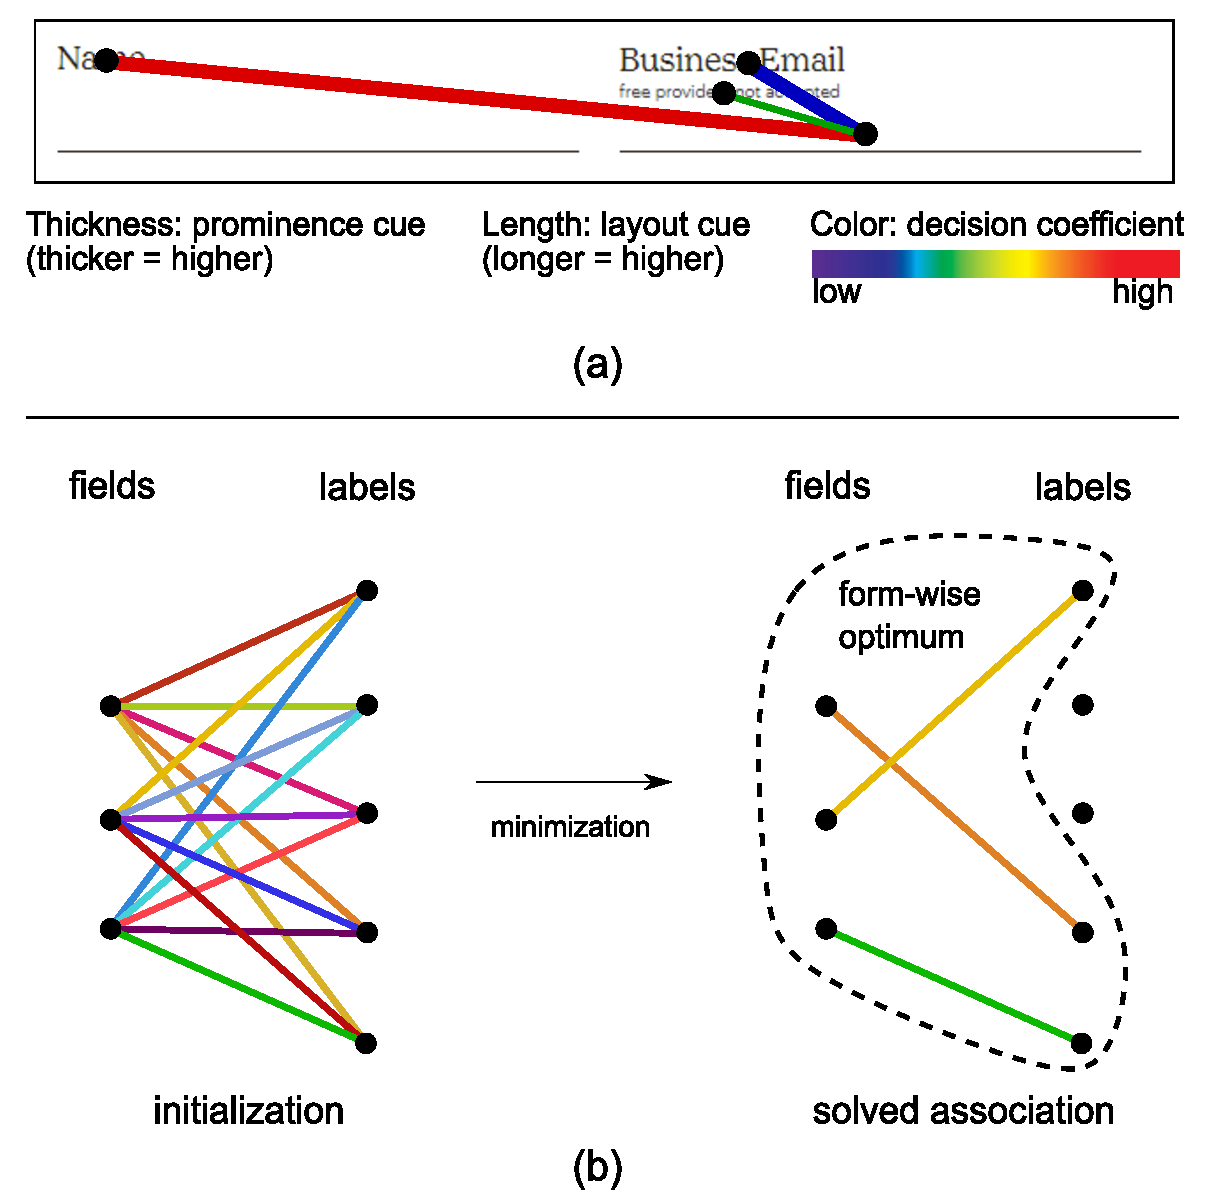
\includegraphics[width=0.86\linewidth]{accessibility_repair/figures/illustration/illustration.pdf}
	\caption{Visualization of (a) the visual cues, and (b) the labeling association. }
	\label{fig:illustration}
\end{figure}

\subsubsection{Decision Variables}
\label{subsec:opt}
Decision variables will be used, in combination with the cues 
gathered from the form, to optimize the assignment of labels. 
The strategy we adopt is to formulate the form labeling analysis 
as a constrained binary program. The rationale for formulating the 
problem in this fashion is as follows. First, the assignment of 
labels must be constrained by other label assignments. That is, 
if a solver has made labeling assignments involving some subset 
of texts, then this should constrain the possible set of texts 
that can be used for remaining labeling assignments for the rest 
of the fields. Furthermore, the labeling assignment can be readily 
expressed as a pair-wise binary function between fields and texts. 
In addition, deciding the form labeling using only individual  
field by field analysis would be a subpar approach. This is because it  
would not consider whether a potential label for a given field might be 
a better match for another field, or whether it was already associated 
with another field. For instance, if field A has equal cue values 
with respect to potential labels X and Y, but field B has optimum 
cue values only with respect to Y, then the optimal decision is to 
assign A to X and B to Y. Having an isolated, field by field analysis 
would not be able to make this decision. In contrast, a global 
combinatorial analysis that takes into account all fields together 
would be a better fit. This is also the reason why the proposed approach 
does not rely on individual cues alone to decide field labeling, but rather 
trades off all cues for all field-label pairs to reach an optimum labeling 
for the form as a whole. For all of the aforementioned aspects, 
a constrained binary program is a potentially suitable approach 
to formulate the labeling problem. 

Accordingly, each decision variable $d_{i,j}$ is a binary value that 
represents the decision of assigning a particular label $t_j$ to a 
particular field $f_i$. \Cref{fig:illustration}(b) illustrates the decision variables. 
On the left hand side of the figure, each line represents one $d_{i,j}$ value. 
Each variable would encode one possibility of labeling. The optimization 
solution, as illustrated on the right hand side of \Cref{fig:illustration}(b), 
represents which decision variables are finally applicable. This is where the 
tradeoff occurs in terms of optimizing various possible combinations of 
visual cues to reach the final labeling. Once all decision 
variables have been determined, the label associated with each field 
is identified. 

\subsubsection{Objective and Constraints}\label{subsec:obj}
In order to create the objective function and constraints, we need to 
consider the kind of labeling markup provided by the ARIA 
standard. This is because the final DOM repair process will include 
generating the necessary markup to convey the inferred labels, and 
this markup has to follow the ARIA standard. The ARIA standard provides 
two types of form labeling: individual and group labels. Individual 
labeling represents the label associated with every single form input 
on its own. For instance, in \Cref{fig:motivating-example}b, individual 
labeling associates the large text area field under 'Message' with the 
label `Message`. For group labeling, consider the two radio option 
fields at the bottom of \Cref{fig:motivating-example}b. The individual 
labels in this case are 'No' and 'Yes', and the group label is `Do 
you have an open ticket`. The strategy we adopt to identify both label 
types is a bottom-up multiple-passes approach. We first infer the 
individual labels, and then use that information to perform another 
pass to identify the group labels. The reason for adopting this 
strategy is that it allows us to optimize the problem for each 
label type separately, and also simplifies group labeling by using 
information from the individual labeling. Therefore, each of these 
label types will have a different objective function and set of constraints. 

Subsequently, each decision coefficient of the optimization is 
calculated as follows: 
\begin{align}
c_{i,j} = \frac{l_{i,j}}{p_i}
\end{align}
where $c_{i,j}$ is the coefficient of the decision variable, $p_i$ is the visual prominence cue, and $l_{i,j}$ is the visual layout cue. The magnitude of each coefficient $c_{i,j}$ describes the 
pair-wise and per-element visual cues. 
The choice of which $i, j$ pairs would constitute a labeling association 
is determined by the objective function and the constraints: 
\begin{equation} \label{eqn:min}
\begin{aligned}
A \; = \; \mathrm{argmin}_{} \; & \sum_{i}\sum_{j} c_{i,j} d_{i,j}   \\
\textrm{s.t.}	\quad & \sum_{j} d_{f_1,j} = 1, \cdots \sum_{j} d_{f_N,j} = 1 \\
							& \sum_{i} d_{i,t_1} \leq 1, \cdots \sum_{i} d_{i,t_M} \leq 1 \\
\end{aligned}
\end{equation}
with $A$ being the labeling associations result. $c$ and $d$ are the coefficients 
and decision variables, respectively, as described in the preceding paragraphs. 
\Cref{fig:illustration}(b) illustrates a number of remarks regarding the above equations. 
First, the color of the lines represent the magnitude of the decision coefficients $c_{i,j}$.  
We can see that the visual cues cover all possible labeling combinations. 
The decision variables then determine which combination of visual cues yields the 
optimal result, as shown on the right hand side of \Cref{fig:illustration}(b). 
We also note that we have two sets of constraints. The first set 
of constraints subjects the optimization to the requirement of finding exactly 
one label. This constraint stems from the ARIA accessibility requirement stating 
that each form field must have a label, and is therefore not assumption or decision 
that we made on our own.  
In \Cref{fig:illustration}(b), only one outgoing line is allowed 
from each field dot. 
Each form field $f$ gets its own constraint equation, containing entries 
for all possible labels. First, this prevents the optimization from yielding the 
trivial solution (i.e., none of the lines in \Cref{fig:illustration}(b) are selected). 
Second, this avoids solutions where only a few fields are 
associated with all labels by virtue of yielding a smaller objective value, 
thereby leaving many other fields without a labeling association. 
For instance, in the solved association in \Cref{fig:illustration}(b) we note that 
the final selection coefficient values are \emph{not} the minimum per each field. That is, 
the final lines on the right hand side are not all blue colored that indicate low coefficient 
values. Rather the final coefficient values are mid-range, illustrating that the 
objective function is seeking the minimum of the whole form, not the individual fields. 
The second set of constraints subjects the optimization to restrictions on the possible 
associations that can be done for text elements. Each text $t$ gets its own 
constraint equation, paired with all possible fields. Paired with the first set 
of constraints, these second constraints enforce a couple of requirements. First, 
that the labeling association for each text entry is optional. That is, it 
encodes the expectation that not every text field present on a form has to be 
a label. We can see this in the solved association in \Cref{fig:illustration}(b) 
where not all the label dots have lines. This is true because forms have many 
texts that are not labels (e.g., descriptions, hints). Furthermore, the constraints 
ensure that each potential label is associated with at most one form field. This enforces the requirement that a solution is not accepted if only a few text elements end up being associated with many fields due to a smaller objective value. 

Once the individual labeling associations are obtained, we proceed to infer the group labeling. First, we discard all texts that have received a labeling association from the individual labeling stage (i.e.,~all $t \in A$). Next, 
our target is to identify groupings of the fields. To achieve this, we take an 
agglomerative clustering approach~\cite{gan_ma_wu_2021}, which is a clustering technique that builds clusters by starting from leaf nodes and than gradually merging groups of nodes. 
The reason for adopting agglomerative clustering is that we use it in a way that enables us to identify groupings without requiring thresholds or parameters. This helps 
in increasing the robustness of analysis, and reduces the often cumbersome manual effort required to tune any parameters. 

We conduct the grouping by first constructing a 
fields distance matrix, whose elements are the visual geometric 
Euclidean distance between each pair of fields. Subsequently, we 
determine the linkage function to be used for the agglomerative 
clustering. This function determines which pair of clusters to 
merge in the next level of agglomeration. For the current task 
of identifying visual groupings, we adopt the single-linkage 
criterion~\cite{gan_ma_wu_2021}. Single-linkage agglomeration 
occurs, in our case, when the minimum visual geometric distance 
between clusters is smallest. 

Accordingly, we run the agglomeration process as per the aforementioned steps. 
We then obtain all heights of the obtained hierarchy of clusters. 
In our case, these heights would signify the progressively increasing visual geometric 
distances between clusters. We then compute the median value of all heights, excluding heights of zero since they don't represent any cluster. This median value is then used as a cutoff to the 
hierarchy of clusters. That is, only clusters whose within-cluster visual geometric distance are below the cutoff are retained. The final result is a set of field groupings.
Once the groupings have been identified, we proceed to infer the labeling associations 
for those groups. We achieve this by performing a second optimization pass and formulate 
the problem as follows:
\begin{equation} \label{eqn:max}
\begin{aligned}
B \; = \; \mathrm{argmax}_{} \; & \sum_{i}\sum_{j} \frac{d_{i,j}}{c_{i,j}}   \\
\textrm{s.t.}	\quad & \sum_{j} d_{f_1,j} \leq 1, \cdots \sum_{j} d_{f_N,j} \leq 1 \\
							& \sum_{i} d_{i,t_1} \leq 1, \cdots \sum_{i} d_{i,t_M} \leq 1 \\
\end{aligned}
\end{equation}
where $B$ is the labeling associations result, 
and $c$ and $d$ are the same variables as those that have 
been used in the first optimization pass, with the exclusion 
of all individual labeling associations that have been obtained 
from that first pass. We make a number of remarks regarding the 
above equations. First, we note that the structure of the 
problem is different from that in the first optimization pass. 
We now have a maximization problem instead of a minimization. 
The rationale for this is as follows. 
First, we note that individual labels are always present while 
group labels may or may not be present~\cite{ARIA}. 
The problem formulation therefore needs to take this into account. 
This brings us to the second observation, which is regarding the 
constraints. In the previous pass, we had constraints to have 
the decision variables finding exactly one label (i.e. the 
equality constraints). In this pass, however, no such requirement 
is made. Instead, we have an upper bound inequality constraint 
on the decision variables pertaining to all form fields (the 
first set of constraints in \Cref{eqn:max}). This encodes the 
fact that group labeling associations may or may not be present 
on a given form, and if it does have one, that its doesn't result 
in a degenerate case where many texts are associated with a given 
field. However, since we now have an upper bound inequality 
instead of an equality constraint, the problem can no longer 
remain a minimization. This is required in order to avoid trivial 
solutions (i.e. zero decision variable selections). Accordingly, 
the problem is formulated as a maximization. The placement of 
the coefficients of decision variables have been adjusted accordingly 
to reflect the change in the objective. However, their computation 
remains the same as before, using the same visual cues we previously 
described. We also note that the second set of constraints 
(pertaining to the text elements) have remained the same as before, 
since we still have the same expectation as the first case that 
not all texts need to partake in a labeling association. 

\subsection{DOM Augmentation Markup}
So far, the form has been abstracted, visual cues generated, and 
the optimizations yielding the labeling associations have been 
solved. At this stage, we perform the final step needed to ensure 
form labeling accessibility, which is repairing the DOM. 
This stage involves transforming the labeling associations into 
ARIA accessibility markups. These markups are finally added to 
the DOM of the page in order to explicitly encode all labels.  

The ARIA standard provides markup for both individual and group 
labels. We will start by describing the encoding for individual 
labels, and then proceed to describe to the case of groups. 
First, we take all the individual labeling associations obtained in 
$A$ (\Cref{eqn:min}).  This provides a mapping of $f_i$ to $t_i$, 
representing pairs of fields and labels, respectively. Next, we 
iterate over each field $f_i$, and examine the associated label 
$t_i$. If the $t_i$ element in the page has an id (i.e. a non-zero 
\code{id} attribute), then we obtain that id. Otherwise, a unique 
random id is generated for that element and added as an \code{id} 
attribute for that element in the DOM. Subsequently, for each field 
$f_i$, we add the \code{aria-labelledby} standard ARIA attribute. 
The value of this attribute is then set to the value of the \code{id} 
attribute of the associated $t_i$, whether that id already exists 
or was generated. If the associated $t_i$ is not an explicit element 
(e.g., the text is contained in an attribute), then we add an 
\code{aria-label} instead of \code{aria-labelledby}, and we set its 
value to be the content of the text, since assigning an id in this 
case is not possible. The ARIA standard allows labeling elements 
using both ids and the actual textual value of the label. 

We then move on to process the group labeling associations 
obtained from $B$ (\Cref{eqn:max}). In this case, the mapping 
result is different from the case of individual labeling 
associations. Here the mapping is from a set of fields 
$\{f_1, \ldots, f_n\}$ to the associated inferred label 
$t_i$. We begin by iterating over each set of fields, and 
examine the associated label. We obtain the id of the associated label, 
or generate a unique one if it does not exist, in the same 
fashion as done in the previous case for individual labels. 
Next, we find the \emph{nearest common ancestor} in the DOM 
for the $\{f_1, \ldots, f_n\}$ set. The reason for doing this 
is the nature of the standard ARIA attribute used to group 
related elements, which is \code{role="group"}. It should 
contain as descendants the group of elements its representing~\cite{aria-group-markup}. 
Accordingly, for the nearest common ancestor node of a set $\{f_1, \ldots, f_n\}$, 
we add the attribute \code{role="group"} to that node to 
communicate the presence of a labeling group. Next, we add 
the \code{aria-labelledby} attribute to the same nearest common 
ancestor node, and set the value of the attribute to the id 
attribute (whether existing or generated) of the mapped label $t_i$ 
associated with the set $\{f_1, \ldots, f_n\}$. Finally, we note 
that the markup repair process can be executed at any time, 
whether on page load, or whenever the DOM of the form is updated 
in dynamic pages. 


\header{Implementation}
We implemented the proposed approach using server-side JavaScript 
(Node). We used the Selenium WebDriver to instrument browsers and 
extract DOM information and computed attributes. To make the study 
replicable, we made available online a link to our data and 
tool~\cite{tool-and-data}, which we called~\toolname (short for 
accessible forms). We used OpenCV~\cite{opencv} for image operations 
and Lpsolve~\cite{lpsolve} to formulate and solve the optimizations. 


\section{Evaluation}

\label{sec:evaluation}
We conducted qualitative and quantitative studies  
to answer the following research questions:

\begin{enumerate}[label=\textbf{RQ\arabic*},leftmargin=*]
	\item How accurate is the labeling associations inference? 

	\item How safe is the labeling markup repair process?
	
	\item How scalable is the performance with the size of 
	real-world web forms? Is it suitable for real-time usage?
\end{enumerate}

In the following subsections, we discuss the details of the experiments that 
we designed to answer each research question, together with the results and discussions.

\subsection{RQ1: Inference Accuracy}\label{subsec:rq1}
In this question, the objective is to assess how accurate 
is the inference of the labeling associations in a given web form. 
We recall that, as per the ARIA standard, a web form is accessible 
if it has markup that correctly captures the labels on the form. 
Accordingly, the most important evaluation question is to 
assess how accurate are the inferred form labels. 

We evaluated this research question as follows. 
First, we collected 30 random subjects that were sourced 
from the Alexa top websites list~\cite{alexatop}. 
The way we selected the evaluation subjects are as follows. 
To start, we get a random subject url from the pool. 
We then load that url in a browser in order to inspect the website. 
This inspection process is conducted manually, and its goal is to 
find a page on the website that contains a web form. 
For each website, we manually inspect its various sections and pages 
until a web form is found. If no web forms are found within five minutes 
of manual examination, the subject is skipped and a new random url 
is obtained from the pool. The only additional criterion we have on web forms 
is that they are reachable without requiring registration or payment. 
This criterion was made in order to simplify the process of collecting 
subjects. The final list of subjects is shown in \Cref{table:subjects}, 
and the full urls are available online~\cite{tool-and-data}. 
The final list of subjects covers a variety of tasks from 
many categories of websites (e.g. news, education, commerce), 
with a varying number of elements in forms, ranging from 17 up to 1552, 
which covers around two orders of magnitude of form sizes. This 
variety of topics and size ranges helps in having a more 
representative and generalizable evaluation. 
Subsequently, we feed the web form to our approach and obtain 
the output labeling associations. We then examine each generated 
association and classify the results into true positives, 
false positives, and false negatives. 
In false positives, the inferred labeling association for 
a given field does not match the visually perceived labeling. 
For instance, in \Cref{fig:motivating-example}b, if the 
inferred labeling associates the selected radio button to 
the label `Yes`, then this is a false positive labeling, 
because it does not match the correct visually perceived 
labeling, which is the `No` option. 
Next, in true positives, the inferred labeling association 
for a given field correctly matches the visually perceived 
labeling. For instance, in \Cref{fig:motivating-example}b, 
if the inferred labeling associates the large text area 
input to the label `Message`, then this is a true positive labeling. 
Finally, false negatives are cases in which no labeling 
associations were inferred for a field that should have 
been associated with a label. For instance, in \Cref{fig:motivating-example}b,
if no labels were associated to the first text field input, 
then this is a false negative, because there should 
have been a label (i.e., `Name`). 

Finally, in order to have a more thorough and informative evaluation, we include a baseline in our experiments. 
While we could simply present the evaluation from just the approach 
itself, this would not provide context as to how it would 
perform compared to other potential solutions, and therefore 
adding a baseline helps in making the evaluation more meaningful. 
However, as discussed in the introduction, 
existing works only test the accessibility of markups, but do not 
conduct any inferences or repairs of form labeling~\cite{yesilada2019web, ukgov:audit:2018}. 
They assert that accessibility attributes are not empty, 
while the proposed analysis in this chapter infers what \emph{values}  
should be assigned to the form labeling attributes. 
Accordingly, no comparable tool exists that can be included in the evaluation, and 
therefore the next best option is to have a random selection process as the baseline. 
In this process, random elements from a given web form are selected. 
Next, a labeling association is generated to another randomly selected form element. 
This set of randomly selected elements and their associations 
is then taken to be the baseline.

%\noindent\begin{minipage}[t]{\linewidth}
\renewcommand{\arraystretch}{0.7}
\begin{table}
\caption{List of the 30 subjects used for evaluation.}
\label{table:subjects}
\centering
\begin{tabularx}{0.85\columnwidth}{llrr}
\hline
\small \textbf{Subject}  &  \small \textbf{Form} 						& \small \textbf{\# elements}  & \small \textbf{total \#} 		\\ %	& \textbf{total} \\ 
\small \textbf{}  &  \small \textbf{description} 			& \small \textbf{in form}  		& \small \textbf{elements} 			\\ %	& \textbf{size, KB} \\ 
\hline
\footnotesize wikipedia.org     & \footnotesize Page links search   					&	\footnotesize	45     						  &	\footnotesize 518				\\ %				&	227.1				      \\
\footnotesize opinionlab.com    & \footnotesize Experience feedback      &		\footnotesize 116     						  &	\footnotesize 136							\\ %	&	15.6				      \\     	   
\footnotesize zoom.us           & \footnotesize Live demo request      				&		\footnotesize 437     						  &	\footnotesize 924				\\ %				&	200.0		    \\           
\footnotesize netflix.com       & \footnotesize New titles suggestion      			&	   \footnotesize 17     						  &	\footnotesize 432			\\ %			&	148.6			 \\            
\footnotesize microsoft.com     & \footnotesize Careers support ticket      		&		\footnotesize 86     						  &	\footnotesize 444				\\ %		&	140.6			      \\           
\footnotesize dropbox.com       & \footnotesize Business account inquiry      		&		\footnotesize 398     						  &	\footnotesize 721			\\ %			&	130.2		      \\           
\footnotesize stackoverflow.com & \footnotesize Help center      						&     \footnotesize 106     						  &	\footnotesize 743				\\ %			&	106.7		      \\            
\footnotesize etsy.com          & \footnotesize Product design careers      		&		\footnotesize 68     						  &	\footnotesize 340				\\ %			&	347.9		      \\            
\footnotesize zendesk.com       & \footnotesize Customer service inquiry      		&	   \footnotesize 428     						  &	\footnotesize 1323			\\ %			&	209.6		      \\            
\footnotesize bing.com          & \footnotesize  Search customization     &	   \footnotesize 1552     					  &	\footnotesize 1642						\\ %		&	289.0		      \\          
\footnotesize github.com        & \footnotesize Account support request     		&	   \footnotesize 229     						  &	\footnotesize 283				\\ %			&	42.8	      \\           
\footnotesize intuit.com        & \footnotesize Career events sign-up      			&	   \footnotesize 326     						  &	\footnotesize 1293			\\ %		&	201.5		      \\           
\footnotesize salesforce.com    & \footnotesize Website quality feedback      		&	   \footnotesize 102     						  &	\footnotesize 764			\\ %		&	279.9				      \\            
\footnotesize indeed.com        & \footnotesize Account registration      			&	   \footnotesize 54     						  &	\footnotesize 222				\\ %		&	47.0				      \\            
\footnotesize paypal.com        & \footnotesize Search for jobs      					&		\footnotesize 144     						  &	\footnotesize 410			\\ %		&	48.55				      \\            

\footnotesize coursera.org		& \footnotesize Services inquiry	&  \footnotesize 569  & \footnotesize 1210 \\
\footnotesize glassdoor.com		& \footnotesize Sales specialist contact	& \footnotesize 1536	& \footnotesize 1864	\\
\footnotesize insiderintelligence.com	& \footnotesize Subscription request &	\footnotesize 391	& \footnotesize 1019	\\
\footnotesize formstack.com		& \footnotesize Violations reporting	& \footnotesize 126	& \footnotesize 182	\\
\footnotesize dailymail.co.uk	& \footnotesize Message board help	& \footnotesize 45	& \footnotesize 986	\\

\footnotesize squarespace.com	& \footnotesize Press contact	& \footnotesize 33	& \footnotesize 725	\\
\footnotesize elsevier.com		& \footnotesize Advertising request	& \footnotesize 437	& \footnotesize 940	\\
\footnotesize hootsuite.com		& \footnotesize Community enrolment	& \footnotesize 61	& \footnotesize 560	\\
\footnotesize flickr.com		& \footnotesize Support ticket request	& \footnotesize 243	& \footnotesize 348	\\
\footnotesize goodreads.com		& \footnotesize Advertising inquiry	& \footnotesize 75	& \footnotesize 551	\\

\footnotesize slack.com			& \footnotesize Sales contact	& \footnotesize 461	& \footnotesize 1087	\\
\footnotesize evernote.com		& \footnotesize Teams products inquiry	& \footnotesize 298	& \footnotesize 730	\\
\footnotesize udemy.com			& \footnotesize Demo request	& \footnotesize 50	& \footnotesize 241	\\
\footnotesize blackboard.com	& \footnotesize Personalized experience	& \footnotesize 641	& \footnotesize 838	\\
\footnotesize mailchimp.com		& \footnotesize Report compliance issues	& \footnotesize 58	& \footnotesize 1209	\\  

\end{tabularx}
\end{table}
%\end{minipage}

\subsubsection{Results and Discussion}
\Cref{table:rq1} shows the results of evaluating the accuracy 
of inferring web form labeling. 
The table has two groups of columns, ``Proposed approach'' 
and ``Baseline'', 
showing the accuracy of inference for both methods, respectively. 
The key outcome of this table is the F-1 measure, 
which is at 89\% for the proposed approach. 
This indicates a rather effective inference process. 
Precision and recall were comparable, at 88\% and 89\%, 
respectively. 
\Cref{fig:label-pairs} shows a sample of the inferred labeling 
associations corresponding to the motivating example. Each 
entry represents a mapping from a particular field to a particular label.

%\noindent\begin{minipage}[t]{\linewidth}
\renewcommand{\arraystretch}{0.7}
\begin{table}[t]
\caption{Evaluation of the inference accuracy of labeling associations.}
\label{table:rq1}
\centering
\begin{tabularx}{0.85\columnwidth}{p{0.2\textwidth}rrr|rrr}
\hline
                  & \multicolumn{3}{c|}{\textbf{\small Proposed}}                                      & \multicolumn{3}{c}{\textbf{\small Baseline}}                                          \\
                  & \multicolumn{3}{c|}{\textbf{\small approach}}                                      & \multicolumn{3}{c}{}                                                \\
\hline
\textbf{\small Subject}           & \multicolumn{1}{c}{\textbf{\small TP}} & \multicolumn{1}{c}{\textbf{\small FP}} & \multicolumn{1}{c|}{\textbf{\small FN}} & \multicolumn{1}{c}{\textbf{\small TP}} & \multicolumn{1}{c}{\textbf{\small FP}} & \multicolumn{1}{c}{\textbf{\small FN}}  \\ 
\hline
\small wikipedia.org     & 3                       & 0                       & 0                       & 0                       & 5                       & 1                        \\
\small opinionlab.com    & 6                       & 2                       & 0                       & 0                       & 11                      & 1                        \\
\small zoom.us           & 12                      & 0                       & 2                       & 0                       & 13                      & 4                        \\
\small netflix.com       & 3                       & 0                       & 2                       & 1                       & 4                       & 3                        \\
\small microsoft.com     & 5                       & 0                       & 0                       & 0                       & 15                      & 0                        \\
\small dropbox.com       & 9                       & 0                       & 1                       & 0                       & 7                       & 4                        \\
\small stackoverflow.com & 4                       & 1                       & 0                       & 0                       & 6                       & 1                        \\
\small etsy.com          & 3                       & 0                       & 2                       & 0                       & 2                       & 3                        \\
\small zendesk.com       & 6                       & 0                       & 0                       & 0                       & 9                       & 1                        \\
\small bing.com          & 11                      & 7                       & 1                       & 0                       & 5                       & 4                        \\
\small github.com        & 5                       & 0                       & 0                       & 0                       & 9                       & 2                        \\
\small intuit.com        & 6                       & 0                       & 0                       & 1                       & 7                       & 2                        \\
\small salesforce.com    & 3                       & 1                       & 1                       & 0                       & 8                       & 1                        \\
\small indeed.com        & 5                       & 2                       & 1                       & 0                       & 6                       & 2                        \\
\small paypal.com        & 4                       & 0                       & 0                       & 1                       & 3                       & 1                        \\
\small coursera.org			& 12	& 0		& 1		& 0		& 6		& 5 \\
\small glassdoor.com			& 7		& 0		& 3		& 0		& 5		& 3 \\
\small insiderintelligence.com	& 7		& 3		& 0		& 0		& 4		& 6 \\
\small formstack.com			& 6		& 1		& 0		& 0		& 3		& 5 \\
\small dailymail.co.uk			& 8		& 0		& 1		& 1		& 4		& 3 \\
\small squarespace.com			& 5		& 1		& 0		& 1		& 5		& 1 \\
\small elsevier.com			& 15	& 1		& 2		& 0		& 6		& 10 \\
\small hootsuite.com			& 5		& 0		& 0		& 0		& 4		& 1 \\
\small flickr.com				& 6		& 1		& 2		& 0		& 3		& 6 \\
\small goodreads.com			& 7		& 0		& 1		& 0		& 2		& 5 \\
\small slack.com				& 10	& 2		& 2		& 0		& 8		& 4 \\
\small evernote.com			& 6		& 1		& 0		& 0		& 4		& 3 \\
\small udemy.com				& 7		& 0		& 0		& 1		& 3		& 3 \\
\small blackboard.com			& 13	& 3		& 1		& 0		& 5		& 11 \\
\small mailchimp.com			& 8		& 1		& 1		& 0		& 6		& 4 \\
\hline
						& Prec.						  & Rec.							 & F1							   & Prec.						  & Rec.							 & F1				 \\
						& 88.4\%						  & 89.6\%						 & 89.0\%						& 3.3\%					 	  & 5.7\%						 & 4.1\%			 \\

\end{tabularx}
\end{table}
%\end{minipage}
























In order to further understand the limitations of the approach, 
we investigated the false positive and false negative cases. 
We identified a few trends. First, false positives occurred in 
forms that had visual prominence cues that did not follow the 
proposed optimization model (\Cref{{subsec:obj}}). In these 
cases, the forms had a high ratio of texts relative to fields 
and all the texts had similar visual prominence cues. This 
resulted in the optimization process yielding suboptimal 
labeling associations. False positives also occurred in cases 
where, in addition to the aforementioned similarity in visual 
prominence, the visual layout was dense, which made it difficult 
to compensate for the layout density using visual prominence information. 

As for the false negatives, the most predominant case was due to 
non-standard form elements. That is, these cases did not follow 
the normal practice of using input tags to indicate form fields. 
The most common example of this case is Captcha elements 
(e.g.,~``I'm a human" checkboxes), which are designed on purpose to avoid 
being detected by automated tools as form fields.  
Such elements are only styled to appear, for instance, as a 
checkbox when observed by sighted users. For these reasons, 
existing studies~\cite{moreno2014captcha,noorjahan2019bio} have 
also confirmed these hindrances of accessibility due to Captcha elements. 
The proposed approach is incapable of handling these cases. 
For future work, a potential solution to this problem might include 
formulating another set of visual cues to detect the missed cases, 
or exploring the use of a deep learning detector.   

We also examined the effect of form size on the inference accuracy, 
as shown in \Cref{fig:stratified}. The figure shows the average F1 
score of inference for three different groups of form sizes, which 
are the 0 to 33, 33 to 66, and 66 to 100 percentile of form sizes as 
measured by the number of DOM elements in the form. First, we note 
that the first group had slightly lower inference accuracy compared 
to the second group. But we do know that the number of false positives have stayed the same, and therefore the lower accuracy can be attributed to the arithmetic of computing accuracy, where a single inference error in a form with a small number of elements would impact the accuracy more so than a single inference error among a large number of form elements. Second, we note that the lowest accuracy was for the last group (i.e., largest forms). This is due 
to the observation mentioned in the preceding paragraphs, where the 
larger forms tend to have a more dense visual layout, which reduced the 
quality of the optimization decisions as the cues became less 
discriminating due to the higher layout density. However, 
the observed reduction in accuracy is not that significant, and we 
emphasize that all the aforementioned observations are relative in 
nature with respect to the other size groups. Accordingly, the key 
observation of this evaluation is that the inference accuracy remains 
relatively stable across size ranges in \Cref{fig:stratified}.

\begin{figure}
    \noindent
	\begin{minipage}[c]{.97\columnwidth}
        \centering
        \begin{lstlisting}[language={JavaScript},frame=ltbr,aboveskip=1.1em,basicstyle={\linespread{0.8}\footnotesize\ttfamily},]		
{	// associations.json
	// each entry is xpaths of field -> label 

	".../form/textarea[@id='bx_3978']": 
			".../form/div[1]/p", // <p>Message</p>
	
	".../form/input[@id='vr_9481']": 
			".../form/section[1]/div[1]/p", // <p>Name</p>
	
	".../form/select[@id='frq']": 
			".../form/section[2]/div[2]/p", // <p>How often ...</p>
	
	// remaining elements ...
}\end{lstlisting}
    \end{minipage} \hfill
\caption{Sample of the generated association decisions output (corresponds to \Cref{fig:motivating-example}).}
    \label{fig:label-pairs}
\end{figure}

\subsection{RQ2: Markup Safety}\label{subsec:rq2}
In the previous research question, we examined how accurate the labeling 
association inference is. 
Once that aspect has been evaluated, we need to examine whether 
the insertion or augmentation of the inferred associations into the 
DOM is safe. 
The rationale for evaluating this aspect is that we want to make 
sure that any markup repairs applied to a page does not 
cause any unintended or unaccounted for breakages or failures to the page. 

We evaluated this research question as follows. 
First, we continued using the same test subjects used in the first 
research question. Each subject is then loaded in a browser 
and had their labeling associations inferred and the DOM repaired. 
To assess the safety, we check two different aspects. First, 
a visual check is made comparing images of the page before and 
after the repair. The rationale is to assess whether the generated 
markup would cause unintended breakage to the rendering of the page. 
Second, a functionality check is made. Here, we randomly manipulate 
the form (e.g., we select various radio options, expand different drop down menus) to assess whether the generated markup caused  unintended breakage to the form. Breakages might occur, for instance, if the generated markups are incorrect, or break some element or attribute dependencies in the script of the page. Finally, we note down the outcome (i.e., pass or fail), and note down the number of failures. 


\subsubsection{Results and Discussion}
\Cref{table:rq2} shows the results of evaluating the safety of 
the markup repair. For each subject, the columns show the 
outcome of the safety check and the number of failures. Subjects 
for which no failures were observed have `-' under the number of 
failures column. For most subjects, we did not observe any failures. 
For two of the subjects, as shown in \Cref{table:rq2}, we did 
observe failures. In both these cases, the DOM repair process  failed. The reason for these failures is locator breakages. This occurs 
because after the labeling association for a field is determined, 
locators are used locate the field in the DOM, then insert the markup 
repairs at that location. But in the case of the observed failures, 
the locators became stale, where locators that were 
previously valid become unusable. This occurred because the subject's 
DOM was highly dynamic and therefore the DOM has changed 
since the time the locator was acquired. In this work we used DOM 
locators in the form xpath strings. The issue of stale locators 
and possible approaches to address them have been also reported in 
other web testing and analysis works~\cite{leotta2016robula, kirinuki2019color} 
and is still an open research problem. 
For future work, we plan to explore different possibilities to capture 
the locators and address these issues. One option would be devising a 
more robust timing strategy at which to capture the locators in order to 
minimize the probability of going stale. Another option would be using 
visual locators instead of DOM locators. 
 
%\noindent\begin{minipage}[t]{\linewidth}
\begin{table}[t]
\caption{Evaluation of accessibility markup augmentation safety.}
\label{table:rq2}
\centering
\begin{tabular}{llr}
\hline
\textbf{Subject}    & \textbf{Outcome} 		&\textbf{\# failures} \\ 
\hline
paypal.com        	& fail      			&		3             \\
intuit.com        	& fail      			&		2             \\
remaining subjects	& pass	  				& 		- 			  \\
\hline
\end{tabular}
\end{table}
%\end{minipage}    

\subsection{RQ3: Runtime Scalability}\label{subsec:rq3}
After evaluating the accuracy and safety aspects in the previous 
research question, this question examines the runtime performance (i.e., 
total time of execution). 
The rationale for evaluating this question is as follows. 
First, since a couple of aspects in the optimization formulation 
are combinatorial in nature, we wanted to assess whether or not this 
is going to cause any performance penalty, and more importantly how does 
the performance scale with the size of forms. 
Second, since the goal of this work is to make web forms accessible, 
it would be useful to know if the runtime performance is good enough 
if this approach were to be used for real-time repair by end users 
during their browsing activities. 

We evaluated this research question as follows. 
For each subject, we record the number of DOM elements in the forms 
as a measure of form size. We are measuring the elements in the form 
since our approach only focuses on form regions within the page, 
and is therefore not impacted by the rest of the page.
This will be used to measure how does the runtime scale with form size. 
Then, the total runtime is measured from the moment the subject is loaded 
until the final DOM markup is augmented. 

\subsubsection{Results and Discussion}
\Cref{fig:rq3} shows the results of the runtime performance evaluation. 
The x-axis is semi-log and shows the number of DOM elements within 
the form. The y-axis is linear and shows the runtime in milliseconds. 

The average runtime is $1667 \pm 532$ milliseconds. Minimum and 
maximum runtimes are 1044 and 2733 milliseconds, respectively. 
The data range of DOM elements covers around two orders of magnitude 
of form sizes, making it suitable for assessing scalability.
The runtime scales roughly linearly with the size of the DOM, 
indicating good scalability with respect to form complexity.  
We recall that we are implementing the optimization in the Lpsolve~\cite{lpsolve} 
solver. While the solver is a good fit for the type of optimization 
we are conducting, it is known to be lacking in terms of runtime 
performance~\cite{luppold2018evaluating}. Accordingly, while the 
observed average performance of around 1.6 seconds is arguably 
suitable for run-time repair, the performance will likely improve 
further when more capable solvers are used, and therefore the 
current evaluation is a conservative estimate. The key outcome, 
however, remains the same, which is that the proposed web form 
analysis scales linearly with respect to form complexity. This 
provides some indication that the formulated optimization problem 
and constraints do not practically result in a combinatorial 
explosion that would cause computationally prohibitive analysis.   

\begin{figure}
	\centering
	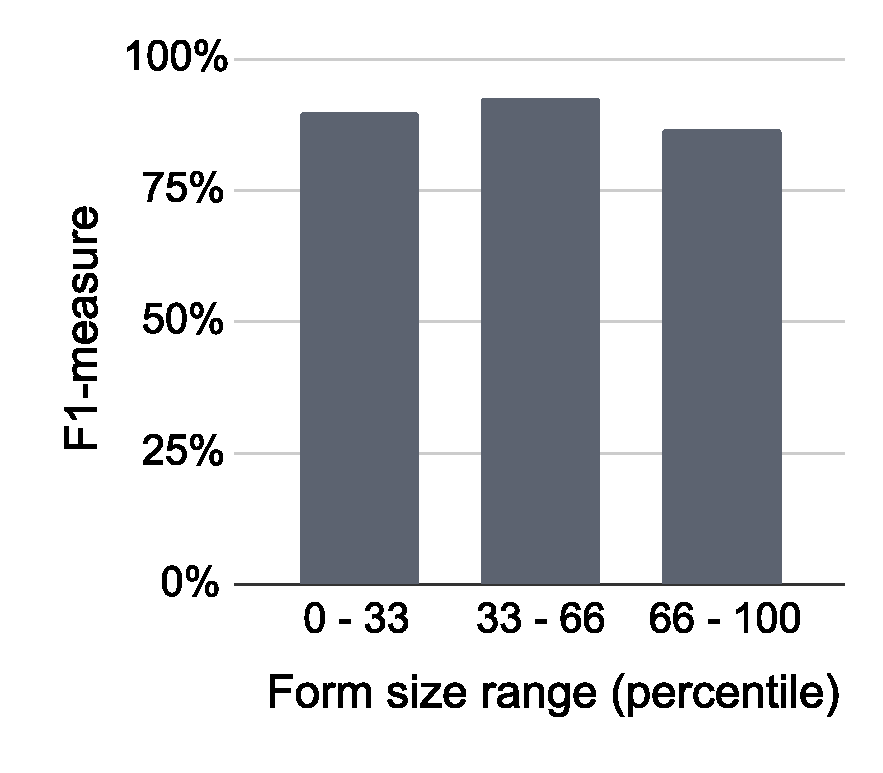
\includegraphics[width=0.45\linewidth,trim=11mm 9mm 7mm 7mm,clip]{accessibility_repair/figures/stratified.pdf}
	\caption{Comparison of labeling inference F1-measure for different form size ranges.}
	\label{fig:stratified}
\end{figure}

\subsubsection{Threats to validity}
In order to avoid any selection bias, 
we chose test subjects (i.e., web sites) 
randomly with the mentioned 
criteria in \Cref{subsec:rq1}. 
The subjects cover diverse categories 
(e.g. news, education, commerce), 
with around two orders of magnitude of 
form sizes, ranging from 17 up to 1552 elements.
This diversity of topics and sizes helps in 
ensuring subjects are representative 
of real-world scenarios, thereby mitigating the 
external validity of the study by making the 
results generalizable.
To make the study replicable and mitigate researcher bias, 
we made available online a link to our tool 
implementation and evaluation data~\cite{tool-and-data}.




\begin{figure}
	\centering
	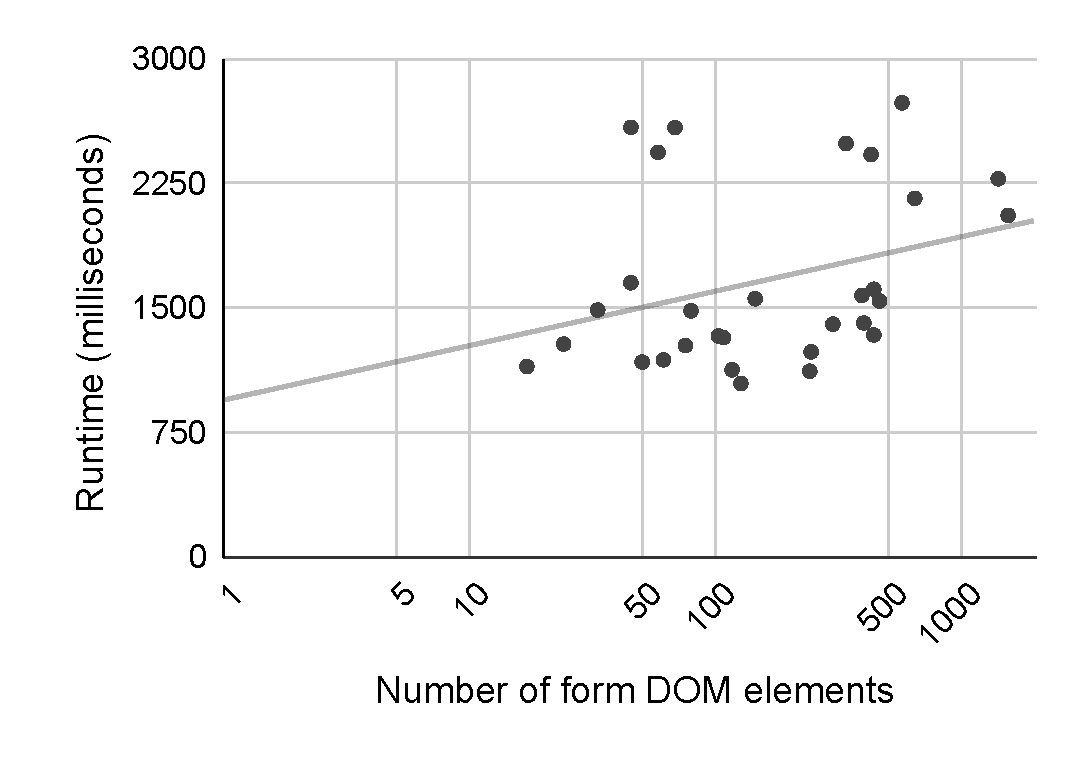
\includegraphics[width=0.7\linewidth,trim={8mm 12mm 8mm 8mm},clip]{accessibility_repair/figures/rq3chart.pdf}
	\caption{Evaluation of the runtime performance scalability for various sizes 
		of input web forms. (Runtime in milliseconds. Form size in number of DOM elements in a form.)}
	\label{fig:rq3}
\end{figure}

\section{Related Work}
A number of tools exist for repairing or improving a few accessibility 
issues~\cite{yesilada2019web, asakawa2019transcoding}. 
One common accessibility improvement approach is already 
in use in modern web browsers, 
such as allowing users with low-vision (e.g., mild vision problems, 
color blindness) to override the default CSS stylesheet into more 
contrasting colors in order to improve their visual perception of 
the page, or to zoom in to the page in order to be able to better 
see its content. Another line of work aims at suggesting alternative 
texts for images to make them accessible~\cite{mack2021designing, 
wu2017automatic, bigham2006webinsight}, building on the abundant 
and extensive deep learning research on the task of image 
captioning~\cite{hossain2019comprehensive}. Accessibility improvements 
have also been proposed based on restructuring of web page regions with 
the goal of prioritizing key sections so that they become more prominent 
and easier to access~\cite{akpinar2015old}.

However, there is little to no work in the literature in terms of a 
software analysis approach that infers and repairs missing web form 
DOM labeling markup, which is one of the most common web accessibility 
errors~\cite{webaim:1mil}. This is the research problem that the presented approach addresses. 

Another line of work focuses on accessibility testing~\cite{abascal2019tools, 
ukgov:audit:2018}, which is generally based on performing syntactic checks 
that consist of basic rules, such as:  any \code{ul} list element must contain 
non-empty \code{li} child elements, or no \code{input} elements must not be 
descendent of \code{a} elements. The goal of such checks is to provide quick 
and simple assertions that are easily automatable.
Patil et al.~\cite{patil2016enhanced} and Eler et al.~\cite{eler2018automated} 
check for absence of predefined attributes in mobile applications, 
such as the absence of required alternative text for all user interface images. 
These are then flagged and reported to developers, allowing them to identify 
and fix these potential issues. Other tools~\cite{aslint_tool,goog_scanner} 
perform similar syntax checks, differing mainly in what attributes are being checked. 
None of these works, however, perform repairs. 

The majority of existing software accessibility related research  
come from a human factors research perspective, rather than from a 
software engineering or tooling perspective.
For instance, one line of work~\cite{snider2020accessibility, alshayban2020accessibility, 
yan2019current, bhagat2019evaluation,ross2018examining,agrawal2019evaluating,dominguez2018website} 
is based on analyzing existing websites (or categories of websites, 
such as educational or banking) by manually 
observing how non-sighted users would interact with them. 
The goal is to discover any issues that might surface during usage, 
and then come up with improved accessibility guidelines. 
The hope is that these guidelines will be later kept in mind while 
developing software. 
A related area of research aims to discover how the software development 
practices themselves can be improved such that it is more likely that 
the end product software is more accessible. 
Krainz et al.~\cite{krainz2018can} explores how model-based development 
contributes to accessibility compliance. 
Sanchez et al.~\cite{sanchez2017method} and Bai et al.~\cite{bai2018categorization, 
bai2019methods} focus on agile software engineering practices and how do they 
impact the accessibility of the product.  

Another line of research is concerned with generating inputs for 
testing purposes~\cite{adamo2018combinatorial,su2017guided}. 
These works have proposed techniques geared towards improving 
the generation, utility, or robustness of test inputs. 
One goal of this vast area of research is to create better 
sequences of test operations or test data with the goal of 
achieving a certain testing objective (e.g., increased coverage). 
\cite{song2017ehb, sadeghi2017pat} adopt a strategy 
of randomly generating the inputs. 
In these cases, the focus is not mainly on the generated input 
data itself but on other aspects of testing, such as improving 
how the event space is traversed or how to better generate 
assertions, with the raw input data being randomly generated, 
or predefined by the user. Another line of work~\cite{arnatovich2018mobolic, 
dhok2016type} gives more attention to the raw input data. 
In these cases, specific types or formats of input values 
are used instead of randomly generated inputs. 
The intuition is that properly formatted and typed inputs 
allow better exploration and testing. 
The aforementioned works, however, are not related to accessibility 
testing or repair, nor aim at generating the required labeling 
associations to be able to perform accessibility repair.  

Finally, a few existing works have explored the use of some visual analysis 
aspects for testing or analyzing web applications. 
Burg et al.~\cite{burg2015explaining} propose a program understanding tool 
that is geared towards front-end development projects and understanding how 
the user interface changes during interactions with the application. It allows 
a developer to select a certain element that 
they are interested in, and the tool tracks how the UI is changing with respect to 
that element, and tracks the corresponding code changes. 
Bajammal et al.~\cite{bajammal2018generating} analyzes the UI of a web page in 
order to generate reusable components, based on patterns in design mockups or templates.  
Choudhary et al.~\cite{choudhary2012crosscheck} focuses on cross-browser 
compatibility, and proposes a technique that checks for difference between 
how a given web page is rendered across browsers. A given web app is loaded in two 
different browsers, and an image diff is performed to locate the areas where 
the two browsers differ, therefore helping the developer to identify issues 
that may not otherwise be easy to identify. 


\section{Conclusion}

Filling web forms is a key activity when browsing the web. 
While this task is routine for sighted users, 
it presents a significant hurdle for non-sighted users if the form does not 
contain the required DOM accessibility labeling markup. This 
issue of missing labeling markup is one of the most common accessibility 
errors. However, 
when a non-sighted user is faced with missing form labeling, 
there are currently little to no options available to access 
that form. To this end, this chapter proposed a software analysis approach 
that automatically analyzes web forms and infers their labels to make them accessible. 
The approach first abstracts a given web form, then generates 
visual cues from the form. These cues are then used in an optimization 
model to solve for the form labeling associations. These are 
finally translated into standard ARIA accessibility markups and augmented into 
the DOM to repair the form and make it accessible. 
We evaluated our approach on 30 real-world subjects 
and assessed the accuracy of labeling inference, the safety of 
the DOM augmentation repairs, as well as the labeling performance. 
The results show an average F1-measure of 88.4\% for label 
inference, and an average run-time of around 1.6 seconds.


%\bibliography{IEEEabrv,bibliography}
\chapter{Generating web UI components}
\label{chp:maintainability}

%% !TEX root =  paper.tex

\section{Introduction}
\label{section:introduction}

The development of user interfaces (UIs) for web apps is often a manual and time 
consuming task.In a survey of more than 5,700 developers, 51\% reported working 
on app UI design tasks on a daily basis~\cite{IDC:survey},
more so than other development tasks, which they tended to perform every few days. 
Another study also showed that an average of 48\% of the code size of software is 
related to the user interface~\cite{myers:ui:survey}.

A common workflow for creating web user interfaces 
is \textit{mockup based design}~\cite{Newman:2000:SitemapsStoryboardsSpecifications, Ozenc:2010:SupportDesigners}.
In this approach, a graphic designer creates a rough illustration of the anticipated UI design, called the \textit{mockup} or \textit{wireframe},
usually through a graphic design software or a WYSIWYG editor. 
This mockup is then exported to \html to be rendered in a browser.
A web developer then examines the mockup and begins constructing web components for the app, which are nowadays implemented in one of the popular front-end frameworks such as \angular~\cite{Angular} or \react~\cite{React}.

\renewcommand{\toolname}{\textsc{VizMod}\xspace}
The main building block of UI design, and a cornerstone of these front-end frameworks, is the concept of  
\textit{reusable components}~\cite{React-components, Angular-components},
which are a set of APIs and coding practices allowing reuse and encapsulation of repeated patterns on the front-end.
Reusable components help improve modularity and maintainability, make the code more testable, and effectively remove duplication,
by offloading the task of creating repetitive patterns to the web browser at runtime. 
Recent surveys show that using front-end frameworks is extensively popular among web developers. In one survey more than 92\% of around 28,000 surveyed web developers stated that they use a framework 
rather than constructing UIs using pure \html~\cite{StateOfJS:WebPlatformTests}.
As a result, creating reusable components is often an essential element of building an app's front-end.

This component creation process can often be time consuming and tedious~\cite{thinking:in:components} in practice;  
 it requires several manual steps,
including the examination of the mockup, 
checking potential elements that may or may not be suitable for conversion to components, 
constructing a template for components that unifies repeated segments, 
adding placeholders for variable content, and
refactoring the code to replace instances with instantiated components~\cite{thinking:in:components}.

To the best of our knowledge, there has been little to no automated support in creating these reusable web components from mockups. Existing techniques help to manage mockups themselves, but do not generate any components. For instance, one set of approaches~\cite{Sinha:2013:CompilingMockupsToFlexibleUIs, ramon2016layout} takes a mockup as input
and converts its layout into a responsive code (e.g., through CSS) such that it is flexible  to maintain the layout on different
display sizes. Others~\cite{mihalcea2014const_with_mockups} propose a tool that overlays the mockup as a transparency layer while implementing the UI, 
and performs a snapping-like functionality that aligns against various parts of the mockup.

In this chapter, we propose a technique, implemented in a tool, \toolname, to fill this gap by automatically generating reusable web components from mockups.
Given a web mockup, our technique automatically identifies patterns on the UI,  refactors the \html code, and creates reusable components for popular front-end frameworks that are already familiar to developers such as \react or \angular. At the core of our approach is an unsupervised machine learning process for the detection of reusable UI patterns; we use features composed of a hybrid of information obtained from the Document Object Model (DOM) 
as well as the visual analysis of the UI.

We evaluate \toolname on \numberOfTemplates real-world web mockups by automatically identifying and transforming \totalNumberOfComponentInstances component instances 
into \numberOfComponents components.    
We also ask \numberOfParticipants experts to manually
find patterns on the mockups
and compare the output from our approach with the manually-identified patterns.
Our approach is able to achieve \precision precision and \recall recall, on average, in correctly detecting reusable patterns in the UIs. 


This chapter makes the following main contributions:
\begin{itemize}
	\item A novel approach for automatically generating web components (e.g., \react, \angular) from mockups, which is the first to address this issue, to the best of our knowledge.
	\item An implementation of our approach, available in a tool called \toolname.
	\item A qualitative and quantitative evaluation of \toolname in terms of its accuracy and reusability of the generated components. 
	
\end{itemize}


 



% !TEX root =  paper.tex

\section{Motivating Example}
\label{section:motivating-example}

\Cref{fig:motivating-example} illustrates a part of a sample UI mockup for a job hunting website.
The mockup, often designed by a graphics designer in a team, provides a visual representation of what the UI of the web app is supposed to look like.
The code corresponding to this mockup includes the \html code, which defines the mockup's structure and content, and \css code, which defines its style and presentation.
This code is typically generated automatically using popular web UI editors (e.g., Muse, Dreamweaver, Visual Studio).
The \html and \css code is interpreted by web browsers to render the UI.

Subsequently, a web developer oversees the creation of the final front-end code for the app.
For the vast majority of developers, a major part of this process is the creation of reusable components~\cite{StateOfJS:WebPlatformTests}.
Using components is key in improving modularity and maintainability and achieving the software engineering best practice of DRY (Don't Repeat Yourself).
It is also an effective way to remove duplications in the app's code,
which has been shown to be associated with 
increased error-proneness~\cite{Juergens:2009:DoCodeClonesMatter},
maintenance effort~\cite{Lozano:2008:AssessingTheEffectOfClones},
code instability~\cite{Mondal:2012:EmpiricalStudyCloneInstability}, 
as well as higher hosting costs and rendering delays due to the transmission of redundant data.
The utilization of reusable web components can help to address these issues.

For example, observe in \Cref{fig:motivating-example} that there are 
four groups of elements repeated in the mockup,
denoted by \circled{A}, \circled{B}, \circled{C} and \circled{D}.
Notice that the repeated elements are not exactly similar;
there are differences in terms of, for example, the text and images appearing within the elements.
Nevertheless, the structure of the repeated elements in each group and their overall visual appearances are unquestionably repeating. Reptitions in UI are unavoidable and neccessary. In fact, repetition is an important aspect of effective visual design~\cite{Meggs:1992:TypeAndImageGraphicDesign},
and is known as a \textit{functional technique} 
to achieve appealing designs~\cite{Dondis:1974:VisualLiteracy}.
Research has shown that, when a \textit{visual stimuli} is repeated,
it is more likely to be accepted by people,
a phenomenon called \textit{repeated exposure}~\cite{William:2010:UniversalPrinciplesOfDesign}.

\begin{figure}
    \centering
    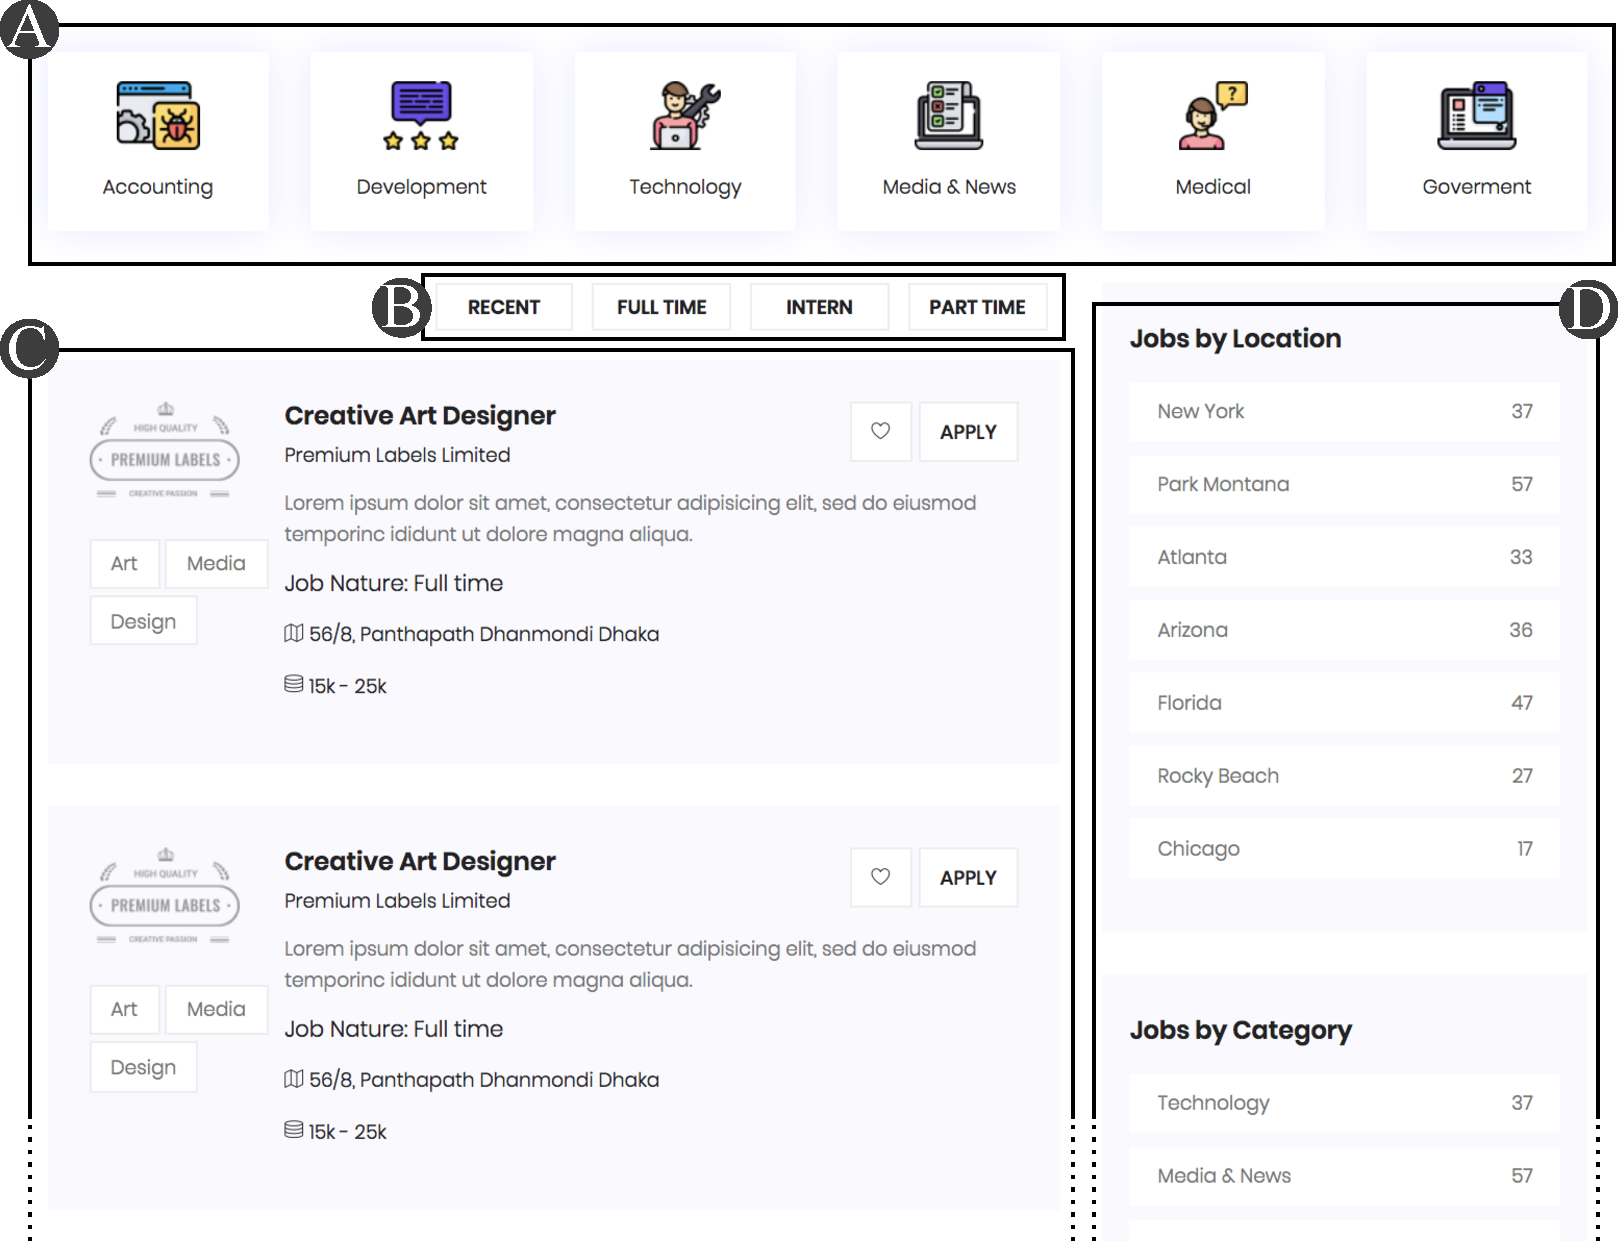
\includegraphics[width=0.8\textwidth]{maintainability/figures/motivating-example}
    \caption{An example of a web UI mockup.}
    \label{fig:motivating-example}
\end{figure} 


However, the process of creating reusable components is rather time consuming, 
requiring manual effort~\cite{thinking:in:components}.
When analyzing repetitions in a mockup
to construct components in one of the modern UI frameworks,
developers often face the following challenges:
\begin{itemize}[leftmargin=*]
	\item They need to visually glance at the mockup and manually identify the patterns in the UI
	that can be potentially refactored to create a reusable component.
	For instance, for group \circled{A}, they need to find all patterns in 
	the page that represents components similar to the elements inside
	group \circled{A}.
	The repetition might be spread across the web page,
	making the identification more challenging.
	The developer has to repeat this same process for other groups of components on the page, which quickly becomes a time consuming manual effort. 
	Note that, this identification is not possible by only using existing code clone detection tools
	that support \html code as input (e.g., \nicad~\cite{Roy:2008:NiCad}),
	due to several reasons:
	
	\begin{enumerate}[leftmargin=*]
		\item These tools leave out the visual appearance of the elements 
	and only work at the source code level, which is sub-optimal since there are several \textit{inherent patterns}
	in \html which do not necessarily represent a UI component. 
	For example, \html tables are declared using a \code{<table>} tag
	followed by a series of other tags, e.g., 
	\code{<thead>}, \code{<tbody>}, 
	\code{<colgroup>},
	\code{<tr>}, and \code{<td>},
	nested in a predefined hierarchy.
	The clone detector might mark all tables on the page for extraction, even if they do not visually constitute a reusable component in the UI.
	The same happens for several other elements, such as (un)ordered, description, and drop-down lists.	

	\item Clone detectors need to be configured properly in order to yield desirable clones.
	There is usually a large list of parameters and thresholds to tune,
	and finding an optimal configuration is a laborious task~\cite{Wang:2013:SearchingForBetterConfigs}.
	
	\item Clone detectors are not aware of the ultimate reason for detecting clones,
	e.g., there is no configuration that can force them to only identify clones that can be unified into a component template. 

	\end{enumerate}
		
	\item The developer also needs to \textit{unify} the patterns
	to construct a reusable component in a UI framework.
	This process needs careful investigation of repeated \html,
	to identify how elements can be unified into one representative component,
	and which elements can be \textit{parameterized} when there are differences.
	For example, in group \circled{A}, a developer would examine each button in the group, and determine which parts are repeated between the buttons, and which part is variable (e.g., the button icon and its label).
	The constructed component should resemble the exact hierarchy of the original repeated elements,
	or else the output of the resulting UI might differ from the original one.
	
	 
	\item Moreover, to use the constructed component,
	the developer has to \textit{instantiate} it
	in the places where the repeated elements originally appeared,
	with the appropriate parameters (e.g., original texts or images)
	to preserve the output of the mockup.
	For example, in group \circled{A}, the developer needs to refactor the original code and replace every occurrence of a button with a call to the button component, passing along arguments for the button label and its image.
\end{itemize}

To the best of our knowledge, there has been no techniques 
available to address the aforementioned issues and 
support developers in the generation of components.







% !TEX root =  paper.tex


\section{Proposed Approach}
\label{section:approach}


\Cref{fig:approach-diagram} shows an overview of our proposed approach
to automatically generate modularized reusable UI components
from mockups.
The approach begins by retrieving the DOM of the web app's mockup. 
Next, a visual abstraction is performed to generate a normalized and abstract representation of the web app's UI layout.
This transforms the mockup into a set of {\VizElem}s ({\VE}s) on which further analysis is conducted. 
The approach then performs a dynamic grouping  of {\VizElem}s,
to identify subtrees
which correspond to potential instances of a UI component. 
This grouping is used in the next step, where an unsupervised machine learning technique applied on the 
potential UI component instances identifies UI components.
Finally, the actual code for the UI components is generated by refactoring the original \html code.

\begin{figure}
    \centering
    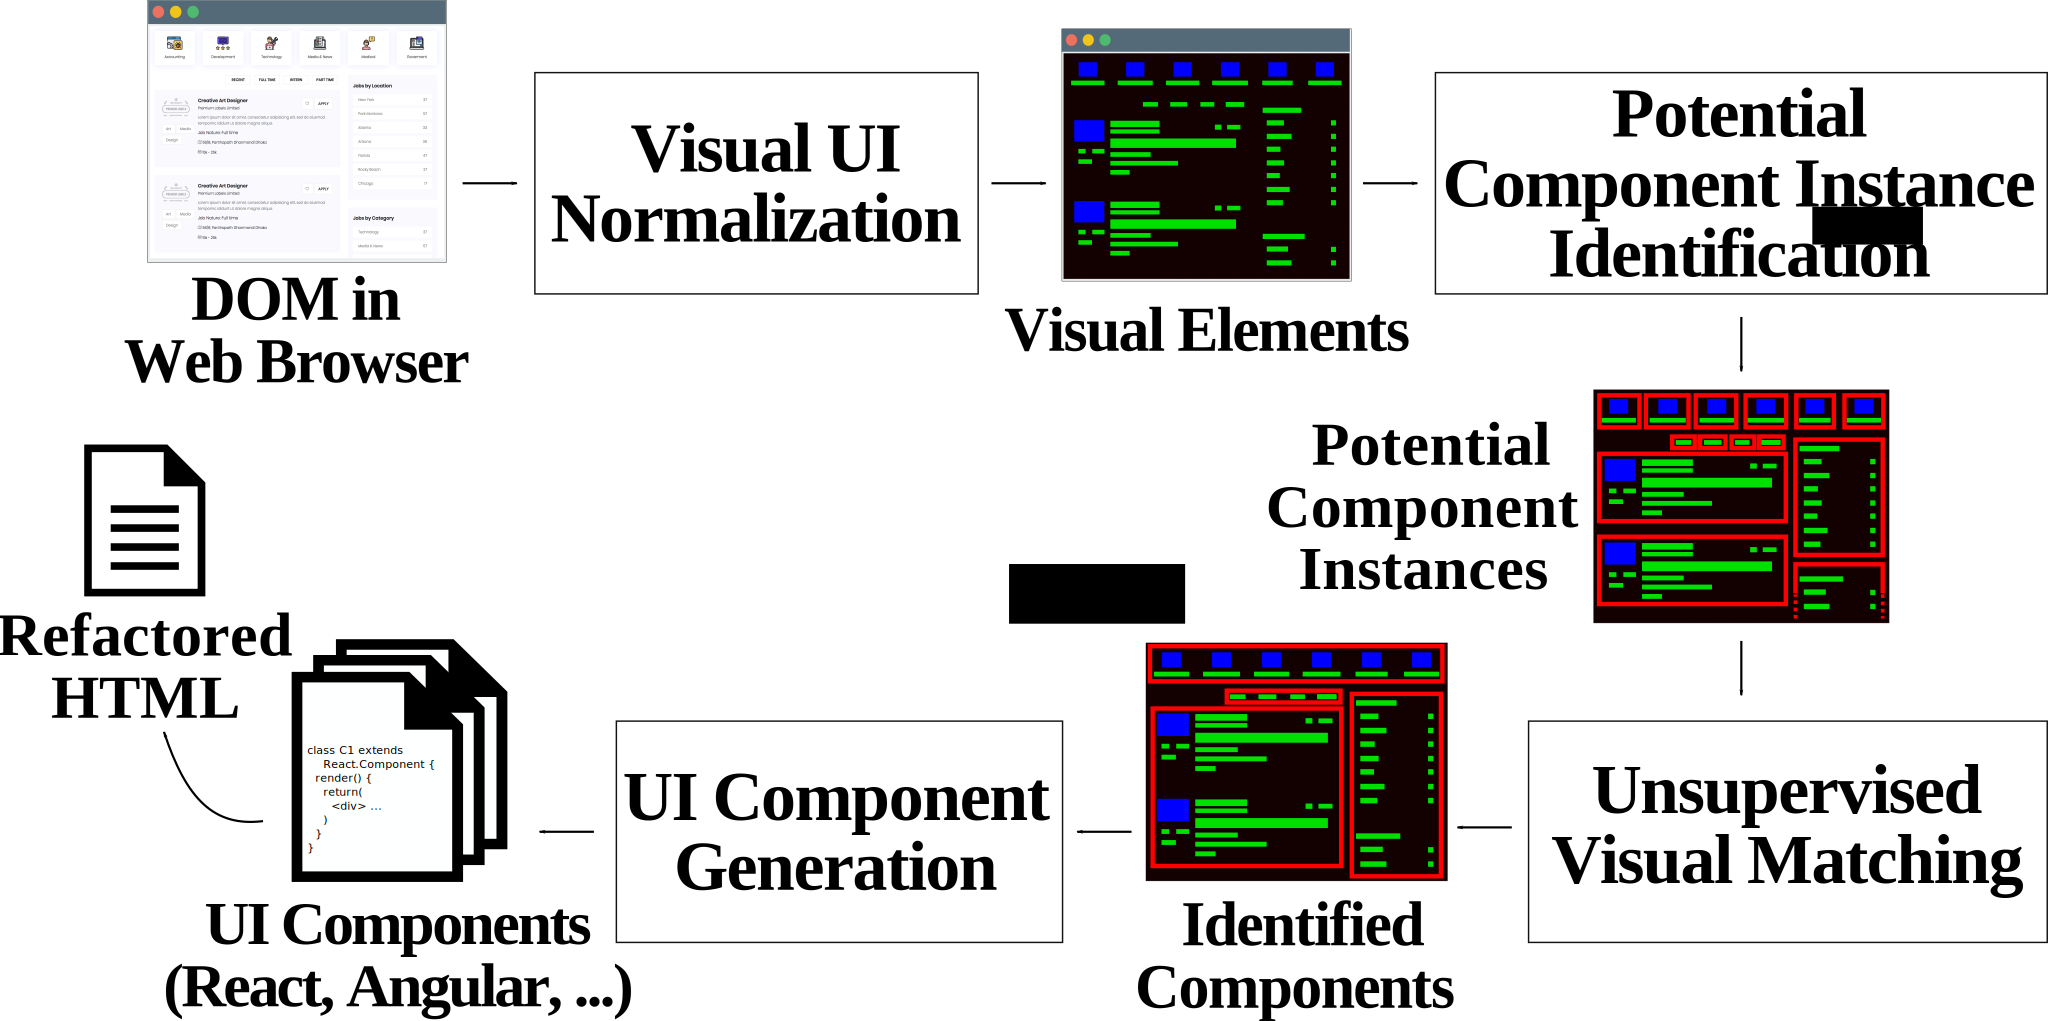
\includegraphics[width=0.75\linewidth]{maintainability/figures/approach-diagram}
    \caption{Overview of the proposed approach.} 
    \label{fig:approach-diagram}
\end{figure} 


In the following subsections, we describe each step of the proposed approach and illustrate some of their major components and analysis procedures. 

\subsection{Definitions}
Before we proceed to describe the details of the proposed approach, we begin by declaring a few important definitions that are used throughout the chapter.
\begin{defn}[\textbf{UI Component}]
A UI component $c_E=\langle n, N \rangle$ 
for a repeated group of UI element trees $E$ in a web application
is a tree structure rooted at $n \in N$, where $N= T \cup P$ is a set of abstract user interface elements.
The component includes the \emph{template} $T$ and the \emph{placeholders} $P$.
The template of the UI component denotes the nodes which do not change wherever the component is used (i.e., \emph{instantiated}),
while the placeholders captures the changed nodes, whether partially or fully changed, as explained in \Cref{sec:ui-comp-gen}.
\end{defn} 
In this chapter, we use the terms \textit{UI component} and \textit{component} interchangeably.


\begin{defn}[\textbf{Component Instance}]
A component instance $i=\langle c_E, f \rangle$ is a concrete and specific instantiation of a UI component $c_E$. 
Component instances share the template part with other instances of the same component, 
but differ in the placeholder parts.
The function $f: P \rightarrow V$ assigns values $v \in V$ to the placeholders $p \in P$ of $c_E$.
\end{defn}

\begin{defn}[\textbf{Potential Instance}]
A potential instance is a subtree of the \dom 
constructed for a web application's user interface,
representing a concrete UI element tree 
that is \emph{likely} to form a component instance, but may not be so. 
\end{defn}

Potential instances are processed at multiple stages of the proposed approach 
until they are either discarded or associated with a component.


\subsection{Visual UI Normalization}
In the first step of the approach, we take as input the DOM of the mockup after it is loaded and rendered in a browser,
and perform a \emph{visual normalization} that transforms the DOM into a set of \emph{{\VizElem}s}.
The goal of this step is to normalize the visual presentation of a web user interface into a set of abstract elements 
that signify the salient features of the page from a visual perspective, which may represent potential component instances.
The intuition behind this is that normalization and abstraction can be helpful to achieve our goal of detecting reusable patterns, since the exact and minute details are less relevant when identifying repeated regions of a web page. 
Furthermore, component instances are generally different from each other in some aspects, while they still have similar overall visual appearance. 
This normalization step enables obtaining a big picture to identify these potential similarities.% between different instances.

The visual normalization is achieved as follows.
First, we extract from the DOM a set of nodes that represent visual content of the UI, and we refer to each of these as \emph{{\VizElem}s}.
We define two main types of {\VizElem}s: textual and graphical (image).
The extraction of text content is achieved by traversing text nodes of the DOM. More specifically:
%\begin{align}
%VE_{T} \coloneqq \{ node \in DOM \!\, : \, & node.type=\code{\#TEXT} \nonumber \\
%                       \lor \, & node.tag=\code{input} \}
%\end{align}
\begin{align}
\Gamma_{T} \coloneqq \{ E(node) : \ & node \in DOM_R \!\, 			\land \,  & node.hasTextContent \}
\end{align}
where $\Gamma_{T}$ is the set of all visual elements that represent text in the UI, $DOM_R$ is the rendered DOM in the web browser, and $E(node)$ maps the node to the corresponding element. 
%\davood{visual element?}
The predicate $hasTextContent$ examines whether there is a text associated with the node, 
and covers two possibilities: non-empty nodes of type \code{\#TEXT}, representing string literals in $DOM_R$, 
and nodes of \code{input} elements that have an associated text value (e.g., buttons or lists).
Subsequently, we perform another extraction for image content. We define this as follows:

%\begin{align}
%VE_{I} \coloneqq \{ & node \in DOM \!\, : \, node.tag=\code{img} \nonumber \\
%                       \lor \, & node.hasBackgroundImage \}
%\end{align}
\begin{align}
\Gamma_{I} \coloneqq \{ E(node) : \ & node \in DOM_R \!\, 		\land \, & node.hasImageContent \}
\end{align}
where $\Gamma_{I}$ is the set of all visual elements that represent images. As in the previous case, the predicate $hasImageContent$ examines if there is an image associated with the node. This again has two possibilities: nodes of \code{<img>} elements and non-img nodes with a non-null background image attribute. 

Subsequently, we use the set of all {\VizElem}s to construct the normalized UI: 
\begin{align}
\mathrm{UI}_N = V\!\left( \Gamma_I \cup \Gamma_T \right)
\end{align}
where $\mathrm{UI}_N$ is the resultant normalized UI and $V$ is a visual projection operation that generates an image from the union of visual elements. This is achieved as follows. First, we begin by collecting the final \emph{computed} properties of each element,
when rendered in the web browser. These properties represent the final state of elements after the propagation of all changes and events. The properties we collect are the size, location, and z-orders of these elements. Next, we assign different colors to each class of {\VizElem}s.
We assign green for elements in $\Gamma_{T}$, and blue for elements in $\Gamma_{I}$.
While any arbitrary colors could have been chosen, we chose these two colors in order to facilitate faster visual analysis in subsequent steps, since these two  are typically represented in separate color channels.
\Cref{fig:example-normalization} illustrates an example of the output generated from this visual normalization step.
As can be observed, the minute details of the page are abstracted away while the main and essential structure of the UI is accentuated. 

\begin{figure}
    \centering
    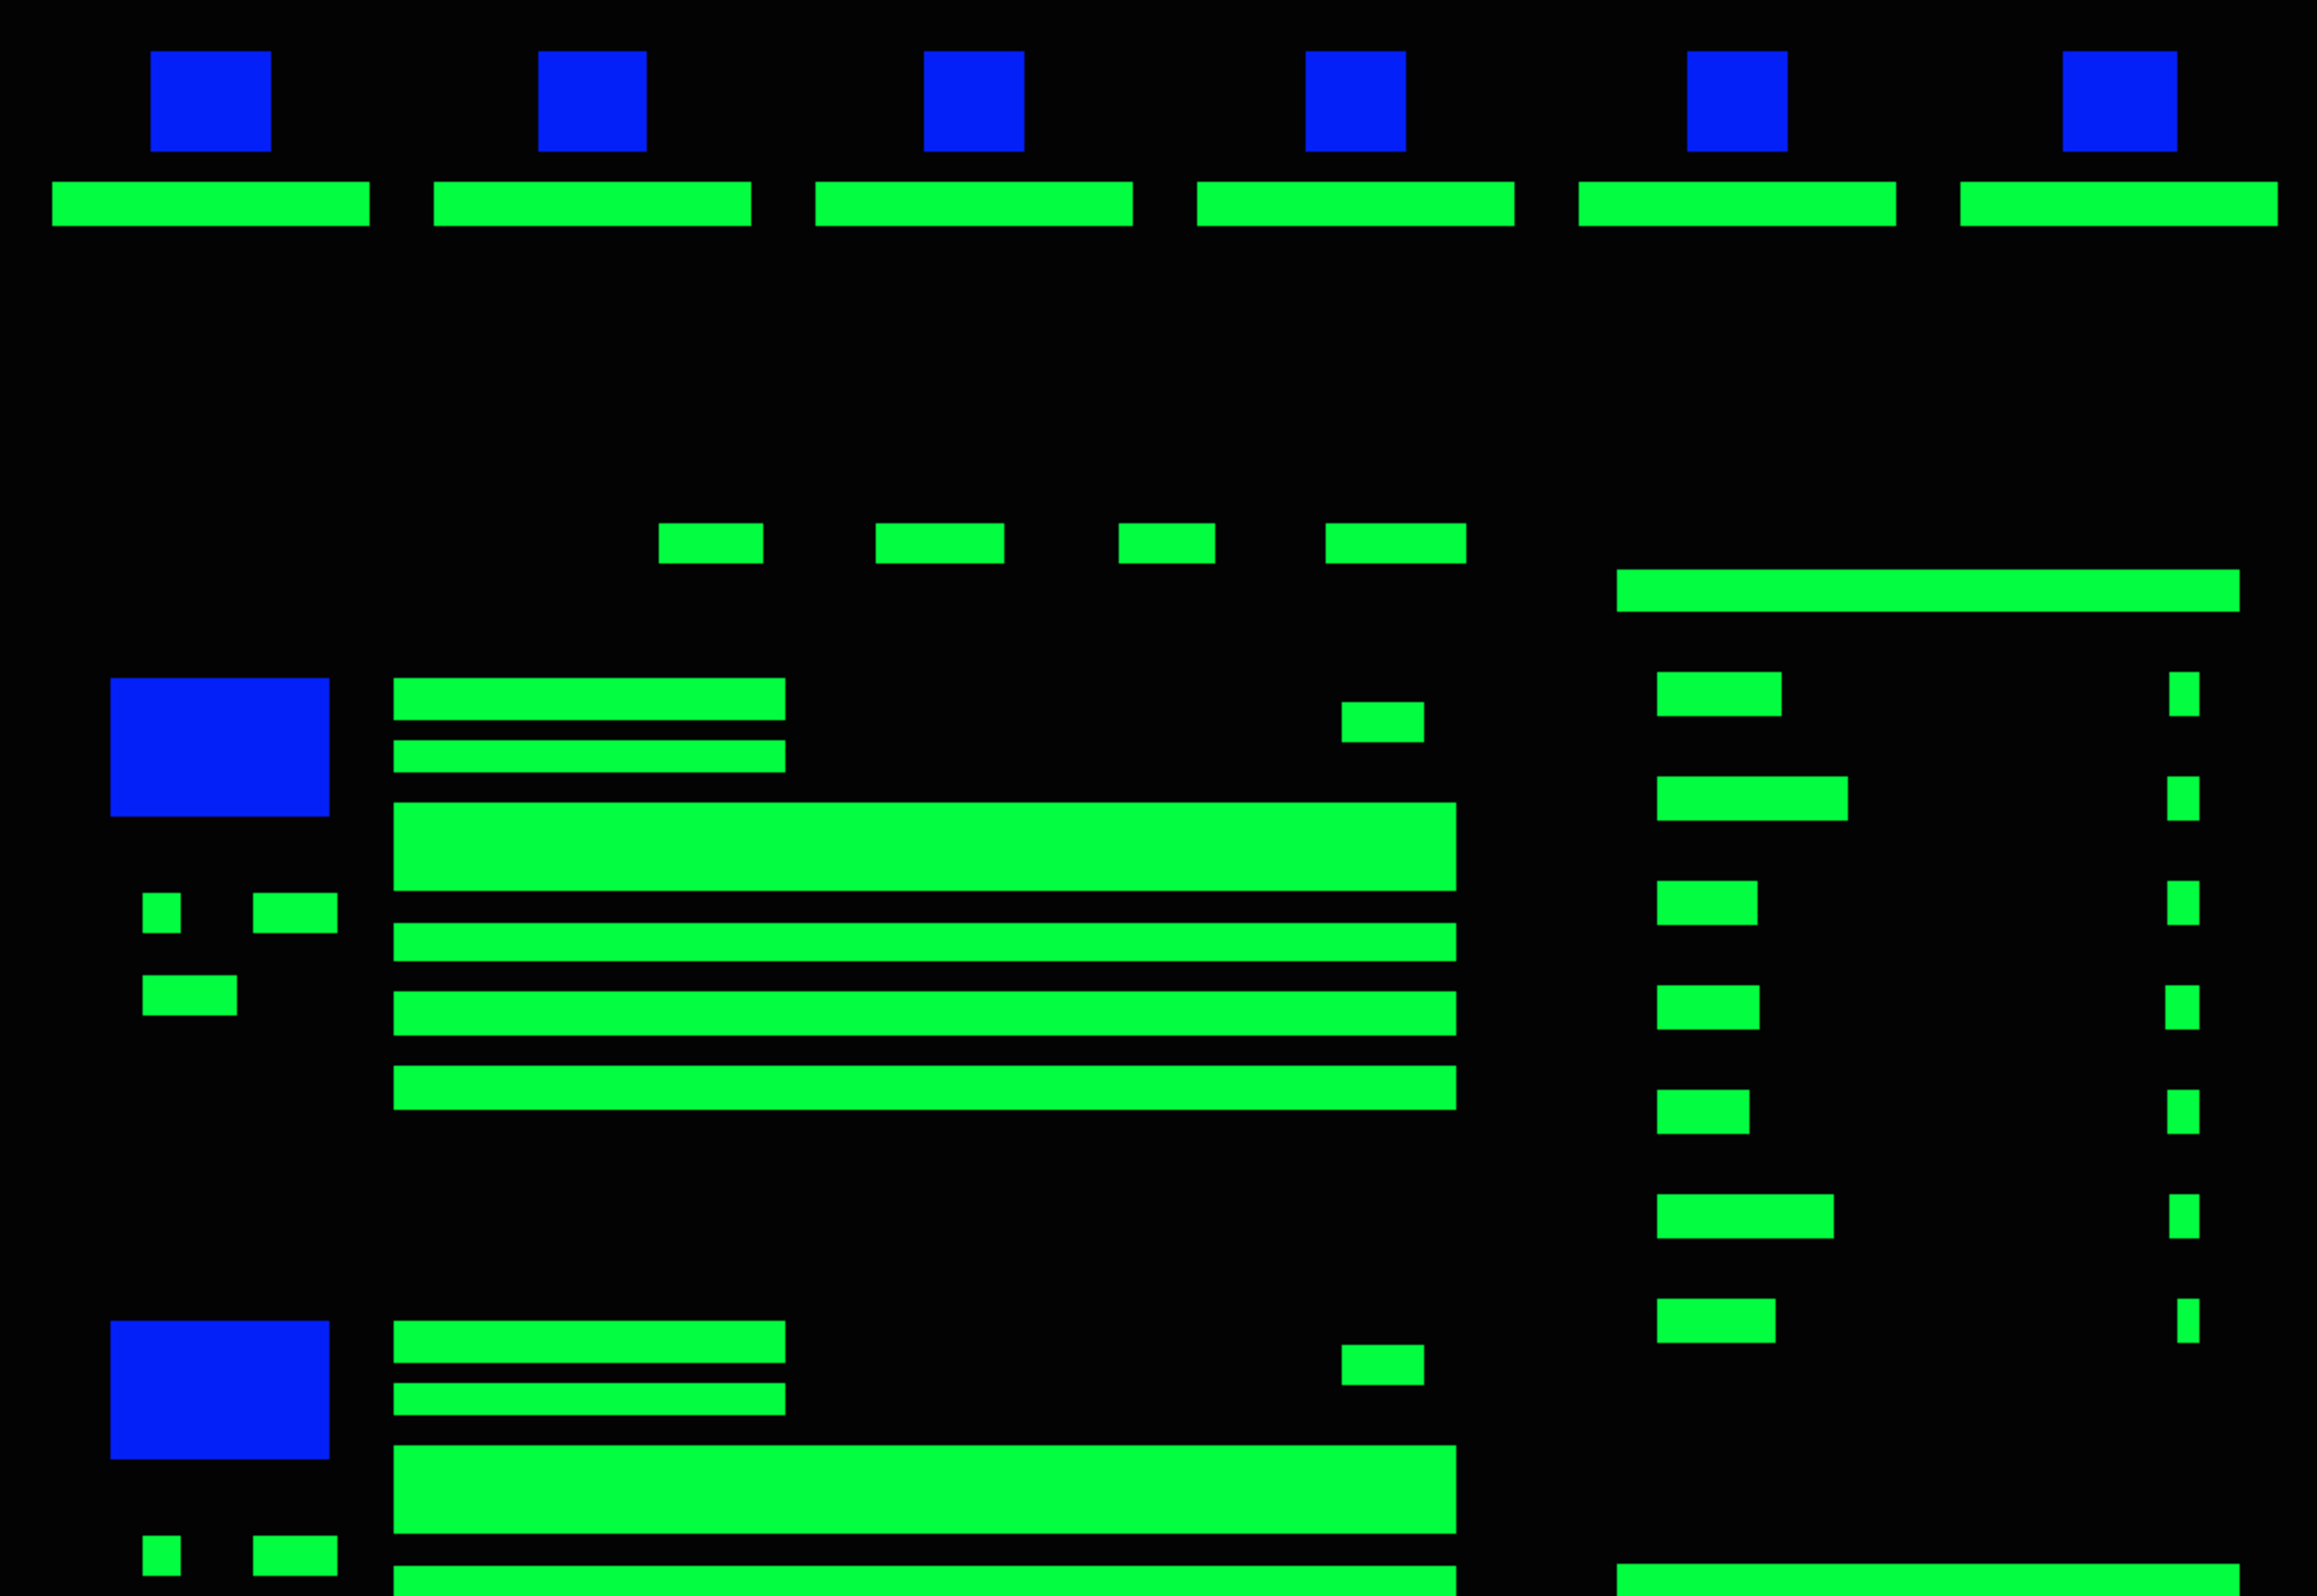
\includegraphics[height=3.5cm,width=0.40\textwidth, clip, trim={0 0cm 0 0cm}]{maintainability/figures/example-normalization}
    \caption{The result of the visual UI normalization stage (as applied to the motivating example of \Cref{fig:motivating-example}). Best viewed on a color display.}
    \label{fig:example-normalization}
\end{figure} 

\subsection{Potential Instance Identification}
The result of the previous step consists of only a set of {\VizElem}s.
These {\VizElem}s on their own do not \emph{necessarily} represent reusable repetitive UI patterns. 
The goal of this step is to transform the set of individual {\VizElem}s into a set of \emph{potential} reusable UI component instances.
A potential instance is a region of the UI that has been determined to be likely repeated somewhere else in the UI. That is, it is 
a region where, using all of the aforementioned steps, the 
initial analysis have indicated that this instance would likely be a good candidate to be combined with other repetitions and refactored 
into a single component. These potential component instances will be further checked and analyzed in the subsequent steps in order to generate a final set of components.

Identifying potential component instances can be an intricate decision since there are multiple levels of hierarchy that can be considered.
For example, consider group \circled{A} in \Cref{fig:motivating-example}.
Notice how the icons in that group would constitute repeated elements.
The same is true for the text labels under the icons.
Yet another repetition pattern is taking the icon and text as one component that is repeated multiple times. 
Accordingly, in order to identify potential component instances, we propose an approach that aims to maximize two complementary aspects, namely, 
the number of repetitions of a component,
and the amount of repetitions encapsulated \emph{within} each component instance (i.e.,~repetitions of the \emph{same} potential instances).
We refer to this combination of aspects as the \emph{modularization potential}, where a high value of modularization potential indicates a potentially more reusable UI component.
Our goal is therefore to utilize this modularization potential to optimize a set of potential instances, $\Psi$:
% capture these aspects in a quantitative manner and optimize for the \emph{maximal modularization component set}, $MMCS$:
%\begin{equation} \label{eqn:MMCS}
%\Psi \coloneqq \argmax_{C} \prod_{c_i \in C} \big\lvert \{VE_T \cup VE_I  : VE_T, VE_I \in c_i\} \big\rvert
%\end{equation}
\begin{equation} \label{eqn:MMCS}
\Psi \coloneqq \argmax_{C} \prod_{c_i \in C} \big\lvert \{c_i(\gamma_T, \gamma_I) : \gamma_T, \gamma_I \subset \mathrm{UI}_N\} \big\rvert
\end{equation}
where $C$ is the set of all component instances, $c_i$ is a potential instance, and the optimized function is the modularization potential.
This optimization yields a global optimum set of potential instances between two extremes.
At one end of the spectrum,
each {\VizElem} represents a component of its own.
This yields a sub-optimal component set that has low modularization potential because of a lack of repetitions.
For this case, the modularization potential in \cref{eqn:MMCS} yields a score of 1 since each component encapsulates only a single element.
At the other end of the spectrum,
one might theoretically consider the \emph{entire} collection of {\VizElem}s to represent a single component that is repeated only once.
This results in a score equal to $N$, the number of total {\VizElem}s, in \cref{eqn:MMCS}.
$\Psi$, on the other hand, represents a global optimum between the aforementioned two extremes. $\Psi$ captures a set of potential component instances that aims for \emph{both} a large number of components, and for an instance that in itself has a large number of UI repetitions.
The subsequent steps of the approach will therefore only use $\Psi$ for further analyses and final generation of components.

We now describe the implementation for generating $\Psi$. \Cref{fig:instance-potential-identification} shows an illustration of this process.
First, we obtain DOM locators (e.g., {\xpath} expressions) for each of the {\VizElem}s. Next, starting from these locators as leaf nodes, we iteratively build a tree from the bottom up (as shown in \Cref{fig:instance-potential-identification}), adding the DOM parent of every tree node with each iteration.
At each iteration, we calculate the modularizaton potential of \cref{eqn:MMCS}, with every node's subtree representing a potential instance $c_i$. 
The potential instances are illustrated using the red outlines in \Cref{fig:instance-potential-identification}. Note how at the very first iteration, each potential instance is simply the \VizElem~itself. In the next iteration, the potential instances grow larger to include more {\VizElem}s as shown by the larger red outlines at iteration 1.
Finally, the iteration that yields the maximal modularization is  reported as the $\Psi$ set and passed to the subsequent stage.

\begin{figure}
    \centering
    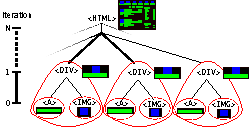
\includegraphics[width=0.9\linewidth]{maintainability/figures/potential-component-identification}
    \caption{Illustration of the potential instance identification stage. Each iteration considers a different group of potential instances before selecting an optimum set.}
    \label{fig:instance-potential-identification}
\end{figure} 

\subsection{Unsupervised Visual Matching}
The output of the previous step is a set of \emph{potential} component instances that maximizes the modularization potential out of many alternative sets of instances.
However, these are only \emph{potential} instances that may or may not actually belong to a component.
In other words, there is still no information as to which subgroup of potential instances do indeed belong together and constitute a reusable component,
versus other potential instances that are simply visual elements that do not represent repetitive reusable components.
In this stage, we process the set of \emph{potential} component instances and reduce it into a final set of components. 

In order to create the final components,
we propose an approach that visually examines potential instances and combines them into components via unsupervised machine learning.
The intuition behind adopting this approach is that if potential instances match with other potential instances,
the ``potential'' qualifier can be dropped from these instances and they would be recognized as constituting a component together.
In this approach, we use a clustering mechanism to create components in order to facilitate robust matching of potential instances.

We now describe the details of the process. First, we obtain the screenshot image of the {\VizElem}s per potential instance. This results in one image (containing all {\VizElem}s) for each potential instance. Next, for each potential instance image, we extract a feature vector. We compute the feature vector using a \emph{vectorized pixel histogram}, which is a process that captures a summary of the overall content in the instance image. However, unlike typical approaches from the machine vision literature~\cite{lopes2010automatic, liu2010image} where a binning parameter (a parameter for categorizing pixels) is required, we generate the vectorized histogram without requiring this parameter. Instead, due to the nature of visual normalization that we have proposed, only two categories need to be considered: one for text visual elements, and another for image visual elements. Therefore, we finally end up with a feature vector for each potential instance. Subsequently, we compute the cosine distance between each pair $\mathbf{I}_i$, $\mathbf{I}_j$ of potential instances:
\begin{equation} \label{eqn:cosdist}
D_{i,j} = 1 - \frac{\mathbf{I}_i \cdot \mathbf{I}_j}{ \lVert \mathbf{I}_i \rVert \lVert \mathbf{I}_j \rVert }
\end{equation}

Next, we perform an unsupervised clustering process. The selection of an appropriate clustering is of paramount importance due to a couple of challenges. First, the clustering can be challenging due to the wide range of possibilities of arrangements and structures of component instances. In other words, there is potentially a large range of \emph{inter-} and \emph{intra-}component variations. 
This makes it difficult to use hierarchical clustering, for instance, due to its very high sensitivity to outliers and therefore would be a poor choice for handling large component variations, and also due to its high dependence on order of data, which can make it less effective for detecting instances far way from each other. Furthermore, performing a cut on the clustered hierarchies often requires specifying the number of clusters or some other parameter, which can be difficult and brittle to specify. Density-based algorithms (e.g., DBSCAN) would not be effective either, as they would have difficulty handling the \emph{variable} densities present between potential clusters of instances. Accordingly, we opted for a technique that can be flexible enough to correctly identify such variations and be able to better recognize the final components. To do this, we select a method that performs variable-density clustering with a hierarchy of densities \cite{campello2013density}. The hierarchy of variable-densities allows the method to automatically detect stable clusters in a parameter-free fashion. More importantly, the method is built to handle varying-densities, which becomes very important when handling the potentially large range of inter- and intra-component variations.
 
Once the components have been identified through unsupervised visual matching,
we extract the corresponding locator in the DOM (e.g., {\xpath}s) per instance.
The final result is a superset of component instance locator sets.
This superset is passed on to the next step in order to combine the component instances into final components.


\subsection{UI Component Generation}
\label{sec:ui-comp-gen}
% !TEX root =  paper.tex
We propose an algorithm that unifies the UI component instances 
identified in the previous steps
into a component
implemented using a web framework (e.g., \react, \angular, \html Web Components~\cite{MDN:2017:WebComponents}).
However, instead of directly generating the framework-specific code for components,
we opt for constructing an \textit{intermediate model}
that effectively represents components at a higher level of abstraction.
This allows building different \textit{translation strategies}
for generating the actual code 
for different frameworks from the same model,
with the added benefit of remaining agnostic 
to the specific details of a particular framework. 
Our implementation supports the \react~\cite{React} translation strategy,
 which is the preferred framework for a significant number of developers in practice~\cite{StateOfJS:WebPlatformTests, StackOverflow:2017:Survey}.
We first define the terms used in this step.

\begin{defn}[\textbf{\mappedset}]
	\label{definition:mapped-nodes-set}
	Let $T = \{t_1 \ldots t_n\}$ be the list of \dom subtrees for $n$ instances
	of a UI component identified by the previous phases of the approach.
	%These subtrees are rooted at the \dom nodes located by the {\xpath}s 
	%returned by the previous phase.
    A set $D = \{d_1 \in t_1, d_2 \in t_2\ldots d_n \in t_n\}$ of \dom nodes corresponding to $T$
	is a \mappedset,
	when every pair $(d_i, d_j)$ of \dom nodes 
	belonging to $D$ are \textbf{mapping}.
\end{defn}

\begin{defn}[\textbf{Mapping}]
	Two \dom nodes $d_i$ and $d_j$
	are mapping (denoted as $d_i \leftrightsquigarrow d_j$) when:
	\begin{itemize}[leftmargin=*]
	\item Both $d_i$ and $d_j$ are root nodes of their trees, or 
	\item $d_i$ and $d_j$ are not root nodes, and
	\begin{itemize}[leftmargin=*]
		\item $d_i.parent.tag = d_j.parent.tag$, and
		\item $d_i.parent \leftrightsquigarrow d_j.parent$, and
		\item $d_i$ and $d_j$ have the same child index 
		(e.g., they are both the first child of their parents).
	\end{itemize}

	\end{itemize}
\end{defn}

\begin{defn}[\textbf{\model}]
	The \model is a rooted, ordered tree
	in which each node corresponds to a \mappedset.
	The hierarchy of this tree follows the mapping \dom nodes' hierarchy.
\end{defn}


\header{Example} \Cref{fig:intermediate-model-sample-dom-subtrees}(a) 
depicts the \html code snippets 
corresponding to two identified UI component instances.
%(the visual output is omitted due to space limitations).
The corresponding \dom subtrees,
and the constructed \model for these subtrees 
are respectively shown in \Cref{fig:intermediate-model-sample-dom-subtrees}(b) and (c).
The connected \dom nodes with dotted arrows form {\mappedset}s.
Notice that non-mapping \dom nodes do not form a node in the intermediate model.
This model can be translated to a \react-like component
similar to what is shown in \Cref{fig:intermediate-model-sample-dom-subtrees}(d).
Finally, the generated component is instantiated two times in the refactored \html code
to replace the originally-repeated \dom nodes.
The calls to the component can look like what is shown in \Cref{fig:intermediate-model-sample-dom-subtrees}(e).

\begin{figure}
    \centering
    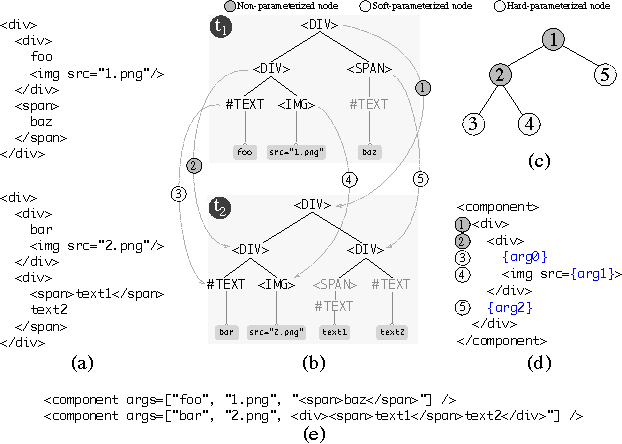
\includegraphics[width=0.70\textwidth]{maintainability/figures/intermediate-model}
    \caption{
    	(a) Initial \html code fragments.
     	(b) Corresponding \dom subtrees.
     	(c) The constructed \model.
     	(d) The final generated UI component.
     	(e) The \textit{calls} to the generated UI component.}
    \label{fig:intermediate-model-sample-dom-subtrees}
\end{figure} 

When generating the actual framework code,
each model node results into a \dom node in the framework component
(as depicted in \Cref{fig:intermediate-model-sample-dom-subtrees}(d)),
which essentially \textit{unify} the nodes in the \mappedset
to remove duplication.
There are three possibilities for framework component \dom nodes:

\begin{itemize}[leftmargin=*]

	\item When all pairs of \dom nodes in a \mappedset have the same tag and identical attribute values,
	they can be unified in one \dom node of the same tag.
	For example, the two \code{<div>} nodes in \Cref{fig:intermediate-model-sample-dom-subtrees}
	corresponding to model node \circled{1}
	form a \code{<div>} node in the component.
	
	\item A pair of \dom nodes in a \mappedset which have different tag names
	cannot be unified into one \dom node in the component
	(e.g., \code{<span>} and \code{<div>}
	corresponding to model node \circled{5} in \Cref{fig:intermediate-model-sample-dom-subtrees}).
	Similar is two text nodes with different content
	(e.g., the \code{foo} and \code{bar} corresponding to the model node \circled{3} in \Cref{fig:intermediate-model-sample-dom-subtrees}).
	In such cases, the \dom nodes (and the whole subtree rooted at them) should be \textit{hard-parameterized} in the resulting component,
	i.e., a \textit{placeholder} should be created.
	The original parameterized \dom nodes are later passed as \textit{arguments} when instantiating the component
	to recreate the original \dom hierarchy.
	
	\item A pair of \dom nodes in a \mappedset that have the same tag name but
	different values for one of their attributes
	might be unifiable into a \dom node 
	via \textit{soft parameterization},
	where the differing attribute values are parameterized
	(e.g., the \code{<img>} tags corresponding to model node \circled{4}
	in \Cref{fig:intermediate-model-sample-dom-subtrees},
	with parameterized \code{src} attribute values).
	This can be done only if the used framework supports parameterizing attribute values.
	Otherwise, the parameterization should be done as if it was a hard parameterization.

\end{itemize}

\header{The intermediate model construction and refactoring algorithm}
The inputs of \Cref{algorithm:refactoring} are the original mockup \html, 
the list of component instance \dom subtrees,
and the translation strategy.
The output is the refactored \html wherein duplication is removed using the UI components.

\begin{algorithm}
	\fontsize{7.5pt}{9pt}\selectfont
	%\linespread{1}\selectfont
	\caption{\model Generation}
	\label{algorithm:refactoring}
	\input{maintainability/algorithm-component-generation}
\end{algorithm}

\Cref{algorithm:refactoring} starts by constructing an empty model (\cref{algoline:ui-component-empty-model}),
and an exclusion list (\code{coveredNodes} in \cref{algoline:ui-component-covered-nodes-init})
that contains the original \dom nodes of the component instances which are already covered by the algorithm
(e.g., a model node has been created for them),
so that they are skipped in future iterations.
To construct the intermediate model,
the algorithm chooses the \dom subtree of one of the component instances
(i.e., the \emph{template subtree}) to follow its hierarchy.
The template subtree is the one with the smallest number of \dom nodes,
chosen in \cref{algoline:ui-component-template-tree}.
This is because the intermediate model cannot have more  \dom nodes than the smallest subtree,
as it resembles the \textit{intersection} of the component instances' \dom subtrees.
The algorithm loops over all the uncovered template subtree's \dom nodes,
following the subtree's breadth-first traversal order
(lines~\ref{algoline:ui-component-main-loop-start} to \ref{algoline:ui-component-main-loop-end}).
Each template \dom node 
is compared to other \dom nodes of its \mappedset (identified according to \Cref{definition:mapped-nodes-set}
in \cref{algoline:ui-component-mapped-nodes-set})
using the \code{compare()} function (\cref{algoline:ui-component-compare}),
which returns the type of parameterization needed to unify two given \dom nodes,
and \code{NULL} if no parameterization is needed.
Note that, even if one node in a \mappedset should be parameterized 
when compared to the template \dom node, 
the resulting model node will be either hard- or soft-parameterized,
thus comparing other nodes of \mappedset is not required
(\cref{algoline:ui-component-break}).

The intuition behind comparing nodes in the breadth-first order is that,
across the component instances' \dom subtrees, it is more likely that the the inner nodes (which define the structure of the final UI component) 
are similar,
while the leaf nodes (texts, images) are more probable to differ.
%In addition, when a set of mapping inner nodes should be hard-parameterized,
%all the subtrees rooted at the mapping nodes should be parameterized,
%meaning that there will be no need to assess them in the future.
The inner nodes are thus compared before leaves,
also facilitating the identification of \mappedset based on \Cref{definition:mapped-nodes-set},
as the nodes' child indices follow the BFS traversal order. 
%\davood{I think DFS would be also possible}

The algorithm then continues to add a model node for each \mappedset
(lines~\ref{algoline:ui-component-add-model-nodes-start} to \ref{algoline:ui-component-add-model-nodes-end}).
First, the model node that has been created for the template \dom node's parent 
(in the previous runs of the loop) is retrieved from the model (\cref{algoline:ui-component-add-model-nodes-start}),
to which the new model nodes will be added as children.
This effectively allows the model to preserve the original hierarchy of the instances' \dom subtrees.
If the model is empty, the new model node will form the model's root.
The subsequent lines of the algorithm add the new model node
based on the parameterization type.
In each step, the \dom nodes in the \mappedset for which a model node is created
are added to the \code{coveredNodes} to be skipped in the next iterations.
As mentioned, in case of a hard-parameterized model node,
all the \dom nodes belonging to the subtrees rooted under the corresponding mapping \dom nodes
should be marked to be skipped (e.g., node \circled{5} in \Cref{fig:intermediate-model-sample-dom-subtrees}).

Finally, the actual refactoring is conducted using the constructed \model (\cref{algoline:ui-component-refactor}).
The details of the refactoring are built-in the translation strategy,
which can be implemented virtually for any UI framework of interest.





\header{Implementation}
\label{section:implementation}

We implemented the proposed approach in a tool called \toolname~\cite{tool-and-data} (short for \textbf{Vis}ual \textbf{Mod}ularizer). 
\toolname is implemented in Java and Python~3. We use the Selenium web driver to view the mockup and extract DOM trees and their relevant computed properties. 
For clustering, we use the implementation provided by Campello et. al.~\cite{campello2013density} 
and the \code{numpy}~\cite{walt2011numpy} library for mathematical and numerical functions. 




 

% !TEX root =  paper.tex

\section{Evaluation}
\label{section:evaluation}

To evaluate \toolname, we conducted 
qualitative and quantitative studies 
aiming at answering the following research questions:

\begin{enumerate}[label=\textbf{RQ\arabic*},leftmargin=*]

	\item Are the refactorings by \toolname's component generation correct?

	\item How effective is \toolname 
	in identifying UI components compared to manual examination by web developers?
	
	\item How much code reusability can be achieved through the proposed refactorings? 
	
\end{enumerate}

In the following subsections, we discuss the details of the experiments
that we designed to answer each research question,
together with the results.

\subsection{RQ1: Correctness of Component Generation Refactorings}

\subsubsection{Study Design}

For the proposed componentization applied on \html to be safe, 
the main criterion is that the original and the refactored {\html}s 
must result into the same \dom tree landed into the users' web browsers.
Consequently, to devise a technique that can automatically assess 
the safety of the applied transformations,
we relied on the equivalence of the \dom subtrees 
rendered in the web browser,
before and after refactoring.
If the \dom trees are the same, given that our refactorings do not change
any \css style rules, the resulting presentation semantics of the \html files remain intact. 

To automate this process, we serialized the final \dom trees rendered in the browser
to the pretty-printed \html code and compared them pre- and post-refactoring.
This allows a fast comparison of the structure of the \dom trees.
We normalized the \dom trees by removing text nodes which are empty or contain only white spaces.
This is done because \react interprets these nodes differently~\cite{React:WhitespaceIssue, React:JSXWhiteSpaces} compared to the standard \html specifications.

\subsubsection{Results and Discussion}
Using the aforementioned technique, 
we compared the \dom subtrees of the UI component instances
before and after refactoring for the \totalNumberOfComponentInstances UI component instances 
(i.e., \numberOfComponents UI components) identified by \toolname.
The tests has passed for all subjects,
indicating that the refactorings introduced by component generation do 
preserve the \dom trees,
and as a result, the transformations are safe to apply.


\subsection{RQ2: UI Component Identification}

\subsubsection{Study Design} 
\label{sec:study-design}

We asked independent expert web developers to participate in a qualitative study,
with the goal of understanding what they would identify as
being a component pattern in a web UI. 
With this study, we aim at evaluating the (dis)agreement between the proposed approach and expert developers in terms of identifying the UI components.



\header{Subject Systems}
We searched the Internet to find mockups suitable for this study
(using keywords like ``web mockups'', ``web templates'', ``front-end templates'').
Our selection criteria for choosing mockups were:

\begin{itemize}[leftmargin=*]
	\item They should be non-trivial, both visually 
	and code-wise (i.e., \html and \css).
	Note in \Cref{table:mockup-complexity} that
	the mockups are indeed complex,
	in terms of the number of \dom nodes and \css code size.
		
\item The number of subjects should be small and manageable enough	
	so that we can ask participants to highlight potential components 
	in \emph{all} of them,
	without causing too much burden, mental fatigue, or boredom on them
	which can negatively distort the study.

	\item They should only represent the UI front-end,
	i.e., without back-end or front-end business logic or functionalities.
\end{itemize}

Based on these criteria we chose \numberOfTemplates mockups for our evaluation. We use the same mockups in all the evaluation experiments.
\Cref{table:mockup-complexity} shows descriptive statistics
for them.

\begin{table}
	\caption{Subjects' descriptive statics}
	\centering
	%\fontsize{8pt}{9.2pt}\selectfont
	%\setlength\tabcolsep{2px}
	\begin{threeparttable}
		\bgroup
		%\def\arraystretch{1.2}
		\begin{tabular}{c r r r}
			\toprule
			\textbf{Subject\#} & \textbf{Body size (KB)} & \textbf{\#\dom nodes} & \textbf{\css size (KB)\tnote\textdagger} \\ \toprule
			        1          & 18                       & 754                   & 323                                      \\
			        2          & 20                       & 915                   & 279                                      \\
			        3          & 33                       & 1,990                 & 350                                      \\
			        4          & 24                       & 1,226                 & 330                                      \\
			        5          & 49                       & 1,065                 & 254                                      \\ \bottomrule
		\end{tabular}
		\egroup
		\begin{tablenotes}
			\item[\textdagger] Some mockups use \css frameworks (e.g., Bootstrap).
			This corresponds to the total \css size, including the frameworks.
		\end{tablenotes}
	\end{threeparttable}
	\label{table:mockup-complexity}
\end{table}



\header{Participants} 
We emailed developers who have worked in local businesses or research labs
and asked them to voluntarily participate in our study.
We attached a zip package containing our subject systems 
together with a link to a post-study questionnaire aimed at collecting information about the participants' demographics
(e.g., number of years of experience in software engineering in general and in web development in particular,
and their self-assessment on web application development skills).
We asked them to manually highlight repetitions on the UI of each subject (by drawing a rectangle on each repetition) and send the results back to us.

Accordingly, we emailed 10 developers and informed them of the study, and asked them to also pass it on to their contacts. We received responses from a total of \numberOfParticipants developers.
\Cref{table:participants-demographics} shows participants'  demographic information.
As it is shown, all the participants were quite experienced in web development,
as measured by the years of software and web development experience
and their own self assessment.

\begin{table}[b]
	\caption{Demographics of the Participants}
	\centering
	%\fontsize{8pt}{9.2pt}\selectfont
	%\setlength\tabcolsep{2px}
	\begin{threeparttable}
		\bgroup
		%\def\arraystretch{1.2}
		\begin{tabular}{c c c c}
			\toprule
			\multirow{2}{*}{\textbf{Participant\#}} & \textbf{SW dev.}   & \textbf{Web dev.}  & \textbf{Web dev. self assessment} \\
			                                        & \textbf{(\#Years)} & \textbf{(\#Years)} & \textbf{(1--5, 5=Highly Expert)}  \\ \toprule
			                   1                    & 10                 & 5                  & 4                                 \\
			                   2                    & 8                  & 2                  & 4                                 \\
			                   3                    & 3                  & 3                  & 4                                 \\
			                   4                    & 11                 & 3                  & 3                                 \\
			                   5                    & 9                  & 8                  & 5                                 \\ \bottomrule
		\end{tabular}
		\egroup
	\end{threeparttable}
	\label{table:participants-demographics}
\end{table}

\header{Comparison with Developers}
For each subject, we compared the components highlighted by the experts 
with those components that \toolname automatically identified as UI components.
In particular, when more than half of the experts
highlighted a pattern on the mockup as repeated, 
we assume the majority is correct and consider it as a UI component  
that our technique should be able to identify.
The performance of \toolname is then determined using the well-known \textit{precision} and \textit{recall} measures.
A \textit{true positive} for the approach is defined as a UI component that has been manually identified
by more than half of the experts (in our case, three or more participants).
A \textit{false positive}, on the other hand, is a UI component that is reported 
by the approach, yet less than half of the experts have identified it.
Finally, a \textit{false negative} of the approach
is a UI component that is reported by more than half of the experts, 
but the approach could not identify.

\subsubsection{Results and Discussion}
\Cref{table:comparison-results} shows the results of comparing the UI patterns identified by our approach to the UI patterns identified by participating developers in our experiment.
The table shows the values for true positives, false positives, false negatives, and finally precision and recall. 
The values for recall range between 74\% and 100\%. We examined the subjects at the lower end of the range to investigate further.
Almost all the components that were missed by our approach had many elements that had animations or moving sub-elements (e.g., a carousel that changes every few seconds). 
Our technique was not designed with animations in mind.
Capturing and analyzing animations can be challenging, due to difficulties in keeping track of changes over time and deciding which time instant to take as representative. This might be a possible venue for future work.


%\begin{table*}
\begin{sidewaystable}
	\centering
	\caption{Comparison of automatically identified components to manually-identified ones by developers}
	\label{table:comparison-results}
	%\setlength\tabcolsep{3px}
	\begin{threeparttable}
		\begin{tabular}{c c c c c c r r | c r r}
		\toprule
		\multirow{2}{*}{\textbf{Subject}}
						& \multicolumn{2}{c}{\textbf{\#Identified Refactoring Opportunities}}
														& \multirow{2}{*}{\textbf{FN}}
																& \multirow{2}{*}{\textbf{TP}} 
																		& \multirow{2}{*}{\textbf{FP}}
																				& \multirow{2}{*}{\textbf{Precision}}
										 													& \multirow{2}{*}{\textbf{Recall}} 
										 																& \multicolumn{3}{c}{\textbf{Considering PMO}\tnote{\textdagger}}
														 												\\ \hhline{~--~~~~~---}
						& \textbf{\scriptsize \#Components}
										& \textbf{\scriptsize \#Component Instances}
														& 		&		& 		&  			&			&  \textbf{{\#}PMO}		& \textbf{Precision} 
																															& \textbf{Recall} 	\\ \toprule
		1 				& 5				& 29			& 0 	& 19	& 9 	& 67.9\% 	&  100.0\% 	& 8	& 96.4\%	& 77.1\%            \\
		2 				& 5				& 27			& 0 	& 15	& 2  	& 88.2\%  	&  100.0\%  & 2	& 100.0\%	& 77.3\%			\\
		3 				& 5				& 26			& 6 	& 17	& 5 	& 77.3\%  	&  73.9\%   & 0	& 77.3\%	& 68.0\%			\\
		4 				& 6				& 21			& 3 	& 9		& 12 	& 42.9\%   	&  75.0\%   & 12	& 100.0\%	& 84.0\%			\\
		5 				& 4				& 17			& 3 	& 13	& 4 	& 76.5\%   	&  81.3\%   & 3	& 94.1\%	& 69.6\% 			\\ \midrule
		\textbf{Avg.}	& \textbf{5}	& \textbf{22}	&		& 		&   	& \textbf{70.5\%}	
																							& \textbf{86.0\%}  	
																										& \textbf{5} 
																												& \textbf{93.6}\%  		
																															& \textbf{75.2}\% \\ \bottomrule
		\end{tabular}
		\begin{tablenotes}
			\item[\textdagger] PMO = Potentially Missed Opportunities.
		\end{tablenotes}
	\end{threeparttable}
%\end{table*}
\end{sidewaystable}

As for the precision, we further examined the nature of false positives in order to better understand the performance.
Following this examination, we identified another variable while performing the comparison with participants: the \emph{potentially missed opportunities}.
We define missed opportunities as those patterns that were reported by as few as one developer (but not the majority), \emph{as well as} our tool.
The reason for introducing this variable is that, by manually examining the false positives,
we noticed that there were a few potential opportunities that were missed by the majority of developers.
We postulate a number of possible causes as to why such patterns were not reported by the majority of participants:

\begin{itemize}[leftmargin=*]
\item Some repeating components were laid out far away from each other (e.g., at the very top and very bottom of the page).
This often makes it difficult for human developers to remember patterns that are not immediately visible within the same view, especially if there are lots of patterns that they have to keep track of.
The human brain has been shown to have a short-term memory capacity of only around 3 to 7 objects at a time \cite{memory_limit_cowan_2001}. This fact, coupled with patterns that are far away from each other and interlaced with multiple other patterns, can cause humans to miss some patterns.
Our approach, however, is agnostic to where the pattern is located, and is able to recognize matching patterns from far ends of a web UI just as easily as patterns immediately next to each other.

\item Some components included images or icons that were designed to be faint or barely visible due to artistic reasons.
Such icons, especially when present close to very vibrant and large repeating components,
are often skipped potentially due to the visual attention in the brain being directed at the larger clearer patterns.
However, due to the visual normalization adopted in our approach, such artistic choice do not make any difference and the pattern is recognizable regardless of how visually pronounced it is.

\end{itemize}


\subsection{RQ3: Code Reusability}

\subsubsection{Study Design}

We now proceed to determine how much code reusability can be attained with the components generated by the approach. For each test subject, we compare the size of the \html code of the mockups before and after refactoring as a measure of how much reusability has been achieved.

Let $T_r$ be the set of \dom subtrees corresponding to the UI component instances
which are going to be removed by a refactoring operation, $r$, from the original \html.
The refactoring $r$ adds the necessary code
which unifies $T_r$ subtrees into a UI component $u_r$
to the original \html code.
Moreover, $r$ replaces $T_r$ subtrees with a set $C_r$ of calls to instantiate $u_r$.
Accordingly, the size reduction $SR_r$ for the refactoring $r$ is computed as:
\begin{equation}
SR_r = \sum\limits_{t \in T_r}{sizeOf(t)} - sizeOf(u_r) + \sum\limits_{c \in C_r}{sizeOf(c)}
\end{equation}

\noindent 
where $t$ is a component instance, $c$ is a component instantiation call, and $sizeOf(x)$ is the number of bytes corresponding to $x$
when serialized to \html. 
In an \html mockup, there might be several 
sets of component instances
(i.e., several UI components might be created).
The overall size reduction $SR$, which is achieved by applying 
the set $R$ of all refactoring opportunities
found in a mockup, is calculated as {\footnotesize$SR = \sum\limits_{r \in R}{SR_r}$}.

We calculate the size reduction in two different ways:
1) based on an implementation using a UI framework (which we have chosen to be \react),
and 
2) based on the representation contained in the \model.
This is because each UI framework (e.g., \react, \angular) has its own syntax and idiomatic mechanisms 
for creating UI components and instantiating them.
As a result, the actual size reduction would be different depending on which, and how, a UI framework is used.
All UI frameworks, however, follow the same basic principle:
the set of \dom nodes that can be unified into single \dom nodes
form a \textit{template} for the UI component, 
while other nodes form the \textit{parameters} (i.e., \textit{placeholders}) in the UI component.
These placeholders are filled with the \textit{arguments} passed when calling the UI framework.
As a result, calculating the size reduction based on the nodes
and arguments identified when constructing the \model
allows a more accurate determination of how the algorithm \emph{intrinsically} performs
in terms of code reusability,
regardless of the differences between the many possible UI frameworks that can be used.

Moreover, when using a third-party UI framework,
it is usually required that the framework's \javascript library code is imported at the client-side
so that the web browser is able to render the UI,
potentially increasing the overall size of the client-side code.
However, if the web application wants to enjoy
the maintainability benefits of the UI framework,
the \javascript files should be imported anyway.
As mentioned, this is an extensively-popular trend 
among the developers~\cite{StateOfJS:WebPlatformTests, StackOverflow:2017:Survey}.
Notwithstanding, if developers opt for using standard \html Web Components ~\cite{MDN:2017:WebComponents}
instead of third-party UI frameworks,
there will be no burden in terms of the additional imported \javascript files.
As a result, when reporting the size measurements for \react,
we only consider the code generated by our approach for implementing UI components,
not \react's own core \javascript code.


\subsubsection{Results and Discussion}

\begin{figure}
    \centering
    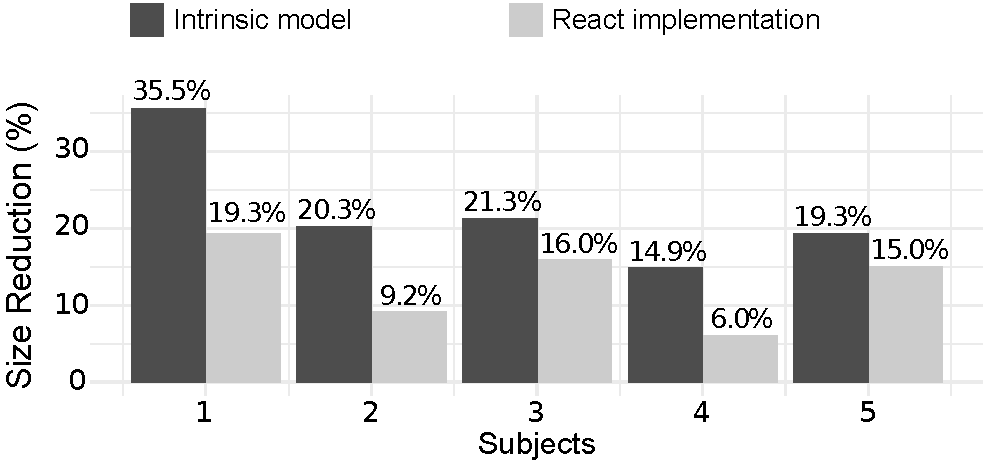
\includegraphics[width=0.75\textwidth]{maintainability/figures/size-reduction}
    \caption{Code reusability achieved by the proposed component generation, as measured by final size reduction.}
    
    \label{fig:size-reduction-results}
\end{figure} 

\begin{comment}

\begin{table}
	\caption{Size Reduction in the Mockup's \html}
	\centering
	%\fontsize{7pt}{8pt}\selectfont
	\setlength\tabcolsep{3px}
	\begin{threeparttable}
		%\bgroup
		%\def\arraystretch{1.4}
		\begin{tabular}{c c c c r r}
			\toprule
			\multirow{2}{*}{\textbf{Subject}}
				& \multicolumn{2}{c}{\textbf{\#Identified Refactoring Opportunities}} 
								&	& \multicolumn{2}{c}{\textbf{\%Size Reduction}}  \\ 
				\hhline{~--~--}
				& \textbf{\#Components}
						& \textbf{\#Component Instances}
								& 	& \textbf{Algorithm}
											& \textbf{\react} \\  \toprule
			1	&  5	& 29	&	& 35.54	& 19.34 \\
			2	&  5	& 17	&	& 20.27	&  9.20 \\
			3	&  5	& 26	&	& 21.33	& 16.00 \\
			4	&  6	& 21	&	& 14.90	&  6.01 \\
			5	&  4	& 17	&	& 19.34	& 15.01 \\ \midrule
\textbf{Avg.}	&  \textbf{5}	
						& \textbf{22}	
								&	& \textbf{18.96}
										 	& \textbf{11.56}  \\ \bottomrule
		\end{tabular}
		%\egroup
	\end{threeparttable}
	\label{table:size-reduction-results}
\end{table}

\end{comment}


\Cref{fig:size-reduction-results} illustrates the results of applying the proposed refactorings
on the test subjects.
Observe that, using \react implementation,
refactoring UI components results in reducing the size of the \html code
by 6\%--19.34\%, with an average of 11.56\%.
The \textit{intrinsic} performance of the algorithm itself, however, is higher: 14.90\%--35.54\%,
with an average of 18.96\%.
This difference highlights that \react components require quite considerable amount of added code
to the original \dom information of the UI component instances.
For example, a UI component shown in \Cref{fig:intermediate-model-sample-dom-subtrees}(d)
needs to be wrapped into a function named \code{render} implemented in a
\javascript class that extends the internal \react class, \code{React.Component}.
We also need to add additional code to pass arguments to the UI components for each UI component instance.
As mentioned, using another UI framework can yield different saving ratios. It is for these reasons that reporting the intrinsic performance is important.

It is worth mentioning that this saving is not meant to replace existing techniques
that, for instance, minify \html by removing white space, or via any other reduction approach.
Rather, whatever savings obtained from the components can complement them by adding even more saved bytes on top of what they would normally save.


\section{Discussion}
\header{Context within web development} The approach we present in this chapter refactors repetitions in the UI and merges them into a template, which is finally converted into a component in one of the common front-end frameworks (e.g., \react, \angular). This automates one of the initial steps in making a full-fledged web app UI, which is often time consuming and is done manually. The use of this approach, of course, would not mean that the web app is ready to launch to clients and the development process is finished. The developer would use these components and continue the development, by, e.g., adding business logic, handling events, connecting to databases or other sources. Furthermore, the approach we present in this chapter is for modularizing the UI view itself, and is therefore orthogonal to the remaining components of the architecture pattern of the app (e.g., Model-view-controller (MVC), Model-view-presenter (MVP)) and to any backend server functionality.

\header{Threats to validity}
We chose test subjects (i.e., mockups) randomly from the Internet
with the mentioned criteria in \Cref{sec:study-design},
to avoid any selection bias.
Plus, the evaluation participants are expert web developers
with different years of web development experience,
mitigating the threats to the internal validity of the study.
The mockups are diverse and complex enough
to be representative of real-world app front-ends,
mitigating the external validity of the study by making the results generalizable.
To make the study replicable, we have made 
\toolname's source code, evaluation subjects, and the anonymized participants' responses available online~\cite{tool-and-data}.
% !TEX root =  paper.tex

\section{Related Work}
\label{section:related-work}

\header{Visual analysis}
There exist a few techniques that analyze web applications from a visual perspective.
Choudhary et al.~\cite{choudhary2012crosscheck} propose an approach that detects cross-browser compatibility by examining visual differences between the same app running in multiple browsers.
Burg et al.~\cite{burg2015explaining} present a tool that helps developers understand the behavior of front-end apps. It allows developers to specify which element they are  interested in, then tracks that element for any visual changes and the corresponding code changes.
Bajammal et al.~\cite{canvas_icst2018} propose an approach to analyze and test web canvas element through visual inference of the state of the canvas and its objects, and allowing canvas elements to be testable using common DOM testing approaches.
In contrast to our work, none of these studies aims to automatically identify and extract web components. Stocco et al.~\cite{2018-Stocco-FSE, 2018-Leotta-STVR} explore visual techniques for web testing applications, including visual-based test repair and techniques for migrating DOM-based tests to visual tests.

\header{Clone detection}
There is a large body of work on clone detection 
in conventional source code~\cite{Roy:2007:CloneSurvey, Roy:2009:ComparisonOfCloneDetectionTechniques, Rattan:2013:CloneDetectionSystematicReview}. Some techniques also exist targeting web artifacts, such as for identifying duplicated content~\cite{Boldyreff:2002:ReverseEngineeringMaintainableWWW} or
script function clones~\cite{Lanubile:2003:FindingFunctionClones, Calefato:2004:FunctionCloneDetection},
and quantifying the structural similarity across pages~\cite{DeLucia:2005:UnderstandingClonedPatterns}.
A number of existing publications~\cite{template_1, template_2, template_3, template_4} propose template identification for Java code by defining a number of heuristics to compute code similarity.
Rajapakse and Jarzabek~\cite{Rajapakse:2005:AnInvestigationOfCloning} use CCFinder~\cite{Kamiya:2002:CCFinder}
to identify duplication in web applications.
Synytskyy et al.~\cite{Synytskyy:2003:ResolutionOfStatic} use an \textit{island grammer} 
to identify cloned \html forms and tables.
Cordy et al.~\cite{Cordy:2004:PracticalLanguageIndependent} propose a language-independent technique
to identify exact/near-miss clones (initially in \html) using island grammars, pretty-printing and textual differencing. 
Inspired by that work, \nicad clone detector is proposed~\cite{Roy:2008:NiCad}.

\header{Transformation and refactoring}
Various techniques are proposed to convert static pages to dynamic ones~\cite{Boldyreff:2002:ReverseEngineeringMaintainableWWW, Synytskyy:2003:ResolutionOfStatic}, to 
generalize dynamic web pages~\cite{Lucia:2004:ReengineeringWeb, Rajapakse:2007:Unifying},
or to find similar functionalities across web pages~\cite{DeLucia:2005:UnderstandingClonedPatterns}. Other techniques~\cite{mesbah:migrate07} use clustering to group similar static web pages together to extract single-page templates. 
Pattern mining techniques are used~\cite{Mazinanian:2014:RefactoringCSS, Davood:2016:ASE:CSSMigration, Davood:ICSE:2017:CSSDev} for identifying and refactoring duplicated \css code in web apps.
In contrast to our work, none of these studies aims at automatically identifying and extracting web components from mockups.
% !TEX root =  paper.tex

\section{Conclusions}
\label{section:conclusions}
The development of a web app front-end involves multiple stakeholders, chief among them the graphics designer and web developer. A UI mockup designed by the graphics designer has to be analyzed and processed by a web developer in order create the app's front-end code, a task that is laborious and involves manual time consuming steps. In this chapter, we proposed an approach to automate this aspect of web development by generating reusable web components from a mockup. We conducted an evaluation on real-world web mockups and assessed the quality of generated components through comparison with expert developers. An average of \precision precision and \recall recall was achieved in terms of agreement with the developers' assessment, the refactorings were performed in a correct manner, and the components achieved a 22\% reusability, on average.
	
%\bibliography{bibliography}
% !TEX root =  manuscript.tex
\section{Conclusions}\label{sec:conclusions}
A recent and growing trend in software engineering 
research is to adopt a \emph{visual perspective} of 
the software, which entails extracting and processing 
\textit{visual artifacts} relevant to the software being analyzed. 
To gain a better understanding of this trend,
in this chapter, we surveyed the literature on the use of 
visual analysis approaches in software engineering. 
From more than \initialPoolSize publications, 
we systematically obtained \numberOfPapers papers 
and analyzed them according to a number of research dimensions.
Our study revealed that visual analysis techniques 
have been utilized in all areas of software engineering, 
albeit more prevalently in the software testing field.
We also discussed why visual analysis was utilized, 
how these techniques are evaluated, and what limitations they bear.
Our suggestions for future work include the development 
of common frameworks and visual benchmarks to collect 
and evaluate the state-of-the-art techniques, 
to avoid relying on ad-hoc solutions. We believe that 
the findings of this work illustrate the potential of 
visual approaches in software engineering, and may help 
newcomers to the field in better understanding the research landscape.

\hl{A number of key findings can be observed from the survey in order to help in 
guiding and framing the remainder of the dissertation. 
First, cross-browser testing is by far the most common area of application, 
whereas exploring non-functional properties received little to no focus. 
This shows that there is an opportunity to explore the use of visual analysis 
in improving non-functional properties, and therefore the remainder of the dissertation 
will be focusing on this aspect. This will provide better and more novel research 
contributions compared to exploring functional properties. 
Furthermore, our survey of the visual analysis techniques used shows that the 
majority of existing works use some form of basic image diffing or features. This shows that it would be novel and potentially useful to investigate more fine-grained level of visual analysis that examines fine-grained visual details. Accordingly, this unexplored approach will be the basis of the techniques proposed in the remainder of the dissertation.}  


\balance




% Generally recommended to put each chapter into a separate file
%\include{relatedwork}
%\include{model}
%\include{impl}
%% !TEX root =  manuscript.tex
\section{Discussion}\label{sec:discussion}

\header{Increasing Adoption of Visual Approaches}
Our findings show a general growth trend in the adoption and use of visual approaches
in the SE community.
Most of the surveyed papers explicitly recognize, and empirically
demonstrate, the contribution brought by visual methods in supporting SE tasks.

Based on our examination of the literature,
we attribute this increase to two factors.
First, many software developed nowadays have a GUI or other visual interfaces.
The end-user experience is increasingly becoming more important in adding value
to software, and therefore the adoption of visual methods is expected to
increase further in the next years.
Our examination of the trend of number of annual publications 
already shows this trend of increasing number of works utilizing 
visual techniques.
Second, the rapid pace of improvement in hardware and processor architecture has made
the efficiency and run time of advanced visual techniques feasible in common
development environments, which we expect will cause an increased adoption of
visual approaches further down the line.

\header{Software Testing a Major Driver of Visual Approaches}
The majority of papers (around 75\%) have focused on the research area of
software testing.
Our intuition behind this is two-fold.
First, testing is one of the most active SE research areas in general,
so it is not surprising that most of the collected papers fall
within this category.
Second, testing is largely a tooling-based research area, in which
tool prototypes are developed and empirically evaluated.
Many different static and dynamic analysis tools are proposed each year
to facilitate test engineers' activities. 
The results of this survey show that the visual perspective of the software
has been recently used to complement static and dynamic analysis because
it provides a novel and complimentary perspective of the software under test.
The types of analyses that are performed on the presentation-level of the
application would be likely very difficult to perform by analyzing the source code only,
especially with the increasingly complex interfaces and the great emphasis
placed on user experience, of which the interface is a cornerstone component.


\header{Custom Solutions}
The visual techniques used in the collected papers are often ad-hoc solutions developed for tackling a specific problem. 
Authors recognize that it is unlikely to have a consolidated and broadly-accepted solution.  
More specifically, all collected papers have discussed, to some extent, the need of visual approaches for parameter fine-tuning, such as optimal threshold selections. 
In contrast, as will be discussed in the next chapters, the 
techniques proposed in this dissertation aim to minimize or eliminate the need for parameters or thresholds whenever possible. 

Manipulating visual artifacts through a visual technique is highly application-specific, both in the adopted approach and in the considered domain~\cite{2020-Yandrapally-ICSE}. 
For instance, this survey highlights a large body of work in the area of
cross-browser incompatibility.
The authors of these papers have adopted a large variety of solutions
(or incremental variations) to tackle the same problem.
To mention a few,~\citet{Choudhary-2010-ICSM} use an image comparison measure
based on Earth Mover's Distance (EMD), whereas ~\citet{Mahajan-2015-ICST} adopt
perceptual differencing, and~\citet{He-2016-ICWS} compare the colour histograms,
among other approaches.
This trend can be partially explained by the need of proposing and experimenting
with novel and potentially useful techniques.
However, a researcher approaching this topic for the first time could be
somewhat disoriented.
In fact, given that the solutions for the same problem are many,
and they are often evaluated on different benchmarks,
it is not straightforward to find an agreement on what the best technique could be. 
This led to a landscape where each work would typically experiment with a custom
visual processing pipeline to address the specifics of the SE task at hand.

\header{Need for Visual Benchmarks in SE}
We highlight the lack of comparative visual benchmarks on which to evaluate
the plethora of visual approaches utilized in software engineering research. 
A repository of standard, well-organized, categorized, and labeled visual artifacts could
be very useful to support empirical experiments, and to guide
the next generation of research utilizing visual approaches
for software engineering tasks.
Such repositories exist in traditional
(non-visual) software engineering research,
such as SIR~\cite{Do:2005:SCE:1089922.1089928},
Defects4J~\cite{Just:2014:DDE:2610384.2628055}, SF100~\cite{sf100}, and BugsJS~\cite{bugsjs:icst19,2020-Gyimesi-STVR}. This has not been the case, however, for visual techniques in software engineering.
For instance, having analogous repositories for visual bugs can foster
further applications of visual methods in software testing. 
In the issues discussed in this dissertation, which are all non-functional properties, no visual benchmarks exist either, since 
the field is still at its early stages and hasn't matured yet to the degree of creating benchmarks. 

Similarly, object detection and classification tasks need labeled images.
In computer vision literature, there exist some pre-validated and labeled visual
benchmarks, such as ImageNet~\cite{Russakovsky:2015:ILS:2846547.2846559},
BSDS500~\cite{MartinFTM01}, or Caltech 101~\cite{Fei-Fei:2006:OLO:1115692.1115783}.
In software engineering,
a benchmark of labeled visual artifacts might
aid in developing visual techniques,
or training systems for machine learning and deep learning
scenarios.
A notable step in this direction has been carried out 
in the Rico~\cite{Deka-2017-UIST} repository. 
The repository contains around 70k labeled UI screenshots, 
each of which are labeled with 
visual, textual, structural, and interaction trace data.
The dataset facilitates software engineering tasks 
related to the UI, such as UI design search, UI layout generation, 
and UI code generation.


\header{Maintainability of Visual Artifacts}
The visual artifacts created or extracted from the software 
are rarely static across time,
especially for rapidly evolving software such as in agile environments.
The artifacts would therefore have to be frequently modified
or updated to keep track of the underlying evolving software.
\citet{Alegroth-2013-ICST} indicate that
the maintainability of visual artifacts
produced and used by the visual testing tools
as being a major challenge of the
visual-based testing approaches.
Potential research directions to mitigate this challenge 
include proposing strategies for conducting cost-benefit analysis
depending on the expected degree of visual evolution of the software,
and devising automated techniques to
help with or reduce the maintainability
effort for visual artifacts. 


\header{Familiarity with Computer Vision}
Perhaps the biggest challenge hindering a wider adoption
of visual approaches in software engineering
is the lack of familiarity with computer vision techniques.
For instance,
\citet{Delamaro-2011-STVR} describe how developers
should have basic knowledge of image processing
in order to even \textit{use} the proposed tool in the paper.
This is because the visual artifacts can structurally vary with each use,
and thus sometimes one or more manual image processing adjustments
need to be performed before being able to process the visual artifacts. 
In the work proposed in this dissertation, we mitigate this issue 
by proposing techniques that reduce or eliminate the need for parameters or adjustment thresholds, in order to improve robustness. 

\header{Threats to Validity}
The threats to validity of this survey are the bias in the papers' selection and misclassification of the pool of papers in the various research questions. We mitigate these threats as follows.
Our paper selection was driven by the keywords related to visual approaches and software engineering (see Section~\ref{sec:collection}). 
We may have missed studies that use visual methods in the software engineering activities that are not captured by our terms list.
To mitigate this threat, we performed an issue-by-issue manual search of the major software engineering conferences and journals, and followed through with a snowballing process.
Concerning the papers' classification, we manually classified all selected papers into different categories based on the targeted SE area, as well as, more fine-grained sub-categories based on their domains, tasks, and the utilized visual methods (see Section~\ref{sec:results}). 
\changed{Identifying the rationale from the papers that do not explicitly mentioned it  involved some subjectivity and may have resulted in suboptimal mappings, which constitutes another threat.} However, there is no ground-truth labeling for such classification. To minimize classification errors, the first three authors of this chapter have carefully analyzed the full text and performed the classifications individually. Any disagreements were resolved by further discussion.

%% !TEX root =  manuscript.tex
\section{Conclusions}\label{sec:conclusions}
A recent and growing trend in software engineering 
research is to adopt a \emph{visual perspective} of 
the software, which entails extracting and processing 
\textit{visual artifacts} relevant to the software being analyzed. 
To gain a better understanding of this trend,
in this chapter, we surveyed the literature on the use of 
visual analysis approaches in software engineering. 
From more than \initialPoolSize publications, 
we systematically obtained \numberOfPapers papers 
and analyzed them according to a number of research dimensions.
Our study revealed that visual analysis techniques 
have been utilized in all areas of software engineering, 
albeit more prevalently in the software testing field.
We also discussed why visual analysis was utilized, 
how these techniques are evaluated, and what limitations they bear.
Our suggestions for future work include the development 
of common frameworks and visual benchmarks to collect 
and evaluate the state-of-the-art techniques, 
to avoid relying on ad-hoc solutions. We believe that 
the findings of this work illustrate the potential of 
visual approaches in software engineering, and may help 
newcomers to the field in better understanding the research landscape.

\hl{A number of key findings can be observed from the survey in order to help in 
guiding and framing the remainder of the dissertation. 
First, cross-browser testing is by far the most common area of application, 
whereas exploring non-functional properties received little to no focus. 
This shows that there is an opportunity to explore the use of visual analysis 
in improving non-functional properties, and therefore the remainder of the dissertation 
will be focusing on this aspect. This will provide better and more novel research 
contributions compared to exploring functional properties. 
Furthermore, our survey of the visual analysis techniques used shows that the 
majority of existing works use some form of basic image diffing or features. This shows that it would be novel and potentially useful to investigate more fine-grained level of visual analysis that examines fine-grained visual details. Accordingly, this unexplored approach will be the basis of the techniques proposed in the remainder of the dissertation.}  


\balance


%    3. Notes
%    4. Footnotes

%    5. Bibliography
\begin{singlespace}
\raggedright
\bibliographystyle{abbrvnat}
\bibliography{biblio}
\end{singlespace}

%\appendix
%    6. Appendices (including copies of all required UBC Research
%       Ethics Board's Certificates of Approval)
%\include{reb-coa}	% pdfpages is useful here
%%\chapter{Supporting Materials}
%
%This would be any supporting material not central to the dissertation.
%For example:
%\begin{itemize}
%\item additional details of methodology and/or data;
%\item diagrams of specialized equipment developed.;
%\item copies of questionnaires and survey instruments.
%\end{itemize}


\backmatter
%    7. Index
% See the makeindex package: the following page provides a quick overview
% <http://www.image.ufl.edu/help/latex/latex_indexes.shtml>


\end{document}
